\documentclass[12pt,a4paper]{basque-book}
\usepackage[utf8]{inputenc}


\usepackage{times}
\usepackage[basque]{babel}
\renewcommand{\=}{"-}
\selectlanguage{basque}
\input formatoa
%\usepackage[latin1]{inpuntenc}
\usepackage[T1]{fontenc}
\usepackage{graphicx}
% Mikel : Nik gehitutako paketeak
%\usepackage[english]{babel}
\graphicspath{ {0-title/figures/}
               {2-Sarrera/figures/}
               {3-MetodoSinplektikoak/figures/} 
               {4-Problemak/figures/}
               {5-KomaHigikorra/figures/} 
               {6-ZientziaKonputazioa/figures/} 
               {7-IRKPuntuFinkoa/figures/}
               {9-IRKNewton/figures/}
               {10-IRKEguzkiSistema/figures/}
               {21-Eztabaida/figures/}
               {22-Konlusioak/figures/}
               {B-Eranskina/figures/}}
\usepackage{listings}   % kodea azaltzeko
%\usepackage[ruled]{algorithm2e}
%\usepackage[linesnumbered,ruled,vlined]{algorithm2e}
\usepackage{algorithm2e}
\SetAlFnt{\footnotesize}
\SetAlCapFnt{\small}
\SetAlCapNameFnt{\small}


\renewcommand{\algorithmcfname}{Algoritmoa}
\usepackage {amsmath,amsfonts,amssymb}
\usepackage{subfig}
\usepackage{tikz}
\usepackage{epigraph}
\usepackage{csquotes}

%Higham (bibliostyle)
\usepackage{texnames}
\usepackage{url}
\usepackage{color}
\usepackage{graphicx}
\definecolor{hotpink}{rgb}{0.9,0,0.5}
\usepackage[colorlinks,urlcolor=blue,citecolor=hotpink,linkcolor=blue]{hyperref}
\def\ycite[#1#2#3#4#5]#6{\cite[$\mit{#1#2#3#4}$#5]{#6}}

\usepackage{makeidx}
\makeindex

% End-Mikel

% ShareLatex (listings)
\definecolor{codegreen}{rgb}{0,0.6,0}
\definecolor{codegray}{rgb}{0.5,0.5,0.5}
\definecolor{codepurple}{rgb}{0.58,0,0.82}
\definecolor{backcolour}{rgb}{0.95,0.95,0.92}
 
\lstdefinestyle{mystyle}{
    backgroundcolor=\color{backcolour},   
    commentstyle=\color{codegreen},
    keywordstyle=\color{magenta},
    numberstyle=\tiny\color{codegray},
    stringstyle=\color{codepurple},
    basicstyle=\footnotesize,
    breakatwhitespace=false,         
    breaklines=true,                 
    captionpos=b,                    
    keepspaces=true,                 
%    numbers=left,                    
    numbersep=5pt,                  
    showspaces=false,                
    showstringspaces=false,
    showtabs=false,                  
    tabsize=2
}
\lstset{style=mystyle}
% End ShareLatex (listings)

\pagenumbering{roman} %Required by SGPS

\newcommand{\M}{\mathcal{M}}
\newcommand{\N}{\mathcal{N}}
\renewcommand{\P}{\mathcal{P}}
\newcommand{\Q}{\mathcal{Q}}
\newcommand{\F}{\mathbb{F}}
\newcommand{\fl}{\mathrm{fl}}
\newcommand{\R}{\mathbb{R}}
\renewcommand{\algorithmcfname}{Algoritmoa}
\renewcommand{\leq}{\leqslant}
\renewcommand{\geq}{\geqslant}
\renewcommand{\dim}{d}
\newcommand{\eps}{\varepsilon}
\newcommand{\half}{\textstyle \frac12}

\begin{document}


%: ----------------------- generate cover page ------------------------

\frontmatter
%Title page
%%%%%%%%%%%%%%%%%%%%%%%%%%%%%%%%%%%%%   frontpage  %%%%%%%%%%%%%%%%%%%%%%%%%%%%%%%%%%%%%%%%%%%%%%%5
\begin{titlepage}
\newcommand{\HRule}{\rule{\linewidth}{0.5mm}}
\begin{center}
%\includegraphics[width=0.3\textwidth]{uwo.eps}\\[1cm]    
\HRule \\[0.4cm]
%{ \Large \bfseries \sc N-Gorputzeko problema grabitazionalaren ebazpenerako zenbakizko metodoen azterketa.}\\[0.4cm]
{ \Large \bfseries \sc Runge-Kutta metodo inplizitu sinplektikoen inplementazio eraginkorra, eguzki-sistemaren simulaziorako aplikazioarekin.}\\[0.4cm]
% maximum of 60 characters for spine title
%{(Spine title: Backward Error Analysis as a Model of Computation)\\ (Thesis Format: Integrated-Article)}



\HRule \\[1cm]
%by
%\\[1cm]
{\Large Mikel Antonana Otano}
\\[.75cm]


%{\large Graduate Program in Applied Mathematics}
%\\[1.2cm]
%{\large A thesis submitted\\ in partial fulfillment of the requirements for\\ the degree of Master of Science}
%\\[.5cm]
{\large Konputazio zientzia eta Adimen Artifiziala saila \\[.1cm]
}
{\large Informatika fakultatea \\[2.cm]
}



\includegraphics[scale=1.5]{Ehu-Logoa}
\\[5cm]

{\large Doktorego tesia\\[.1cm]}
{\large Donostia 2017}




%\copyright Mikel Antonana 2017
\end{center}
\end{titlepage}\pagebreak %title page in a subfile. Optional, but looks nicer.
%\addtocounter{page}{1}

%\title{N-Gorputzeko problema grabitazionalaren ebazpenerako zenbakizko metodoen azterketa.}

%\author{ Mikel Antoñana Otaño}
%\date{Otsaila 2014}

%\begin{titlepage}
%\maketitle
%\end{titlepage}


%: ----------------------- contents ------------------------

\setcounter{secnumdepth}{3} % organisational level that receives a numbers
\setcounter{tocdepth}{0}    % print table of contents for level 3
%\tableofcontents

{\expandafter\def\csname @starttoc\endcsname#1{\InputIfFileExists{\jobname.#1}{}{}}%
\tableofcontents}


\renewcommand*\contentsname{Gaien Aurkibidea (detailed)}

\setcounter{tocdepth}{3}    % print table of contents for level 3
\tableofcontents



%: ----------------------- list of figures/tables ------------------------

%\newpage
%\listoffigures
%\newpage
%\listoftables
%\newpage



%\begin{abstract}  
 
%\keywords{First keyword \and Second keyword \and More}
% \PACS{PACS code1 \and PACS code2 \and more}
% \subclass{MSC code1 \and MSC code2 \and more}
%\end{abstract}


%: --------------------------------------------------------------
%:                  MAIN DOCUMENT SECTION
% --------------------------------------------------------------

\mainmatter

\chapter*{}
\epigraph{Itxaropena ez da dena ondo aterako den konbentzimendua; nolanahi ateratzen dela ere, egiten dugunak zentzua duen ziurtasuna baizik.}
{\textit {Vaclav Havel}}


\part{Introduction}
\chapter{Sarrera.}


\section{Ikerketaren testuingurua.}

Urte luzez, zientziaren arlo ezberdinek N-gorputzeko problema ikertu dute. Astronomoek eguzki-sistemaren planeten mugimendua ulertu nahian egindako lanak edo kimikariek erreakzio kimikoekin esperimentatzeko molekulen dinamikaren azterketak aipatu daitezke. Gainera,  N-gorputzen problemaren azterketak garrantzi berezia izan du matematikako eremu ezberdinen garapenean,  dinamika ez-lineal eta kaos teorian esaterako. 

Garai batean, N-gorputzen problemak teori analitikoen bidez aztertzen ziren baina konputagailuen sorrerarekin, zenbakizko integrazioak tresna nagusia bilakatu ziren. Azken hamarkadetan, bai konputazio teknologien aurrerapenari esker bai algoritmo berrien sorrerari esker, zenbakizko azterketek garapen handia izan dute. Zenbakizko simulazioen laguntzaz, eguzki-sistemaren dinamikaren funtsezko galdera batzuk ezagutu ditugu eta berriki, Karplusen taldeak 2013. urteko kimika Nobel saria \cite{Karplus2014} jaso du kimika konputazionalean egindako lanarengatik.       

Guk lan honetan, N-gorputzen problema grabitazionala aztertuko dugu. Oro har eta gaia kokatzeko asmoarekin, N-gorputzen ohiko zenbakizko  integrazioak hiru taldetan sailkatu ditzakegu:
\begin{enumerate}
{
\item Epe motzeko eta doitasun handiko integrazioak. 
 Eguzki-sistemaren efemeride zehatzak \cite{Folkner2014} edo espazioko satelite artifizialen kokapenen \cite{Beylkin2014} kalkuluetarako erabili ohi dira.
\item Epe luzeko baina doitasun txikiko integrazioak.
 Denbora epe luzean, planeta-sistemen mugimendua ezagutzeko egindako ikerketak dira. Azterketa hauetan, helburua gorputzen mugimenduaren argazkia orokorra (zehaztasun handirik gabe) ezagutzea da. Normalean, problema mota hauetan gorputzen arteko kolisio gertuko egoerak ez dira izaten.     
\item N-gorputz kopurua edozein izanik , hauen arteko kolisioak gerta daitezkeen problemak.
 Integrazio hauetan, konplexutasun handiari aurre egin behar zaio. N-gorputz kopurua miliotakoa \cite{Ishiyama2012} izan dateke eta kolisio gertuko egoeren ondorioz, kalkuluetan egindako zenbakizko errore txikiek soluzioan eragin handia izan ditzakete.    
}
\end{enumerate}

Gure helburua, eguzki-sistemaren epe luzeko eta doitasun handiko integrazioetarako inplementazio eraginkorra garatzea da. Aurreko hamarkadetan, eguzki-sistemaren planeten epe luzeko zenbakizko integrazioa erronka garrantzitsua izan da. Adibidez, Sussmanek eta Wisdomek \ycite[1993]{Sussman1992} eguzki sistemaren 100 milioiko integrazioarekin, planeten mugimendua kaotikoa zela baieztatu zuten. Aldi berean, paleoklimatologi-zientzialariak orain milioika urte gertatutako klima zikloak (epel, hotz eta glaziazio aroak) azaltzeko, lurraren orbitan izandako aldaketaren eraginez gertatu zirela azaltzen duen teoria (Milankovitch 1941) \cite{Berger2012} baieztatzeko, planeten orbiten efemeride zehatzetan oinarritu dira.        

Epe luzeko integrazio hauetarako zenbakizko hainbat metodo erabiltzen dira, bereziki beren izaera Hamiltondarra mantentzen duten metodoak (metodo sinplektikoak).

Konputazio-teknologi aurrerapenak handiak izan arren, eguzki-sistemaren simulazio hauek konputazionalki oso garestiak dira eta exekuzio denbora luzeak behar dituzte; adibidez, Laskarrek \ycite[2010]{Laskar2011} bere azken integrazioa burutzeko 18 hilabete behar izan zituen.
Azken urteotako konputagailu berrien arkitekturaren bilakaerak, algoritmo azkarren diseinua aldatu du: simulazioak azkartzeko algoritmoak paralelizazioan oinarritu behar dira. Azpimarratzekoa da ere, integrazio luze hauen erronka handienetako bat, biribiltze errorearen garapena zaintzea da, non errorearen edozein joera ekiditen den \cite{Laskar2015}.
 

\section{Motibazioa.}
\label{intro}


Metodo sinplektikoen artean erabilienak, izaera esplizituko algoritmoak dira. Oro har problema zurruna ez bada, metodo esplizituak  metodo inplizituak baino eraginkorragoak dira. Metodo inplizituetan ekuazio sistema ez-lineala askatu behar da (eragiketa garestia) eta honek, metodo esplizituekiko CPU denbora gainkarga suposatzen du. Horregatik problema zurruna ez denean, metodo esplizituak erabili ohi dira eta problema zurruna denean bakarrik jotzen dugu metodo inplizituengana. Epe luzeko eguzki-sistemaren integrazioetarako, baieztapen hau eztabaidagarria dela, eta praktikan metodo inplizituetan gehiago sakondu behar dela iruditzen zaigu. 

Lan honetan, Gauss zenbakizko integrazio metodo sinplektikoaren azterketa egingo dugu. Hainbat autorek (Hairer \cite{Hairer2006}\cite{Hairer2008} eta Sanz Serna\cite{JMSanz-Serna1994}) metodo honen potentziala nabarmendu dute. Azken urtetan, espazioko satelite artifizialen arloan ere, Gauss integrazio metodo inplizituarekiko interesa azaldu dute \cite{Bradley2014}\cite{Beylkin2014}. 

Jarraian, Gauss metodo inplizituen ezaugarri interesgarri batzuk nabarmenduko ditugu. Abantaila nagusienetakoa malgutasuna da.  Metodo inplizituek inplementazio malgua onartzen dute eta ondorioz, integratu nahi dugun problemari egokitzeko eta eraginkortasuna hobetzeko aukera ezberdinak eskaintzen dizkigu. Aipatzekoa da ere, metodo esplizituak (sinplektikoak) sistema Hamiltondar banagarrietan bakarrik aplika daitezkeela eta orduan, Hamiltondarraren egitura hau aprobetxatuz oso eraginkorrak direla. Baina metodo inplizituak aldiz, Hamiltondar orokorrei aplika daitezke eta gainera, lehen ordenako ekuazio diferentzialetarako  metodo sinplektikoak, inplizituak izan behar dira. Gainera, Gauss metodoak paralelizagarriak dira, hau da, ekuazio diferentzial konplexuak kalkulatu behar ditugunean, $s$-ataletako funtzio konputazioak paraleloan exekutatu daitezke. Azkenik ez dugu ahaztu behar, orden altuko Gauss metodoak existitzen direla  eta hauek beharrezkoak ditugula doitasun handiko integrazioetarako.     

\paragraph*{}Atal hau bukatzeko, Sanz Sernaren  \ycite[1992]{Sanz-Serna1992} hitzak berreskuratuko ditugu. 
\begin{displayquote}
On the other hand, little has been undertaken in the construccion of practical high-order methods and the design of serious symplectic software is still waiting consideration.
\end{displayquote}

\section{Helburua eta esparrua.}

Gure helburua, eguzki-sistemaren epe luzeko integraziorako Gauss metodo inplizituaren inplementazio eraginkorra proposatzea da. Helburu hau lortzeko, honako aspektu hauek bereziki zainduko ditugu: eguzki-sistemaren problemaren ezaugarriak, biribiltze errorearen garapena eta egungo konputagailuen gaitasunari egokitutako algoritmo azkarren diseinua.  

N-gorputzeko problema grabitazionalari dagokionez, eguzki-sistemaren eredu sinplea integratuko dugu. Eguzki-sistemaren gorputzak masa puntualak kontsideratuko ditugu eta gure ekuazio diferentzialek, gorputz hauen arteko erakarpen grabitazionalak bakarrik kontutan hartuko dituzte. Beraz, eguzki-sistemaren eredu konplexuagoetako erlatibitate efektua, gorputzen formaren eragina, eta beste zenbait indar ez-grabitazionalak ez dira kontutan hartu.
Bestalde era honetako integrazioetan, gorputzen hasierako balio eta parametro zehatzak sateliteen bidez jasotako datu errealekin bat datozela egiaztatze prozesua ez dugu landu \cite{Laskar2015}.

Zeintzuk dira eguzki-sistemaren problemaren ezaugarri bereziak? Batetik, bi gorputzen problemaren  soluzio zehatza ezaguna eta eguzki-sistemaren gorputzen mugimenduaren konputazioaren oinarria da. Bestetik,  badugu gorputz nagusi bat (eguzkia) eta honen inguruan mugimenduan dauden gorputzak: barne planetak, masa txikikoak eta eguzkitik gertu daudenak ; kanpo planetak, masa handikoak eta eguzkitik urrun daudenak. Kanpo planeta nagusi hauen eboluzioa, eguzki-sistema osoaren zati garrantzitsuena da eta barne planeten mugimendua kontutan hartzeak ala ez, kanpo planeten zenbakizko integrazioarengan oso eragin txikia du. Eguzki-sistemaren egitura honi abantaila gehien ateratzen dion planteamendua bilatuko dugu.
  
Konputagailuen koma-higikorreko aritmetika ondo ulertzea garrantzitsua da. Zenbaki errealen adierazpen finitua erabiltzen denez, bai zenbakiak memorian gordetzerakoan, bai hauen arteko kalkulu aritmetikoak egiterakoan, biribiltze errorea sortzen da. Integrazio luzeetan, biribiltze errorea propagatzen da eta une batetik aurrera, soluzioen zuzentasuna ezereztatzen da. Zentzu honetan, doitasuna hobetzeko biribitze errorea gutxitzen duten teknika bereziak aplikatzea ezinbestekoa izaten da. Integrazio luzeetan, maiz doitasun handian lan egiteko aukera aipatzen da, baina doitasun altuko aritmetikaren ($128$-bit) inplementazioa software bidezkoa denez, oso motela da eta ez da erabilgarria. Exekuzio denbora onargarriak lortzeko tarteko irtenbideak landu behar dira, hain zuzen ere, doitasun ezberdinak nahasten dituzten inplementazioak.       

Konputagailu teknologiaren garapenean, algoritmo azkarren diseinua baldintzatzen duten bi ezaugarri azpimarratu behar dira. Batetik, konputagailuak orokorrean paraleloak dira eta algoritmo azkarrak garatzeko, kodearen paralelizazio gaitasunari heldu behar zaio. Bestetik, konputazioaren alde garestiena, memoria eta prozesadorearen arteko datu mugimendua denez, prozesadorearen konputazio handiena komunikazio txikienarekin lortu behar da. 

Sarrera honetan paralelizazioari buruzko ohar batzuk ematea komeni da. Algoritmo baten kode unitateak paraleloan exekutatzeak badu gainkarga bat eta beraz,  algoritmoaren exekuzioa paralelizazioaz azkartzea lortzeko,  unitate bakoitzaren tamainak esanguratsua izan behar du. Gure eguzki-sistemaren eredua sinplea da eta logikoa da pentsatzea eredu konplexuagoetan, paralelizazioak abantaila handiagoa erakutsiko duela. Bestalde, $N$-gorputzen kopurua handia den problemetan, hauen arteko interakzio kopuru $\mathcal{O}(N^2)$ handia kalkulatu behar da eta indar hauen hurbilpena modu eraginkorrean kalkulatzeko metodo ezagunak daude: \textit {tree code}\cite{Barnes1986} eta \textit {fast multipole method}\cite{Carrier1988} izeneko metodoak. Baina gure probleman gorputz kopurua txikia denez, teknika hauek gure eremutik kanpo utzi ditugu. 


\section{Ekarpenak.}

Tesiaren lana hiru ataletan banatu dugu. Lehen urratsean, Gauss metodoaren puntu finkoaren iterazioaren inplementazioa aztertu dugu eta gure inplementazioen oinarriak finkatu ditugu. Bigarren fasean, Gauss metodoaren Newton iterazioaren inplementazio eraginkorra lortzeko ahalegin berezia egin dugu. Problema zurruna denean, puntu finkoaren iterazio ez da eraginkorra eta Newton iterazioa aplikatu behar da. Gainera problema ez-zurruna izanik ere, Newton iterazioak interesgarriak izan daitezke; bereziki doitasun altuko (doitasun
laukoitza) konputazioetan iterazio metodoaren konbergentzia ezaugarri onak direla eta.  Hirugarren fasean ...

Jarraian, atal bakoitzean egindako ekarpena nagusienak laburtuko ditugu:

\begin{enumerate}
\item IRK puntu finkoa.

Gauss metodoaren puntu finkoaren inplementazioaren azterketa sakon bat egin dugu eta horretarako, Hairer-en inplementazioa \cite{Hairer2008} hartu dugu gure lanaren abiapuntua. Kalitatezkoa inplementazio hau hobetzeko aukerak ikusi ditugu eta inplementazio sendoago bat proposatu dugu. Gure ekarpenak hauek izan dira:  

\begin{enumerate}
\item Metodoaren birformulazioa.

Gauss inplizitua aplikatzen dugunean, metodoa definitzen duten biribildutako koefiziente errealak ($\tilde{a}_{ij}, \tilde{b}_i \in \mathbb{F}$) erabiltzen dira. Formulazio estandarra erabiliz, koefiziente hauek ez dute metodoa sinplektikoa izateko baldintza zehazki betetzen eta beraz, izaera sinplektikoaren propietate onak galtzen dira. Metodoaren birformulazio baliokide bat proposatu dugu, non sinplektizidade baldintza zehazki beteko duten koefizienteak modu errazean finkatu daitezkeen.

\item Geratze irizpide berria.

Orokorrean, Hairer-en inplementazioaren puntu finkoaren iterazioaren geratze irizpide zuzena dela ikusi dugu baina kasu batzuetan goizegi geratzen dela baieztatu dugu. Arrazoiak bi direla ikusirik, bere geratze irizpidea bi zentzutan garatu/zorroztu dugu. Lehenik, Hairer-en inplementazioan, hobekuntza neurtzeko ataletako diferentziaren norma batean oinarritzen da. Normaren independentea den geratze irizpidea aplikatzea zuzenagoa da, eta horregatik, ataletako edozein osagaiaren diferentzia txikitzen den bitartean iterazioan jarraitzea finkatu dugu. Bigarrenik, iterazioen hobekuntza ez du zertan beherakorra izan behar, eta okertzen diren tarteko iterazioak gerta daitezke. Arazo hau gainditzeko, iterazioren batean osagai guztien diferentzia handitzea gertatzen denean, seguritateko bi iterazio gehigarri emango ditugu, iteraziotik irten aurretik.   

\item Atalen espresioaren aldaketa.

Integrazioan batura konpensatu estandarra aplikatzen dugunean, zenbakizko soluzioa $\tilde{y}_n, e_n \in \mathbb{F}^d$ lortzen dugu non $\tilde{y}_n+e_n \approx y(t_n)$ den. Hori dela eta, metodoaren atalen espresioan $\tilde{y}_n$ ordez, $\tilde{y}_n+e_n$ erabiltzea proposatu dugu. Aldaketa honekin, zenbakizko soluzioaren doitasuna zerbait hobetuko dela espero da.

\begin{equation*}
Y_{n,i}=y_n + \left(e_n+ \sum_{j=1}^{s}\mu_{ij} L_{n,j} \right).
\end{equation*}
  
\item Biribiltze errorearen estimazioa.

Zenbakizko soluzioaren $\tilde{y}_n+e_n \approx y(t_n), \ n=1,2,\dots$ biribiltze errorearen estimazioa, doitasun txikiagoko bigarren zenbakizko soluzioaren $\hat{y}_n+\hat{e}_n \approx y(t_n), \ n=1,2,\dots$  diferentzia gisa kalkulatuko dugu.
Erabiltzaileari zenbakizko soluzioaren estimazioa ezagutzeko, exekuzio bakarrean  eta \emph{CPU} gainkarga txikiarekin, bi integrazioak sekuentzialki kalkulatzeko aukera eskainiko zaio. 


\end{enumerate}


\item IRK Newton.

\begin{enumerate}
\item Ekarpen nagusia.

$S$-ataletako IRK metodoa,  Newton iterazioaren bidez $d$-dimentsioko ekuazio diferentzial  sistemari aplikatzeko, urrats bakoitzean $sd \times sd$ tamainako hainbat ekuazio sistema (iterazio bakoitzeko bat) askatu behar dira. Atal honetan, jatorrizko $sd$-dimentsioko ekuazio sistema, $(s+1)d$ dimentsioko ekuazio-sistema baliokide moduan berridatziko dugu. Ekuazio-sistema baliokidea,  $d \times d$ tamainako $[s/2]+1$ matrize errealen \emph{LU}-deskonposaketa bidez askatuko dugu. Tamaina txikiko matrizeen LU deskonposaketa azkarra denez, konputazionalki eraginkorra izatea espero dugu.   

\item Doitasun laukoitzeko inplementazioa.

Doitasun laukoitzeko exekuzioetan, funtzio balioztapena oso garestia da eta funtzio balioztapenen kopurua gutxitzea bilatuko dugu. Newton osoa aplikatzen dugunean pena mereziko du, Gaussen Newton iterazioko inplementazioaren ekuazio lineala askatzeko metodo iteratiboa aplikatzea. 

\item Newton mixtoa.


\end{enumerate}
  

\item IRK Eguzki-sistema.

Hirugarren urratsean, eguzki-sistemaren epe luzeko integrazioan arituko gara. Ekarpen handiena, atalen hasieraketa berri bat aplikatzea da alde Kepleriarraren fluxuan oinarrituz. IRK metodoak eskaintzen digun malgutasunari esker eta N gorputzetako problema grabitazionalaren ezaugarriez baliatuz inplementazio ezberdinak egingo ditugu. Inplementazio hauen eraginkortasuna, egungo integratzaile sinplektiko esplizituekin konparatuko ditugu.

\item Birparametrizazioa.

Azken urratsean, esperimentalki, eguzki-sistemaren integrazioan  denbora birparametrizazio teknikaren aplikazio sinple bat erakutsiko dugu. Integratzaile sinplektikoak luzera finkoko urratsa eduki behar du eta zentzu honetan, birparametrizazioa eraginkortasuna hobetzeko beste bide bat da.      

\end{enumerate}        


\section{Tesiaren egitura.}

Tesiaren lehenengo $(1-5)$ kapituluetan, zenbakizko integrazio sinplektikoak eta zientzia konputazionalaren oinarriak azaldu ditugu. Bigarren kapituluaren lehen zatian, \emph{Zenbakizko integratzaile sinplektikoen} inguruko oinarrizko kontzeptuak azaldu ditugu. Kapitulu honen bigarren zatian, Gauss metodo estandarra deskribatu eta bere propietate nagusienak eman ditugu. Kapitulu honen azken zatian, eguzki-sistemaren integraziorako metodo sinplektiko eta esplizitu nagusienak laburtu ditugu. Hirugarren kapituluan, lan honetan zenbakizko esperimentuetan erabili ditugun hasierako baliodun problemen zehaztasunak eman ditugu. Laugarren kapituluan koma-higikorreko aritmetika murgildu gara eta biribiltze errorearen inguruko gaiak argitu nahi izan ditugu. Bostgarren kapituluan, egungo konputazio zientziaren hardware eta software kontzeptu nagusienak ezagutarazi nahi izan ditugu.     

Tesiaren $(6-8)$ kapituluetan, gure inplementazio berriak garatu ditugu eta zenbakizko esperimentuen bidez, hauen eraginkortasuna erakutsi dugu. Lehenik, $6$.~kapituluan Gauss metodoaren puntu finkoaren iterazioaren inplementazio berria eman dugu. Ondoren, $7$.~kapituluan Gauss metodoaren Newton iterazioaren inplementazio eraginkorrak azaldu ditugu. $8$.~kapituluan, eguzki-sistemaren integraziorako inplementazio deskribapena egin dugu.  

Tesiaren $(9-10)$ kapituluetan, gure hipotesiaren eztabaida eta lanaren konklusioak idatzi ditugu.

Tesiaren bukaeran, hiru eranskinetan lanaren informazio osagarria bildu dugu. A-eranskinean, tesian zehar erabilitako hainbat frogen zehaztapenak eman dira. B-eranskinean, garatutako kodeak bildu eta erabiltzaileari erabilgarri izan daitekeen informazioa laburtu dugu. Azkenik C-eranskinean, erabilitako notazioaren inguruko argibideak eman ditugu.

      
      
\section{Laburpena}


%\part{Background}
\chapter{Zenbakizko integratzaile sinplektikoak.}

\section{Sarrera.}

Lan honen xede nagusia, N-gorputzeko sistema grabitazionalaren problemen zenbakizko simulaziorako algoritmoak garatzea da. Era horretako problemen artean, eguzki-sistemaren epe luzeko simulaziorako inplementazioak aztertuko ditugu \cite{Kholshevnikov2007,Brumberg2013} . Gaur egun, era horretako simulaziorako hainbat zenbakizko metodo erabiltzen dira, bereziki bere izaera Hamiltondarra mantentzen duten metodo sinplektikoak \cite{Eggl2010,Saha1992,Farres2013}. Metodo horien artean, gehien erabiltzen direnak izaera esplizituko algoritmoak diren arren, metodo inplizituak, modu egokian inplementatuz gero, hauek baino eraginkorragoak izan daitezke. Gauss zenbakizko integrazio metodo inplizituaren inplementazio eraginkorra aztertuko dugu.   

Atal honen lehen zatian, zenbakizko integrazio metodoen inguruko oinarrizko definizioak eta kontzeptuak azalduko ditugu. 
Jarraian, sistema Hamiltondarren eta metodo sinplektikoen sarrera emango dugu. Ondoren, zenbakizko integratzaile sinplektiko nagusienak aztertuko ditugu: alde batetik, Runge-Kutta metodo sinplektikoak (inplizituak) ; beste alde batetik, konposizio eta splitting metodo sinplektikoak (esplizituak). Azalpenak ulergarriak izateko, zenbakizko metodo sinpletan (Euler metodoak) eta adibideetan oinarritu gara. 

\section{Zenbakizko integrazio metodoak}

\subsection{Oinarrizko kontzeptuak.}

Ekuazio diferentzial arruntak, egoera aldaketak dituzten problemen azterketarako eredu matematikoak dira \cite{Hairer2015}. Zientziaren eta ingeniaritzaren arlo askotan azaltzen zaizkigu: planeten mugimenduen ereduetan (astronomia), erreakzio kimikoen formulazioetan, molekulen dinamiken simulazioetan, zirkuitu elektronikoen diseinuan, populazio-hazkunde eta interakzioetan (biologian), ekonomi azterketetan, \ldots  

Ekuazio diferentzial arrunta, $y(t)$ soluzio ezezagunaren eta bere $\dot{y}(t)$ deribatuaren arteko erlazioa da. $t$ aldagaiak, maiz denbora adierazten du eta $y(t) \in \mathbb{R}^{d}$ soluzio bektorea da. Deribatua, modu esplizituan denbora eta egoeraren arabera  adierazi daitekeenean, era honetako ekuazioak ditugu,
\begin{equation}
 \label{eq:201}
\dot{y}(t)=f(t,y(t)). 
\end{equation} 
$\dot{y}$ notazioa erabiliko dugu $dy/dt$ adierazteko.

Ekuazio diferentzial arruntetarako hasierako baliodun problemetan,  $y(t_0)=y_0 \in \mathbb{R}^d$ hasierako balio bat finkatzen da, eta $f(t,y)$ funtzioa, $f: \mathbb{R}^{d+1} \longrightarrow \mathbb{R}^d, \ \ t_0$ ingurunean diferentziagarria bada, orduan hasierako baliodun problemaren soluzioa existitzen da eta bakarra da \cite{Hairer2006},
\begin{equation}
 \label{eq:ivp}
\dot{y}(t)=f(t,y(t)), \ \ \ y(t_0)=y_0.
\end{equation} 

Goiko ekuazio-sistema bektoriala (\ref{eq:ivp}), ekuazio-sistema modu eskalarrean idatziko dugu orokorrean erabiliko dugun notazioa argitzeko:
\begin{align*}
&\dot{y}^1(t)=f^1(t,(y^1(t),y^2(t),\ldots,y^d(t))), \\
&\dot{y}^2(t)=f^2(t,(y^1(t),y^2(t),\ldots,y^d(t))), \\
&\ldots\ \ ,\\
&\dot{y}^d(t)=f^d(t,(y^1(t),y^2(t),\ldots,y^d(t))),  \\
& y(t_0)=(y_{0}^1,\ y_{0}^2,\ \ldots \ , \ y_{0}^d).
\end{align*}


Oso problema gutxitarako aurki daiteke ekuazio diferentzial arrunten soluzioa analitikoa (funtzio ezagunen araberako soluzio zehatza) eta beraz, ia problemak gehienak zenbakizko integrazio metodoen bidez ebazten dira.
Zenbakizko integrazioetan, soluzioaren hurbilpena,
\begin{align*}
 y_n \approx y(t_n), \ t_n=t_{n-1}+h_n, \ n=1,2,\dots
\end{align*}
une diskretu konkretuetarako, zehaztutako tarte batean ($t_0\le t \le t_f$) lortuko da. Zenbakizko soluzioa, sekuentzialki urratsez-urrats kalkulatzen da eta lortutako balio  multzoak $(t_0,y_0),(t_1,y_1),\dots,(t_f,y_f)$ zenbakizko soluzioa definitzen du.   

Zenbakizko soluzioaren ($y_n$) kalitatea, bi errore mota nagusien araberakoa izango da: zenbakizko integrazio metodoak sortutakoa (trunkatze errorea) eta konputazioan aritmetika finituak eragindakoa (biribiltze errorea). 

Ekuazio diferentziala beti \emph{sistema autonomo} moduan, hau da, denborarekiko independentea, idatz daiteke. Hori horrela izanik, notazioa sinplifikatzeko era honetako hasierako baliodun problemak kontsideratuko ditugu,   
\begin{equation}
\label{eq:autonomo}
\dot{y}(t)=f(y(t)),\ \ \ y(t_0)=y_0.
\end{equation}

\subsubsection*{Definizioak.}  
Jarraian zenbakizko integrazioen metodoen oinarrizko kontzeptuak eta notazioa finkatuko ditugu \cite{Corless2013,Hairer2006}.
\begin{enumerate}
\item Fluxua.

Fase-espazioko edozein $y_0$ balioari, $y(t_0)=y_0$ hasierako balio duen $y(t)$ soluzioa esleitzen dion funtzioari fluxua deitzen zaio. Izendatzeko $\varphi_t$ notazioa erabiliko dugu,
\begin{equation*}
\label{eq:fluxua}
\varphi_t(y_0)=y(t) \ \ \mbox{baldin}  \ \  y(t_0)=y_0.
\end{equation*}

\item Zenbakizko diskretizazioa.

$y_0, \dots,y_{n-1},y_{n}$ balioak emanda, $y_{n+1}\approx y(t_{n+1})$ soluzioaren hurbilpena kalkulatzeko formulari \emph{zenbakizko fluxua} deritzogu. Honako notazioa erabiliko dugu,
\begin{equation*}\label{eq:204}
y_{n+1}=\phi(y_{n+1},y_{n},\dots,y_0;h;f).
\end{equation*}

$\phi$ zenbakizko metodoa, $y_{n+1}$ balioaren menpe ez dagoenean, $y_{n+1}$ zuzenean kalkula daiteke eta metodoari \emph{esplizitua} dela esaten zaio. Aldiz, $\phi$ metodoa $y_{n+1}$ menpe dagoenean, $y_{n+1}$ askatzeko metodo iteratibo bat erabili behar da (puntu-finkoaren iterazioa edo Newtonen iterazioa) eta metodoari \emph{inplizitua} dela esaten zaio.  

\item Metodoaren ordena.

\begin{enumerate}
\item Errore lokala ($le$), $y(t_k)=y_k$ soluzio zehatzetik abiatuta, integrazio metodoaren urrats bat ($h_k=t_{k+1}-t_k$) eman ondorengo erroreari deritzogu,
\begin{equation*}
\label{eq:le}
le(t_{k+1})=y_{k+1}-y(t_{k+1}), \ \ y(t_k)=y_k.
\end{equation*}   


\item Errore globala ($ge$), zenbakizko soluzioaren $t_0$ hasierako unetik $t_k$ une arteko errore globalari esaten zaio,
\begin{equation*}
 \label{eq:ge}
ge(t_k)=y_k-y(t_k).
\end{equation*}

Zenbakizko integrazioaren urrats bakoitzaren abiapuntua, $y_(t_k)$ soluzio zehatzaren ordez $y_k$ balioa hartzen denez, garrantzitsua da ulertzea errore lokalaren propagazioa. Horretarako, hurrengo irudian \ref{fig:deferror} irudian oinarrituko gara \cite{Hairer2015a}. Irudiaren lerro bakoitzak, hasierako balio ezberdin baten zenbakizko soluzioa da . Marra bertikal lodi bakoitza errore lokala da. urratsez-urrats propagatzen dena. Errore globala, $t_n$ unean propagatutako errore lokalen batura da.

\begin{figure}[h]
\centerline{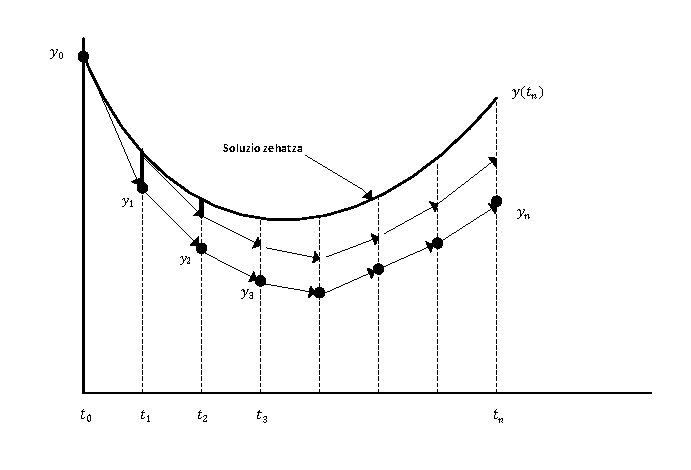
\includegraphics[width=12cm, height=6cm] {ErrorePropagazioa}}
\caption{Errore lokalaren propagazioa. Irudian soluzio zehatza eta hasierako bi balio ezberdinei dagokien zenbakizko soluzioak irudikatu ditugu}
\label{fig:deferror}
\end{figure}     

\item Metodoaren ordena. $h$ urrats luzera finkoko $\phi$ metodoak $p$ ordenakoa dela esaten da, $ge(t)$ errore globala $\mathcal{O}(h^{p})$ ordenekoa bada  $h \rightarrow 0$,
\begin{equation*} 
\label{eq:metordena}
\|y_k-y(t_k)\|=\mathcal{O}(h^{p}), \ \ h \rightarrow 0.
\end{equation*} 
Metodoaren ordena $\mathcal{O}(h^p)$ bada, errore lokala $\mathcal{O}(h^{p+1})$ da.

\end{enumerate}

\item  Metodo simetrikoak.

Urrats bakarreko $\phi_h$ metodoa simetrikoa da, honako baldintza betetzen badu,
\begin{equation*}
\phi_h \circ \phi_{-h}=id,  \ \ \text{edo} \ \ \phi_h=\phi_{-h}^{-1}.
\end{equation*}


\end{enumerate}


\subsubsection*{Euler metodo esplizitua.}

Eulerrek $1768.$ urtean proposatutako zenbakizko metodoa da. Hasierako balio bat emanda $(t_n,y_n)$ eta $h_n>0$ urrats txikirako, $t_{n+1}=t_{n}+h_{n}$ uneko hurbilpena $y_ {n+1} \approx y(t_{n+1})$ era honetan kalkulatuko dugu,  
\begin{equation*}
 \label{eq:202a}
y_{n+1}=y_{n}+h_n f(t_n,y_n).
\end{equation*}
Oinarrizko metodo esplizitua da eta urratsa emateko dagoen konputazio konplexutasuna bakarra, $f$ funtzioaren ebaluazio da. Lehen ordenako metodoa da,
\begin{equation*}
\|y_n-y(t_n)\| \leqslant C h,
\end{equation*}
eta beraz, doitasuna bikoizteko, lan konputazionala bikoiztu behar dugu. Ikusiko dugunez, ordena altuagoko metodoekin, doitasuna handiagoa lortuko dugu, lan konputazional gutxiagorekin. 

\subsubsection*{Euler metodo inplizitua.}

Eulerrek proposatutako beste metodo honek, $y_{n+1}$ hurbilketa, inplizituki definitzen den funtsezko ezaugarria du. $f$ funtzioaren argumentua, aurreko hurbilpenaren ordez hurbilpen berria hartuz definitzen da,
\begin{equation*}
 \label{eq:202b}
y_{n+1}=y_{n}+h_n \ f(t_{n+1},y_{n+1}).
\end{equation*}
Urratsa emateko, ekuazio sistema ez-linealaren soluzioa askatu behar da. Horretarako, iterazio metodo bat aplikatu behar da.

\subsubsection*{Iterazio metodoak}

Laburki, ekuazio sistema ez-linealen soluzioa askatzeko bi iterazio metodo nagusienak azalduko ditugu.

\begin{enumerate}

\item Puntu-finkoaren iterazioa.

Demagun $x=f(x)$ ekuazioa, non $f: {\mathbb{R}}^n  \longrightarrow {\mathbb{R}}^n$ eta  $x^{[0]} \in \mathbb{R}^n$ soluzioaren hasierako hurbilpen bat emanda, puntu-finkoaren iterazioa era honetan definitzen da,
\begin{equation*}
 x^{[k+1]}=f(x^{[k]}) \, \ \ \ \ \ k=1,2,\dots
\end{equation*}
Iterazioak $x^{\ast}$ soluzioarengana konbergitu dezake.

Eta  Euler metodo inplizituaren ekuazio ez-lineala askatzeko, $y_{n+1}^{[0]}$ balioa finkatuta, puntu-finkoaren iterazioa era honetan aplikatuko dugu, 
\begin{equation*}
y_{n+1}^{[k+1]}=y_{n}+h_n \ f(t_{n+1},y_{n+1}^{[k]}), \ \ \ \ \ k=1,2,\dots
\end{equation*}  

\item Newtonen iterazioa.

Demagun $f(x)=0$ ekuazioa askatzeko, non $f: \  {\mathbb{R}}^n \ \longrightarrow {\mathbb{R}}^n$ eta  $x^{[0]} \in \mathbb{R}^n$ soluzioaren hasierako hurbilpen bat emanda, Newtonen iterazioa era honetan definitzen da,
\begin{equation*}
 x^{[k+1]}=x^{[k]}-\frac{f(x^{[k]})}{f`(x^{[k]})} \, \ \ \ \ \ k=1,2,\dots
\end{equation*}

Eta Euler metodo inplizituaren ekuazio ez-lineala askatzeko, $k=1,2,\dots$ iterazioetarako,
\begin{enumerate}
\item $r_{n+1}^{[k]}=y_{n+1}^{[k]}-y_n-h_n \ f(t_{n+1},y_{n+1}^{[k]})$,

\item Askatu $\triangle y_{n+1}^{[k]}$,

$(\triangle y_{n+1}^{[k]} - h_n \ J_n \ \triangle y_{n+1}^{[k]}) =- r_{n+1}^{[k]}$,

\item $y_{n+1}^{[k+1]} = y_{n+1}^{[k]}+ \triangle y_{n+1}^{[k]}$.
\end{enumerate}
non $J_n \approx \frac{\partial f}{\partial y} (t_n, y_n)$ hurbilpen bat den.

\end{enumerate}

Urratsaren konputazioa konplexutasuna, metodo esplizitua baino nabarmen handiagoa da: metodo honetan, iterazio bakoitzean Jacobiarraren ebaluazioa, ekuazio sistema lineala askatu eta $f$ funtzioaren ebaluazioa kalkulatu behar dira.

Iterazio metodoaren konbergentzia abiadura. $\{x^{[0]},x^{[1]},\dots,x^{[k]}\}$, $x^{\ast}$ soluziorantz konbergitzen duen bektore seriea bada, errorea $e^{[n]}=x^{[*]}-x^{[n]}, \ n=1,2,\dots$ izendatuko dugu. Konbergentzia $p$ ordenakoa dela esaten dugu honakoa betetzen dada,
\begin{equation*}
\lim\limits_{n\rightarrow \inf} \frac{\|e^{[n+1]}\|}{\|e^{[n]}\|^p}= C \ne 0.
\end{equation*}

Puntu-finkoaren iterazioak konbergentzia lineala ($p=1$) eta Newtonen iterazioak koadratikoa ($p=2$) du. Konbergentzia koadratikoa izatea oso interesgarria da, iterazio bakoitzean soluzioaren digitu hamartar zuzenen kopurua bikoizten ditugulako. Konbergentzia linealean, ordea, iterazio bakoitzean digitu hamartar kopuru finkoa hobetzen dugu. 
  
\subsubsection*{Problema zurruna.}

Konputazio konplexutasun handiagoa izan arren, problema batzuetan metodo inplizituak, esplizituak aplikatzea baino egokiago izan daiteke, eta hori erakusteko Germund Dahlquist-en ($1963$) adibidea azalduko dugu,
\begin{equation}
 \label{eq:202c}
\dot y=\lambda y,
\end{equation} 
non $\lambda$ balio absolutuan handia eta negatiboa den. Problema honen soluzio analitikoa ezaguna da, $y(t)=e^{(t-t_0)\lambda}$, eta $t \rightarrow \infty$ doanean, soluzioa zerorantz gerturatzen da. Metodo inplizituaren bidezko zenbakizko soluzioa zerorantz gerturatzen da $h>0$ guztietarako,
\begin{equation*}
y_n^{impl}=(1-h\lambda)^{-n} y_0,
\end{equation*}    
eta aldiz, metodo esplizituaren bidezkoa,
\begin{equation*}
y_n^{expl}=(1+h\lambda)^{n} y_0,
\end{equation*}    
zerorantz gerturatuko da soilik $h$ oso balio txikitarako, non $|1+h\lambda|<1$ izan behar duen. Beraz, problema honetan $\lambda$ balio absolutuan handia  eta negatiboa definitu dugunez (adibidez $\lambda=-10^{10}$), Euler esplizituan $h$ urrats tamaina oso txikia erabili behar dugu.    

Euler inplizitua, Euler esplizitua baino eraginkorra den ekuazio diferentzialei problema \emph{zurrunak} (\emph{stiff}) esaten zaie \cite{Hairer2006}. Problema \emph{zurrunen} artean problema garrantzitsuak ditugu, esaterako eskala anitzeko sistemak. 

 

\subsection{Sistema-Hamiltondarrak.}

 
Hamiltondar sistemak \cite{SSerna2015}, ekuazio diferentzial mota garrantzitsu bat dira. $H(p,q)$ funtzio leunari dagokion \emph{Hamiltondar sistema} osatzen duten $2d$ ekuazio diferentzialak, era honetan definitzen dira,
\begin{align*}
\label{eq:212}
\frac{d}{dt} \ {p}^i & =-\frac{\partial H }{\partial q^i} (p,q), \\
\frac{d}{dt} \ {q}^i & =+\frac{\partial H}{\partial p^i} (p,q), \ \ \ \ i=1,\dots,d,
\end{align*}
non $H: {\mathbb{R}}^{2d} \ \longrightarrow {\mathbb{R}}$  den eta  $p=[p^1, \dots , p^d]^T$, $q=[q^1, \dots , q^d]^T$ domeinuaren aldagaiak diren. Egoera aldagaien bektoreen $d$ dimentsioari, sistemaren \emph{askatasun maila} esaten zaio. $H(p,q)$ funtzioari \emph{Hamiltondarra} deritzo, eta sistemaren energia adierazten du. Energia, integrazioan zehar konstante mantentzen da,
\begin{equation*}
\label{eq:212b}
H(p(t),q(t))=const.
\end{equation*}

Beste notazio laburtu hau ere erabili ohi da,
\begin{equation*}
 \label{eq:213}
\dot{y}=J^{-1}\triangledown H(y),
\end{equation*}

non $y=(p,q)$, $\triangledown H=(\partial H/\partial p^1,\dots,\partial H/\partial p^d; \partial H/\partial q^1,\dots,\partial H/\partial q^d)$ eta

\begin{equation*}
 J=\left(\begin{array}{cc}
   \ 0_{dxd} & \ I_{dxd} \\
    -I_{dxd} & \ 0_{dxd} \\
\end{array}\right), \ \ \ 
I_{d \times d}=\left(\begin{array}{cccc}
   \ 1       & 0      & \cdots & 0 \\
   \ 0       & 1      & \cdots & 0 \\
   \ \vdots  & \vdots & \ddots & \vdots \\
   \ 0       & 0 & \cdots & 1 \\
\end{array}\right)  
\end{equation*}


\paragraph*{Hamiltondar banagarriak.} Sistema dinamikoen Hamiltondarrak, maiz egitura berezia du,
\begin{equation*}
H({p},{q})=T(p)+U({q}).
\end{equation*} 

Horien artean, \emph{bigarren ordenako} ekuazio diferentzialak aipatu behar ditugu, zeintzuk Hamiltondar banagarrien kasu partikularra bat diren,  
\begin{equation*}
H(\mathbf(p,q)=\frac{1}{2}p^Tp +U(q),
\end{equation*}
eta dagokien ekuazio diferentzialak hauek diren,
\begin{equation}
\label{eq:biorden}
\dot{p}=-\frac{\partial U(q)}{\partial q}, \ \ \dot{q}=p. 
\end{equation}

\paragraph*{Adibidea.}
\emph{Bi gorputzen} edo \emph{Kepler problema} \cite{Hairer2006}. Planoan elkar erakartzen diren bi gorputzen (adibidez eguzkia eta planeta bat) mugimendua kalkulatzeko, horietako gorputz baten kokapena koordenatu sistemaren jatorria kontsideratuko dugu eta beste gorputzaren kokapenaren koordenatuak $q=(q_1,q_2)$ izendatuko ditugu. 

Funtzio Hamiltondarra hauxe da,
\begin{equation*}
H(p_1,p_2,q_1,q_2)=\frac{1}{2}(p_1^2+p_2^2)-\frac{1}{\sqrt{q_1^2+q_2^2}}.
\end{equation*}

Dagozkion ekuazio diferentzialak,
\begin{align*}
\dot{p}_1 &= -\frac{q_1}{(q_1^2+q_2^2)^{3/2}}, \ \, \dot{p}_2= -\frac{q_2}{(q_1^2+q_2^2)^{3/2}}, \\
\dot{q}_i &=p_i, \ \ \ \ \ i=1,2.
\end{align*}

Planetaren mugimendua orbita eliptiko bat da. Honako hasierako balioei dagokien soluzioa zehatza,
\begin{equation*}
q_1(0)=1-e, \ q_2(0)=0, \ p_1(0)=0, \ p_2(0)=\sqrt{ \frac{1+e}{1-e}}, 
\end{equation*}
$e$ ezentrizidadea ($0\le e < 1$)  eta $P=2\pi$ periodoa duen elipsea da. 

\paragraph*{Hamiltondar perturbatuak.} Hamiltondar perturbatuak, honako egitura duten sistemak ditugu,
\begin{equation*}
H=H_A+\epsilon H_B \ \  \text{non} \ \ |H_B|\ll |H_A|.
\end{equation*}

\paragraph*{Adibidea.} Eguzki-sistemaren probleman \cite{Saha1992,Wisdom2006}, Hamiltondarra modu honetan banatu daiteke $H=H_k+H_I$, non alde nagusia $H_K$ planeta bakoitzaren eguzkiaren inguruko mugimendu Kepleriarrari eta $H_I$ aldiz, planeten arteko interakzioek eragiten duten perturbazio txikiari dagokion.   

\subsection{Metodo sinplektikoak.}

Hamiltondar sistemen problemetarako, Euler esplizitua eta Euler inplizitua ez dira zenbakizko metodo egokiak. Problema hauen propietate geometrikoak mantentzen dituzte integratzaile bereziak beharrezkoak dira \cite{JMSanz-Serna1994,SSerna2015b}. Integratzaile hauek, metodo sinplektikoak dira eta abantaila handiena, epe luzeko integrazioetan azaltzen dute.

Metodo sinplektikoen lehen aipamenak, $1950$ hamarkadan kokatu behar dira eta $1980$ hamarkadan, Feng Kang-ek metodo hauen azterketa sakona burutu zuen. Hastapenetako lan monografiko hau \cite{JMSanz-Serna1994} eta ondorengo, azalpen ulergarriak jasotzen dituzten \cite{Hairer2006} eta  \cite{Leimkuhler2004} lanak aipatu daitezke.    

\begin{figure}[h!]
\centering
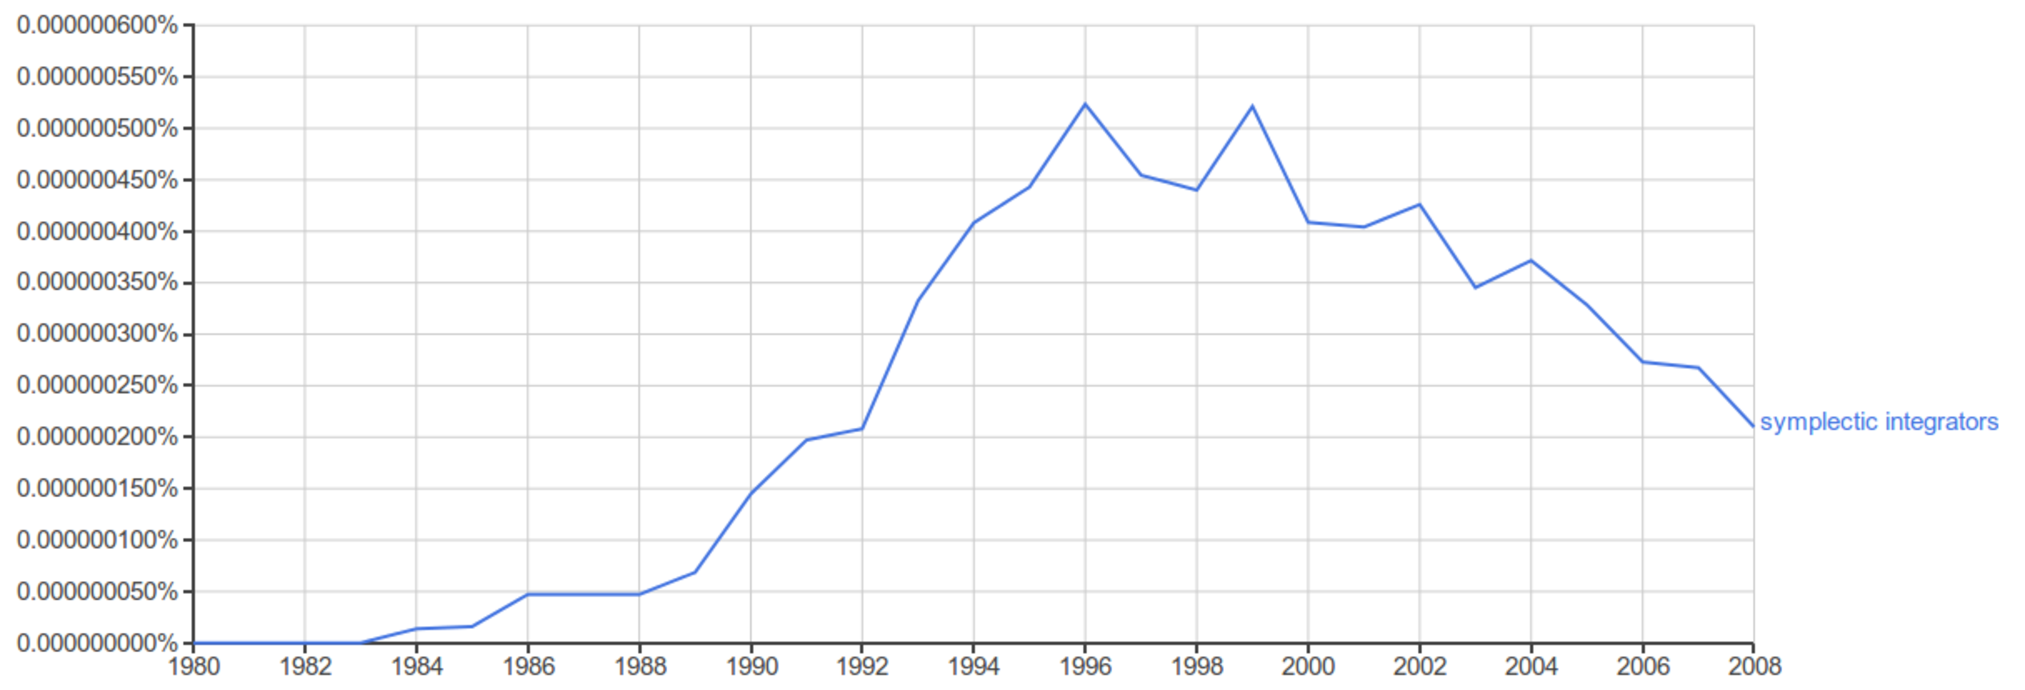
\includegraphics[width=1.0\textwidth]{NgramSymplectic}
\caption{ \small Google-n ngram aplikazioan "symplectic integrators" gaiaren bilaketan lortutako irudia.}
\label{fig:NgramSymplectic}
\end{figure}

\paragraph*{Adibidea.} Metodo sinplektikoen abantaila azaltzeko, penduluaren problema aukeratu dugu \cite{Hairer2015a}. Penduluaren problemaren (masa $m=1$, $l=1$ luzerako makila eta $g=1$ grabitazioa) $d=1$ askatasuneko sistema Hamiltondarra,
\begin{equation}
H(p,q)= \frac{p^2}{2}- cos (q),
\end{equation}

eta ekuazio diferentzialak,
\begin{equation}
\label{eq:pendulua}
\dot{p}= -sin (q), \ \ \dot{q}=p.
\end{equation}

\ref{fig:pendulua} irudian ikusi daitekeenez, Euler esplizitu eta inplizituaren konportamendu kualitatiboki okerra da. Era honetan definitzen den Euler sinplektikoa \cite{Hairer2006} ordea, 
\begin{align}
\label{eq:eulersin}
\begin{split}
p_{n+1} & =p_n-h \ \frac{\partial H }{\partial q} (p_{n+1},q_{n}), \\
q_{n+1} & =q_n+h \ \frac{\partial H}{\partial p} (p_{n+1},q_{n}),
\end{split}
\end{align}
sistemaren energia kontserbatzen du integrazio luzean zehar.


\begin{figure}[h!]
\centering
\begin{tabular}{c c}
\subfloat[Pendulua.]{
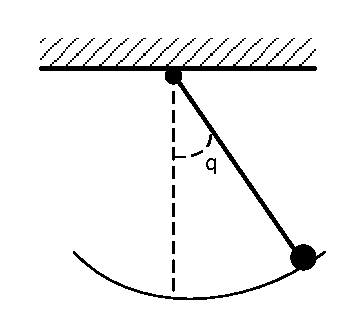
\includegraphics[width=.30\textwidth]{PenduluArrunta}
}
&
\subfloat[Integrazioa.]{
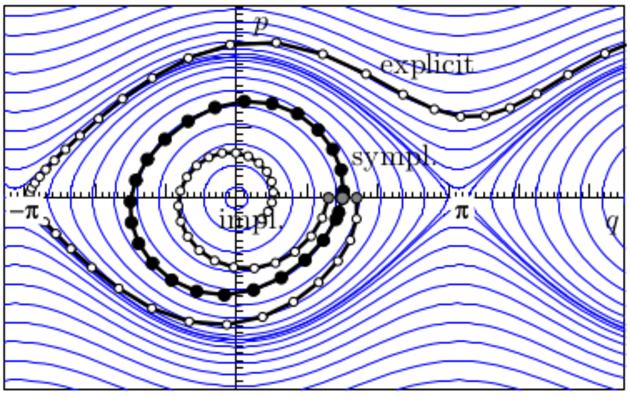
\includegraphics[width=.40\textwidth]{pcam-irudia}
}
\end{tabular}
\caption{ \small Pendulu problemaren hiru zenbakizko metodoen zenbakizko soluzioak irudikatu ditugu. Hiruretan urrats luzera berdina $h=0.3$ baina bakoitza hasierako balio ezberdinarekin. Euler esplizitua $(p(0),q(0))=(0,1.7)$; Euler sinplektikoa $(p(0),q(0))=(0,1.5)$; Euler inplizitua $(p(0),q(0))=(0,1.3)$.}
\label{fig:pendulua}
\end{figure}


Metodo sinplektikoak bi taldeetan banatuko ditugu: metodo sinplektiko inplizituak eta  esplizituak. Lehenengo taldean,  Runge-Kutta metodo inplizituak (Gauss kolokazio metodoak) ditugu. Metodo hauek zenbakizko metodo estandarrak dira eta ekuazio diferentzial orokorrei aplika daitezke. Bigarren taldean, konposizioan eta splitting-ean oinarritutako metodoak ditugu. Azken talde honetako metodoak, bakarrik Hamiltondar sistemei aplika daitezke eta gainera, Hamiltondarrak banagarria izan behar du. Konposizio eta splitting metodoak oso eraginkorrak dira.   


\subsubsection*{Metodo sinplektikoen propietateak.}

Funtsezkoa da, integratzaile sinplektiko baten bidez lortutako $H$ Hamiltondar sistemaren zenbakizko soluzioa, perturbatutako beste Hamiltondar $\widetilde{H}$ baten soluzio zehatza gisa ulertzea \cite{SSerna2015b}. Kontutan hartu behar da, zenbakizko integrazioak eragiten dituen perturbazio hauek, sistema dinamiko baten $H$ Hamiltondar eredua eraikitzerakoan, hartzen  diren hurbilpenek edo datu ez ziurrek eragiten duten baino errore maila txikiagoa suposatzen dutela.    
 

\paragraph{Adibidea.}
Demagun, askatasun maila bakarra duen sistema Hamiltondar banagarria $H=T(p)+V(q)$, Euler metodo sinplektikoaren (\ref{eq:eulersin}) bidez integratzen dugula.  $(p_n,q_n)$ zenbakizko soluzioak, integratu nahi dugun $S$ Hamiltondar sistemaren $(p(t_n),q(t_n))$ soluzio zehatza hurbiltzen du.  Modu honetan, benetako fluxua $\varphi_h^H$ eta zenbakizko integrazioa $\phi_h^H$ izendatzen baditugu,
\begin{align*}
&(p_{n+1},q_{n+1}) =\phi_h^H(p_n,q_n), \\
&(p(t_{n+1}),q(t_{n+1})) =\varphi_h^H(p(t_n),q(t_n)), 
\end{align*} 
eta Euler sinplektikoa $p=1$ ordenako metodoa denez,
\begin{equation*}
\phi_h^H(p_n,q_n)-\varphi_h^H(p(t_n),q(t_n))= \mathcal{O}(h^2).
\end{equation*}    

\paragraph*{}Defini daiteke beste $S_2$ Hamiltondar sistema bat, zeinekin Euler sinplektikoa bigarren ordenako den? Hau da, $(p_n,q_n)$ zenbakizko soluzioa, $S$ soluziotik baino gertuago dagoen $S_2$ sistema? 
\begin{align*}
\phi_h^{\widetilde{H}}(p_n,q_n)-\varphi_h^{\widetilde{H}}(p(t_n),q(t_n))= \mathcal{O}(h^3).
\end{align*}

Taylor seriea garatuz, lortuko dugu $S_2$ sistema  ($f=-\partial H/\partial q$, $g=\partial H/\partial p$),
\begin{align*}
\frac{d}{dt} p &= f(q)+ \frac{h}{2} g(p) f'(q),\\
\frac{d}{dt} q &= g(p)- \frac{h}{2} g'(p) f(q),
\end{align*} 
non honako Hamiltondarrari dagokion,
\begin{align*}
\widetilde{H}_2=T(p)+V(q)+\frac{h}{2} T'(p) V'(q) = H+\mathcal{O}(h).
\end{align*}

\ref{fig:MetSinplektikoa} irudian, pendulu problemaren (\ref{eq:pendulua}) hasierako balio hauei ($p(0)=0, \ q(0)=2$) dagokien integrazioa erakutsi dugu. Izarrak, $h=0.5$ urratsari dagokion zenbakizko soluzioa da. $H=const$~puntuko lerroak, penduluaren benetako soluzioa irudikatzen du.  $\widetilde{H}_2=const$~marra lerroak, perturbatutako Hamiltondar sistemaren soluzioa irudikatzen du. Zenbakizko soluzioaren eta perturbatutako Hamiltondar sistemaren ibilbideak bat datozela ikusi daiteke. 

\begin{figure}[h!]
\centering
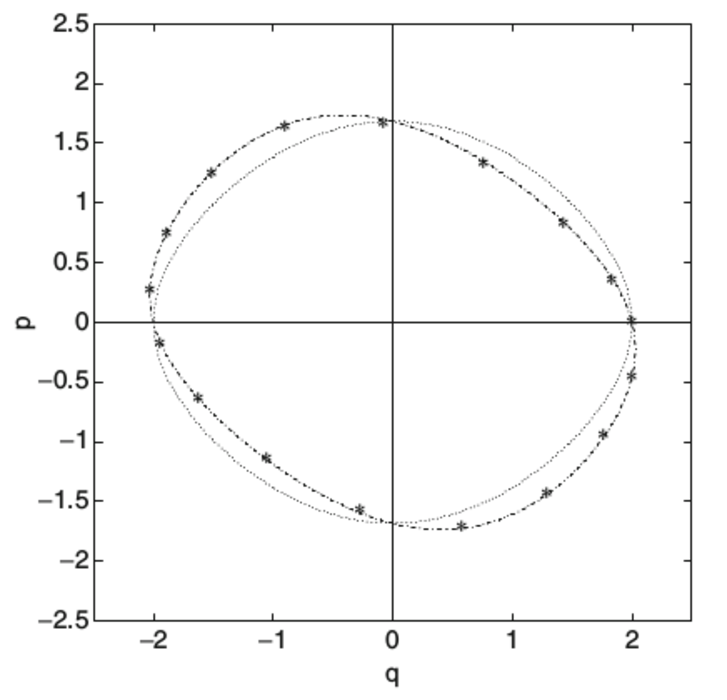
\includegraphics[width=.40\textwidth]{MetSinplektikoa}
\caption{ \small Penduluaren problema: zenbakizko soluzioa (izarrak), benetako soluzioa (puntu lerroak) and perturbatutako soluzioa (marra lerroak) \cite{SSerna2015b}}
\label{fig:MetSinplektikoa}
\end{figure}

Kasu orokorra, posible da $S_p$ Hamiltondar sistema perturbatua eraikitzea, zeinekin Euler sinplektikoa $p$ ordenakoa den. Beraz, konklusio gisa esango dugu, Hamiltondar sistema bati aplikatzen diogun metodo sinplektikoaren zenbakizko soluzioa, perturbatutako Hamiltondar sistema baten soluzio ia zehatza kontsideratu behar dugula. 

Sarrera hau bukatzeko, metodo sinplektikoen propietate nagusienak azpimarratuko ditugu \cite{Hairer2006,JMSanz-Serna1994}.
\begin{enumerate}

\item Metodo sinplektikoek, energia oso ondo kontserbatzen dute.

Sistema Hamiltondarren $H(p,q)$ funtzio leunari, sistemaren energia deitzen zaio. Soluzio zehatzak, energia konstantea mantentzen du,
\begin{equation*}
H(p(t),q(t))=Const.
\end{equation*}
Zenbakizko soluzioak ordea, ez du $H(p_n,q_n)$  konstante mantentzen. Integrazio metodoa sinplektikoa bada, aritmetika zehatzarekin energia errorea bornatua mantentzen da eta drift-arik gabe. Koma-higikorreko aritmetikarekin, biribiltze errorearen eraginez energia errorea denboraren erro karratuaren arabera hasiko da,
\begin{equation*}
\frac{H(p_n,q_n)-H(p_0,q_0)}{H(p_0,q_0)}=k \ \sqrt{t_n}.
\end{equation*}
non $k\in \mathbb{R}$ den.

\item Errore propagazio lineala.

Gehienetan, $p$ eta $q$ egoera aldagaien errorea $\mathcal{O}(h^p)$ da eta hazkundea lineala. Oro har, integratzaile arruntek errore hazkunde koadratikoa dute eta ondorioz, integrazio luzeetan konportamendu txarra azaltzen dute.

\item Metodo sinplektiko garrantzitsuenak simetrikoak dira.

\item Urrats luzera finkoa erabili behar da izaera sinplektikoa ez galtzeko \cite{JMSanz-Serna1994}.  Metodo gehienak eraginkorrak izateko, errore estimazio baten arabera integrazioan zehar urrats luzera egokitzen dute. Soluzioaren aldaketa azkarrak gertatzen diren uneetarako urratsa txikia, eta aldiz, urratsa handia soluzioa leuna den uneetarako.   

\end{enumerate} 

\section{Runge-Kutta metodo sinplektikoak.}


1988. urtean, Sanz-Sernak \cite{JMSanz-Serna1994} \emph{Gauss metodoa} sinplektikoa zela ohartu zen, s-ataleko ordena altueneko metodoa ($p=2s$) izanik. Runge-Kutta metodo inplizitua da eta hainbat propietate interesgarri ditu. 

\subsection{Runge-Kutta metodoak.}

Runge-Kutta metodoak \cite{Hairer2006}, urrats bakarreko ekuazio diferentzial arrunten zenbakizko integrazio metodoak dira.  $b_{i}$, $a_{ij}$ eta $c_i=\sum\limits_{j=1}^{s} a_{ij} \ (1 \leq i,j \leq s)$ koefiziente errealek s-ataleko Runge-Kutta metodoa definitzen dute eta \emph{Butcher} izeneko taulan moduan laburtu ohi dira, 
\begin{equation}
\label{eq:btchtaula}
\begin{array}{c|c}
  c & A  \\
  \hline
   &  b^T\\
\end{array}, \ \ \ \ \ \ \ \ \ \ \ \
\begin{array}{c|cccc}
  \ c_1 &  a_{11} & a_{12} & \dots & a_{1s}\\
  \ c_2 &  a_{21} & a_{22} & \dots &a_{2s}\\
  \ \vdots & \vdots & \vdots & \ddots & \vdots \\
  \ c_s & a_{s1} & a_{s2} & \dots & a_{ss}\\
  \hline
  \  & b_{1} & b_{2} & \dots & b_{s}\\
\end{array}
\end{equation}

Hasierako baliodun problemaren (\ref{eq:ivp})  $y_n \approx y(t_n)$ soluzioaren hurbilpena era honetan kalkulatzen da,
\begin{equation}  
y_{n+1}=y_n+h\sum^s_{i=1}{b_i \ f(t_n+c_ih,Y_{n,i})\ \ },\
\end{equation} 

non $Y_{n,i}$ atalak era honetan definitzen diren,
\begin{equation}
Y_{n,i}=y_n+\ h\ \sum^s_{j=1}{a_{ij}\ f(t_n+c_jh,Y_{n,j})}\ \ \ \ \ i=1 ,\dots, s.\
\end{equation} 

Bi idei dago, Runge-Kutta metodoaren oinarrian. Lehenik, integrala
\begin{equation*}
y(t_0+h)=y(t_0)+h \int_{0}^{1} \dot{y}(t_0+\theta h) d\theta,
\end{equation*} 
non $\dot{y}(t)=f(t,y(t))$ den, $b_i$ pisuak eta $c_i$ nodoak dituen hurrengo koadratura formularekin hurbiltzen da,
\begin{equation*}
 y_{1}=y_0+h\sum^s_{i=1}{b_i \ f(t_0+c_ih,Y_{i})}.
\end{equation*}

Bigarrenik, $Y_{i} \approx y(t_0+c_ih)$~atalen $0$ eta $c_i$ arteko integrala, beste koadratura formularekin hurbiltzen da,
\begin{equation*}
Y_{n,i}=y_0+h \sum_{j=1}^{s} a_{ij} \ f(t_0+c_ih,Y_{i}).
\end{equation*}

\subsubsection*{Metodo esplizituak (ERK) eta inplizituak (IRK).}
Runge-Kutta bi talde nagusitan bereiz ditzakegu: esplizituak (\emph {ERK}) non $\forall i\ge j, \ a_{ij}=0 $ eta inplizituak (\emph {IRK}) non $\exists i \ge j \ , a_{ij} \ne 0$ . 


\begin{enumerate}
\item \emph{ERK} metodoaren adibidea.

$s=4$ ataletako ERK metodo klasikoa era honetan definitzen da, 
\begin{equation*}
\begin{array}{c|cccc}
  \ 0   &    &    &     &      \\
  \ 1/2 & 1/2 &   &     &      \\
  \ 1/2 & 0   & 1/2  &  &      \\
  \ 1   & 0   & 0    &  1   &   \\
  \hline
  \     & 1/6 & 2/6  &  2/6 & 1/6 \\
  \end{array} \\
\end{equation*}

$Y_{n,i}$ atalak, esplizituki kalkula daitezke,
\begin{equation*}
Y_{n,i}=y_n+\ h\ \sum^{i-1}_{j=1}{a_{ij}\ f(t_n+c_jh,Y_{n,j})}\ \ \ \ \ i=1 ,\dots, s.
\end{equation*}  

\item \emph{IRK} metodoaren adibidea.

Honakoa da, $s=1$ ataleko \emph{Implicit Midpoint method}-aren definizioa, 
\begin{equation*}
\begin{array}{c|c}
  \ 1/2 &  1/2\\
  \hline
  \     & 1 \\
\end{array} \\
\end{equation*}

$Y_{n,1}$ atala inplizituki definituta dago, eta honako ekuazio ez-lineala ebatzi behar da,
\begin{equation*}
Y_{n,1}=y_n+\ \frac{h}{2} \ f(t_n+\frac{h}{2},Y_{n,1}).
\end{equation*} 

\end{enumerate}

\emph{ERK} lau-ataletako  metodo klasikoa, $p=4$ ordenakoa dugu. Ordena altuko \emph{ERK} metodoak aurkitzea konplexua da,  koefizienteek bete behar dituzten ordena baldintzen kopurua esponentzialki hazten baitira. Esate baterako, ordena altuko \emph {ERK} metodo hauek aurkitu dira:  $s=11$ ataletako $p=8$ ordenako metodoa,  $s=17$ ataletako $p=10$ ordenako metodoa eta  $s=25$ ataletako $p=12$ ordenako metodoa.
 
Ordena altuko \emph{IRK} metodoak, \emph{ERK} metodoak baino modu errazagoan eraiki daitezke.  \emph{Butcher sinplifikazio baldintza} hauen \cite{Butcher2008} arabera definitzen dira,
\begin{align}
B(p) &: \ \ \ \sum\limits_{i=1}^{s} b_ic_i^{q-1} =\frac{1}{q}, \ \ & q=1,\dots,p. \\
C(\eta) &: \ \ \ \sum\limits_{j=1}^{s} a_{ij}c_j^{q-1}  =\frac{c_i^q}{q},& \ \ i=1,\dots,s, \ q=1,\dots,\eta.\\
D(\zeta) &:  \ \ \ \sum\limits_{i=1}^{s}  b_i c_i^{q-1}  a_{ij} = \frac{b_j}{q} (1-c_j^q),&  \ j=1,\dots,s, \  q=1,\dots,\zeta.
\end{align}

\ref{tab:irk} taulan, \emph{IRK} metodo nagusienak laburtu ditugu. 
\begin{table}[h]
\centering
\caption{Runge-Kutta metodo inplizituak.}
\label{tab:irk}       % Give a unique label
\begin{tabular}{ l l l l c } 
 \hline
 \\
 Metodoa          &  Baldintzak             &                        &                 & Ordena \\
 \\
 \hline
 Gauss            &  $B(2s)$                & $C(s)$                 & $D(s)$          & $2s$    \\
% \hline
 Radau IA         &  $B(2s-1)$              & $C(s-1)$               & $D(s)$          & $2s-1$  \\
% \hline 
 Radau IIA        &  $B(2s-1)$             & $C(s)$                  & $D(s-1)$        & $2s-1$  \\
% \hline 
 Lobatto IIIA     &  $B(2s-2)$              & $C(s)$                 & $D(s-2)$        & $2s-2$  \\
% \hline
 Lobatto IIIB     &  $B(2s-2)$              & $C(s-2)$               & $D(s)$          & $2s-2$  \\
% \hline 
 Lobatto IIIC     &  $B(2s-2)$              & $C(s-1)$               & $D(s-1)$        & $2s-2$  \\
  \hline
 \end{tabular}
\end{table}

\subsubsection*{Sinplektikotasuna.}

Sanz-Sernak  \cite{JMSanz-Serna1994} Runge-Kutta metodoa sinplektikoa izateko baldintza nahikoa eta beharrezkoa,
\begin{equation}
\label{eq:simplektik}
b_{i}a_{ij}+b_{j}a_{ji}-b_{i}b_{j}=0, \ \ 1 \leqslant i,j \leqslant s,
\end{equation}
dela frogatu zuen.

Baldintza honen arabera, Runge-Kutta metodo esplizituak, sinplektikoak ezin daitezkeela izan ondorioztatu daiteke. Bestalde, 1988. urtean, Sanz-Sernak \emph{Gauss metodoa} sinplektikoa zela ohartu zen. 

\subsection{Gauss metodoa.}

Gauss metodoa beste \emph{IRK} metodoekin alderatuta, bi ezaugarri bereizten ditu:  Runge-Kutta metodo sinplektiko bakarra eta $s$-ataletako ordena altueneko ($p=2s$) IRK metodoa da. 

Kolokazio metodoak, zenbakizko integrazio metodo garrantzitsuak dira. Gauss metodoa kolokazio metodoa da eta jarraian, ikuspegi honetatik definituko dugu. 

\subsubsection*{Kolokazio metodoak.}

$c_1,c_2,\dots,c_s \ \ (0\leq c_i \leq 1)$ nodoetan oinarritutako kolokazio metodoak, $s$-mailako $u(t)$  \emph{polinomioa} definitzen du. Polinomioak honakoa betetzen du,
\begin{align*}
&u(t_0) =y_0, \\
&\dot{u}(t_0+c_ih) =f(t_0+c_i h, u(t_0+c_i h)), \ \ i=1,\dots,s.
\end{align*}
eta soluzioa 
\begin{equation*}
y_1=u(t_0+h)\approx y(t_0+h).
\end{equation*} 

Kolokazio metodoen zenbakizko soluzioa, diskretizazio puntuetan ez ezik, interpolazio polinomio batek modu jarraian emandako soluzioa adierazten du. 

Guillou-k eta Soule-k ($1969$), Wright-ek ($1970$) \cite{Hairer2006} kolokazio metodoaren definizioa eta modu honetan kalkulatutako s-ataleko Runge-Kutta metodoa baliokideak direla, frogatu zuten.
\begin{equation}
a_{ij}=\int_{0}^{c_i} l_j(\tau) \ d\tau, \ \ b_i=\int_{0}^{1} l_i(\tau) \ d\tau
\end{equation}

non $l_i(\tau)$ Lagrangiar polinomioa dugu $l_i(\tau)=\prod_{l\neq i} \frac{(\tau-c_l)}{(c_i-c_l)}$.

Gauss nodoak. Gauss metodoak $c_i$ ($1 \leq i \leq s)$ koefizienteak "sth shifted Legendre" polinomioaren zeroak aukeratuz,
\begin{equation*}
\frac{d^s}{dx^s} \big(x^s(x-1)^s \big),
\end{equation*} 
Nodo hauetan oinarritutako Runge-Kutta metodoa $p=2s$ ordena du.

\subsubsection*{Gauss metodoaren koefizienteak.}

$s=1$, $s=2$ eta $s=3$ ataletako, Gauss metodoaren \cite{Hairer2006} \emph{Butcher} koefiziente taulak \cite{Hairer2006} zehaztuko ditugu,
\begin{equation*}
\begin{array}{c|c}
  \frac{1}{2} & \ \frac{1}{2} \\
  \\
  \hline
   & 1 \\
\end{array} \ \ \ ,  \ \ \ \ \ \ \ \ \
\begin{array}{c|c c}
  \frac{1}{2}-\frac{\sqrt{3}}{6} & \ \frac{1}{4} & \ \frac{1}{4}-\frac{\sqrt{3}}{6} \\
  \\
  \frac{1}{2}+\frac{\sqrt{3}}{6} & \ \frac{1}{4}+\frac{\sqrt{3}}{6} & \ \frac{1}{4} \\
  \\
  \hline
         &  \frac{1}{2} & \ \frac{1}{2} \\
\end{array},
\end{equation*}

\begin{equation*}
\begin{array}{c|c c c}
  \frac{1}{2}-\frac{\sqrt{15}}{10} & \ \frac{5}{36} & \ \frac{2}{9}-\frac{\sqrt{15}}{15} & \ \frac{5}{36}-\frac{\sqrt{15}}{30} \\
  \\
  \frac{1}{2}   & \ \frac{5}{36}+\frac{\sqrt{15}}{24} & \ \frac{2}{9} & \ \frac{5}{36}-\frac{\sqrt{15}}{24} \\
  \\
  \frac{1}{2}+\frac{\sqrt{15}}{10}   & \ \frac{5}{36}+\frac{\sqrt{15}}{30} & \ \frac{2}{9}+\frac{\sqrt{15}}{15} & \ \frac{5}{36} \\
  \\
  \hline
  & \frac{5}{18} & \ \frac{4}{9} & \ \frac{5}{18}
\end{array}.
\end{equation*}

\subsubsection*{Gauss metodoaren propietateak.}

Jarraian, Gauss metodoaren ezaugarri orokorrak azalduko ditugu:  
\begin{enumerate}
\item{Metodo sinplektikoa (\ref{eq:simplektik})}. 
 
\item{Metodo simetrikoa.}

Runge-Kutta metodoa, simetrikoa izateko baldintzak hauek dira,
\begin{align*}
\label {eq:2}
 b_{i} &= b_{\sigma(i)} ,\ \  c_{\sigma(i)}= 1-c_{i}, \\
 b_{j} &= a_{\sigma(i),\sigma(j)}+a_{i,j}, \ \  i=1,2,\dots \lfloor s/2\rfloor
 \end{align*} 
non $\sigma(i)=s+1-i$.

Kolokazio metodo simetrikoetan, $c_i$ balioak integrazio urratsaren erdigunearekiko simetrikoak dira (ikus \ref{fig:simetrikoa} irudia  ).  
 \begin{figure}[h]
 \centering
 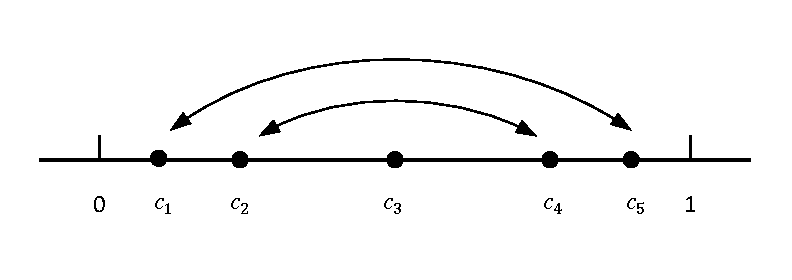
\includegraphics[width=.60\textwidth]{Simetria}
 \caption{ \small Kolokazio metodoen simetria.}
 \label{fig:simetrikoa}
 \end{figure}
 
\item{Ordena altuko metodoa.}
Edozein ordenako Gauss metodoa eraiki daiteke. Doitasun handiko konputazioetarako ordena altuko metodoak beharrezkoak dira: doitasun bikoitzeko aritmetikan ($u\approx10^{-16}$) ~$p\ge8$ ordenako metodoak gomendagarriak dira eta doitasun laukoitzeko aritmetikan ($u\approx10^{-35}$) ordena altuagoko metodoak beharrezkoak dira.  

\item{Metodo orokorra.}
Gauss metodoa edozein ekuazio diferentzialari aplika daiteke. Sistema Hamiltondarren problemetan, ez du zertan banagarria izan behar.

\item{Paralelizagarria.}
Ekuazio diferentzial garestiak ditugunean, $s$-ataletako funtzio konputazioak ($f(Y_i), \ i=1,\dots,s$) paraleloan kalkula daitezke.  

\item{Kolokazio metodoa.}
Zenbakizko soluzioa diskretizazio puntuetan ez ezik, integrazio tarte bakoitzean polinomio interpolatzaile batek modu jarraian emandako soluzioa adierazten du.

\item{A-stability and B-stability.}
A-stable methods have a central role in the numerical solution of stiff problems and Gauss methods are likely candidates.
  
\end{enumerate}

      
\subsection{IRK inplementazioa.}

\subsubsection*{IRK algoritmoa.}

Jarraian, \emph{IRK} metodoaren inplementazioaren \ref{alg:IRK1} algoritmo orokorraren laguntzarekin, inplementazioaren ezaugarri orokor batzuk deskribatuko ditugu.

\begin{algorithm}[H]
 \BlankLine
  $y_0=y(t_0)$\;
 \BlankLine
  \For{$n\leftarrow 0$ \KwTo ($endstep-1$)}
  {
   \BlankLine
   $k=0$\;
   \text{Hasieratu}  $Y_{n,i}^{[0]} \ \ , \ \ i=1,\dots,s $\;
    \BlankLine
   \While{ (konbergentzia lortu)}
   {
    \BlankLine
    $k=k+1$\; 
    $F_{n,i}^{[k]}=f(t_n+c_ih,Y_{n,i}^{[k-1]}) $\;
    \text{Askatu} ($Y_{n,i}^{[k]}=y_{n}+ h \ \sum\limits_{j=1}^{s} a_{ij} F_{n,j}^{[k]}$) \; 
    $\text{konbergentzia} \leftarrow \text{GeratzeErizpidea}(Y^{[k]},Y^{[k-1]}) $\; 
   }
   \BlankLine
    $\delta_n=h \ \sum\limits_{i=1}^{s} b_i F_{n,i}$\;
    $y_{n+1}=y_{n}+ \delta_n $\;
   \BlankLine
 }
 \caption{IRK Algoritmo orokorra}
 \label{alg:IRK1}
\end{algorithm}


\subsubsection*{Atalen hasieraketa.}
\label{ss:2.2.3.2}

Atalen hasieraketa egokia definitu behar da. Aukera sinpleena $Y_{n,i}^{[0]}=y_{n}$ hasieratzea da, baina aurreko urratseko atalen informazioa erabiliz hurbilketa hobea lortu daiteke \cite{Hairer2006}. Aurreko urratseko atalen interpolazio polinomio bidezko hasieraketa era honetan adierazi dezakegu,
\begin{equation*}
Y_{n,i}^{[0]}=g(Y_{n-1,i}) \ , \ i=1, \dots, s. 
\end{equation*}

Aurreko urratseko $Y_{n-1,i}$~atalak eta $(t_{n-1}+h,y_{n})$ zenbakizko soluzioa ezagututa, interpolazio polinomio bidez, urrats berriaren atalen hasieraketa  $Y_{n,i}^{[0]}$ kalkulatuko dugu (\ref{fig:AtalHasieraketa} Irudia). 
\begin{figure}[h!]
\centerline{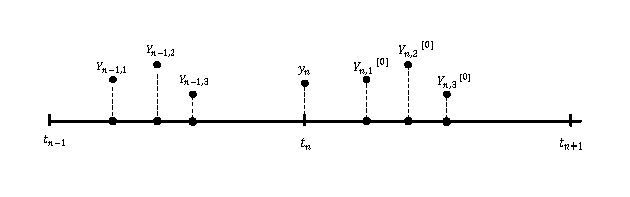
\includegraphics[width=14cm, height=4cm] {YiAtalenHasieraketa}}
\caption{Interpolazioa.}
\label{fig:AtalHasieraketa}
\end{figure}

\begin{enumerate}
\item ($n-1$). urratsaren informazioa.
\begin{align*}
\left \{ \begin{array}{c}
Y_{n-1,i} =y_{n-1}+h \sum\limits_{j=1}^{s} a_{ij} f(Y_{n-1,j}),\\
y_n =y_{n-1}+h \sum\limits_{j=1}^{s} b_j f(Y_{n-1,j}),\\
\end{array} \right.
\ \Rightarrow \ \ 
Y_{n-1,i} &=y_n+h \sum\limits_{j=1}^{s} (a_{ij}-b_j) f(Y_{n-1,j}).
\end{align*}

\item Interpolazio polinomioa.
\begin{equation*}
P(t)=  l_1(t) Y_{n-1,1}+\dots+l_s(t) Y_{n-1,s}+l_{s+1}(t) y_n
\end{equation*}
  
non $l_i(t)$ Lagrangiar polinomioa dugun,
\begin{equation*}
 l_i(t)=\prod_{l\neq i,l=1}^{s+1} \frac{(t-(t_{n-1}+hc_l))}{(c_i-c_l)}, \ \ c_{s+1}=1.
\end{equation*}

\item Atalen hasieraketa.
\begin{equation*}
Y_{n,i} \approx Y_{n,i}^{[0]}= P(t_n+hc_i) = y_n+ h \sum\limits_{j=1}^{s} \lambda_{ij}f(Y_{n-1,j}).
\end{equation*}

\end{enumerate}

Modu honetan s-ataletako IRK metodo bakoitzari dagokion, $\lambda_{ij}$ interpolaziorako koefizienteak lortu daitezke (\ref{sec:B1} atala). Interpolazio polinomioaren bidezko hasieraketa, emandako urratsa oso handia eta problema zurruna ez bada, ona izango da,. Era berean aipatu nahi genuke, atal askotako metodoetan (adibidez $s=16$)  interpolaziozko koefizienteen kalkuluan ezabapen arazoak, doitasun handian lan egitera behartzen gaituela interpolaziozko hasieraketa ona izateko.   

Laburta-ren lanean \cite{Laburta1998}, hasieraketa aurreratuei buruzko informazioa aurkitu daiteke.  


\subsubsection*{Iterazio metodoa.}

\emph{IRK} metodoen erronka handiena, ekuazio-sistema ez-linealaren zenbakizko soluzioaren inplementazio eraginkorra da \cite{Hairer2006,SSerna2015b}. Problema ez-zurrunetarako, atalen hasieraketa ($Y_i^{[0]}$) egoki bat duen puntu-finkoaren iterazioa erabil daiteke. Problema zurrunetarako, puntu-finkoaren iterazioak urrats tamaina txikiegia erabiltzea behartuko luke eta ondorioz, Newtonen iterazio sinplifikatua erabili ohi da.  

\begin{enumerate}

\item Puntu-finkoaren iterazioa.

\begin{algorithm}[H]
  \For{ (k=1,2,\dots)}
  {
   $F_{i}^{[k]}=f(t_n+c_ih,Y_i^{[k-1]})$\;
   $Y_{i}^{[k]}=y_{n}+ h \ \sum\limits_{j=1}^{s} a_{ij} F_{j}^{[k]} , \ \  i=1,\dots,s$\; 
  }
 \caption{Puntu-finkoaren iterazioa.}
 \label{alg:rkpf}
\end{algorithm}

Konbergentzia $\|Y^k-Y\|=\mathcal{O}(h) \|Y^{k-1}-Y\|$.


\item Newtonen iterazioa. 

Newton metodoa iterazio bakoitza konputazionalki garestia da. Batetik,  $\frac{\partial f}{\partial y}(t_n+c_ih,Y_i^{[k-1]}), \ i=1,\dots,s$ Jacobiarrak ebaluatu behar dira. Bestetik, s-ataletako IRK metodoa eta  d-dimentsioko ekuazio diferentziala baditugu, $sd \times sd$ matrizearen \emph{LU-deskonposaketa} kalkulatu behar da.    

\begin{algorithm}[H]
  \For{ (k=1,2,\dots)}
  {
   $r_{i}^{[k]}=-Y_i^{[k-1]}+y_n+h \ \sum\limits_{j=1}^{s} a_{ij} f(t_n+c_ih,Y_j^{[k-1]}) $\;
   Askatu $\triangle Y_i^{[k]}$\;
   $\triangle Y_i^{[k]}-h \ \sum\limits_{j=1}^{s} a_{ij} \frac{\partial f}{\partial y}(t_n+c_jh,Y_j^{[k-1]}) \ \triangle Y_j^{[k]}=r_i^{[k]}$\;
   $Y_i^{[k]}=Y_i^{[k-1]}+\triangle Y_i^{[k]}, \ \  i=1,\dots,s$\; 
  }
 \caption{Newton metodoaren iterazioa}
\end{algorithm}

Konbergentzia $\|Y^k-Y\|=\mathcal{O}(h^2) \|Y^{k-1}-Y\|$.

\end{enumerate}

\subsubsection*{Hamiltondar banagarriak (Metodo partizionatuak).}

Era honetako ekuazio diferentzialak, garrantzitsuak dira,
\begin{equation*}
\dot{p}=f(q), \ \ \dot{q}=g(p).
\end{equation*}

Esaterako, Hamiltondar banagarriak $H(q,p)=T(p)+U(q)$ eta bigarren ordenako ekuazio diferentzialak $\ddot{q}=f(q)$ era honetako ekuazio diferentzialen kasu partikularrak dira.

Zenbakizko soluzioa $(p_{n+1},q_{n+1}) \approx (p(t_{n+1}),q(t_{n+1}))$ era honetan kalkulatuko dugu \cite{JMSanz-Serna1994},
\begin{align}
\begin{split}
&p_{n+1}=p_n+ h \sum\limits_{i=1}^{s} b_i \ f(t_n+c_ih,Q_{n,i}),\\
&q_{n+1}=q_n+ h \sum\limits_{i=1}^{s} b_i \ g(t_n+c_ih,P_{n,i}),
\end{split}
\end{align}

non $P_{n,i},Q_{n,i} \ i=1,\dots,s$ atalak, honako ekuazio sistema definitutakoak diren, 
\begin{align}
\begin{split}
&P_{n,i} =p_n+ h \sum\limits_{j=1}^{s} a_{ij} \ f(t_n+c_jh,Q_{n,j}), \\
&Q_{n,i} =q_n+ h \sum\limits_{j=1}^{s} a_{ij} \ g(t_n+c_jh,P_{n,j}).
\end{split}
\end{align}

Problema hauetan,  funtsean puntu-finkoaren iterazioa (\ref{alg:rkpf}~algoritmoa) aplikatuko dugu, baina Hamiltondarraren egiturari esker, iterazioaren konbergentzia hobetuko dugu,   

\begin{algorithm}[H]
  \For{ (k=1,2,\dots)}
  {
  \BlankLine
   $P_{n,i}^{[k]}=p_{n}+ h \ \sum\limits_{j=1}^{s} a_{ij} \ f(t_n+c_jh,Q_{n,j}^{[k-1]})$\; 
   $Q_{n,i}^{[k]}=q_{n}+ h \ \sum\limits_{j=1}^{s} a_{ij} \ g(t_n+c_jh,P_{n,j}^{[k]}), \ \ \ \ i=1,\dots,s $\; 
  }
 \caption{Puntu-finkoaren iterazioa (Metodo partizionatuak).}
 \label{alg:rkfppart}
\end{algorithm}


\subsubsection*{Bigarren ordeneko EDA}

Bigarren ordenako ekuazio diferentzialen $\ddot{q}=f(q)$ azterketa egiteko, lehen ordenako ekuazio diferentzial moduan idatziko dugu,
\begin{equation*}
\dot{p}=f(q), \ \ \dot{q}=p.
\end{equation*}

Zenbakizko soluzioa $(p_{n+1},q_{n+1}) \approx (p(t_{n+1}),q(t_{n+1}))$ era honetan kalkulatuko dugu \cite{JMSanz-Serna1994},
\begin{align}
\begin{split}
&p_{n+1}=p_n+ h \sum\limits_{i=1}^{s} b_i \ f(t_n+c_ih,Q_{n,i}),\\
&q_{n+1}=q_n+ h p_{n} + h^2 \sum\limits_{i=1}^{s} \beta_i \ f(t_n+c_ih,Q_{n,i}),
\end{split}
\end{align}

non $Q_{n,i}, \ i=1,\dots,s$ atalak, honako ekuazio sistema definitutakoak diren, 
\begin{align}
Q_{n,i}=q_n+ h\gamma_i p_n+ h^2 \sum\limits_{j=1}^{s} \tilde{a}_{ij} \ f(t_n+c_jh,Q_{n,j}).
\end{align}

Bigarren ordenako ekuazio diferentzialen puntu-finkoaren iterazioa modu eraginkorrean aplika daiteke,

\begin{algorithm}[H]
  \For{ (k=1,2,\dots)}
  {
   $Q_{n,i}^{[k]}=q_{n}+h \gamma_i p_{n}+ h^2 \ \sum\limits_{j=1}^{s} \tilde{a}_{ij} f(t_n+c_jh,Q_{n,j}^{[k-1]}) $\;  
  }
 \caption{Puntu-finkoaren iterazioa (bigarren ordenako EDA)}
\end{algorithm} 

\paragraph*{}IRK algoritmoa-III (bigarren ordenako EDA).

\begin{algorithm}[H]
 \BlankLine
  \For{$n\leftarrow 0$ \KwTo ($endstep-1$)}
  {
   \BlankLine
   Hasieratu  $Q_{n,i}^{[0]} \ \ , \ \ i=1,\dots,s $\;
    \BlankLine
   \While{ (konbergentzia lortu)}
   {
    \BlankLine 
    $F_{n,i}=f(t_n+c_ih,Q_{n,i}) \ \ , \ \  i=1,\dots,s$\;
    $Q_{n,i}=q_n+ h\gamma_i p_n+ h^2 \sum\limits_{j=1}^{s} \tilde{a}_{ij} \ f(t_n+c_jh,Q_{n,j}) \ \ , \ \  i=1,\dots,s$\;  
   }
   \BlankLine
    $\delta p_n=h \ \sum\limits_{i=1}^{s} b_i F_{n,i}$\;
    $\delta q_n=h^2 \sum\limits_{i=1}^{s} \beta_i F_{n,i}$\;    
    $p_{n+1}=p_{n}+ \delta p_n $\;
    $q_{n+1}=q_{n}+ h\gamma_i p_n+\delta q_n $\;
   \BlankLine
 }
 \caption{IRK algoritmoa-III (bigarren ordenako EDA)}\label{alg:IRK2}
\end{algorithm}


\subsubsection*{Batura Konpensatua.}

Zenbakizko integrazioaren urratsa bakoitzean,
\begin{equation*}
y_{n+1}=y_{n}+ \delta_n,
\end{equation*}
batura kalkulatu behar dugu. Normalean $|\delta_n| \ll |y_n| $ izango da eta integrazio luzeetan, batura honek soluzioaren doitasun galera eragingo du. Hau ekiditeko \emph{batura konpensatu}  teknika \cite{Muller2009,Higham2002,Hairer2006} erabili ohi da. Teknika hau 4.atalean deskribatu dugu eta zehaztapenak \ref{alg:batkp} algoritmoan eman ditugu.
 

\section{Konposizio eta Splitting metodoak.}

Konposizio eta Splitting ideietan oinarrituz, aplikazio eremu ezberdinetarako hainbat integratzaile sinplektiko \cite{SSerna2015b} garatu dira. Metodo hauek ez dira orokorrak, problema zehatzetan aplikagarriak baizik, eta metodo oso eraginkorrak dira.

\subsection{Konposizio metodoak.}

Konposizio metodoak, oinarrizko metodo bat edo gehiago konposatuz eraikitako zenbakizko integrazio metodoak dira \cite{Hairer2006}.  Oinarrizko metodoekin segidan exekutatutako azpi-urrats kopuru batek, konposizio metodoaren integrazioaren urrats bat osatzen du. Helburua, orden baxuko metodo batetik abiatuta, ordena altuko metodoa eraikitzea da; konposizio metodoak, konposatutako metodoaren propietateak (simetrikoa, sinplektikoa,\dots) jasotzen ditu. 

\subsubsection*{Konposizio orokorrak.}
$\phi_h$ oinarrizko metodoa eta $\gamma_1,\dots,\gamma_s$ zenbaki errealak emanik, urrats luzera hauen $\gamma_1 h,\gamma_2 h,\dots,\gamma_s h$ konposaketari dagokion konposizio metodoa era honetan definituko dugu,
\begin{equation}
\Psi_h=\phi_{\gamma_s h} \circ \dots \circ \phi_{\gamma_{1 h}}.
\end{equation}

\subsubsection*{Algoritmoa.}
Jarraian, s-ataletako konposizio metodoen inplementazioaren \ref{alg:konp} algoritmo orokorra laburtu dugu.

\begin{algorithm}[H]
 \BlankLine
  \For{$n\leftarrow 0$ \KwTo $(endstep-1)$}
  {
   \BlankLine
    $Y_{0,n}=y_{n} $\;
    \BlankLine
   \For{$i=1,2,\dots,s$}
   {
    \BlankLine 
    $Y_{i,n}=\phi_{\gamma_i h}(Y_{i-1,n})$\;
   }
   \BlankLine
    $y_{n+1}=Y_{s,n}$\;
   \BlankLine
 }
 \caption{Konposizio metodoak.}
 \label{alg:konp}
\end{algorithm}
 
Konposizio metodoen inplementazioaren ezaugarri nagusienak azpimarratuko ditugu:
\begin{enumerate}
\item{Esplizitua.}

Konposizio metodo hauek esplizituak dira. Metodo hauetan ez da ekuazio sistemarik askatu behar, eta beraz inplementazioa sinplea da. 

\item{Sekuentziala.}

Azpi-urrats bakoitzaren kalkulua modu sekuentzialean ($i=1,\dots,s$) egin behar dugu.

\item{Memoria gutxi.}

Ez da tarteko baliorik eta datu-egitura berezirik memorian gorde behar.   

\item{Bigarren ordenako ekuazio diferentzialak.}

Bigarren ordenako ekuazio diferentziala ($\ddot{q}=f(p)$), \emph{Störmer-Verlet} metodoan oinarritutako, 
\begin{align}
\begin{split}
&q_{{n+1}/{2}}=q_n+\frac{h}{2} \ p_n,\\
&p_{n+1}=p_n+h \ f(q_{{n+1}/{2}}),\\
&q_{n+1}=q_{{n+1}/{2}}+\frac{h}{2} \ p_{n+1},
\end{split}
\end{align}
$s$-ataletako konposizio metodoarekin integratzeko, urrats bakoitzean, ekuazio diferentzialaren $s$ balioztapena egin behar ditugu.

\end{enumerate}

\subsubsection*{Konposizio simetrikoak.}

\paragraph*{}$\phi_h$ oinarrizko metodoa $p=2$ ordenakoa eta simetrikoa izanik, era honetako konposizioak aurkitu dira,
\begin{equation}
\Psi_h=\phi_{\gamma_s h} \circ \phi_{\gamma_s-1 h} \circ \dots \circ \phi_{\gamma_{2 h}} \circ \phi_{\gamma_{1 h}} 
\end{equation}
non $\gamma_s=\gamma_1, \gamma_{s-1}=\gamma_2,\dots$ 

\subsubsection*{CO1035: $10$ ordenako konposizio metodoa.}

Sofroniou eta Spaletta-ren \cite[~2004]{Sofroniou2005} $s=35$ eta $p=10$ ordenako metodoa, orain arteko lortutako ordena altueneko konposizio metodo eraginkorrena kontsideratu daiteke (\ref{tab:co1035} taula). Konposizio metodo simetrikoa da eta oinarrizko metodoa simetrikoa eta $p=2$ ordenakoa dela baliatuz eraikitako metodoa da.  

\begin{table}[h]
\caption[CO1035 konposizio metodoa.] 
{\small{10 ordenako metodoa konposizio metodoa \cite[~158.or]{Hairer2006} (CO1035).}}
\label{tab:co1035}       % Give a unique label
\centering
\resizebox{\textwidth}{!}{%
\begin{tabular}{ c c c c } 
 \hline
 Koefizientea         &  Balioa  & Koefizientea & Balioa \\
 \hline
 $\gamma_1=\gamma_{35}$ & 0.07879572252168641926390768 &  $\gamma_{10}=\gamma_{26}$ & -0.39910563013603589787862981 \\
 $\gamma_2=\gamma_{34}$ & 0.31309610341510852776481247 & $\gamma_{11}=\gamma_{25}$ & 0.10308739852747107731580277 \\ 
 $\gamma_3=\gamma_{33}$ & 0.02791838323507806610952027 & $\gamma_{12}=\gamma_{24}$ & 0.41143087395589023782070412 \\
 $\gamma_4=\gamma_{32}$ &-0.22959284159390709415121340 & $\gamma_{13}=\gamma_{23}$ & -0.00486636058313526176219566 \\ 
 $\gamma_5=\gamma_{31}$ & 0.13096206107716486317465686 & $\gamma_{14}=\gamma_{22}$ & -0.39203335370863990644808194 \\  
 $\gamma_6=\gamma_{30}$ & -0.26973340565451071434460973 & $\gamma_{15}=\gamma_{21}$ & 0.05194250296244964703718290 \\  
 $\gamma_7=\gamma_{29}$ & 0.07497334315589143566613711 & $\gamma_{16}=\gamma_{20}$ & 0.05066509075992449633587434 \\ 
 $\gamma_8=\gamma_{28}$ & 0.11199342399981020488957508 & $\gamma_{17}=\gamma_{19}$ & 0.04967437063972987905456880 \\  
 $\gamma_9=\gamma_{27}$ & 0.36613344954622675119314812 &$\gamma_{18}$ & 0.04931773575959453791768001 \\ 
   \hline
 \end{tabular}}
\end{table}

Hamiltondarra $H=H_1+H_2$ izanik, eta \emph{Stömer-Verlet} metodoan ($\phi_h=\varphi_{h/2}^{H_1} \circ \varphi_{h}^{H_2} \circ \varphi_{h/2}^{H_1}$) oinarritutako konposizio metodoaren inplementazioaren zehaztasunak emango ditugu.
\begin{enumerate}
\item Konposizio metodo orokorra.
\begin{equation*}
\Psi_h =\phi_{\gamma_{s h}} \circ \phi_{\gamma_{s-1 h}} \circ \dots \circ \phi_{\gamma_{2 h}} \circ \phi_{\gamma_{1 h}}
\end{equation*}

\item \emph{Stömer-Verlet} oinarrizko metodoaren konposizio metodoa,
\begin{equation*}
\Psi_h =(\varphi_{h \gamma_s/2}^{H_1} \circ \varphi_{h \gamma_s}^{H_2} \circ \varphi_{h \gamma_s/2}^{H_1}) \circ \dots 
       \circ
       (\varphi_{h \gamma_1/2}^{H_1} \circ \varphi_{h \gamma_1}^{H_2} \circ \varphi_{h \gamma_1/2}^{H_1}).  
\end{equation*}

\item Jarraian dauden $\varphi^{H_1}$ fluxuak era honetan elkartu daitezke,
\begin{equation*}
\Psi_h=\varphi_{h a_{s+1}}^{H_1} \circ \varphi_{h b_s}^{H_2} \circ \varphi_{h a_s}^{H_1} \circ \cdots 
       \circ
       \varphi_{h b_2}^{H_2} 
       \circ
       \varphi_{h a_2}^{H_1} \circ \varphi_{h b_1}^{H_2} \circ \varphi_{h a_1}^{H_1}  
\end{equation*}
non $a_1=a_{s+1}=\gamma_1/2$, $b_i=\gamma_i$, $a_k=(\gamma_k+\gamma_{k-1})/2$, $i=1,\dots,s$ eta $k=2,\dots,s$.

\item Azkenik, integrazioaren tarteko urratsetan, lehen atala $\varphi_{h a_{s+1}}^{H_1}$ eta azkena $\varphi_{h a_1}^{H_1}$ bakar batean elkartu daitezke,
\begin{equation*}
\Psi_h=\varphi_{h 2 a_{s+1}}^{H_1} \circ \varphi_{h b_s}^{H_2} \circ \varphi_{h a_s}^{H_1} \circ \cdots 
\circ \varphi_{h b_2}^{H_2} 
\circ
\varphi_{h a_2}^{H_1} \circ \varphi_{h b_1}^{H_2}.
\end{equation*}

\end{enumerate}


\subsection{Splitting metodoak.}

\emph{Splitting metodoak}, $f: \mathbb{R}^d \rightarrow \mathbb{R}^d$ sistema osoa integratzeko, $f^{[i]}$ ($f=\sum\limits_{i=1}^{m} f^{[i]}$) azpiproblemetan deskonposatu daitezkeen ekuazio diferentzialetarako zenbakizko integrazio metodoak dira.  

\subsubsection*{Splitting arruntak.}

Splitting arrunta, $H$ Hamiltondarra, $H=H_1+H_2$ banatu eta Hamiltondar bakoitzari dagokion sistema modu esplizituan integratu daitezkeenean aplika daiteke. Sistemen fluxu zehatzak $\varphi_t^{[H_2]}$ eta $\varphi_t^{[H_1]}$ izendatzen baditugu, honako splitting metodoak definituko ditugu:

\begin{enumerate}

\item Lie-Trotter splitting $p=1$ ordenako metodoak,
\begin{equation}
\phi_h = \varphi_h^{[H_2]} \circ \varphi_h^{[H_1]} \ \ \ edo \ \ \ \phi_h^{*} = \varphi_h^{[H_1]} \circ \varphi_h^{[H_2]}.
\label{eq:LieT}
\end{equation}


\paragraph*{Adibidea.}

Era honetako Hamiltondar banagarrietarako $H(p,q)=T(p)+V(q)$, $H_1=T$ eta $H_2=V$ izanik, zati bakoitzari dagokion fluxua era honetan definitzen da,
\begin{equation*}
\varphi_t^{[H_1]}=(p,q+t\triangledown T(p)), \ \ \varphi_t^{[H_2]}=(p-t\triangledown V(q),q). 
\end{equation*}
Adibide honen Splitting metodoa partikularra, \emph{Euler metodo sinplektiko} izenarekin ezaguna da,
\begin{align*}
p_{n+1}&=p_{n}-h \triangledown V(q_{n+1}), \\
q_{n+1}&=q_{n}+h \triangledown T(p_n).
\end{align*}  
   

\item Strang-Marchuk splitting $p=2$ ordenako metodo simetrikoa,
\begin{equation}
\phi_h =  \varphi_{{h}/{2}}^{[H_1]} \circ \varphi_h^{[H_2]} \circ \varphi_{{h}/{2}}^{[H_1]}.
\end{equation} 

\paragraph*{Adibidea.}

Hamiltondar banagarrietarako $H(p,q)=T(p)+V(q)$, ~\emph{Störmer-Verlet-LeapFrog metodo} ezaguna lortzen da,
\begin{align*}
&q_{{n+1}/{2}} =q_n+\frac{h}{2} \triangledown T(p_n), \\
&p_{n+1} =p_n-\frac{h}{2} \triangledown V(q_{{n+1}/{2}}), \\
&q_{n+1} =q_{{n+1}/{2}}+\frac{h}{2} \triangledown T(p_{n+1}).
\end{align*}

\end{enumerate}

\subsubsection*{Fluxu zehatza eta zenbakizko fluxua konbinatuz.}
Demagun, sistemaren bi fluxu zehatzetariko bat $\varphi_t^{[H_1]}$ edo $\varphi_t^{[H_2]}$ ezin daitekeela kalkulatu. Kasu honetan ere, splitting teknika  metodo sinplektikoak eraikitzeko aplika daiteke. Adibidez, $\varphi_t^{[H_2]}$ ezezaguna bada eta Lie-Trotter teknika aplikatuz,

\begin{equation*}
\phi_h=\varphi_h^{[H_1]} \circ \phi_h^{[H_2]}, \ \ \ \ \ \  \phi_h^{*}=\phi_h^{[H_2]} \circ \varphi_h^{[H_1]},
\end{equation*}

eta lortzen den zenbakizko metodoa, $\phi_t^{[H_2]}$ zenbakizko metodoaren propietateak mantentzen ditu. 

\subsubsection*{Splitting orokorrak.}

Aurreko splitting metodoen (\ref{eq:LieT}) orokorpena modu honetan zehaztuko dugu,
\begin{equation}
\phi_h = \varphi_{\beta_s h}^{[H_2]} \circ \varphi_{\alpha_s h}^{[H_1]} \circ \varphi_{\beta_s-1 h}^{[H_2]} 
\circ \cdots \circ \varphi_{\beta_1 h}^{[H_2]} \circ \varphi_{\alpha_1 h}^{[H_1]} .
\end{equation}

non $\beta_i$, $\alpha_i$ koefizienteak ($\sum \beta_i=1$, $\sum \alpha_i=1$) metodoaren ordena definitzen duten.


\subsubsection*{Algoritmoa.}

\emph{Splitting metodoen} inplementazioaren \ref{alg:split} algoritmo orokorra, laburtu dugu.

\begin{algorithm}[H]
 \BlankLine
  \For{$n\leftarrow 0$ \KwTo ($endstep$-1)}
  {
   \BlankLine
    $Y_{0,n}=y_{n-1} $\;
    \BlankLine
   \For{i=1,2,...,s}
   {
    \BlankLine 
    $Y_{i,n}=(\varphi^{[H_2]}_{\beta_i h} \circ \varphi^{[H_1]}_{\alpha_i h})(Y_{i-1,n})$\ ;
   }
   \BlankLine
    $y_{n+1}=Y_{s,n}$\;
   \BlankLine
 }
 \caption{Splitting metodoak.}
 \label{alg:split}
\end{algorithm}

Splitting metodoen inplementazioarentzat, konposizio metodoen algoritmoei buruz aipatutako ezaugarri berdinak errepikatu beharko genituzke. 

\subsection{Eguzki-sistemari egokitutako splitting metodoak.}

Demagun, N-gorputzeko problema grabitazionalaren Hamiltondarra,
\begin{equation*}
H(p,q)=T(p)+U(q).
\end{equation*}

Eguzki-sistemaren integraziorako erabiltzen diren koordenatu sistema nagusiak \emph{Jacobi} edo koordenatu heliozentrikoak dira.  Bi koordenatu sistema hauekin, Hamiltondarra beste modu honetan berridatzi daiteke,
\begin{equation*}
H=H_A+\epsilon H_B,  \ \ \ \ |H_B|\ll|H_A|,
\end{equation*}
non alde nagusia $H_A$ planeta bakoitzaren eguzki inguruko mugimendu Kepleriarra den eta $H_B$ aldiz, planeten arteko interakzioek eragiten duten perturbazio txikia. Berridatzitako Hamiltondar funtzioak (ikus \ref{erans:A2} eranskina), \emph{Jacobi} ($H_{Jab}$) koordenatuetan $H_B$ bakarrik kokapenen araberakoa eta \emph{Heliozentrikoetan} ($H_{Hel}$), $H_B$ kokapen naiz abiaduraren araberakoa da.
\begin{align*}
&H_{Jab}=H_A(p,q)+H_B(q), \\
&H_{Hel}=H_A(p,q)+H_B(p,q), 
\end{align*}       

Eguzki-sistemaren N-gorputzeko problema grabitazionalari egokitutako zenbakizko bi integratzaile sinplektiko azalduko ditugu. Lehena, Laskar-ek eta Robutel-ek \cite[~2001]{Laskar2001} definitutako \emph{$SABAC_4$} integratzailea eta bigarrena, Blanes-ek \cite[~2013]{Blanes2013} \cite{Farres2013} definitutako \emph{$ABAH1064$} integratzailea. 


\subsubsection*{$SABAC_4$ integratzailea.}

Laskarrek ($2001$) $SABA_n$ eta $SBAB_n$ integratzaile sinplektikoak \cite{Laskar2001} proposatu zituen. Metodoen ordena $K_{SABA_n}=K_{SBAB_n}=\mathcal{O}(h^{2n} \epsilon+ h^2 \epsilon^2)$ da; urrats luzera handitarako eta $\epsilon$ balio txikitarako , gai nagusia ($h^{2n} \epsilon$) izango da.

Bigarren integratzaile famili bat ere $CSABA_n$ eta $CSBAB_n$ (\emph{Corrected integrators}) definitzen ditu. Hauetan, urrats bat gehitutako integratzaileak dira eta ordena $K_{CSABA_n}=K_{CSBAB_n}=\mathcal{O}(h^{4} \epsilon+ h^{p} \epsilon^2)$, non $p=n+2$ edo $p=n+3$ den. Bigarren metodo hauek, urrats tamaina txikia beharrezkoa den  doitasun handiko integrazioetarako erabilgarriak dira.

Eguzki sistemaren epe luzeko integrazioan \cite{Laskar2011} erabilitako $CSABA_4$ integratzailea deskribatuko dugu. Hamiltondarra $H=H_A+\epsilon H_B$ bada, era honetan definituko dugu metodoa,
\begin{align*}
&SABA_4 =\varphi^{[A]}_{c_1 h} \circ \varphi^{[B]}_{d_1 h} \circ \varphi^{[A]}_{c_2 h} \circ \varphi^{[B]}_{d_2 h}
         \circ  \varphi^{[A]}_{c_3 h}   \circ
          \varphi^{[B]}_{d_2 h} \circ \varphi^{[A]}_{c_2 h} \circ   \varphi^{[B]}_{d_1 h}\circ  \varphi^{[A]}_{c_1 h}, \\
&CSABA_4 =\varphi^{[B]}_{-c/2} \circ SABA_4 \circ \varphi^{[B]}_{-c/2},          
\end{align*}
eta koefizienteak \ref{tab:CSABA4} taulan zehaztu ditugu.
 
\begin{table}[h!]
\centering
\caption[$CSABA_4$ splitting metodoa.] 
{\small{$CSABA_4$ splitting metodoa \cite{Laskar2001}.}}
\label{tab:CSABA4}       % Give a unique label
\begin{tabular}{ c c | c c} 
 \hline
 Koefiziente         &  Balioa  & Koefiziente         &  Balioa  \\
 \hline
                   &          &                    &          \\
 $c_1$ & $\frac{1}{2}-\frac{\sqrt{525+70\sqrt{30}}}{70}$ 
       & $d_1$ & $\frac{1}{4}-\frac{\sqrt{30}}{72}$\\
 $c_2$ & $\frac{\big( \sqrt{525+70 \sqrt{30}}-\sqrt{525-70 \sqrt{30}} \big)}{70}$ 
       & $d_2$ & $\frac{1}{4}+\frac{\sqrt{30}}{72}$\\
 $c_3$ & $\frac{\sqrt{525-70\sqrt{30}}}{35}$ & & \\ 
                 &          &                    &          \\  
  \hline
                &          &                    &          \\  
  $c$ & $0.00339677504820860133153215778349$ & &  \\
  \hline
 \end{tabular}
\end{table}

\subsubsection*{$ABAH1064$ integratzailea.}

Blanes-ek ($2013$), $ABA$ eta $ABAH$ metodo sinplektikoak proposatu zituen \cite{Blanes2013}. $ABA$ metodoak, Jacobi koordenatuak erabiltzen direnean egokitutako integratzaileak eta $ABAH$ integratzaileak, koordenatu Heliozentrikoak erabiltzen direnean egokitutako integratzaileak.

Atal honetan, koordenatu Heliozentrikoei egokitutako $ABAH1064$, $p=10$ ordenako metodoa deskribatuko dugu.  
Eguzki sistemaren integraziorako koordenatu Heliozentrikoei dagokion Hamiltondarra era honetakoa dugu,
\begin{equation*}
H(p,q)=H_K(p,q)+H_I(p,q), \ \ H_I(p,q)=T_1(p)+U_1(q). 
\end{equation*}

$H_I(p,q)$ fluxua zehazki kalkulatu ordez honen hurbilpen bat erabiliko dugu,
\begin{equation*}
\varphi_t^I \approx \tilde{\varphi}_t^I= \varphi_{{tb_i}/{2}}^{[U_1]} \circ \varphi_{tb_i}^{[T_1]} \circ \varphi_{{tb_i}/{2}}^{[U_1]}.
\end{equation*}

$ABAH1064$, $p=10$ eta $s=9$ splitting metodoa definituko dugu,
\begin{equation*}
ABAH1064=\prod\limits_{i=1}^{s} \varphi_{a_ih}^K \circ \tilde{\varphi}_{b_ih}^I
\end{equation*}
non $a_i$, $b_i$ koefizienteak (\ref{tab:33} Taula) taulan definitzen diren.  

\begin{table}
\centering
\caption[$ABAH1064$ splitting metodoa.] 
{\small{$ABAH1064$ splitting metodoa \cite{Blanes2013}.}}
\label{tab:33}       % Give a unique label
\centering
\resizebox{\textwidth}{!}{%
\begin{tabular}{ c r c r } 
 \hline
 Koefiziente         &  Balioa  & Koefiziente         &  Balioa \\
 \hline
 $a_1=a_9$ & $0.04731908697653382270404371796320$ & $b_1=b_9$ & $0.11968846245853220353128642974898$ \\
 $a_2=a_8$ & $0.26511052357487851595394800361856$ & $b_2=b_8$ & $0.37529558553793742504201285376875$ \\
 $a_3=a_7$ & $-0.0099765228838112408432674681648$ & $b_3=b_7$ & $-0.4684593418325993783650820409805$ \\
 $a_4=a_6$ & $-0.0599291997349415512639524798772$ & $b_4=b_6$ & $0.33513973427558970103930989429495$ \\
 $a_5$     & $0.25747611206734045344922822646033$ & $b_5$     & $0.27667111912108009750494572633568$ \\
  \hline
 \end{tabular}}
\end{table}


%Zehazki koefizienteak sekuentzia honetan exekutatuko dira,
%\begin{equation*}
%a_1 b_1 \ a_2 b_2 \ a_3 b_3 \ a_4 b_4 \ a_5 b_5 a_5 \ b_4 a_4 \ b_3 a_3 \ b_2 a_2 \ b_1 a_1
%\end{equation*}


\section{Laburpena.}

Hurrengo \ref{tab:int_sinp} taulan ordena altuko hiru integratzaile sinplektikoen ezaugarriak laburtu ditugu. 

\begin{table}[h!]
\centering
\caption{Integrazio metodo sinplektikoen laburpena}
\label{tab:int_sinp}       % Give a unique label
\begin{tabular}{ l l l l } 
\hline
\\
               &  C1035             &  ABAH1064           & GAUSS-12           \\
% 	       & Konposizio met.    & Splitting met.     & IRK met.            \\
% 	       & Sofronio (2004)    & Blanes et al. 2013 &                     \\
\\ 
 \hline 
               &                    &                    &                 \\
 Hamiltondarra & Banagarria         & Perturbatua        & Orokorra        \\ 	    
 Mota          & Esplizitua         & Esplizitua         & Inplizitua      \\ 
 Koordenatuak  & Orokorra           & Heliozentrikoa     & Orokorra        \\
 Ordena        & 10                 & 10                 & 12              \\ 
 Atalak        & 35                 & 9                  & 6               \\ 
 Paralelizagarri       & Ez                 & Ez                 & Bai             \\  
 \hline
\end{tabular}
\end{table}
 
 
 Metodo sinplektikoei buruzko liburu monografiko hauek gomendatuko ditugu: "Numerical Hamiltonian Problems", Sanz-Serna eta M.P. Calvo’s (1994) \cite{JMSanz-Serna1994}; "Geometrical Numerical Integration", E. Hairer, C. Lubich eta G. Wanner  (2001) \cite{Hairer2006}; "Simulating Hamiltonian Dynamics", B. Leimkuhler and S. Reich (2004) \cite{Leimkuhler2004};  "Symplectic geometric algorithms for hamiltonian systems", Feng, Kang and Qin, Mengzhao (2010)\cite{Feng2010}.
 
 Eguzki-sistemaren epe luzeko simulazioei buruzko lan hauek aipatuko ditugu: "Celestial mechanics: past, present, future", V. A. Brumberg  ($2012$) \cite{Brumberg2013} ; "Review of the works on the orbital evolution of solar system major planets", K. V. Kholshevnikov and E.D. Kuznetsov ($2007$) \cite{Kholshevnikov2007}; "Modern integrations of the solar system dynamics", A. Morbidelli ($2001$) \cite{Morbidelli2002}; "Trends in 20th century celestial mechanics", T. Ito eta K. Tanikawa ($2007$) \cite{Ito2007}; "Historical reflections on the work of IAU Commission 4 (Ephemerides)", Kaplan et al ($2015$) \cite{Kaplan2015}.
 
\chapter{Problemak.}

\section{Sarrera.}

\section{Pendulu bikoitza.}

Planoan pendulu bikoitzaren problema era honetan definitzen da: $m_1$,$m_2$ masadun bi pendulu eta  $l_1$, $l_2$ luzerako makilez (masa gabekoak kontsideratuko ditugunak) elkar lotuta. Penduluen aldagai-egoerak bi angelu ($\Theta_1$,$\Theta_2$) eta dagokion momentuak ($P_1$,$P_2$) dira.


\begin{figure} [h]
\centerline{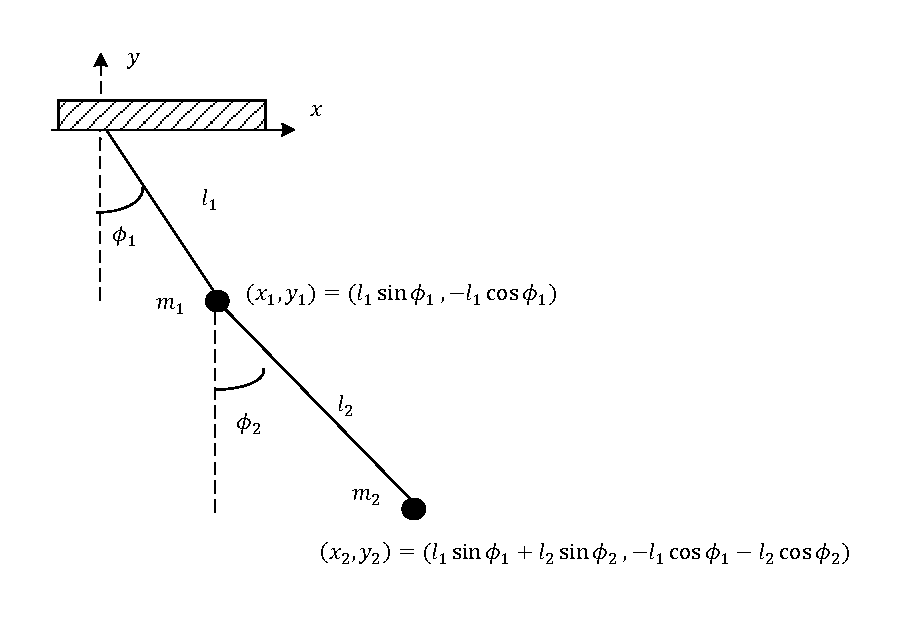
\includegraphics [width=10cm, height=8cm] {DoublePendulum}}
\caption{Pendulu bikoitza.}
\label{fig:41}
\end{figure} 

\subsection{Ekuazioak.}

\paragraph*{\textbf{Hamiltondarra.}}

\begin{equation*}
q=(\Theta_1,\Theta_2) \ \ , \ \ p=(P_1,P_2) \ \ , 
\end{equation*}

\begin{equation*} \label{eq:2}
H(q,p)= \bigg(\frac {C1 \ P_1^2 + C2 \ P_2^2 + 
 C3 \ P_1 \ P_2 \ \cos(\Theta_1 - \Theta_2)} {
 (C4 + C5 \ \sin^2 (Q_1 - Q_2))}\bigg)\\
       -C6 \ \cos(\Theta_1)-\ C7 \ \cos(\Theta_2), 
\end{equation*}

non,
\begin{align*}
C1 &= l_2^2*m_2, & C2 = l_1^2*(m_1 + m_2),\\
C3 &= -2*l_1*l_2*l_2, & C4 = 2*l_1^2*l_2^2*m_2*m_1,\\
C5 &= 2*m_1^2*l_2^2*m_2^2, & C6 = g*l_1*(m_1 + m_2),\\
C7 &= g*l_2*m_2.
\end{align*}

\paragraph*{\textbf{Ekuazio diferentzialak.}}

\begin{align*}
\dot{\Theta_1} & = \frac {2*C1*P1+C3*\cos(Q1-Q2)*P2}{aux1},\\
\dot{\Theta_2} & = \frac{(2*C2*P2+C3*\cos(Q1-Q2)*P1)}{aux1},\\
\dot{P1} &=-(aux4+C6*\sin(Q1)), \\
\dot{P1} &=(aux4-C7*\sin(Q2)).
\end{align*}

non,
\begin{align*}
aux1 &=C4+C5*\sin(Q1-Q2)*\sin(Q1-Q2), \\
aux2 &=C3*\cos(Q1-Q2),\\
aux3 &=2*C5*\sin(Q1-Q2)*\cos(Q1-Q2),
\end{align*}
\begin{multline*}
aux4 =(-1/aux2)*(C1*P1^2+C2*P2^2+P1*P2*aux2*aux3)\\
       -(C3*P1*P2*\sin(Q1-Q2))/{aux1}. 
\end{multline*}

\subsection{Hasierako balioak.}

\paragraph*{\textbf{Sistemaren parametroak}.} 
Gure esperimentuetarako honako parametroak kontsideratuko ditugu,
\begin{align*} 
\label{eq:17}
g & =9.8 \ m/sec^2,\\
l_1 & =1 \ m \ , \ l_2=1 \ m\ ,\\
m_1 & =1 \ kg\ , \ m_2=1 \ kg.
\end{align*} 

\paragraph*{\textbf{Hasierako balioak}.}
Pendulu bikoitza izaera kaotikoa duen sistema ez-lineala da. Zentzu honetan bi hasierako balio ezberdin kontsideratu ditugu \cite{Papadrakakis}:

\begin{enumerate}
   \item Hasierako balio ez-kaotikoak: 
     
   \ $q(0)=(1.1, \ 0)$ \ , \ $p(0)=(0,\ 2.7746)$.    
   \item Hasierako balio kaotikoak: 
      
   $q(0)=(0, \ 0)$ \ , \ \ \  $p(0)=(0,\ 3.873)$.
\end{enumerate}


\subsection{Kodeak.}

Mathematican DoublePendulum.m paketean honako funtzioak inplementatu ditugu:

\begin{enumerate}
   \item Hamiltondarra: DoublePendulumHam.
   \item EDA: DoublePendulumODE.
   \item Jakobiarra: DoublePendulumJAC.
\end{enumerate}

\paragraph*{}C-lengoaian GaussUserProblem.c fitxategian honako funtzioak inplementatu ditugu:

\begin{enumerate}
   \item Hamiltondarra: HamPendulum().
   \item EDA: OdePendulum().
   \item Jakobiarra: JacPendulum().
\end{enumerate}

\section{N-Body problema.}

N-gorputzeko problema grabitazionalari dagokionez, Eguzki sistemaren eredu sinplea integratuko dugu. Eguzki-sistemaren gorputzak masa puntualak kontsideratuko ditugu eta gure ekuazio diferentzialek, soilik gorputz hauen arteko erakarpen grabitazionalak kontutan hartu ditugu. Beraz, eguzki-sistemaren eredu konplexuagoetako erlatibitate efektua, gorputzen formaren eragina, eta beste zenbait indar ez-grabitazionalak ez dira kontutan hartu.

$(N+1)$ gorputz kopurua izanik, $\mathbf{q_i},\mathbf{p_i}\in \mathbb{R}^3$, $m_i \in \mathbb{R}, \ \ i=0,\dots,N$ gorputz bakoitzaren kokapena, momentua eta masa dira. Bestalde , momentua era honetan definituko dugu $\mathbf{p_i}=m_i*\mathbf{v_i}$ non $\dot{\mathbf{q_i}}=\mathbf{v_i}$ den.

\subsection{Zailtasunak.}

Kontutan hartzekoa da eguzki-sistemaren integrazioaren urrats kopuru handia. Eguzki-sistemaren bizi iraupena $5  \times 10^9$ urtetakoa izanik eta integrazioetako ohiko urratsa  $h=0.0025$ urteko bada (orbita txikieneko periodoaren $ \%1$ ), eman beharreko urrats kopurua $2 \times 10^{12}$ izango da. Era berean, kanpo planeten integrazioa $5 \times 10^{10}$ urrats kopuru ingurukoa da.     

Eguzki-sistemaren gorputzen denbora eskala oso ezberdinak dira. Gainera ilargia kontsideratuko bagenu, lurrarekiko distantzia $D_M=3.844 \times 10^8$ eta periodoa $P_M=27.32$ egunekoa. 

\begin{table} [h!]
\caption{}
\label{tab:1}       % Give a unique label
\begin{tabular}{c c c} 
\hline
 Planeta   &  Axis a        & Periodoa    \\   
           &   AU          &   years      \\ \hline
 Merkurio  &   $0.39$      &  $0.24$     \\
 Venus     &   $0.72$      &  $0.007$    \\
 Earth     &   $1.00$      &  $1.007$    \\
 Mars      &   $1.52$      &  $1.88$     \\ \hline
 Jupiter   &   $5.20$      &  $11.86$    \\
 Saturn    &   $9.54$      &  $29.42$    \\
 Uranus    &   $19.19$     &  $83.75$    \\
 Neptune   &   $30.06$     &  $163.72$    \\
 Pluto     &   $39.53$     &  $248.02$    \\
\hline
\end{tabular}
\end{table}

\begin{figure}[h]
\centering
\subfloat[Eguzki-sistema.]{
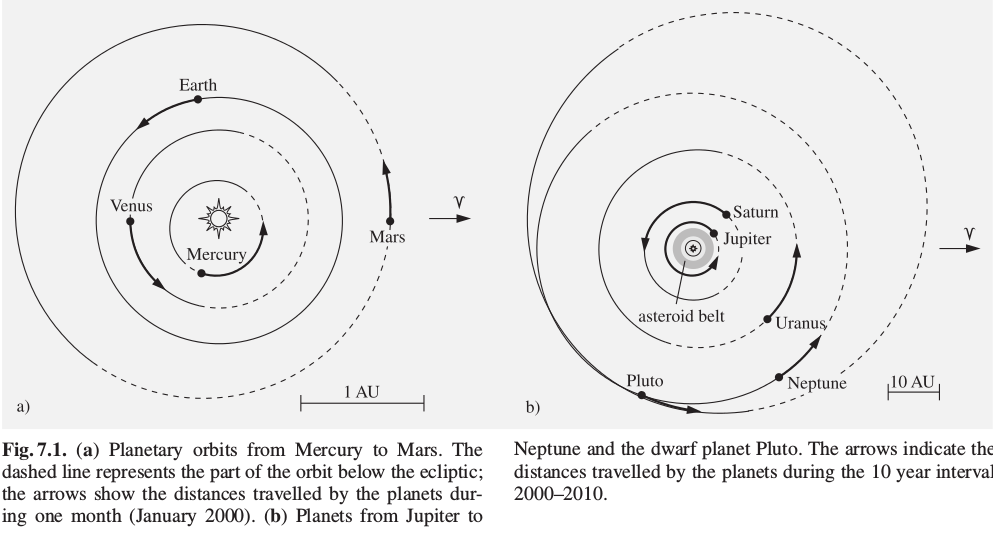
\includegraphics[width=.800\textwidth]{eguzkisistema3}
}
\caption{ \small Eguzki-sistema.}
\label{fig:eguzki-sistema}
\end{figure}


\subsection{Ekuazio barizentrikoak.}

\paragraph*{Hamiltondarra.}

\begin{equation}
H(q,p)=\frac{1}{2}\ \sum^N_{i=0}{\ \frac{{\|p_i\|}^2}{m_i}}-G\ \sum^N_{0\le i<j\le N}{\frac{m_im_j}{\|q_i-q_j\|}} 
\end{equation}

\paragraph*{Ekuazio diferentzialak.}

\begin{equation}
\dot{q_i}=v_i, \ \  i=0,1,\dots, N
\end{equation}

\begin{equation}
\dot{v_i}= \sum_{j=0,j \neq i}^{N} \frac{Gm_j}{\|q_j-q_i\|^3} (q_j-q_i) , \ \  i=0,1,\dots, N
\end{equation}

\paragraph*{Ekuazio diferentzialak.}
Eguzkiaren erlatibitate efektua kontutan hartzen duten ekuazio diferentzialak azalduko ditugu.

\begin{equation}
\dot{q_i}=v_i, \  i=0,1,\dots N
\end{equation}

\begin{multline} 
\dot{v_i}= \sum_{j=0,j \neq i}^{N} \frac{Gm_j}{\|q_j-q_i\|^3} (q_j-q_i)
           \bigg(1- \frac{2(\beta+\gamma)}{c^2} \sum\limits_{k=0, k \neq i}^{N} \frac{Gm_k}{\|q_k-q_i\|} 
                  - \frac{2\beta-1}{c^2}        \sum\limits_{k=0, k \neq j}^{N} \frac{Gm_k}{\|q_k-q_j\|} \\
                  + \gamma \big(\frac{v_i}{c}\big)^2 + (1+\gamma) \big(\frac{v_j}{c} \big)^2 
                  - \frac{2(1+\gamma)}{c^2} v_i \ v_j \\
                  - \frac{3}{2c^2} \big(\frac{(q_i-q_j) v_j}{\|q_j-q_i\|} \big)^2+                  
                  \frac{1}{2c^2}(q_j-q_i) \dot{v_i} \bigg) \\
           + \frac{1}{c^2} \sum_{j=0,j \neq i}^{N} \frac{Gm_j}{\|q_j-q_i\|^3} 
             ((q_i-q_l) ((2+2\gamma)v_i-(1+2\gamma)v_j)) (v_i-v_j) \\
           + \frac{3+4\gamma}{2c^2} \sum_{j=0,j \neq i}^{N} \frac{Gm_j \dot{v_j}}{\|q_j-q_i\|}                                      
\end{multline}

\begin{table}[h]
\caption{Konstanteak}
\label{tab:1}       % Give a unique label
\centering
\begin{tabular}{ c c c }
\hline
  c             &  $299792.458$ km/s           & Argiaren abiadura  \\
\hline
  au            &  $149597870.700$ km           & Astronomical unit  \\
\hline 	       
$\beta$          & $1.0$                       & PPN parametroa     \\
\hline 
$\gamma$         & $1.0$                       & PPN parametroa     \\
\hline
\end{tabular}
\end{table}


\subsection{Ekuazio Heliozentrikoak.}

Ohikoa da ekuazio diferentzialak koordenatu heliozentrikoen (eguzkiaren zentroarekiko) arabera definitzea. Argitu koordenatu heliozentrikoak ere modu ezberdinean eman daitezkeela eta guk koordenatu \emph{heliozentriko kanonikoak} deiturikoak erabili ditugula.

\begin{align*}
\dot{\mathbf{Q_i}} &=\mathbf{V_i}+ \sum\limits_{j\ne i,\ j=1}^{N} \frac{\mathbf{V_j} \ m_j}{(m_0+m_j)},\\
\dot{\mathbf{V_i}} &=- G  \ \frac{(m_0+m_i)}{\|\mathbf{Q_i}\|^3 }\ \mathbf{Q_i}-G \ \frac{(m_0+m_i)}{m_0}
                    \sum\limits_{j \ne i , \ j=1}^{N} \bigg( \frac{m_j}{\|\mathbf{Q_i}-\mathbf{Q_j}\|^3} (\mathbf{Q_i-\mathbf{Q_j}})     \bigg), \ \ i=1,\dots, N.
\end{align*}

Ekuazioen garapen osoa eranskinean eman dugu.

\subsection{Hasierako balioak.}

Eguzki eta planeten hasierako kokapenak (au) eta abiadurak (au/day), Julian data (TDB) $2440400.5$ ($1969$. ekainaren $28$) eta ICRFR2 (International Celestial Reference Frame) koordenatu sisteman \cite{Folkner2014},

\begin{table}[h]
\caption[Eguzki-sistemaren hasierako balioak]{Eguzki eta planeten hasierako balioak integrazio jatorriarekiko.}
\label{tab:1}       % Give a unique label
\centering
\resizebox{\textwidth}{!}{%
\begin{tabular}{ c c c c c }
\hline 
  Eguzkia        &  $x,y,z$         & $0.00450250878464055477$ & $0.00076707642709100705$ &	$0.00026605791776697764$    \\\hline
                 &  $v_x,v_y,v_z$   & $-0.00000035174953607552$ & $0.00000517762640983341$ & $0.00000222910217891203$    \\\hline
  Mercury        &  $x,y,z$         &  $0.36176271656028195477$ & $-0.09078197215676599295$ &	$-0.08571497256275117236$ \\\hline
                 &  $v_x,v_y,v_z$   &  $0.00336749397200575848$ & $0.02489452055768343341$ &	$0.01294630040970409203$ \\\hline
  Venus          &  $x,y,z$         &  $0.61275194083507215477$ & $-0.34836536903362219295$	& $-0.19527828667594382236$ \\\hline
                 &  $v_x,v_y,v_z$   &  $0.01095206842352823448$ & $0.01561768426786768341$ &	$0.00633110570297786403$\\\hline  
  EMB            &  $x,y,z$         &  $0.12051741410138465477$ & $-0.92583847476914859295$ &	$-0.40154022645315222236$\\\hline
                 &  $v_x,v_y,v_z$   &  $0.01681126830978379448$ & $0.00174830923073434441$ &	$0.00075820289738312913$\\\hline 
  Mars           &  $x,y,z$         & $-0.11018607714879824523$ & $-1.32759945030298299295$ &	$-0.60588914048429142236$ \\\hline
                 &  $v_x,v_y,v_z$   &  $0.01448165305704756448$ & $0.00024246307683646861$ & $-0.00028152072792433877$   \\\hline 
  Jupiter        &  $x,y,z$         &  $-5.37970676855393644523$ & $-0.83048132656339789295$ & $-0.22482887442656542236$ \\\hline
                 &  $v_x,v_y,v_z$   & $0.00109201259423733748$ & $-0.00651811661280738459$ &	$-0.00282078276229867897$\\\hline                     
  Saturn         &  $x,y,z$         &  $7.89439068290953155477$ & $4.59647805517127300705$ &	$1.55869584283189997764$	    \\\hline
                 &  $v_x,v_y,v_z$   &  $-0.00321755651650091552$ & $0.00433581034174662541$ & $0.00192864631686015503$     \\\hline
  Uranus         &  $x,y,z$         &  $-18.26540225387235944523$ &	$-1.16195541867586999295$ &	 $-0.25010605772133802236$\\\hline
                 &  $v_x,v_y,v_z$   &  $0.00022119039101561468$ & $-0.00376247500810884459$ &	$-0.00165101502742994997$ \\\hline
  Neptune        &  $x,y,z$         &  $-16.05503578023336944523$ &	$-23.94219155985470899295$ &	 $-9.40015796880239402236$    \\\hline
                 &  $v_x,v_y,v_z$   & $0.00264276984798005548$ & $-0.00149831255054097759$ &	$-0.00067904196080291327$     \\\hline
  Pluto          &  $x,y,z$         &  $-30.48331376718383944523$ & $-0.87240555684104999295$ &	 $8.91157617249954997764$ \\\hline
                 &  $v_x,v_y,v_z$   &  $0.00032220737349778078$ & $-0.00314357639364532859$ &	$-0.00107794975959731297$\\\hline       
\end{tabular}}
\end{table}

\begin{table}[h]
\caption{Ilargiaren Lurrarekiko hasierako balioak.}
\label{tab:1}       % Give a unique label
\centering
\resizebox{\textwidth}{!}{%
\begin{tabular}{ c c c c c }
\hline 
  Ilargia         &  $x,y,z$         & $-0.00080817735147818490$ &	$-0.00199462998549701300$ &	$-0.00108726268307068900$    \\\hline
                 &  $v_x,v_y,v_z$   & $0.00060108481561422370$ & $-0.00016744546915764980$ &	$-0.00008556214140094871$ \\\hline
\end{tabular}}
\end{table}
                 
\begin{table}[h]
\caption{Planeten masa parametroak.}
\label{tab:1}       % Give a unique label
\centering
\begin{tabular}{ c c }
\hline 
  Gorputza         &  GM ($au^3/day^3$)          \\\hline
  Eguzkia          &  $0.295912208285591100E-03$ \\\hline
  Mercury          &  $0.491248045036476000E-10$ \\\hline   
  Venus            &  $0.724345233264412000E-09$ \\\hline
  Earth            &  $0.888769244512563400E-09$ \\\hline
  Mars             &  $0.954954869555077000E-10$ \\\hline
  Jupiter          &  $0.282534584083387000E-06$ \\\hline
  Saturn           &  $0.845970607324503000E-07$ \\\hline
  Uranus           &  $0.129202482578296000E-07$ \\\hline
  Neptune          &  $0.152435734788511000E-07$ \\\hline
  Pluto            &  $0.217844105197418000E-11$ \\\hline
  Moon             &  $0.109318945074237400E-10$ \\\hline
\end{tabular}
\end{table}


\paragraph*{Masa zentrua.} Integrazio hasieran, gorputzen kokapen eta abiadurak   masa zentruaren kokapen eta abiadurak zero izateko aldatzen dira.

\begin{equation*}
M=\sum\limits_{i=0}^{N}Gm_i
\end{equation*} 

Masa zentruaren kokapena ($Q$) eta abiadura ($V$),
\begin{equation*}
Q=\frac{(\sum\limits_{i=0}^{N} Gm_i*q_i)}{M}, \ V=\frac{(\sum\limits_{i=0}^{N} Gm_i*v_i)}{M}
\end{equation*}

Eta integrazio hasierako balioak,
\begin{equation*}
qnew_i=q_i-R, \ \  vnew_i=v_i-V, \ \ i=0,\dots,N.
\end{equation*}


                 
\subsection{Kodeak.}

\paragraph*{} Mathematicako NBodyProblem.m paketean honako funtzioak garatu ditugu.

\begin{enumerate}
   \item Hamiltondarra: NBodyHAM.
   \item EDA: NBodyODE.
   \item Jakobiarra: Ez dut garatu.
\end{enumerate}

-\paragraph*{} C-lengoaiako inplementazioa:

\begin{enumerate}
   \item Hamiltondarra: HamNBody().
   \item EDA: OdeNbody().
   \item Jakobiarra: JacNBody().
\end{enumerate}

\section{Laburpena.}

\chapter{Koma higikorreko aritmetika}
\label{sec:4}

\section{Sarrera}

Konputagailuetan, zenbaki errealak ($\mathbb{R}$) bit kopuru finituaren bidez adierazi behar dira eta honetarako, koma-higikorreko adierazpen sistema ($\mathbb{F}\subset \mathbb{R}$) erabiltzen da. Zenbaki erreal batzuk, $\mathbb{F}$ sisteman adierazpen zehatza dute, baina beste batzuk hurbildu egin behar dira.  Era berean, eragiketa aritmetikoen ($+,-,*,/$) kalkulu gehienetan ere emaitzaren hurbilpena egin beha da. $\mathbb{R}$ sistematik $\mathbb{F}$ sistemara bihurtzeko funtzioari biribiltzea esaten zaio. Oro har, konputazio zientzian biribiltze errore honen eragina garrantzitsua da eta errorea gutxitzeko ahalegin berezia beharrezkoa da.

Egungo konputagailuen koma-higikorreko aritmetikaren inplementazioak, \emph{IEEE-$754$} estandarrean \cite{IEEE2008} oinarritzen dira. 
\emph{IEEE-$754$} estandarrak, koma-higikorreko aritmetikaren konputaziorako formatu eta metodoak definitzen ditu. Konputazioen fidagarritasuna eta aplikazioen portabilitatea bermatzen ditu.    
 
Atal honetan, koma-higikorreko aritmetika eta biribiltze errorearen oinarria azalduko ditugu. Ondoren, konputazioetan biribiltze erroreak gutxitzeko teknika ezagun batzuk azalduko ditugu. 

\section{\emph{IEEE-754} estandarra}

Koma-higikorreko zenbaki multzoa finitua da eta ${\mathbb{F}}$ izendatuko dugu. Koma-higikorreko adierazpen zehatza duten zenbaki errealei koma-higikorreko zenbakiak deritzogu, 
\begin{equation*}
\mathbb{F}\subset \mathbb{R}.
\end{equation*}

$\mathbb{F}$ zenbaki multzoa, \ref{fig:FloatNumberLine}irudian laburtu dugu. Bai zenbaki positiboentzat, bai negatiboentzat, adieraz daitekeen zenbaki handienaren eta txikienaren arteko balio bakanez osatuta dago. Multzoaren kanpoaldean zenbaki hauek guztiak ditugu: batetik overflow tartean $(-\infty,\max_{x \in \mathbb{F_{-}}}|x|)$  eta $(\max_{x \in \mathbb{F_{+}}}|x|,\infty+)$ daudenak; bestetik underflow tartean  $(\min_{x \in \mathbb{F_{-}}}|x|,0)$ eta $(0,\min_{x \in \mathbb{F_{+}}}|x|)$ daudenak. 

\begin{figure}[h]
\centerline{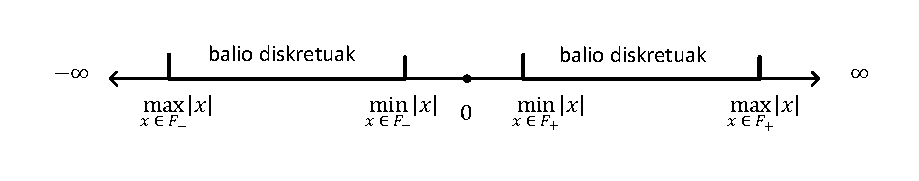
\includegraphics[width=14cm, height=3cm] {ZenbakiErrealak}}
\caption[Koma-higikorreko zenbakien multzoa]{Koma-higikorreko zenbakien multzoa}
\label{fig:FloatNumberLine}
\end{figure} 

IEEE-754 estandarraren arabera, $n$-biteko koma-higikorreko adierazpenak bi zati ditu (ikus \ref{fig:32bitKomaHigikorra} irudiko adibidea),
\begin{enumerate}
\item $m$ bitez osatutako zatia, mantisa ($M$) izenekoa. Horietako bit batek ($S$) zeinua adierazten du. Bestalde $M$ mantisa modu normalizatu honetan emana da, $\pm 1.F$ eta zati erreala ($F$) bakarrik gorde behar da.   
\item Esponentea ($E$), $(n-m)$ bitez adierazitako zenbaki osoa. Zeinuarentzat ez da bit zehatzik, baizik \emph{bias} izeneko balio bat kenduz adierazten dira zenbaki positiboak eta negatiboak.  
\end{enumerate}

Beraz, oinarri bitarrean koma-higikorreko zenbaki hauek adierazten dira,
\begin{equation*}
M \times b^E, \ b=2,
\end{equation*}
eta biribiltze unitatea (\emph{unit roundoff}) era honetan definituko dugu,
\begin{equation*}
u=2^{-m}.
\end{equation*} 

\begin{figure}[h]
\centerline{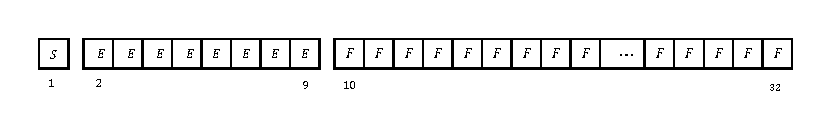
\includegraphics[width=12cm, height=2cm] {ZenbakiErrealak2}}
\caption[32-biteko koma-higikorra]{\small $32$-biteko koma-higikorreko zenbakiaren adierazpena: esponentearentzat  8-bit eta mantisarentzat  $24$-bit (bit bat zeinuarentzat eta beste $23$ bit, $1.F$ eran normalizatutako mantisarentzat) banatuta}
\label{fig:32bitKomaHigikorra}
\end{figure} 

IEEE-$754$ estandarrean, oinarri bitarreko koma-higikorreko hiru formatu definitzen dira: bata doitasun arrunta (\emph{single precision}), bestea doitasun bikoitza (\emph{double precision}) eta hirugarrena doitasun laukoitza (\emph{quadruple precision}) izenekoak (\ref{tab:koma-higikorreko-aritmetikak} Taula).

\begin{table} [h!]
\caption[IEEE-754 koma-higikorreko formatuak]{IEEE-754 koma-higikorreko formatuak}
\label{tab:koma-higikorreko-aritmetikak}       % Give a unique label
\centering
\begin{tabular}{ l c c c l c} 
 \hline
 Formatoa      &  Tamaina    & Mantisa   & Esponentea  & Tartea           &  $u=2^{-m}$          \\
               &    n        & m         & n-m         &                  &                      \\
   \hline
% Half     & 16 bit      & 11  & 5  & $2^{\pm 16}$     &  $5 \times 10^{-4}$   \\ 
 Arrunta   & 32 bit      & 24  & 8  & $10^{\pm 38}$    &  $6 \times 10^{-8}$   \\	    
 Bikoitza  & 64 bit      & 53  & 11 & $10^{\pm 308}$   &  $1 \times 10^{-16}$   \\
 Laukoitza & 128 bit     & 113 & 15 & $10^{\pm 11356}$ &  $1 \times 10^{-35}$   \\
\hline
\end{tabular}
\end{table}


Doitasun bikoitzeko oinarrizko eragiketak (batuketa, kenketa, biderketa, zatiketa, eta erro karratua) hardware bidez exekutatzen dira \cite{Muller2009} eta azkarrak dira. Makina ziklo bakoitzeko, $2$ eta $4$ batuketa, kenketa edo biderketa egin ohi dira; zatiketa eta erro karratua aldiz, eragiketa motelagoak dira. Bestalde, doitasun arruntaren  aritmetika, doitasun bikoitza baino azkarragoa da: garraiatu behar den bit kopuru erdia delako eta gainera, hardware bereziei esker (adibidez \emph{Intel} makinetan \emph{SSE} moduluak), eragiketa aritmetikoak azkarragoak direlako. 2008. urtean, IEEE-$754$ estandarrak, $128$-biteko koma-higikorreko aritmetika onartu zuen, baina  inplementazioa  softwarez bidezkoa da eta exekuzioa, gutxi gorabehera, doitasun bikoitzeko aritmetika baino 10-15 aldiz motelagoa da.

Problema batzuk, doitasun bikoitza baino doitasun handiagoa behar dute \cite{Joldes2016}. Doitasun laukoitza edo altuagoa, software liburutegien bidez emulatu ohi dira. Doitasun altuko zenbakiak adierazteko nagusiki bi modu bereizten dira:   

\begin{enumerate}
\item \emph{Digitu-anitzeko adierazpena}. Zenbakiak esponente bakarra eta mantisa bat baino gehiagorekin adierazten dira (adb. \emph{GNU MPFR liburutegia} \cite{Fousse2007}).
\item \emph{Termino-anitzeko adierazpena}. Zenbakiak  ebaluatu gabeko hainbat koma-higikorreko makina zenbaki estandarren batura gisa adierazten dira (adb. Bailey QD liburutegia) \cite{Hida2001} eta exekuzioaren ikuspegitik, hardware bidezko inplementazioaren abantaila dute.    
\end{enumerate}

Doitasun laukoitzeko gure esperimentuetarako, \emph{GCC libquadmath} liburutegia \cite{libquad} erabili dugu. Doitasun laukoitzean exekutatutako integrazioen zenbakizko soluzioak, soluzio zehatzak kontsideratu ditugu eta  doitasun bikoitzeko inplementazioaren errorea, soluzio zehatzarekiko diferentzia gisa kalkulatu dugu. 

Laskar-ek epe luzeko eguzki-sistemaren simulazioaren ($-250$ eta $+250$ milioitako integrazio tartea) konputaziorako kalkuluak \cite{Laskar2011}, kontu handiz eta doitasun handian egin behar ditu. Dena den, era honetako problemak salbuespenak dira eta ez da ohikoa izaten doitasun handian lan egin beharra. Egia da ere, neurri fisiko oso gutxi ezagutzen direla  hain doitasun handian (adibidez $50$-bitekin, Lurra eta Ilargiaren arteko distantzia, milimetroko errorearekin adieraz daiteke).  


\section{Biribiltze errorea}

Zenbakizko integrazioen errorea, trunkatze eta biribiltze errorez osatuta dago. Urrats luzera nahi bezain txikia aukeratuz, trunkatze errorea biribiltze errorea baino txikiago izango da eta beraz, zenbakizko integrazio hauetan errorean biribiltze errorea nagusitzen da. Epe luzeko eta doitasun handiko integrazioetan, urrats luzera txikia erabiltzen denez, biribiltze errorea gutxitzea funtsezkoa izango da.     

Bi biribiltze errore mota bereiziko ditugu, bata adierazpenaren errorea eta bestea, aritmetikaren errorea.  

\subsection*{Adierazpenaren errorea} 

Zenbaki erreal batzuk, $\mathbb{F}$ koma-higikorreko multzoan zehazki adieraz daitezke eta beste batzuk ordea, hurbilpen batez adierazi behar dira. $x \in \mathbb{R}$ izanik, $fl: \mathbb{R} \rightarrow \mathbb{F}$ koma-higikorreko zenbakia esleitzen dion funtzioari deituko diogu:  $x \in \mathbb{R}$ balioaren gertuen dagoen  $fl(x) \in \mathbb{F}$ itzultzen duen funtzioa bezala definitzen da. Hau da, $f_1,f_2 \in \mathbb{F}$ jarraian dauden koma-higikorreko zenbakiak  badira eta $x \in \mathbb{R}, \ f_1\leqslant x \leqslant f_2$ bada,
\begin{equation*}
fl(x)=
\left\{
        \begin{array}{lc}
        f_1 & \mathrm{if} \ |x-f_1| < |x-f_2| \\
        f_2 & \mathrm{if} \ |x-f_1| \geqslant |x-f_2| 
        \end{array}.
\right.
\end{equation*}  

Jarraian, koma-higikorreko adierazpenaren errore absolutua eta errore erlatiboa finkatuko ditugu.
\begin{itemize}
\item Errore absolutua,
\begin{equation*}
\triangle x= fl(x)-x= \tilde{x}-x. 
\end{equation*} 
\item Errore erlatiboa, 
\begin{equation*}
\delta x =\frac{\triangle x}{x} = \frac{\tilde{x}-x}{x}. 
\end{equation*}
\item Aurreko bi definizioen ondorioz honako formula erabilgarria dugu,
\begin{equation*}
\tilde{x}= x+\triangle x = x \ (1+\delta x).
\end{equation*}
\end{itemize}

Koma-higikorreko zenbaki sistema bitarrean ($m=$ mantisa adierazteko bit kopurua izanik) $|x|$ balioa, $\mathbb{F}$ multzoaren zenbaki txikienaren eta handienaren artean badago,
\begin{equation*}
 |\delta x|< u \ \ \text{non} \ \ u=2^{-m},
 \end{equation*}
bermatuta dagoela froga daiteke \cite{Corless2013}.

\subsection*{Aritmetikaren errorea} 

Koma-higikorreko zenbakien arteko eragiketa baten emaitzak, ez du zertan $\mathbb{F}$ multzoan adierazpen zehatza izan  eta orduan, emaitza biribildu egingo  da. Adibidez, $m$ digituzko bi zenbakien biderketaren emaitza zehatza adierazteko, $2m$ digituzko mantisa behar dugu ($m$ digituzko galera) \cite{Fukushima2001}. Salbuespena, biderkagaietako bat $2$-ren berretura denean gertatzen da, orduan biderketa zehatza baita.

\paragraph*{Adibidea.} Demagun lau digitu hamartar errealeko aritmetikarekin ari garela lanean.

Emaitza zehatza, $1,343 \times 2,103 = 2,824229$. 

Hiru digitu hamartar errealeko aritmetika, $1,343 \times 2,103 \approx 2.824$.

\paragraph*{} Hauek zenbaki errealen arteko funtsezko eragiketak badira,  $\ast: \mathbb{R}^2\rightarrow \mathbb{R}$, 
\begin{equation*}
\ast\in \{+,-,\times,/ \},
\end{equation*}
koma-higikorreko zenbakien arteko funtsezko eragiketak era honetan izendatuko ditugu  $\circledast: \mathbb{F}^2\rightarrow \mathbb{F}$,
\begin{equation*}
\circledast\in \{\oplus,\ominus,\otimes,\oslash \}.
\end{equation*}

$\tilde x,\tilde y \in \mathbb{F}$ emanik eta $z= \tilde x \ast \tilde y$ emaitza zehatza bada, $\tilde z= \tilde x \circledast \tilde y$ (edo $\tilde z= fl(\tilde x \ast \tilde y$)) eragiketaren emaitzaren errore absolutua eta errore erlatiboa definituko ditugu,

\begin{itemize}
\item Errore absolutua,
\begin{equation*}
\triangle z=\tilde z-z =(\tilde x \circledast \tilde y) -(\tilde x \ast \tilde y).
\end{equation*} 
\item Errore erlatiboa,
\begin{equation*}
\delta z=\frac{\triangle z}{z}==\frac{(\tilde x \circledast \tilde y) -(\tilde x \ast \tilde y)}{(\tilde x \ast \tilde y)}.
\end{equation*} 
\item Honako erlazio hau ondorioztatu daiteke,
\begin{equation*}
\tilde z=(\tilde x \circledast \tilde y)=z+\triangle z=z \ (1+\delta z).  
\end{equation*}
\end{itemize}

Koma-higikorreko aritmetikan, \ $|\delta z|<u$ \ , non  $u=2^{-m}$, beteko dela froga daiteke \cite{Corless2013}.

\paragraph*{} Zenbakizko algoritmoen biribiltze errorearen eraginaren azterketa formalak, propietate hauetan oinarritzen dira. Bestalde, errore erlatiboak emaitzaren digitu zuzenen kopurua neurtzen du:
\begin{equation*}
\delta z \approx 10^{-k} \Rightarrow \ \approx \ k \ \mbox{digitu hamartar zuzen}.
\end{equation*}  


\subsection*{Biribiltze errorearen hedapena}


Ohiko konputazioetan eragiketa aritmetiko kopuru handia egin behar dugu emaitza lortzeko. Batzuetan, eragiketen biribiltze erroreak elkar ezereztatzen dira baina kasu txarrenean, biribiltze errorea metatu eta magnitude handikoa izan daiteke.   

\paragraph*{Adibidea.} 
Modu honetako batura batean , non $n>2$ eta $\tilde x_1,\dots,\tilde x_n \in \mathbb{F}$,  
\begin{equation*}
\bigoplus_{i=1}^{n}(\tilde x_i)=(\sum\limits_{i=1}^{n} \tilde x_i)(1+\delta),
\end{equation*}
$|\delta|<u \ \text{non} \  u=2^{-m}$ beteko denik, ezin daiteke bermatu. 

\paragraph*{}Analisi zehatza egiten badugu $n=3$ adibiderako, honako espresioa lortzen dugu,
\begin{equation*}
((\tilde x_1 \oplus \tilde x_2) \oplus \tilde x_3)  = 
  \big((\tilde x_1 + \tilde x_2)(1+\delta_1)
  +\tilde x_3 \big) (1+\delta_2), \ \ \delta_1,\delta_2<u.
\end{equation*}

\subsection*{Ezabapen arazoa}

Algoritmoen kalkuluetan, doitasun galera azkarra gerta daiteke. Horren adibidea ezabapen arazoa dugu: oso antzekoak diren bi zenbakiren arteko kendura egiten dugunean gerta daitekeena. 

\paragraph*{Adibidea.} Mathematican kalkulatutako adibide honetan, ezabapen errorea nola gertatzen den erakutsi dugu. 
\begin{lstlisting} [language=Mathematica]
>>  InputForm[N[Pi]]
>> 3.141592653589793

>> y=N[Pi]*10^(-10);
>> InputForm[y]
>> 3.1415926535897934*10^(-10)

>> z=1.+y;
>> InputForm[z]
>> 1.0000000003141594           # 16-digitu hamartar zuzenak.

>> InputForm[z-1.]
>> 3.141593651889707*10^(-10)   # 6-digitu hamartar zuzenak.

\end{lstlisting}


\section{Biribiltze errorea gutxitzeko teknikak}
\label{sec:4.4}

Batuketa eta biderketa eragiketen biribiltze errorea kalkulatzeko algoritmoak ezagunak dira \cite{Dekker1971,Higham2002}. Algoritmo hauek, \emph{termino-gaitzeko adierazpenetan} oinarritzen dira eta baturaren kasuan, batura konpentsatu izeneko algoritmoaren oinarria da. Ikusiko dugun bezala, algoritmo sinpleak dira eta konputazio kostu txikia dute.  

Teknika hauek, zenbakizko integrazioaren inplementazioaren kalkulu "kritikoetan" erabiliko ditugu, soluzioaren doitasuna handitzeko asmoarekin.

\subsection*{Batura: Fast2Sum}

\emph{Fast2Sum} algorithmoa, 1971.ean Dekker-ek  asmatu zuen \cite{Dekker1971}. Koma-higikorreko $\tilde x,\tilde y \in \mathbb{F} \ \text{non} \ |\tilde x| \geq |\tilde y| \ \text{bi zenbakien}$ arteko $\tilde z= \tilde x \oplus \tilde y$ batuketari dagokion $e$ biribiltze errorea  era honetan kalkula daiteke,
%\ \text{non} \ \tilde z+ e=\tilde x+\tilde{y}$ den

\begin{algorithm}[H]
 \BlankLine
 {$\tilde{z}=\tilde{x} \oplus\tilde{y}$\;
  $e=\tilde{y} \ominus (\tilde{z}\ominus\tilde{x})$\;
 }
 \BlankLine
 \caption{Fast2Sum}
 \label{alg:FastSum}
\end{algorithm}

\ref{fig:fast2sum}irudiaren laguntzarekin hobeto uler daiteke batuketaren biribiltze errorearen kalkulua \cite{Higham2002}.

\begin{figure}[h!]
\centerline{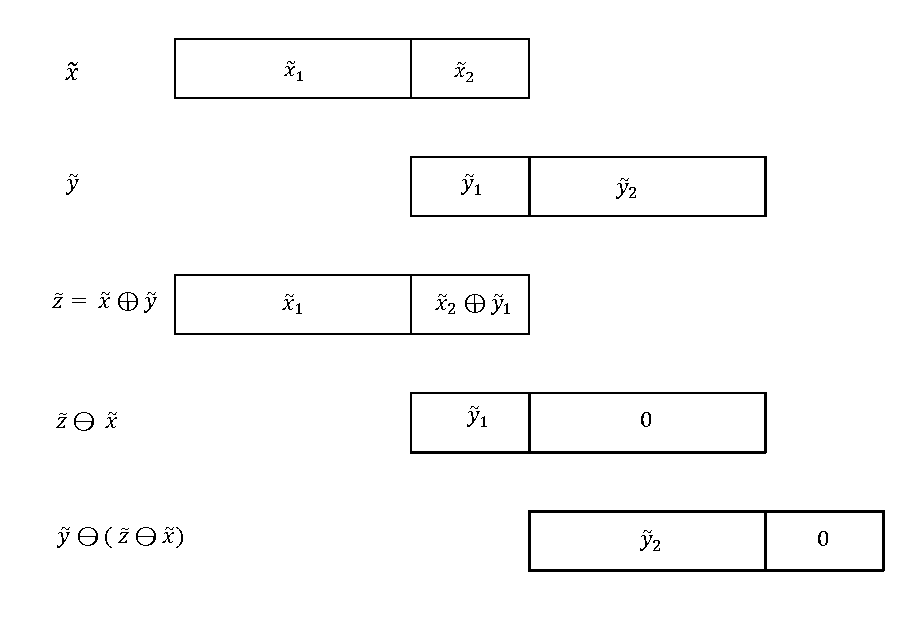
\includegraphics[width=14cm, height=8cm] {Fast2Sum}}
\caption[Batuketaren biribiltze errorea]{Batuketaren biribiltze errorea}
\label{fig:fast2sum}
\end{figure} 

\subsubsection*{Batura konpensatua}

Era honetako batugai askoren arteko batuketan,
\begin{equation*}
z_{n+1}= z_0+\sum\limits_{i=0}^{n} x_i,
\end{equation*}
biribiltze errorea gutxitzeko teknika ezaguna da \cite{Higham2002,Muller2009,Hairer2006}.
Ideia da, bi zenbakien baturan egindako biribiltze errorea lortu, eta errore hau hurrengo baturan erabiltzea. Jarraian azaltzen den moduan, urrats bakoitzaren amaieran $e_{i}$ errore estimazioa  kalkulatuko dugu eta hurrengo urratsean, batugaiari gehituko diogu.

\begin{algorithm}[H]
 \BlankLine
  $\tilde z_0= z_0; \ e_0=0$\;
  \For{$i\leftarrow 0$ \KwTo $n$}
  {
   \BlankLine
    $x=\tilde z_i$\;
    $y= x_i+e_i$\;
    $\tilde z_{i+1}=x+y$\;
    $e_{i+1}=(x-z)+y$\;
   \BlankLine
  }
 \caption{Kahan-en batura konpentsatua}
   \label{alg:KahanBK}
\end{algorithm}

Knuth-ek eta Kahan-ek \cite{Muller2009} frogatu zuten,  batura konpentsatuko algoritmoaren bidez kalkulatutako $z_{n+1}$ baturak honakoa betetzen duela:
\begin{equation*}
\left | z_{n+1} - (z_0+\sum_{i=0}^{n} x_i) \right | \leq (2u+ \mathcal{O}(nu^2)) \left(|z_0|+\sum_{i=1}^{n} |x_0|\right).
\end{equation*}

Jakina da, batugaiak bektoreak diren kasurako, hau da, $\tilde z_0, e_0, x_0, x_1, \dots, x_n \in \mathbb{F}^d$, ~algoritmoa orokor daitekeela. Beraz, \ref{alg:KahanBK} algoritmoa $n$ eta $d$ parametroak dituen funtzio familia gisa interpreta daiteke,
\begin{equation}
\label{eq:batsd}
S_{n,d} : \mathbb{F}^{(n+3)d} \rightarrow \mathbb{F}^{2d},
\end{equation}
zeinek $\tilde z_0, e_0, x_0, x_1, \dots, x_n \in \mathbb{F}^d$ argumentuak emanik, $\tilde z_{n+1}, e_{n+1} \in \mathbb{F}^d$ balioak itzultzen dituen, eta ($\tilde z_{n+1}+e_{n+1}) \approx \tilde (z_0+e_0+x_0+x_1+ \dots+x_n$) hurbilketa den.

\subsubsection*{Zenbakizko integrazioak}
 
Zenbakizko integrazioetan, $n=1,2,\dots$ balioentzat era honetako baturak kalkulatu behar ditugu \cite{Hairer2006},
\begin{equation*}
y_{n+1}=y_n+\delta_n,
\end{equation*}  
non $|\delta_n|<|y_n|$ izan ohi den. Beraz, integrazioaren batura honen birbiltze errorea gutxitzeko batura konpentsatua erabiliko dugu.  

$y_{n+1} \in \mathbb{R}^{d},\quad y_{n+1}=\tilde y_{n}+\tilde \delta_n$ batura zehatza izanik eta $\tilde y_{n+1} \in \mathbb{F}^{d}, \quad \tilde y_{n+1}=\tilde y_{n} \oplus \tilde \delta_n$ koma-higikorreko hurbilpena izanik, batura konpentsatuaren bidez lortutako errorearen estimazioa $e_{n+1}$, \ref{alg:batkp}~algoritmoa jarraituz lor daiteke eta baturan egindako biribiltze errore zehatza da, 
\begin{equation}
y_{n+1}=\tilde {y}_{n+1}+e_{n+1}. 
\end{equation}

\begin{algorithm}[H]
 \BlankLine
  $\tilde{y}_{0}=fl(y_{0}); \ e_0=fl(y_0-\tilde{y}_0)$\;
 \BlankLine
  \For{$n=0,1,2,\dots \quad$}
  {
   \BlankLine
    $inc=\tilde {\delta}_n \oplus e_n$\;
    $\tilde {y}_{n+1}=\tilde{y}_n \oplus inc$\;
    $e_{n+1}=(\tilde{y}_n \ominus \tilde {y}_{n+1}) \oplus inc$\;
   \BlankLine
  }
 \caption{Batura konpentsatua (zenbakizko integrazioa)}
 \label{alg:batkp}
\end{algorithm}


Goian aipatutako ideia,  beste ikuspegi batetik ere uler daiteke. Zenbakizko soluzioa, doitasun bikoitzeko bi balioen batura gisa $y_n=\tilde{y}_n+e_n$ (ia doitasun laukoitza), adierazten ari gara  eta beraz, interpretazio honen arabera, konputazio eragiketa batzuk ia doitasun laukoitzean egiten ariko ginateke. Zentzu honetan gure inplementazioan, hasierako balio zehatza $y_0=y(t_0)$, bi balioen batura gisa $y_0=\tilde{y}_0+e_0$ ulertu behar da eta era honetan hasieratuko dugu,
\begin{align*}
\tilde{y}_0 &=fl(y_0) ,\\
e_0 &=fl(y_0-\tilde{y}_0).
\end{align*}

\subsection*{Bidekerta: 2MultFMA}

\emph{IEEE 754-2008} estandarrean, \emph{FMA} \cite{Muller2009} (\emph{fused multiply-add}) instrukzioa gehitu zen eta hurrengo urteetan, ordenagailu arruntetan zabaltzea espero da. Instrukzio honen garrantzia handia da: orokorrean konputazioak azkartzen ditu eta biderketa eskalarren, matrize biderkaduren eta polinomio ebaluazioen biribiltze errorea txikitzen du. \emph{FMA} instrukzioa, zatiketa eta erro karratuaren algoritmo azkarren diseinuan ere erabiltzen da.

\emph{FMA} instrukzioak, era honetako konputazioetan biribiltze errore bakarra bermatzen du,
\begin{equation*}
fl(\tilde x \times \tilde y \pm \tilde z)= (\tilde x \times \tilde y\pm \tilde z) (1+\delta), \ \delta<u \ \ \text{non} \ \ u=2^{-m}.
\end{equation*}
 

\emph{FMA}  instrukzioa erabilgarri dagoenean, biderketaren biribiltze errorea kalkulatzea erraza da; $\tilde x,\tilde y \in \mathbb{F}$ bi zenbakien arteko biderketari $\tilde z= fl(\tilde x \times \tilde y)$ dagokion biribiltze errorea $e, \ \text{non} \  \tilde{z}+ e=\tilde x \times \tilde y$ den, era honetan kalkulatu daiteke,

\begin{algorithm}[H]
 \BlankLine
 {$\tilde{z}=fl(\tilde{x}\times\tilde{y})$\;
  $e=fl(\tilde{x}\times\tilde{y}- \tilde{z})$\;
 }
 \BlankLine
 \caption{2MultFMA}
 \label{alg:2MultFMA}
\end{algorithm}

\subsection*{Sterbenz Teorema}
Sterbenz teoremaren arabera \cite{Sterbenz1973}, bi zenbaki elkarrekiko  gertu daudenean, honako baldintza betetzen bada, horien arteko kendura zehatza da.
\begin{equation}
\label{eq:4311}
x,y \in \mathbb{F}, \ \ \frac{y}{2}\leq x \leq 2y \ \ \ \Rightarrow \ \ \ x-y\in \mathbb{F}.
\end{equation}


\section{Laburpena}

Atal honetan, koma-higikorreko aritmetikaren deskribapena egin ondoren, konputazioen doitasuna handitzeko tresnak azaldu ditugu. Tresna hauek, konputazio kostu txikia dute eta zenbakizko integrazioetan, biribiltze errorea txikitzeko aplikatuko ditugu.  

Koma-higikorreko aritmetikan sakontzeko honako bibliografia azpimarratuko dugu: \cite{Overton2001,Muller2009,Higham2002,Corless2013}.


\chapter{Zientzia konputazioa.}

\epigraph{Processor speed doubles every 18 months.}{\textit {Moore's Law (1965)}}
\epigraph{Number of cores per chip can double every two years.}{\textit Moore's Law Reinterpreter (2006)}

\section{Sarrera.}

Gaur-egungo konputagailuak (super-konputagailu, eramangarri,...) orokorrean paraleloak dira. 1986-2002 urteen artean, txip barruan transistore dentsitatea handitzen zen heinean, prozesadore bakarreko konputagailuen eraginkortasuna hobetuz joan zen. Baina teknologi-garapena muga fisikoetara iritsita, bide honetatik konputagailuen abiadura hobetzea ezinezkoa bilakatu zen (Irudia \ref{fig:51}). Horrela, 2005.urtetik aurrera fabrikatzaileek konputagailuen gaitasuna hobetzeko, txipan prozesadore bat baino gehiago erabiltzea erabaki zuten.      

\begin{figure}[h]
\centerline{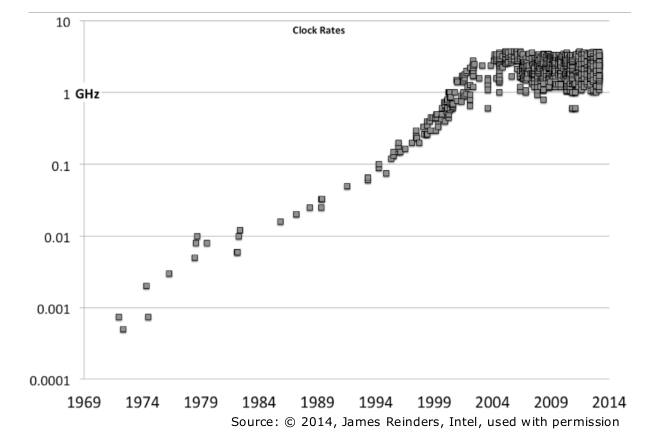
\includegraphics[width=10cm, height=6cm] {ProcessorClock}}
\caption[Processor clock rate.]{\small Processor clock rate growth halted around 2005.}
\label{fig:51}
\end{figure} 

%\begin{figure}[h]
%\centerline{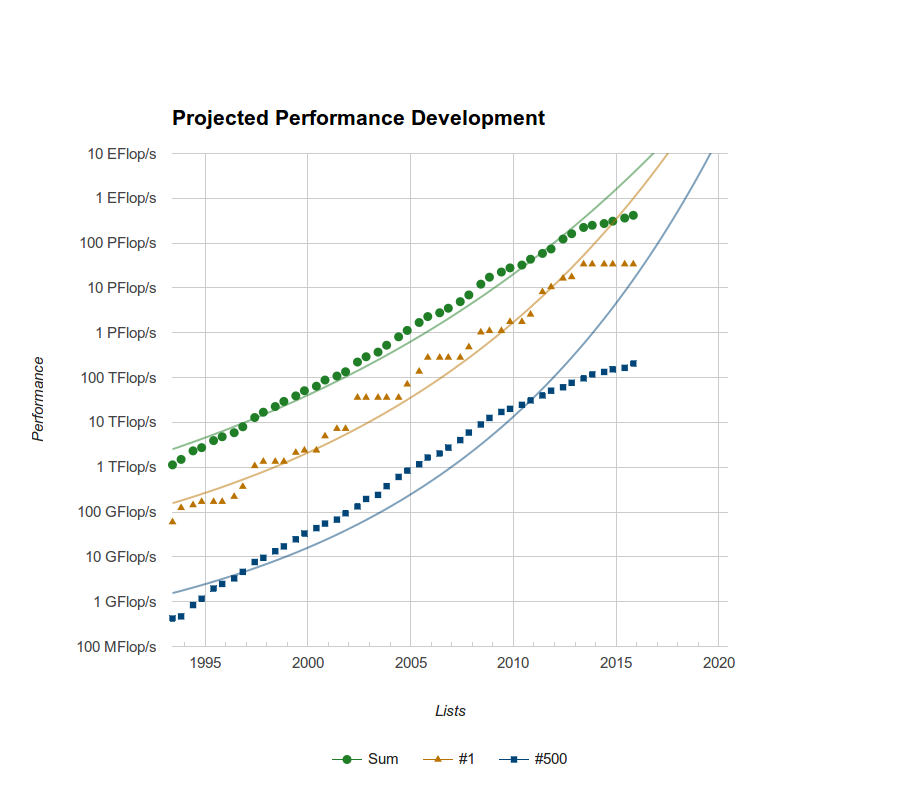
\includegraphics[width=12cm, height=8cm] {PerformanceDevelopment}}
%\caption[Konputagailuen eraginkortasuna.]{www.top500.org, Top: total computing power of top 500 computers. Middle: 1 %computer. Bottom: 500 computer.}
%\label{fig:61}
%\end{figure} 

Konputagailuen eredu aldaketa honen ondorioz, algoritmo azkarrak garatzeko kodearen paralelizazio gaitasunari heldu behar zaio. Programazio paralelo teknikak inplementatzeko, beharrezko da prozesadore berrien hardware arkitekturak nahiz software ingurune berriak ulertzea. Gaia nahiko konplexua izanik, ikuspegi orokorra eman ondoren, gure inplementazioan erabilitako hardware arkitektura eta software teknika zehatzak azalduko ditugu: memoria-konpartitutako sistemak eta OpenMP programazio eredua.

Bi dira, algoritmo azkarrak diseinatzeko erronkak: 
\begin{enumerate}
\item Paralizatzeko pisuko lana identifikatzea.
\item Memoria eta prozesadorearen arteko datu mugimendua gutxitzea. 
\end{enumerate}

Bestalde, inplementazio berrien garapenean optimizatutako liburutegiak erabiltzea komeni da. Horien artean, LAPACK eta BLAS algebra linealeko liburutegiak erabilgarriak izan zaizkigu. Liburutegi hauen gaineko azalpenak emango ditugu.

\section{Eraginkortasuna.}

\subsection*{\textbf{Zein azkarrak dira konputagailuak?}}

Gaur egungo prozesadoreen maiztasun-abiadura hertzetan neurtzen da, hau da,  \emph{makina ziklo segundoko} kopuruaren arabera. Une honetako prozesadoreak gigahertz mailakoak dira.
\begin{description}
\item {Kilo} = mila ($10^3$).
\item {Mega} = milioi ($10^6$).
\item {Giga} = bilioi ($10^9$).
\item {Tera} = trilioi ($10^{12}$).
\item {Peta} = $10^{15}$.
\item {Exa} = $10^{18}$. 
\end{description}

Koma-higikorreko oinarrizko eragiketa bat egiteko ($\oplus,\ominus,\otimes,\oslash$) ziklo gutxi batzuk behar dira. Honek esan nahi du, $1$ GHz-ko prozesadore batek,
$>100.000.000$ koma-higikorreko eragiketa segundoko egiten dituela ($>100$ megaflops).

\paragraph*{\textbf{Adibidea}.} 
Demagun $A,B$ eta $C \ (n \times n)$ dimentsioko matrizeak ditugula eta $C=AB$ matrize arteko biderketa egiteko behar dugun denbora jakin nahi dugula.
\begin{equation*}
c_{ij}=\sum\limits_{i,j=1}^{n} a_{ij}*b_{ji}.
\end{equation*}

\begin{itemize}
\item $c_{ij}$ gai bakoitza kalkulatzeko $n$ biderketa eta ($n-1$) batura egin behar ditugu.
\item $C$ matrizeak $n^2$ osagaia ditu $\Rightarrow$ $O(n^3)$ koma-higikorrezko ariketak exekutatu behar dira.
\end{itemize}

Adibidez, $n=100$ bada $\ \Rightarrow \ n^3=10^{6}$ eragiketa egin behar ditugu. $1$GHz prozesadorean exekutatzeko, $>10^(-2)$ segundo beharko genituzke. 

\paragraph*{} Zientzia konputazioaren eraginkortasuna neurtzeko, koma-higikorreko eragiketa kopurua (\emph{flops}) erabili ohi zen. Problema handia denean, datuen mugimendua koma-higikorreko eragiketak baino garestiagoa da, eta beraz eraginkortasuna eragiketa kopuruaren arabera neurtzea okerra izan daiteke. Kodearen exekuzioa azkartzeko derrigorrezkoa da konputagailuan datuen mugimendua minimizatzea.

\paragraph*{\textbf{Adibidea},} $n=400$ tamainako matrizeak hartzen baditugu, $15,6$ \emph{MB} memoria behar dugu (suposatuz konputagailuaren CACHE memoria baino handiagoa) eta datuen mugimenduaren eragina nabarituko da exekuzio denboran.

\subsubsection*{Timing code.}

Unix \emph{time} agindua erabili daiteke, konputazioen denborak ezagutzeko:

\begin{lstlisting} 
S time ./a.out
<kodearen irteera>

real 0m38.856s
user 0m38.789s
sys  0m0.004s
\end{lstlisting}

Agindu honekin, \emph{./a.out} C programa exekutatuko da eta ondoren, programa exekutatzeko behar izan duen denboraren informazioa pantailaratuko du: \emph{real} hasi eta bukatu arteko denbora (\emph{wall-time}); \emph{user} prozesadoreak gure programa exekutatzen erabili duen denbora (\emph{CPU-time}); \emph{sys} programa exekutatu ahal izateko, sistema eragile lanetan emandako denbora.   

\paragraph*{} C lengoaian badaude, denbora neurtzeko funtzioak. Jarraian, exekuzio denbora (\emph{Wall-time}) eta cpu denborak \emph{CPU-time} nola kalkulatu azaldu dugu.

\begin{lstlisting}[language=C]

#include <time.h>

    time_t  wtime0,wtime1;
    clock_t clock0, clock1; 

    wtime0= time(NULL);
    clock0= clock();

    <neurtu nahi den kodea>

    wtime1= time(NULL);
    clock1=clock();
    
    Wall_time=(wtime1 - wtime0);
    CPU_Time=(clock1 - clock0)/CLOCKS_PER_SEC);

\end{lstlisting}

\emph{Wall-time} deiturikoa izango da algoritmo baten denborak neurtzeko gure irizpidea. Programazio paraleloan, algoritmoen exekuzio denborak egokien neurtzen duen aldagaia da. Dena den, une berean programa bakarra exekutatzea behartuta gaude.       
 

\section{Hardwarea.}

\subsection{Memori hierarkia.}

Lehenik, konputagailuan dauden memoria mota ezberdinen hierarkia azalduko dugu. 
\begin{figure}[h]
\centerline{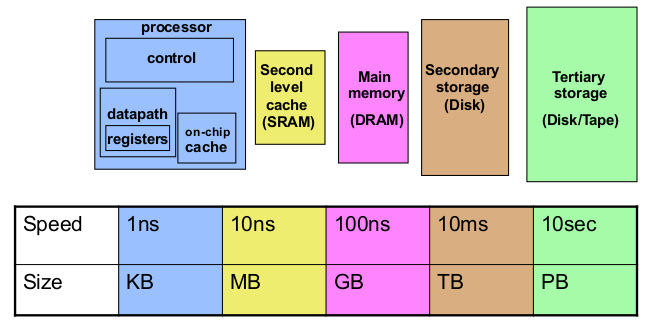
\includegraphics[width=10cm, height=4cm] {MemoryHierarchy}}
\caption{Memoria hierarkia.}
\label{fig:three}
\end{figure} 

\paragraph*{} CPU-k koma-higikorrezko eragiketak egiten ditu: erregistroetatik datuak irakurri, eragiketak egin eta emaitza erregistroetan idazten ditu. Memoria nagusia eta erregistroen artean, 2 edo 3 mailako Cache memoria dugu: lehen Cache memoria (L1) txikiena eta azkarrena da, eta beste mailak (L2,L3,...), handiagoak eta motelagoak. Memoria nagusian, exekutatzen diren programak eta datuak gordetzen dira ($1-4$ GB artekoa). Azkenik, disko gogorrean konputagailuko datu (argazki, bideo,...) eta erabilgarri ditugun programa guztiak gordetzen dira.  

Cache memoria lerroka egituratuta dago eta lerro bakoitza $64$ edo $128$ bytez ($8$ edo $16$ double zenbaki) osatuta dago. Programa batek datu bat behar duenean, memoria nagusitik lerro tamainako datu taldea irakurriko du eta Cachean idatziko ditu. Komunikazio hau minimizatzeko memorian datuak gordetzeko ordenak badu garrantzia. Beraz, datu-egiturak diseinatzen direnean, kontutan hartu behar da une berean beharko diren datuak memorian gertu gordetzea   

\paragraph*{\textbf{Adibidea}.}Badakigunez, C-lengoaian matrizeak lerroka gordetzen dira. Beheko adibidean,  matrizearen lehen osagaia $a(1,1)$ behar dugunean, memoria nagusitik Cachera osagai honetaz gain jarraiko 16 osagaiak ekarriko dira ($a(1,1),a(1,2),\dots,a(1,16)$). Honela, hurrengo $15$ batura egiteko behar ditugun datuak Cachean eskuara izango ditugu memoria irakurketa berririk egin gabe. 

\begin{algorithm}[h]
 \BlankLine
  $int \ n$\;
  $double \ a[n][m]$\;
  \BlankLine
  $sum=0$\;
  \For{$i\leftarrow 1$ \KwTo $n$}
  {
   \BlankLine
    \For{$j\leftarrow 1$ \KwTo $m$}
   {
    \BlankLine 
    $sum+=a(i,j)$\;
   }
 }
 \caption{Memoria atzipena.}
\end{algorithm} 

\begin{equation*}
a=\left(\begin{array}{ccccc}
  1    & 2    & 3    & \dots & 1000 \\
  1001 & 1002 & 1003 &\dots & 2000 \\
  2001 & 2002 & 2003 &\dots & 2000 \\
  \dots & \dots & \dots & \dots & \dots \\
  9001 & 9002 & 9003 &\dots & 10000 \\
  \end{array}\right).  
\end{equation*}

\paragraph*{}CPUk datu bat behar duenean, memoria hierarkian zehar bilatuko du: lehenik $L1$ cachean, ondoren $L2$ cachean,...eta hauetan ez badago, memoria nagusira joko du. Memoria nagusi eta cache memoria arteko irakurketa eta idazketa guzti hauetan,  informazio konsistentzia mantentzeko hainbat arau aurrera ematen dira.  

\subsection{Hardware motak.}

MIMD (Multiple instruction, multiple data) sistemak, guztiz independenteak diren prozesadore multzoak osatzen dituzte. Bi dira MIMD sistema nagusiak: memoria konpartitutako eta memoria banatutako sistemak. Memoria konpartitutako sistemetan, prozesadore guztiek memoria osoa konpartitzen dute eta inplizituki konpartitutako datuen atzipenaren bidez komunikatzen dira. Memoria banatutakotako sistemetan aldiz, prozesadore bakoitzak bere memoria pribatua du eta esplizituki bidalitako mezuen bidez komunikatzen dira.

Hirugarren hardware arkitektura ere aipatuko dugu, general purpose GPU computing (Graphical Processor Unit).
Jokoen eta animazio industrian, grafiko oso azkarrak beharrak bultzatuta  sortutako teknologia da. Oinarrian, imajinak pantailaratzeko prozesagailu asko paraleloan lan egiten dute. Azken hamarkadan, GPU unitate hauek zientzia konputaziora zabaldu dira.  

\begin{figure}[h]
\centerline{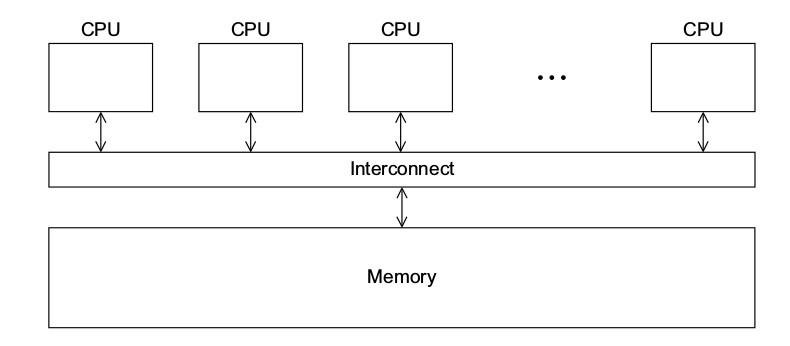
\includegraphics[width=12cm, height=4cm] {SharedMemorySystem}}
\caption{Memoria konpartitutako sistemak.}
\label{fig:61}
\end{figure}  

\begin{figure}[h]
\centerline{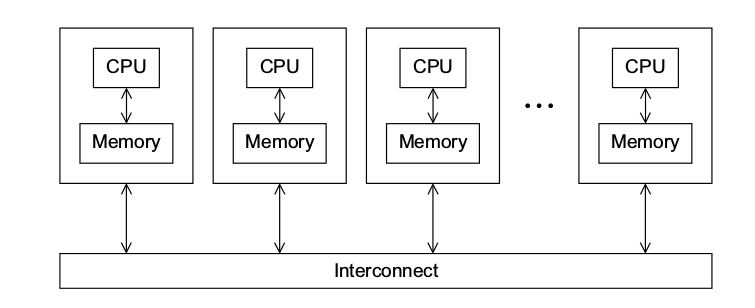
\includegraphics[width=12cm, height=4cm] {DistribuitedMemorySystem}}
\caption{Memoria banatutako sistemak.}
\label{fig:61}
\end{figure}  

\paragraph*{\textbf{Memoria konpartitutako sistemak}.}

Multicore bat edo gehiagoz osatutako sistema dugu. Multicore prozesadore bakoitzak txipean CPU bat baino gehiago ditu. Normalean CPU bakoitzak $L1$ bere cache memoria du. Aipatzeko da, era honetako sistemetan prozesadore kopurua ezin dela nahi adina handitu eta mugatua dela (normalean $\leq 32$ ).

 \begin{figure}[h]
 \centerline{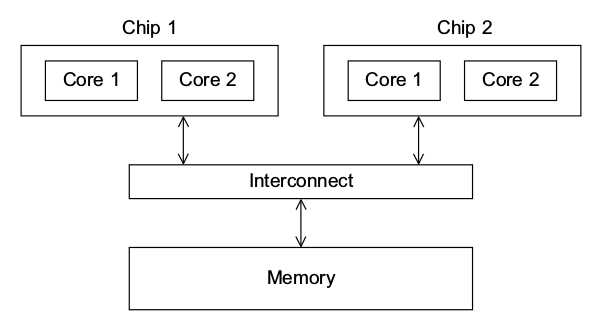
\includegraphics[width=12cm, height=4cm] {SharedMemorySystemUMA}}
 \caption{Memoria konpartitutako sistemak (UMA).}
 \label{fig:61}
 \end{figure}  

\section{Softwarea.}


\subsection{Software liburutegiak.}

Matematika bi software errekurtso nagusienak aipatuko ditugu; BLAS (Basic Linear Algebra Subroutines) eta LAPACK (Linear Algebra Package). Kalitate handiko software orokorrak dira eta hauek erabiltzea abantaila asko ditu: 
\begin{enumerate}
\item Garapen berriak egiteko denbora aurrezten da. 
\item Problema askotan ondo probatutako softwareak dira.
\item Konplexutasun handikoak dira, modu seguruan eta azkarrean exekutatzeko diseinatu direlako. 
\end{enumerate}

Konputagailu hardware bakoitzerako optimizatutako bertsioak daude. Inplementazioa Fortranen egina dago eta datu-motei dagokionez:
\begin{enumerate}
\item S: float ($32$ bit).
\item D: double ($64$ bit).
\item C: complex.
\item Z: complex double.
\end{enumerate}   

\subsubsection*{\textbf{BLAS}.}

BLAS liburutegian, bektore eta matrizeen arteko funtzio estandarrak inplementatuta daude. Hiru mailetan banatuta dago: 

\begin{enumerate}
\item BLAS-1: bektore-bektore eragiketak.

 Adibidez: $y=\alpha*x+y$ , $2n$ flop eta $3n$ irakurketa/idazketa.
 
 Konputazio intentsitatea: $\frac{2n}{3n}=\frac{2}{3}$. 

\item BLAS-2: matrize-bektore eragiketak.

 Adibidez: $y=\alpha*A*x+\beta*x$, $O(n^2)$ flop eta $O(n^2)$ irakurketa/idazketa.
 
 Konputazio intentsitatea: $\approx \frac{2n^2}{n^2}=2$. 
 
\item BLAS-3: matrize-matrize eragiketak.

 Adibidez: $C=\alpha*A*B+\beta*C$, $O(n^3)$ flop eta $O(n^2)$ irakurketa/idazketa.
 
 Konputazio intentsitatea: $\approx \frac{2n^3}{4n^2}=\frac{n}{2}$. 

\end{enumerate}

Azpimarratu, BLAS-1 eta BLAS-2 funtzioen konputazio intentsitatea txikia dela eta beraz, datuen komunikazioa nagusia dela. BLAS-3 aldiz, konputazio intentsitatea handiagoa da eta ezaugarri honi esker, konputagailuaren konputazio gaitasuna ondo aprobetxatu ahal izango da.

\begin{figure}[h]
\centerline{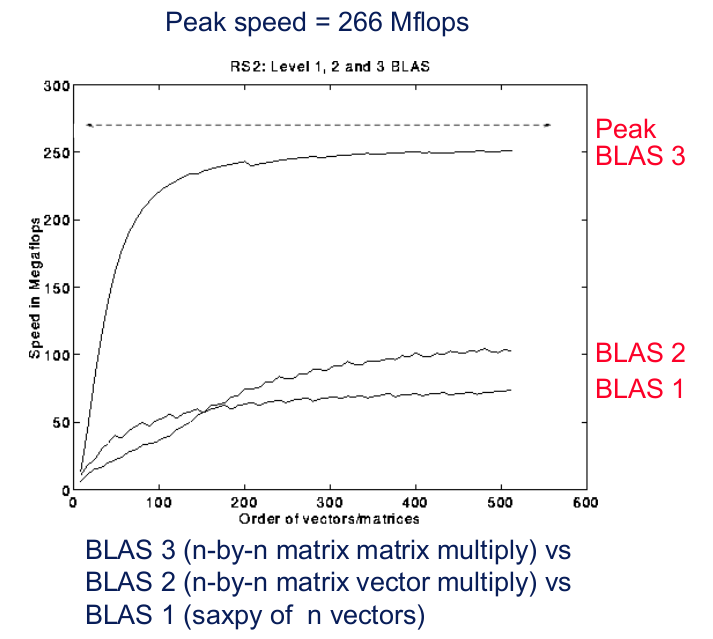
\includegraphics[width=12cm, height=8cm] {BLASSpeed}}
\caption{BLAS speeds.}
\label{fig:61}
\end{figure}    

Fabrikatzaile bakoitzak optimizatutako BLAS liburutegiak (AMD ACML,Intel MKL) dituzte eta beraz, multi-threaded dira.
Beste aukera bat, optimizatutako BLAS instalazioa ATLAS (Automatically Tuned Linear Algebra Software) bidez egitea.    

\subsubsection*{\textbf{LAPACK}}.

Zenbakizko aljebra linealaren liburutegia da.

\begin{enumerate}
\item Sistema linealak: $AX=b$.
\item Least Square: choose $x$ to minimize $\|Ax-b\|$.
\item Eigenvalues.
\item Balio singularren deskonposaketa (SVD).
\end{enumerate}

Posible den guztietan, BLAS-3 funtzioetan oinarritzen da.

\subsection{Programazio paraleloa.}

C-lengoaia programazio paraleloan erabiltzeko, lengoaiaren bi extensio dira nagusienak: bata memori-banatutako sistemetarako diseinatuta  MPI (Message-Passing Inteface) eta bestea, memoria-konpartitutako sistemetarako diseinutakoa OpenMP (Open Specifications for MultiProcessing). MPI datu moten definizio, funtzio eta makroen liburutegia da. OpenMP liburutegia bat  eta C konpiladorearen aldaketa batzuk. OpenMP erabili dugu gure inplementaziorako eta jarraian honi buruzko idei nagusienak emango ditugu.

\paragraph*{\textbf{OpenMP}.}

Memoria konpartitutako programazio paraleloaren estandarra dugu. 
Programazioan paralelizazio kontrola, "fork-join" modeloa jarraituz egiten da.

\begin{enumerate}
\item OpenMP programen hasieran prozesu bakarra dago, hari (thread) nagusia. 
\item FORK: hari nagusiak hari talde paraleloa sortzen du.
\item JOIN: hariak kode paraleloa bukatzen dutenean, behin sinkronizatuta amaitzen dute eta hari nagusiak bakarrik jarraitzen du.
\end{enumerate}

% \begin{figure}[h]
% \centerline{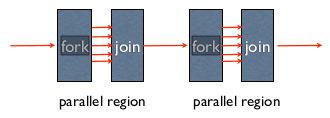
\includegraphics[width=10cm, height=3cm] {ForkJoin}}
% \caption{Fork-Join.}
% \label{fig:61}
% \end{figure}  
 
 \begin{figure}[h]
 \centering
 \subfloat[Fork-Join.]{
 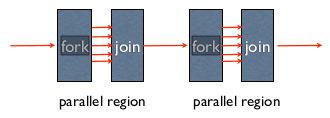
\includegraphics[width=.500\textwidth]{ForkJoin}
 }
 \subfloat[Fork-Join.]{
 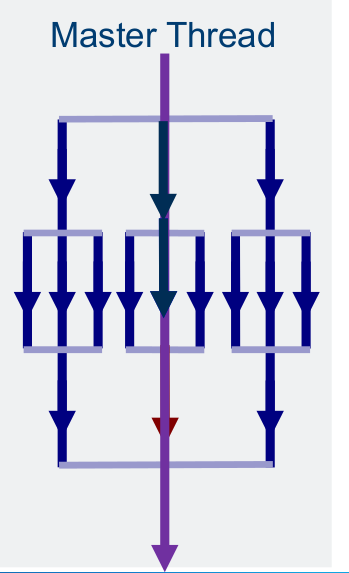
\includegraphics[width=.200\textwidth]{OpenMP1}
 }
  \caption[OpenMp programazio modeloa.]{\small OpenMp programazio modeloa.}
 \label{fig:forkjoin}
 \end{figure}

Aldagai batean (threadcount) paralelizazioan zenbat hari erabili adierazten da eta ohikoa izaten da hari bat prozesadore bakoitzeko sortzea.  Konpilazio direktiben bidez,  paralelizazioa nola exekutatu behar den zehazten zaio.

\paragraph*{\textbf{Adibidea}}.

\begin{lstlisting}[language=C]
#    pragma omp parallel for num_threads(thread_count) 
     for (i = 0; i<n; i++)
     {
       ! Aginduak 
     }
\end{lstlisting}

OpenMP Version 4.5.	

gcc -v (gcc version 4.8.4 (Ubuntu 4.8.4-2ubuntu1~14.04.3))

A number of compilers from various vendors or open source communities implement the OpenMP API:

\begin{enumerate}
\item From GCC 4.7.0, OpenMP 3.1 is fully supported. 

\item From GCC 6.1, OpenMP 4.5 is fully supported in C and C++.

\end{enumerate}   


\subsection{Konpiladorea.}

\subsubsection*{Sarrera.}

Erabiliko dugun konpiladorea,

\begin{enumerate}

\item \emph{gcc} - \emph{GNU} open source compiler.

\begin{lstlisting}
$ gcc -v
$ gcc version 4.8.4 (Ubuntu 4.8.4-2ubuntu1~14.04.3) 
\end{lstlisting}

\item Several comercial compilers also are avalaible.

\end{enumerate}


C11 (formerly C1X) is an informal name for ISO/IEC 9899:2011,[1] the current standard for the C programming language.It replaces the previous C standard, informally known as C99. This new version mainly standardizes features that have already been supported by common contemporary compilers, and includes a detailed memory model to better support multiple threads of execution.

gcc requires you specify -std=c99 or -std=c11


\paragraph*{Optimizations} (-Olevel).
        
Optimizes the code for execution speed according to the level specified by level , which can be 1, 2, or 3. If no level is specified, as in –O , then 1 is the default. Larger numbers  indicate higher levels of optimization.

-O2 (default) Optimize for code speed. This is the generally recommended optimization level. -O3 Enable -O2 optimizations and in addition, enable more aggressive optimizations such as loop and memory access transformation, and prefetching. 

Every compiler offers a collection of standard optimization options (-O0,-O1,. . . ).  However, all compilers refrain from most optimizations at level -O0, which is hence the correct choice for analyzing the code with a debugger. At higher levels, optimizing compilers mix up source lines, detect and eliminate “redundant” variables, rearrange arithmetic expressions, etc.,      

\subsubsection*{Konpilazioa.}

\paragraph*{Oinarrizko erabilpena.}

\begin{enumerate}
\item Compiles and links and creates an executable adibidea.exe.
\begin{lstlisting}[language=C]
$ gcc adibidea.c -o adibidea.exe
\end{lstlisting}

\begin{lstlisting}[language=C]
$ ./adibidea.exe
\end{lstlisting}

\item Compile and link steps.

\begin{lstlisting}[language=C]
$ gcc adibidea.c  # creates adibidea.o
$ gcc adibidea.o -o adibidea.exe
\end{lstlisting}

\end{enumerate}

\begin{lstlisting}[language=C]
gcc -O2 -Wall -std=c99 -fno-common adibidea.c
\end{lstlisting}

\subsubsection*{Makefile.}

A common way of automating software builds and other complex tasks with dependencies.

A Makefile is itself a program in a special language.

\paragraph*{Adibidea.}
Demangun programa bat hiru fitxategieten banatuta dugula,

\begin{lstlisting}[language=C]
/*file: main.c*/
void main()
{
    printf("Main program");
    sub1();
    sub2();
}
\end{lstlisting}

\begin{lstlisting}[language=C]
/*file: sub1.c*/
void sub1()
{
    printf("sub1");
}
\end{lstlisting}

\begin{lstlisting}[language=C]
/*file: sub2.c*/
void sub2()
{
    printf("sub2");
}
\end{lstlisting}

Programa exekutagarria lortzeko makefile fitxategia,

\begin{lstlisting} [language=C]
main.exe: main.o sub1.o sub2.o
	      gcc main.o sub1.o sub2.o -o main.exe
main.o: main.c
        gcc -c main.c
sub1.o: sub1.c
        gcc -c sub1.c        
sub2.o: sub2.c
        gcc -c sub2.c        
\end{lstlisting}

\begin{lstlisting}
$ make main.exe
gcc -c main.c
gcc -c sub1.c
gcc -c sub2.c
gcc main.o sub1.o sub2.o -o main.exe
\end{lstlisting}

Typical element in the simple Makefile:

\begin{lstlisting}
target: dependencies
>TAB>  command(s) to make the target
\end{lstlisting}

Typing "make target" means:
\begin{itemize}
\item Make sure all dependencies are update (those that are also targets).
\item If target older than any dependency, recreate it using specified commands.
\item The rules are applied recursively.
\end{itemize}

\paragraph*{\textbf{MakefileV2}}

\begin{lstlisting} [language=C]

CC = /usr/bin/gcc
FLAGS=-O2 -Wall -std=c99 -fno-common 
OBJECTS=  main.o sub1.o sub2.o
.PHONY: clean help

main.exe: $(OBJECTS)
	      ${CC} $(OBJECTS) -o main.exe
	      
%.o: %.c
     ${CC} ${FLAGS} -c $<	      
	      
clean:
     rm -f $(OBJECTS) main.exe

help:
    @echo "Valid targets;"
    @echo " main.exe"
    @echo " main.o"
    @echo " sub1.o"
    @echo " sub2.o"
    @echo " clean"
             
\end{lstlisting}


\section{Kode Optimizazioak.}

Applications have two general challenges:
\begin{enumerate}
\item Numerical Method.

Performance required computation the shortest account of time.

\item. Computer Program.

Express the algorithm as fast computer problem, you have realized computer hardware eficiently.

\end{enumerate}

Optimization areas are:
\begin{enumerate}
\item Vectorization.
\item Paralelization.
\item Memory trafic control.
\end{enumerate}

Optimization areas:
\begin{enumerate}
\item scalar optimization (compiler friendly practices).

\item vectorization (must use 16 or 8 wide vectors).

\item multi-threading (must  scale to $100+$ threads).

\item memory access (streaming acces).

\item communication (offload, MPI traffic control).

\end{enumerate}


\subsection*{Scalar Tuning and General Optimization.}

Optimization of scalar arithmetics.

One of the most important scalar optimizazion techincs is  \textbf{strength reduction} : replace expensive operation for less expensive operations.

\begin{figure}[h]
 \centerline{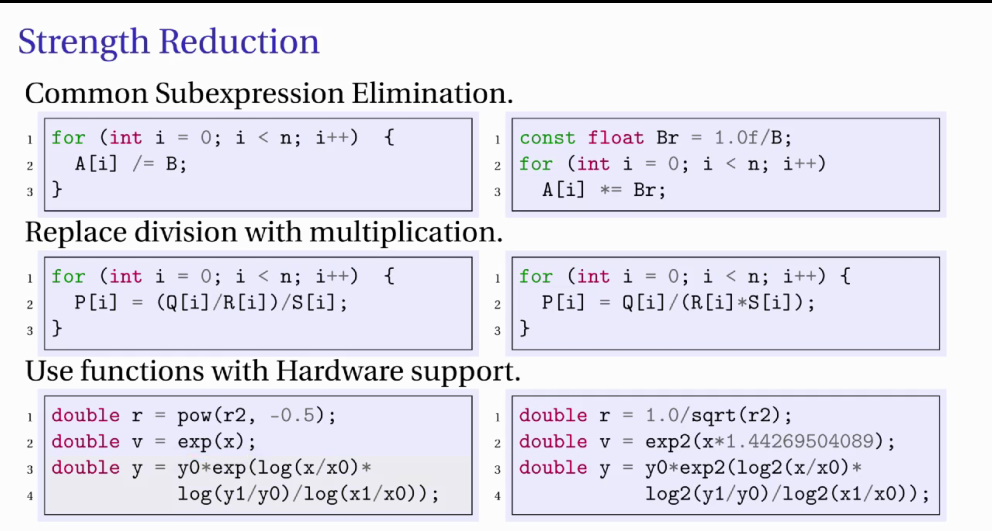
\includegraphics[width=12cm, height=4cm] {Optimization_Strength_Reduction}}
 \caption{Optimization.}
 \label{fig:61}
\end{figure}  

\paragraph*{} Precision control.

\begin{enumerate}
\item Precision Control for transcendental functions.

\item Floating-point semantics.

\item Consistency of precision: constants and constants.

Using incorrect function names in the single precsion is a common mistake

\end{enumerate}

\subsection*{Optimization of vectorization.}

\begin{enumerate}

\item Preferably unid-stride access to data.
Very important step in the optimization.

Artikulua "Auto-Vectorization with the Intel Compilers".

Most CPU architectures today include Single Instruction Multiple Data (SIMD) parallelism in the form
of a vector instruction set. Serial codes (i.e., running with a single thread), as well as instruction-parallel cal-
culations (running with several threads) can take advantage of SIMD instructions and significantly increase
the performance of some computations. Each CPU core performs SIMD operations on several numbers (in-
tegers, single or double precision floating-point numbers) simultaneously, when these variables are loaded
into the processor’s vector registers, and a vector instruction is applied to them. SIMD instructions include
common arithmetic operations (addition, subtraction, multiplication and division), as well as comparisons,
reduction and bit-masked operations (see, e.g., the list of SSE 2 intrinsics). Libraries such as the Intel Math
Library provide SIMD implementations of common transcendental functions, and other libraries provide
vectorized higher-level operations for linear algebra, signal analysis, statistics, etc.

\item Data Alignment and Padding.

An important consideration for efficient vectorization is data alignment.


\end{enumerate}

\subsection*{Multi-threading.}

Do you have enough parallelism in your code? 

Expanding iteration space, if it is no enough iterations in parallel loop.

Three layers of parallelism: MPI processes, OpenMP threads, vectorization.


\subsection*{Memory access.}

Memory access and Cache utilization.

loop tiling technics

\begin{figure}[h]
 \centerline{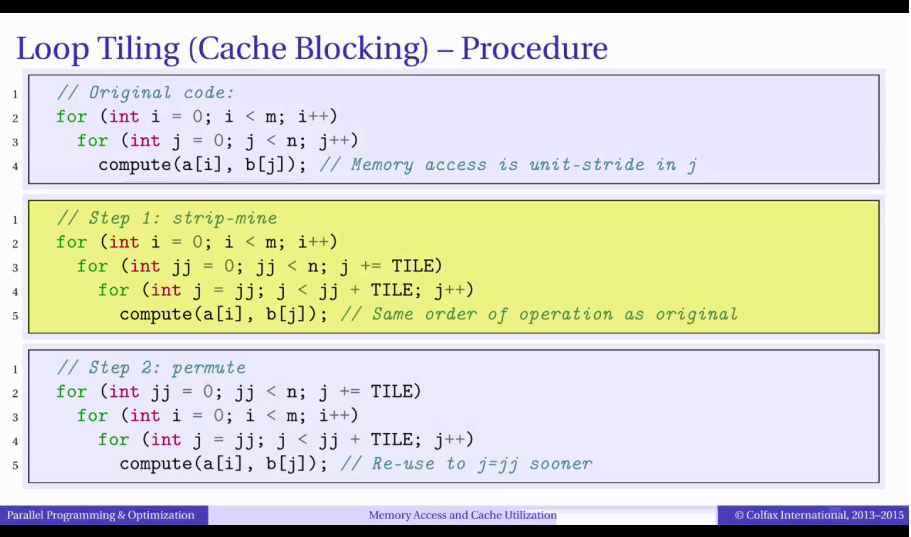
\includegraphics[width=12cm, height=4cm] {Optimization_LoopTiling}}
 \caption{Optimization.}
 \label{fig:61}
\end{figure}  

\section{Laburpena.}

Best practices for code vectorization and parallelization, and additional tips and tricks.

Algoritmo bat inplementatzen dugunean kontutan hartu beharrekoa:

\begin{enumerate}

\item Lerro edo zutabe araberako iterazioak exekuzio denboran eragin handia du.

\item Kodea garbia eta ulergarria mantendu behar da.

\item Badaude kodearen exekuzio denboraren analisia egiteko tresnak (adibidez gprof). Algoritmoaren funtzio bakoitzaren exekuzio denborari buruzko informazio erabilgarria lortuko dugu. Zenbait gauza modu sinplean azkartu daitezke baina zenbait beste gauza azkartzeko esfuertzu handia eskatu dezake.

\item Optimizatutako beste hainbat kode erabiltzea komenigarria da. LAPACK aljebra lineal paketea Fortran eta C-lengoaitetatik deitu daiteke. Eraberean, LAPACKek BLAS subrutinak erabiltzen ditu.  Subrutinak hauek matrizen arteko biderketak, "inner product", ... BLAS konputagailu arkitektura ezberdinetarako optimizatutako bertsioak daude.
 

\end{enumerate}


%\chapter{Eguzki-sistemaren integraziorako metodoak (review).}

\section{Sarrera.}

\section{Efemerideak.}

Hiru dira planetak efemerideak,

\begin{enumerate}
\item Jet Propulsion Laboratory, DE (Development Ephemerides).

      Integrazio tartea: $1550-2650$.

      Zenbkizko metodoa: "DIVA" (Krogh,1997).A variable order Adams method.
      
      Doitasuna: "QIVA" a quaruple precision of "DIVA" : the equations of motion , the newtonian part is computed in quadruple precision; all of the rest are computed in double precision.

\item Paris Observatory, INPOP (Intégrateur Númerique Planétaire de l'Observatoire de Paris).
      
      Integrazio tartea: .
      
	  Zenbakizko metodoa: The integrator is an Adams-Cowell method with fixed step-size.
	  
	  Doitasuna:  the programming is done in C language, thus allowing to use the extended precision (80 bits). 
	  Integrating in quadruple precision would of course reduce the round off error in a very large amount, but the
	  CPU time is about 15 time larger than for double precision arithmetic (or extended arithmetic) on our machine
	  (Itanium II with Intel C++ compiler). Nevertheless, it was possible to obtain an additional order of magnitude im-
	  provement by using a single addition in simulated quadruple precision in the corrector step with a very small over-
	  head.
	  
	  Hardware: Intel Itanium II processors.
	  
\item St. Petersburg, EPM (Ephemerides Planets-Moon).
      
      Integrazio tartea: .
      
      Zenbakizko metodoa: Everhart. Implicit RK method (Gauss-Radau).
      (An efficient integrator that uses Gauss-Radau Spacings)
      
      Doitasuna: double precision. The change of ERA system integrator (19 decimal digits instead of 15 ones) with the aim to reduce the round-off error. (Extended precision).
      
\end{enumerate}

\paragraph{Influence of the methods of constructing ephemerides...}
It is obvious that such ephemerides in themselves must have 128 bits, that is, comprise the coefficients calculated with quadruple precision.


\section{Eguzki-sistemaren integrazio luzeak.}

A.Morbidellik \cite{Morbidelli2002} eguzki-sistemaren zenbakizko integrazioen algoritmoen garapenaren azterketan, gaia hauek sailkatzen ditu:

\begin{enumerate}

\item The classical period.

$90$. hamarkada hasiera arte,  

\item The symplectic period.

\item The statistic period.

\item The planetary accretion period. 

\end{enumerate}


Wisdomek eta Holmanenek bere lanean \ycite[1991]{Sussman1992},  eguzki-sistemaren epe luzeko simulazioetarako integratzaile  sinplektikoen erabilerak arrakasta izan zuen. N-planeta eta masa nagusiko gorputza bat dugula kontsideratuta, problemaren Hamiltondarra bitan banatu zuten:  Hamiltondar Kleperiarra eta interakzioen Hamiltondarra. Metodo honetan, Hamiltondar bakoitzaren soluzioa tartekatuz, problema osoaren ebazpena kalkulatuko da. 

Wisdom eta Holmanen inplementazioak ez ditu kolisio gertuko egoerak onartzen. Arazo hau gainditzeko, urteetan zehar algoritmo honen hainbat aldaera proposatu dira: Levinson eta Duncan-ek \ycite[1994]{Levison1994}  \emph{SWIFT} softwarea garatu zuten;  Duncan, Levinson eta Lee-k \ycite[1998]{Duncan1998} \emph{SYMBA} softwarea garatu zuten; Chambers-ek \cite{Chambers1999} \emph{MERCURY} softwarea garatu zuen. Berriki, Hernandez eta Bertschinger-ek \ycite[2015]{Hernandez2015} garapen berri bat proposatu dute.

Koordenatu sistema aukera ezberdinak erabili dira Hamiltondarraren banaketa lortzeko. Jacobi koordenatuak eta koordenatu Heliozentrikoak erabili ohi dira bakoitzak bere abantaila eta desbaintailekin.

Problema integratzeko oinarrizko metodoa \emph{leapfrog} metodoa dugu. Metodo hau 2 ordeneko da. Orden altuagoko splitting eskemak : McLachlan \ycite[1995]{McLachlan1995}, Laskar eta Robutel \cite[2001]{Laskar2001}, Blanes \cite{Blanes2013}.

\section{Laburpena.}   
       


\part{Ekarpenak.}
\chapter{IRK: Puntu-Finkoa.}

\section{Sarrera.}


Puntu-finkoan oinarritutako \emph{non-stiff} sistema Hamiltondarren zenbakizko integraziotarako IRK metodoaren inplementazioa proposatuko dugu. Zientzian, konputazioak koma-higikorreko aritmetikarekin egien direnez, biribiltze erroreak soluzioen doitasuna mugatzen du. Hortaz, inplementazioa epe luzeko doitasun altuko zenbakizko integrazioetarako aplikagarria izateko, biribiltze errorearen eraginak txikia izan behar du. Era berean, integrazioan zehar biribiltze errorearen estimazioa ezagutzea interesgarria da. 

Integrazioaren exekuzio denborak onargarriak izan daitezen , honako aurrebaldintza finkatu dugu: ekuazio diferentzialaren eskuin aldeko funtzioaren sarrera eta irteera argumentuak makina zenbakiak izatea, hau da, konputagailuan hardware bidezko exekuzioa (azkarra) duen koma-higikorreko aritmetika erabiltzea. Gaur-egun, zientzia-konputazioan $64$-biteko koma-higikorreko aritmetikarekin (\emph{double} datu-mota) lan egiten da eta beraz, praktikan erabiltzaileak ekuazio diferentziala datu-mota honetan zehaztuko duela suposatuko dugu. 
 
Lehenengo Hairer-en inplementazioa  \cite{Hairer2008} aztertuko dugu. Ondoren, IRK inplementazioa hobetzeko gure proposamenak azalduko ditugu. Azkenik, zenbakizko gure inplementazioaren emaitzak erakutsiko ditugu.

\section{Hairer-en inplementazioa.}

Gure abiapuntua, Haier-ek \cite{Hairer2008} proposatutako inplementazio hartu dugu.  
Lan honetan, IRK metodo sinplektikoaren puntu-finkoaren inplementazio estandarrean biribiltze errorearen garapen okerraz jabetu ziren eta gainera, metodo sinplektiko esplizituetan agertzen ez zena. Hauen ustez, bi ziren errore honen jatorriak:

\begin{enumerate}
\item Integrazioan $a_{ij}, b_i \in \mathbb{R}$ koefiziente zehatzak erabili ordez, biribildutako $\tilde a_{ij},\tilde b_i \in \mathbb{F}$ erabiltzeak, aplikatutako IRK metodoa zehazki sinpletikoa ez izatea eragiten du.
\item Puntu-finkoaren geratze irizpide estandarra dela eta, urrats bakoitzean errore sistematikoa gertatzen da.
\begin{equation*}
\triangle ^{[k]} = \max_{i=1,\dots,s}\|Y_i^{[k]}-Y_i^{[k-1]}\|_{\infty} \le \delta
\end{equation*}

\end{enumerate}    

\paragraph*{}Arrazoi hauek aztertu ondoren, honako konponbideak proposatu zituzten:

\begin{enumerate}
\item Doitasun handiagoko koefizienteak erabili, hauetako bakoitza bi koma-higikorreko koefizienteen batura kontsideratuz,
\begin{equation*}
a_{ij}= a^{\ast}_{ij}+\tilde a_{ij}, \ b_i= b^{\ast}_i+\tilde b_i
\end{equation*} 
non $a^{\ast}_{ij}>\tilde a_{ij}$ eta  $b^{\ast}_i>\tilde b_i$ diren. 


\paragraph*{}Zehazki era honetan kalkulatu daitezke,
\begin{equation*}
a^{\ast}_{ij}=(a_{ij} \otimes 2^{10}) \oslash 2^{10},\ \ \tilde a_{ij}= a_{ij}\ominus a^{\ast}_{ij}.
\end{equation*}


\item Iterazioak geratu, definitutako norma txikitzeari uzten dionean.
\begin{equation*}
\triangle^{[k]} = 0 \ \ or \  \triangle^{[k]} \geqslant \triangle^{[k-1]}.
\end{equation*}
  	 	
\end{enumerate}

Hairer-ek bere \emph{Fortran} inplementazioa eskuragarri du (\href{http://www.unige.ch/~hairer/preprints.html}{Fortran kodea}). Jarraian Hairer-en algoritmoa laburtu dugu (alg.\ref{alg:Hairer-IRK}). Aipatutako hobekuntzaz gain, batura konpensatua erabiltzen duela azpimarratu nahi dugu (notazioa sinplifikatze aldera $Y_{n,i}$ gaiaren ordez, $Y_i$ adierazpena erabiliko dugu).
 

\begin{algorithm}[h!]
 \BlankLine
  $e=0$\;
  \For{$n\leftarrow 0$ \KwTo ($endstep-1$)}
  {
   \BlankLine
   $k=0$\;
   $Y_{i}^{[0]}=y_n+h \ c_i \ f(y_n) $\; 
   \BlankLine
   \While{ ($\triangle^{[k]} \ != 0 \ \ and \  \triangle^{[k]} < \triangle^{[k-1]}) $}
   {
    \BlankLine 
    $k=k+1$\;
    $F_{i}^{[k]}=f(Y_{i}^{[k-1]}) $\;
    $Y_{i}^{[k]}=y_n+ h \ \big(\sum\limits_{j=1}^{s} a^{\ast}_{ij} F_{j}^{[k]} \big) 
                          + h \ \big(\sum\limits_{j=1}^{s} \tilde a_{ij} F_{j}^{[k]} \big)$\; 
    $\triangle ^{[k]} = \max_{i=1,\dots,s}\|Y_{i}^{[k]}-Y_{i}^{[k-1]}\|_{\infty}$\;
   }
   \BlankLine
    $\delta^{\ast}_{n}=h \ \big(\sum\limits_{i=1}^{s} b^{\ast}_i F_{i}^{[k]} \big)$\;
    $\tilde{\delta}_{n}=h \big(\sum\limits_{i=1}^{s} \tilde b_i F_{i}^{[k]} \big)$\;
    $ee=\delta^{\ast}_{n}+e$\;
    $yy=y_n+ee$\;
    $ee=(y_n-yy)+ee$\;
    \BlankLine
    $ee=\tilde{\delta}_{n}+ee$\;
    $y_{n+1}=y_{n}+ee$\;
    $e=(yy-y_{n+1})+ee$\;            
   \BlankLine
 }
 \caption{Hairer IRK} \label{alg:Hairer-IRK}
\end{algorithm}


\section{Gure inplementazioa.}

IRK metodoaren puntu-finkoaren inplementazioan lau proposamen berri egin ditugu. Lehen bi proposamenak  Hairer-ek bere lanean proposatutako konponbideen hobekuntzak dira. Batetik, IRK-ren birformulazio bat erabiliz, IRK metodoaren koma-higikorreko koefizienteak sinplektizidade baldintza zehazki betetzea lortuko dugu. Bestetik, geratze irizpidean arazo batzuk topatu ditugu eta arazo hauek gainditzen dituen geratze irizpide sendoagoa garatu dugu. Beste bi proposamenak dagokionez, bata batura-konpensatuari erlazionatuta dago eta bestea biribiltze errorea monitorizatzeko proposamena da.

Bestalde kapitulu honen bukaeran, interpolazio bidezko atalen hasieraketa azalduko dugu. Bukatzeko, gure algoritmoa azalduko dugu.  

\subsection{Metodoaren birformulazioa (1.proposamena).}

IRK metodoa definitzen duten $a_{ij},b_i$ koefizienteak, biribildutako $\tilde a_{ij},\tilde b_i \in \mathbb{F}$ ordezkatzerakoan, sinpletizide baldintza ez da beteko,
\begin{equation} \label{eq:61}
b_{i}a_{ij}+b_{j}a_{ji}-b_{i}b_{j}=0, \ \ 1 \leqslant i,j \leqslant s.
\end{equation}  
  
Arazo hau gainditzeko asmoarekin, IRK metodoa era honetan birformulatuko dugu,
\begin{align}
\label{eq:62}
Y_{n,i}&=y_n+ \sum\limits_{j=1}^{s} \mu_{ij} L_{n,j},  \ \ L_{n,i}=hb_if(Y_{n,i}), \ \ i=1,\dots,s,\\
y_{n+1}&=y_n+\sum\limits_{i=1}^{s} L_{n,i},
\end{align}
non 
\begin{equation*}
\mu_{ij}=a_{ij}/{b_j}, \ \ 1 \le i,j \le s.
\end{equation*}

Eta sinplekzidade baldintza modu honetan berridatziko dugu,
\begin{equation}
\mu_{ij}+\mu_{ji}-1=0, \ \ \ 1 \le i,j \le s.
\end{equation}

Formulazio berri honek  estandarrarekiko duen abantaila handiena , sinplektizidade baldintzan biderketarik agertzen ez denez,  baldintza hau betetzen duten $\tilde \mu_{ij} \in \mathbb{F}$ koefizienteak aurkitzeko bidea errazten zaigula da. Honako izango da koefiziente hauek finkatzeko bidea:

\begin{enumerate}
\item $\mu_{ij}$ koefizienteak.

Batetik $s$-ataleko Gauss metodoetan, diagonaleko koefizienteek ($\tilde{\mu}_{ii}:=1/2, \ i=1,\dots,s$) koma-higikorreko adierazpen zehatza dute.

Bestetik gainontzeko koefizienteak erabakitzeko, lehengo $\tilde{\mu}_{ij}:=fl(\mu_{ij}), \ 1 \le j < i \le s$ koefizienteak balioekin finkatuko ditugu. Eta bigarrenik, $\tilde{\mu}_{ji}:=1-\tilde{\mu}_{ij} , \ 1 \le j < i \le s$ koefizienteei balioa esleituko diegu;  $1/2 < |\mu_{ij}| <2$ denez, eta Sterbenz-en Teoremaren (ikus. \ref{eq:4311}) arabera  $1-\tilde{\mu}_{ij}$ koma-higikorreko adierazpen zehatza du. 

Beraz, hauek ditugu simplektizitate baldintza zehazki betetzen duten koma-higikorreko $\tilde{\mu}_{ij}\in \mathbb{F}$ koefizienteak.   
\begin{equation}
\tilde{\mu}=\left(\begin{array}{cccc}
    1/2       & 1-fl(\mu_{21}) & \dots & 1-fl(\mu_{s1})      \\
    fl(\mu_{21})      & 1/2    & \dots & 1-fl(\mu_{s2})      \\
    \vdots            & \ddots         &       & \vdots      \\
    fl(\mu_{s1})      & fl(\mu_{s2})   & \dots & 1/2          \\ 
     \end{array}\right)
\end{equation}

\item $b_{i}$ koefizienteak.

Gure inplementazioan, $hbi$ koefizienteak aurre-kalkulatuko ditugu. Batetik, koefiziente hauek simetrikoak direla eta bestetik, $\sum\limits_{i=1}^{s} hb_i=h$ berdintza bete behar dela kontutan hartuz,
\begin{eqnarray}
hb_1=hb_s:= h - \sum\limits_{i=2}^{s-1} hb_i
\end{eqnarray}

\item $y_{n+1}=y_n+\sum\limits_{i=1}^{s}L_{n,i}$ baturan, batugaien ordena.

Batugaien ordenak, batura errekurtsiboen emaitzaren doitasunean eragina du \cite{Higham2002}. Zenbaki positiboen batura dugunean, egokiena magnitude txikienetik handienerako batugaien ordena erabiltzea da. Horregatik, honako batura $y_{n+1}=y_n+\sum\limits_{i=1}^{s} hb_i f(Y_{n,i})$ irizpide honi jarraituz, $b_i$ koefizienteen txikienetik handieneko ordenaren arabera kalkulatuko dugu. 

\end{enumerate}

\subsection{Geratze irizpidea (2.proposamena).}

Ekuazio inplizituaren (\ref{eq:62}) soluzioaren hurbilpena lortzeko puntu-finkoko iterazioa era honetan definituko dugu. Iterazioaren abiapuntua $Y_i^{[0]}$  finkatu eta $k=1,2,\dots$ iterazioetarako $Y_i^{[k]}$ hurbilpenak lortu dagokigun geratze irizpidea bete arte.
%\begin{equation}
%L_i^{[k]}=hb_if(Y_i^{[k-1]}), \ \ Y_i^{[k]}=y_n+\sum\limits_{j=1}^{s} \mu_{ij} L_j^{[k]}
%\end{equation}

\begin{algorithm}[H]
 \For{ (k=1,2,\dots)}
  {
   $L_i^{[k]}=hb_if(Y_i^{[k-1]}) $\;
   $Y_i^{[k]}=y_n+\sum\limits_{j=1}^{s} \mu_{ij} L_j^{[k]} , \ \  i=1,\dots,s $\; 
   }
 \caption{Puntu-finkoko iterazioa.}
\end{algorithm}
 
\paragraph*{}IRK metodoaren inplementazio estandarrean geratze irizpidea honakoa da,
\begin{equation*}
\triangle^{[k]}=(Y_1^{[k]}-Y_1^{[k-1]},\dots,Y_s^{[k]}-Y_s^{[k-1]}) \in \mathbb{R}^{sd},
\end{equation*} 
\begin{equation}
\|\triangle^{[k]}\| \le tol
\end{equation}
non $\|.\|$ aurre-finkatutako bektore norma eta \emph{tol} tolerantzia errorea den . Tolerantzia txikiegia aukeratzen bada, gerta daiteke tolerantzia hori ez lortzea eta infinituki iterazioak exekutatzea. Baina tolerantzia ez bada behar adina txikia  aukeratzen, iterazioa puntu-finkora iritsi aurretik geratuko da eta lortutako $Y_i^{[k]}$ hurbilpenak biribiltze errorea baino errore handiago izango du.

Hairer-ek proposatu zuen geratze irizpidea gogoratuko dugu; $\triangle^{[k]} = 0$ (puntu-finkora iritsi delako) ;  edo   $\triangle^{[k]} \geqslant \triangle^{[k-1]}$ (biribiltze errorea nagusi delako). Orokorrean, geratze irizpide honek ondo funtzionatzen du baina esperimentalki zenbait kasuetan, iterazioak goizegi geratu direla konprobatu dugu. Gure iritziz, honen arrazoia da $\triangle^{[k]} \geqslant \triangle^{[k-1]}$ biribiltze errorea nagusia dela adierazten duen arren, badago $j \in \{1,\dots,sd\}$ osagairik,   $|\triangle_j^{[k]}| < |\triangle_j^{[k-1]}|$ hobetzeko tartea duena. 

Gure proposamena azaldutako arazoari soluzioa emateko, iterazioak jarraitzea honako baldintza betetzen den artean,
\begin{equation}
\exists j \in \{1,\dots,sd\} \ , \ |\triangle_j^{[1]}| >|\triangle_j^{[2]|}>\dots>|\triangle_j^{[k]}|>0.
\end{equation}


\subsection{Biribiltze errorea gutxitzeko teknikak (3.proposamena).}

Koma higikorreko aritmetika atalean (ikus \ref{sec:4.4}.atala) birbiltze errorea gutxitzeko bi teknika aipatu genituen: batura konpensatua eta biderketaren biribiltze errorea jasotzeko modua. Batetik, IRK metodoetan batura konpensatuaren aplikazio estandarra hobetzeko proposamena azalduko dugu eta bestetik, biderketaren biribiltze errorea nola aplikatu urratsaren gehikuntzan.   

\subsubsection*{Batura konpensatua.}
Integrazioaren zenbakizko soluzioa  $y_{n+1} \approx y(t_{n+1})$  lortzeko, urrats bakoitzean honako batura dugu,
\begin{equation*}
y_{n+1}=y_{n} + \phi(y_{n,h}), \ \ n=0,1,2,\dots.
\end{equation*}   

IRK metodoetan, $\phi: \mathbb{R}^{[d+1]} \rightarrow \mathbb{R}^d$ gehikuntza,
\begin{equation*}
\phi(y_{n,h})=\sum\limits_{i=1}^{s} L_{n,i},
\end{equation*}
non $L_{n,i}$ ($i=1,\dots,s$) inplizituki definitzen den.

\paragraph*{}Urrats askotako integrazioetan, batura honetan gertatutako biribiltze erroreak doitasun galera garrantzitsua sortzen du. Beraz, zenbakizko integrazioetan biribiltze errorea gutxitzeko  batura konpensatu estandarra aplikatzea oso erabilgarria zaigu (ikus \ref{alg:71} algoritmoa).

\begin{algorithm}[h]
 \BlankLine
  ${e}_{0}=0$\;
  \BlankLine
  \For{$n\leftarrow 0$ \KwTo ($endstep-1$)}
  {
   Hasieratu  $Y_{n,i}^{[0]} \ \ , \ \ i=1,\dots,s $\;
   Puntu-finkoko-iterazioak ($y_n, Y_{n,i})$ \;
   \BlankLine
    ${\delta}_{n}= \big(\sum\limits_{i=1}^{s} L_{n,i}^{[k]}\big) +  {e}_{n} $\;
    ${y}_{n+1}={y}_{n} + {\delta}_n$\;
    ${e}_{n+1}=({y}_{n} - {y}_{n+1})+ {\delta}_n$\;            
   \BlankLine
 }
 \caption{Batura konpensatua estandarra.}
 \label{alg:71}
\end{algorithm}

$y_{n+1} \in \mathbb{R}^{d}$,  $y_{n+1}=\tilde y_{n}+\tilde \delta_n$ soluzioa zehatza izanik eta $\tilde y_{n+1} \in \mathbb{F}^{d}$,  $\tilde y_{n+1}=\tilde y_{n} \oplus \tilde \delta_n$ koma-higikorreko hurbilpena izanik, lortutako errore estimazioa $\tilde{e}_{n+1}$ ,  baturan egindako  biribiltze errorea zehatza da,
\begin{equation}
y_{n+1}=\tilde {y}_{n+1}+\tilde {e}_{n+1}. 
\end{equation}

Horregatik, IRK metodoaren inplementazioan, inplizituki $Y_{n,i}$ atalak askatzeko ekuazioetan, $\tilde {y}_n$ ordez ($\tilde{y}_n \oplus \tilde{e}_{n}$) erabiltzea proposatzen dugu, 
\begin{equation}
\label{eq:eqbk}
L_{n,i}^{[k]}=hb_if(Y_{n,i}^{[k-1]}), \ \ \ Y_{n,i}^{[k]}=\tilde{y}_n \oplus \big(\tilde{e}_{n} \oplus \sum\limits_{j=1}^{s} \mu_{ij} L_{n,j}^{[k]}\big).
\end{equation}

Aldaketa honekin, lortutako zenbakizko soluzioaren doitasuna batura konpensatu estandarrarekin baino pixka bat hobea dela ikusi dugu. 

\subsubsection*{Biderketaren biribiltze errorea.}

Urratsa emateko unean, $L{n,i}=hb_i \ f(Y_{n,i})$ biderketaren biribiltze errorea kalkulatuko dugu eta $e_{n-1}$ gaiari gehituko diogu. Biderketaren biribiltze errorea jasotzeko konputagailuaren \emph{Fused Multiply Add} (FMA) eragiketan oinarritutko gara. 

%\begin{algorithm}[h]
%   \BlankLine
%    $EL_{i}=hb_i \ f(Y_{n,i})-L_{n,i}, \ \ i=1,\dots,s$\;
%    $e=e+\sum\limits_{j=1}^{s}EL_{j}$\;
%    $\delta_{n}=\sum\limits_{i=1}^{s} L_{n,i}+e$\;
%    $y_{n+1}=y_{n}+ \delta_{n} $\;
%    $e=(y_{n}-y_{n+1})+\delta_n$\;
%   \BlankLine
% \caption{Algorithm}
%\end{algorithm}

\begin{algorithm}[h]
 \BlankLine
  ${e}_{0}=0$\;
  \BlankLine
  \For{$n\leftarrow 0$ \KwTo ($endstep-1$)}
  {
   Hasieratu  $Y_{n,i}^{[0]} \ \ , \ \ i=1,\dots,s $\;
   Puntu-finkoko-iterazioak ($y_n, Y_{n,i})$ \;
   \BlankLine
    $EL_{i}=hb_i \ f(Y^{[k-1]}_{n,i}) - L^{[k]}_{n,i} \ \ , \ \ i=1,\dots,s$\;
    ${e}_{n}={e}_{n} + \sum\limits_{j=1}^{s}EL_{j}$\;
    ${\delta}_{n}= \big(\sum\limits_{i=1}^{s} L_{n,i}^{[k]}\big) + {e}_{n} $\;
    ${y}_{n+1}={y}_{n} + {\delta}_n$\;
    ${e}_{n+1}=({y}_{n} - {y}_{n+1})+ {\delta}_n$\;            
   \BlankLine
 }
 \caption{Biderketaren biribiltze errorea eta batura konpensatua.}
\end{algorithm}

\subsection{Biribiltze errorearen estimazioa (4.proposamena).}

Zenbakizko integrazioaren biribiltze errorearen estimazioa, bigarren zenbakizko integrazio baten soluzioaren diferentzia gisa kalkulatuko dugu. Bigarren integrazio honetan, $\delta_{n}$ gehikuntza mantisa txikiagoko zenbakira biribilduko dugu eta  horrela doitasun gutxiagoko soluzioa lortuz. 

$r\ge0$ zenbaki osoa, eta $x \in \mathbb{F}$ ($m$-bit doitasuneko koma-higikorreko zenbakia) izanik, honako funtzioa definituko dugu,

\begin{algorithm}[H]
  \SetAlgoLined\DontPrintSemicolon
  \SetKwFunction{algo}{algo}\SetKwFunction{floatR}{floatR}
  \SetKwProg{myalg}{Algorithm}{}{}
  \SetKwProg{myproc}{Function}{}{}
  \myproc{\floatR {x,r}}{
    $res=(2^r x + x)- 2^r x$\;
    \KwRet res \;}
  \caption{floatR}
\end{algorithm} 

\paragraph*{}Funtzio honek itzultzen duen balioa, $(m-r)$-bit doitasuneko koma-higikorreko zenbakia da. Beste modu batera esanda, $m$ biteko koma-higikorreko $x$ zenbakiaren azken $r$ bitak zeroan jartzen dituen funtzioa da.

 $r<m$ zenbaki osoa finkatuta, bigarren integrazioaren urratsa honela kalkulatuko dugu,
%\begin{equation}
%L_i^{[k]}=hb_if(Y_i^{[k-1]}), \ \ Y_i^{[k]}=floatR\bigg(\tilde{y}_n %\oplus \big(\tilde{e}_n \oplus \sum\limits_{j=1}^{s} \mu_{ij} %L_j^{[k]}\big),r\bigg).
%\end{equation}

%\begin{algorithm}[h]
%   \BlankLine
%    $\delta_{n}=floatR(\sum\limits_{i=1}^{s} L_{n,i}+e,r)$\;
%    $y_{n+1}=y_{n}+ \delta_{n} $\;
%    $e=(y_{n}-y_{n+1})+\delta_n$\;
%   \BlankLine
% \caption{Algorithm}
%\end{algorithm}


\begin{algorithm}[h]
\label{alg:71}
 \BlankLine
  $\hat{e}_{0}=0$\;
  \BlankLine
  \For{$n\leftarrow 0$ \KwTo ($endstep-1$)}
  {
   $\dots$\;
   \BlankLine
    $\hat{\delta}_{n}= floatR((\sum\limits_{i=1}^{s} L_{n,i}^{[k]}) \oplus \hat{e}_{n},r) $\;
    $\hat{y}_{n+1}=\hat{y}_{n} + \hat{\delta}_n$\;
    $\hat{e}_{n+1}=(\hat{y}_{n} -\hat{y}_{n+1})+ \hat{\delta}_n$\;            
   \BlankLine
 }
 \caption{Batura konpensatua estandarra.}
\end{algorithm}

Biribiltze errorearen estimazioa, zenbakizko soluzio nagusiaren $(y_n+e_{n})$ eta $r$ balio txiki baterako (adibidez $r=3$) kalkulatutako bigarren zenbakizko soluzioaren $(\tilde{\tilde{y}}_n+\tilde{\tilde{e}}_{n})$ arteko diferentziaren norma bezala kalkulatuko dugu. 
\begin{equation}
estimazioa_n=\|(y_n+e_{n})-(\tilde{\tilde{y}}_n+\tilde{\tilde{e}}_{n})\|_2
\end{equation}

Gure algoritmoan estimazioa zuzenean lortzeko, bi integrazioak sekuentzialki modu eraginkorrean kalkulatuko ditugu. Urrats bakoitzean, bi integrazioen $Y_i,\tilde{\tilde{Y}}_i$ ($i=1,\dots,s$) ataletako balioak, biribiltze errorea estimazio handiegia ez den artean,  antzekoak mantentzen dira. Beraz, bigarren integrazioan iterazio kopuru txikia beharko dugu, lehen integrazioaren bukaerako $Y_i^{[k]}$ ($i=1,\dots,s$) atalen balioak, bigarren integrazioaren $\tilde{\tilde{Y}}_i^{[0]}$ (i = 1, . . . , s) atalen hasieratzeko erabiliz.  

\begin{algorithm}[h]
  \BlankLine
  \For{$n\leftarrow 0$ \KwTo ($endstep-1$)}
  {
    \BlankLine
    $Y_n^{[0]}=G(Y_{n-1},h)$\;
    $\dots$\;
    $y_{n+1}=y_{n}+\delta_n$\;
    ${e}_{n+1}=({y}_{n} - {y}_{n+1}) +{\delta}_n$\;       
    \BlankLine
    \BlankLine
    \eIf{$(initwithfirst)$}
    {$\tilde{\tilde{Y}}_{n}^{[0]}=Y_{n}^{[k]}+(\tilde{\tilde{y}}_n-y_n)$\;}
    {$\tilde{\tilde{Y}}_{n}^{[0]}=G(\tilde{\tilde{Y}}_{n-1},h)$\;}
    $\dots$\;
    $\tilde{\tilde{y}}_{n+1}=\tilde{\tilde{y}}_{n}+\tilde{\tilde{\delta}}_n$\;
    $\tilde{\tilde{e}}_{n+1}=(\tilde{\tilde{y}}_{n} - \tilde{\tilde{y}}_{n+1}) + \tilde{\tilde{\delta}}_n$\;
    \BlankLine
    \BlankLine
    $estimation_{n+1}=\|(y_{n+1}+e_{n+1})-(\tilde{\tilde{y}}_{n+1}-\tilde{\tilde{e}}_{n+1})\|_2$\;
    \BlankLine
   }
 \caption{RKG2: errore estimazioa}
\end{algorithm}

\subsection{Atalen hasieraketa.} 

Ideia da, aurreko urratseko $(t_{n-1}+hc_i,Y_{n-1,i}), \ i=1,\dots,s$ eta $(t_{n-1}+h,y_{n})$, uneetako balioei dagokien polinomio interpolatzailea erabiliz, urrats berriaren atalen hasieraketa  $(t_{n}+hc_i,Y_{n,i}^{[0]}), \ i=1,\dots,s$ kalkulatzea. 
\begin{figure}[h]
\centerline{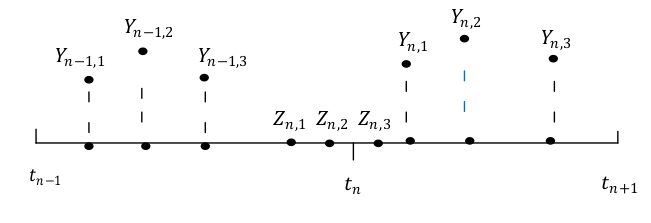
\includegraphics[width=12cm, height=4cm] {Interpolazioa}}
\caption{Interpolazioa.}
\label{fig:bost}
\end{figure}

\paragraph*{}($n-1$). urratseko informazioa erabiliz,
\begin{align*}
\left \{ \begin{array}{c}
Y_{n-1,i} =y_{n-1}+h \sum\limits_{j=1}^{s} a_{ij} f(Y_{n-1,j}),\\
y_n =y_{n-1}+h \sum\limits_{j=1}^{s} b_j f(Y_{n-1,j}),\\
\end{array} \right.
\ \Rightarrow \ \ 
Y_{n-1,i} &=y_n+h \sum\limits_{j=1}^{s} (a_{ij}-b_j) f(Y_{n-1,j}).
\end{align*}

Dagokion polinomio interpolatzailea,
\begin{equation*}
P(t)=  l_1(t) Y_{n-1,1}+\dots+l_s(t) Y_{n-1,s}+l_{s+1}(t) y_n
\end{equation*}
  
non $l_i(t)$ Lagrangiar polinomioa dugun,
\begin{equation*}
 l_i(t)=\prod_{l\neq i,l=1}^{s+1} \frac{(t-(t_{n-1}+hc_l))}{(c_i-c_l)}, \ \ c_{s+1}=1.
\end{equation*}

Eta beraz,
\begin{equation}
Y_{n,i} \approx Y_{n,i}^{[0]}= P(t_n+hc_i) = y_n+ h \sum\limits_{j=1}^{s} \lambda_{ij}f(Y_{n-1,j})
\end{equation}

\paragraph*{} Modu honetan s-ataletako IRK metodo bakoitzari dagokion $\lambda_{ij}$ koefiziente interpolatzaileak lortu daitezke. Polinomio interpolatzailearen bidezko hasieraketa ona izango da, emandako urratsa ez bada oso handia eta problema stiff ez denean. Era berean aipatu nahi genuke, atal askotako metodoetan (adibidez $s=16$)  interpolaziozko koefizienteen kalkuluan ezabapen arazoak,  doitasun handian lan egitea behartzen gaituela interpolaziozko hasieraketa ona izateko.  

\subsection{Algoritmoa.}

Formulazio berriari dagokion algoritmo orokorra,
%\begin{algorithm}[h]
% \BlankLine
%  $e_0=0$\;
%  \For{$n\leftarrow 0$ \KwTo ($endstep-1$)}
%  {
%   \BlankLine
%   Hasieratu  $Y_{n,i}^{[0]} \ \ , \ \ i=1,\dots,s $\;
%   \BlankLine
%   \While{ (konbergentzia lortu)}
%   {
%    \BlankLine 
%    $L_{n,i}=hb_if(Y_{n,i}) \ \ , \ \  i=1,\dots,s$\;
%    $Y_{n,i}=y_{n}+ \ \sum\limits_{j=1}^{s} \mu_{ij} L_{n,j}  \ \ , \ \  i=1,\dots,s$\;  
%   }
%   \BlankLine
%    $EL_{i}=hb_i \ f(Y_{n,i})-L_{n,i}, \ \ i=1,\dots,s$\;
%    $e_n=e_n+\sum\limits_{j=1}^{s}EL_{j}$\;
%    $\delta_{n}= \sum\limits_{i=1}^{s} L_{n,i}+e_n $\;
%    $y_{n+1}=y_{n}+ \delta_{n} $\;
%    $e_{n+1}=(y_{n}-y_{n+1})+\delta_n$\;
%   \BlankLine
% }
% \caption{Main Algorithm}
%\end{algorithm}

Eta puntu-finkoa erabiliz,

\begin{algorithm}[h]
 \BlankLine
  $e=0$\;
  \For{$n\leftarrow 0$ \KwTo ($endstep-1$)}
  {
   \BlankLine
   $k=0$\;
   Hasieratu  $Y_{n,i}^{[0]} \ \ , \ \ i=1,\dots,s $\;
   \BlankLine
   \While{ (konbergentzia lortu)}
   {
    \BlankLine 
    $k=k+1$\;
    $L_{n,i}^{[k]}=hb_if(Y_{n,i}^{[k-1]}) $\;
    $Y_{n.i}^{[k]}=y_{n} + \ \big(e+\sum\limits_{j=1}^{s} \mu_{ij} L_{n,j}^{[k]}\big)  $\;  
   }
   \BlankLine
    $EL_{i}=hb_i \ f(Y_{n,i})-L_{n,i}, \ \ i=1,\dots,s$\;
    $e=e+\sum\limits_{j=1}^{s}EL_{j}$\;
    $\delta_{n}= \sum\limits_{i=1}^{s} L_{n,i}^{[k]}+e $\;
    $y_{n+1}=y_{n}+ \delta_{n} $\;
    $e=(y_{n}-y_{n+1})+\delta_n$\;
   \BlankLine
 }
 \caption{IRK (puntu-finkoa).}
\end{algorithm}


\section{Esperimentuak.}


\subsection{Integrazio motak.}

Biribiltze erroreari dagokionez gure inplementazioa optimotik gertu dagoela erakutsi nahi dugu. Esperimentuetan lau integrazio mota egingo ditugu:

\begin{enumerate}

\item Koadruple doitasunezko ($128$-bit) integrazioa.

Zenbakizko integrazio hau soluzio zehatza kontsideratuko dugu eta errore globala kalkulatzeko erreferentziazko soluzioa izango da.

\item Integrazio ideala.

Koadruple doitasunezko integrazioa, ekuazio diferentzialaren eskuin aldeko funtzioaren ebaluazioa izan ezik. 
Ekuazio diferentziala double doitasunean ($64$-bit) definituko dela aurre baldintza harturik, integrazio ideala kontsideratuko dugu, hau da, hobetu ezin daitekeen integrazioa.    

\item Double doitasuna (batura konpensatu hobetua).

$64$-biteko koma higikorreko aritmetika eta \emph{batura konpensatua hobetua} erabiltzen duen inplementazioa, hau da,
atalen eguneraketan, ($\tilde{y}_n \oplus \tilde{e}_n$) (ekuazioa \ref{eq:eqbk}) espresioa erabilitako integrazioa.

\item Double doitasuna (batura konpensatu estandarra).

$64$-biteko koma higikorreko aritmetika eta \emph{batura konpensatu estandarra} erabiltzen duen inplementazioa (atalen eguneraketan $\tilde{e}_n$ gaia kontsideratzen ez duen integrazioa). 

\end{enumerate}

\subsection{Errore azterketa.}

Integrazio bakarra egin ordez, ausaz perturbatutako $P$ hasierako balio ezberdinetarako integrazioak exekutatu ditugu eta emaitza guzti hauen batazbestekoan oinarritu gara, biribiltze errorearen azterketa egokia egiteko.    

\subsubsection*{Adibidea.}

Ausazko perturbazioak kalkulatzeko funtzio bat definituta,
\begin{lstlisting} [language=Mathematica]
Pert[e0_,k_]:={e0*(k*RandomReal[{-1,1}])};
\end{lstlisting}

Perturbaziorik gabeko hasierako balioa $(u_0,e_0)$ eta $k$ perturbazio tamaina finkatuta, era honetan kalkulatuko dugu $(up_0,ep_0)$ perturbatutako hasierako balioa,
\begin{lstlisting} [language=Mathematica]
k = 2^35;
aux = Pert[e0, k];
up0 = N[u0] + aux;
aux2=up0-N[u0];
ep0=aux-aux2;
\end{lstlisting}


\subsubsection*{Notazioa.}  

$k$. integrazioan $N$ urrats eman baditugu, $t_i=t_0+i*h, \ i=1,\dots,N$ uneetarako lortuko dugu 
zenbakizko soluzioa,
\begin{equation*}
(q_i^{[k]},p_i^{[k]})\approx(q(t_i)^{[k]},p(t_i)^{[k]}), \ \ \ i=1,\dots,N.
\end{equation*}

\paragraph*{}Sistema Hamiltondarretan energia kontserbatzen da, energiaren definizioa hau izanik $H(q(t),p(t))=E(t)$,
\begin{equation*}
E_i^{[k]}=H(q_i^{[k]},p_i^{[k]})=konst, \ \ \ i=1,\dots,N.
\end{equation*}

\subsubsection*{Neurtzeko faktoreak.}

Energia eta kokapen erroreak honako faktoreen bidez neurtuko ditugu.

\begin{enumerate}

\item Energia errore globala.
%, \ \ i=1,\dots,N \ eta \ k=1,\dots,P.
\begin{align*}
\triangle E_i^{[k]} &=\frac{(E^{[k]}_i-E^{[k]}_0)}{E^{[k]}_0}, \ \ \ i=1,\dots,N \ eta \ k=1,\dots,P.\\
\bar{\triangle E_i} &=\frac{1}{P} \sum_{k=1}^{P} \triangle E_i^{[k]}, \ \  \sigma_i =\sqrt{\frac{1}{P} \sum_{k=1}^{P} (\triangle E_i^{[k]}-\bar{\triangle E_i})^2},\\
\bar{MaxE } &=\max_{i=1,\dots,N} |\bar{\triangle E_i}|.
\end{align*}  

\item Energia errore lokala.

$P$ integrazio guztietarako, bi urratsen arteko energia lokalaren batazbestekoa ($\mu$) eta desbiazio estarrada ($\sigma$).            
\begin{align*}
\blacktriangle E_i^{[k]} &=\frac{(E^{[k]}_i-E^{[k]}_{i-1})}{E^{[k]}_0},\ \ \ i=1,\dots,N \ eta \ k=1,\dots,P, \\
\bar{\mu} &= \frac{1}{N\cdot P} \bigg(\sum_{k=1}^{P} \sum_{i=1}^{N} {\blacktriangle E_i^{[k]}\bigg)}, \ \
\bar{\sigma} = \sqrt{\frac{1}{N\cdot P} \bigg(\sum_{k=1}^{P} \sum_{i=1}^{N} {(\blacktriangle E_i^{[k]}-\bar{\mu)}^2}\bigg)}          
\end{align*}
           
\item Kokapen errore globala.

Doitasun laukoitzean lortutako soluzioa, soluzio zehatza kontsideratuko dugu,           
\begin{equation*}
yexact^{[k]}_i=\hat{y}^{[k]}_i=(\hat{q}^{[k]}_i,\hat{p}^{[k]}_i).
\end{equation*}

eta $k.$ soluzioari dagokion kokapen errorea,          
\begin{align*}
Ge^{[k]}_i &=\|\hat{q}^{[k]}_i-q^{[k]}_i\|_2, \\
\bar{Ge_i}  &= (\frac{1}{P}\sum_{k=1}^{P} Ge^{[k]}_i) \ , \
                          \bar{MaxGe}=\max_{i=1,\dots,N} (\bar{Ge_i})
\end{align*}     
           
\item Puntu-finkoa lortutako urratsen batazbesteko portzentajea ($\bar{\triangle}0$).
           
$\triangle0^{[k]}$,  $k.$ integrazioan puntu-finkoa lortutako urratsen portzentaia izanik,           
\begin{equation*}
\bar{\triangle}0= \frac{1}{p}\sum_{k=1}^{P}\triangle0^{[k]}.
\end{equation*}
 
\item Kokapen errore estimazioa ($\bar{\mu Q_i}$ , $\bar{\sigma Q_i}$). 
            
Biribiltze errorearen estimazioaren gogoratuz, 
\begin{equation}
Est_i^{[k]}=\|(q_i^{[k]}+eq_{i}^{[k]})-(\tilde{\tilde{q}}_i^{[k]}+\tilde{\tilde{eq}}_{i}^{[k]})\|_2
\end{equation}
            
Errore estimazioaren kalitatea neurtzeko,
\begin{align} \label{eq:eq_Qi}
Q_i^{[k]} &=\log_{10} \bigg(\frac{Est^{[k]}_i}{Ge^{[k]}_i}\bigg),\\
\bar{\mu Q_i} &=\frac{1}{P}\sum_{k=1}^{p} Q_i^{[k]} \ , \ \ 
 \bar{\sigma Q_i}=\sqrt{\frac{1}{P}\sum_{k=1}^{P} (Q_i^{[k]}-\bar{\mu Q_i})^2}
\end{align}

\end{enumerate} 

\subsection{Integrazio parametroak.}

Hiru problemetarako esperimentuetan, integrazio parametroak bateratu ditugu. 

\begin{enumerate}

\item $s=6$ ataletako Gauss IRK metodoa aplikatu dugu.

\item Epe luzeko integrazioak aztertu ditugu.

\item Urratsa, trunkatze errorea biribiltze errorea baino txikiagoa izan dadin aukeratu dugu. 

\item Integrazio mota bakoitza $P=1.000$ perturbatutako hasierako balio ezberdinekin integratu dugu. Perturbazioen kalkulurako $k=2^35$ balioa finkatu dugu, hau da, $10^{-6}$ mailako perturbazioak aplikatu ditugu problema guztietarako.  

\item Kokapen errorearen estimazioaren kalkuluan, integrazio nagusian $rdigits1=0$ eta bigarren integrazioan $rdigits2=3$ balioak erabili ditugu.

\end{enumerate}


\subsection{Pendulu bikoitza ez-kaotikoa.}

Problema honetan zehazki erabilitako integrazio tartea eta urratsa hauek izan dira,
\begin{align*}
& t_0=0, \ \ t_{end}=2^{12}, \\
& h=2.^{-12}, \\
& sampling=2^7. 
\end{align*} 


\begin{table} [H]
\caption{Pendulu Bikoitza ez-kaotikoaren laburpena.}
\label{tab:2}       % Give a unique label
\begin{tabular}{c|c c c c c} 
 Integrazio Mota   &  $\bar{\triangle}0$  &  $\bar{MaxE}$ & $\bar{\mu}$  & $\bar{\sigma}$   & $\bar{MaxGe}$  \\
                           &   \%            &       &          &            &         \\
 \hline
                           &                 &         &       &           &          \\
 Koadruple                 &   $93.6$        &  $2e10^{-19}$  & $1e10^{-25}$  & $2e10^{-20}$  &      \\	    
 Ideala                    &   $98.3$        &  $7e10^{-16}$  & $6e10^{-19}$  & $2e10^{-17}$ &  $5e10^{-12}$\\
 Double                    &   $94.8$        &  $1e10^{-15}$  & $9e10^{-19}$  & $2e10^{-17}$ &  $7e10^{-12}$\\
\end{tabular}
\end{table}

\begin{figure}[!h]
\centering
\subfloat[Energi errorea.]{
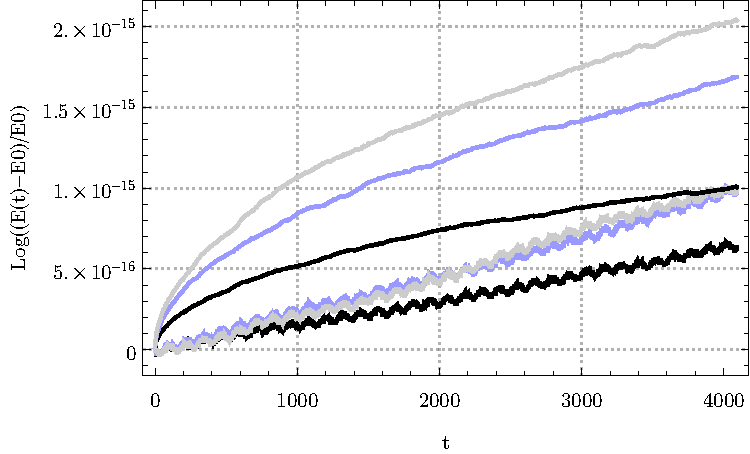
\includegraphics[width=.500\textwidth]{plot3a-2}
}
\subfloat[Kokapen errorea.]{
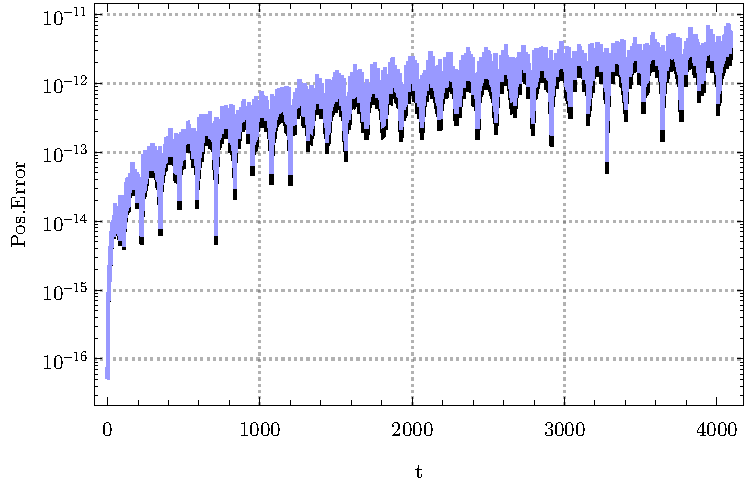
\includegraphics[width=.500\textwidth]{plot3b}
}
\caption[Pendulu-bikoitza: energi errorearen  eta kokapen errorearen eboluzioa.]
        {\small Pendulu-bikoitza ez-kaotikoa. Ezkerreko grafikoan,  energi errorearen batazbestekoa $\bar{\triangle E_i}$ eta desbiazio tipikoa $\sigma_i$ eboluzioa. Eskubiko grafikoan, kokapen errorearen eboluzioa $\bar{Ge_i}$. Integrazio ideala kolore beltzez, Double integrazioa (hobetua) kolore urdinez eta Double integrazioa (estandarra) gris kolorez.}
\label{fig:plot3}
\end{figure}        

\begin{figure}[!h]
\centering
\subfloat[Non-Chaotic: Ideal.]{
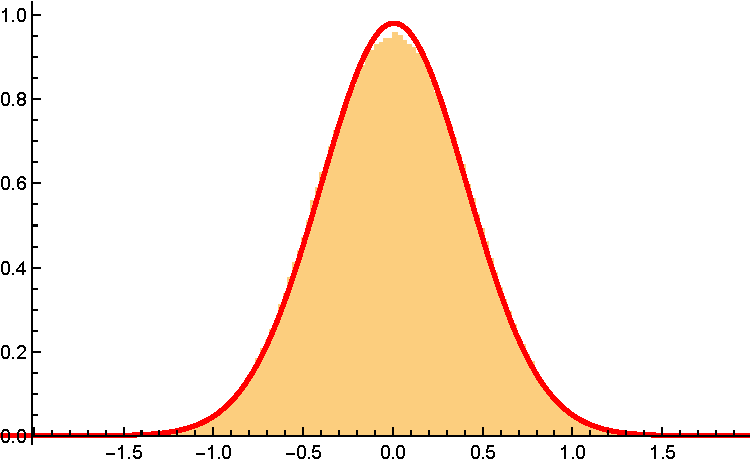
\includegraphics[width=.450\textwidth]{brouwer4a}
}
\subfloat[Non-Chaotic: rdigits=0.]{
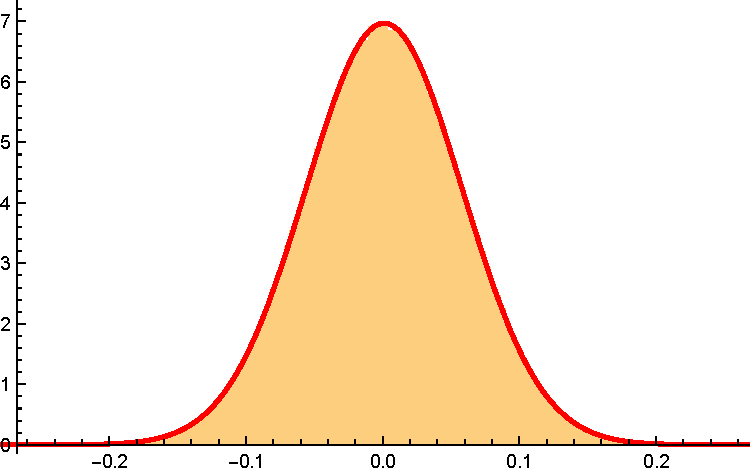
\includegraphics[width=.450\textwidth]{brouwer4b}
}
\caption{ \small Histogram of energy errors for Non-Chaotic case (a,b) and for Chaotic case (c,d).}
\label{fig:brouwer103}
\end{figure}


\begin{figure}[!h]
\centering
\subfloat[Non Chaotic: estimation]{
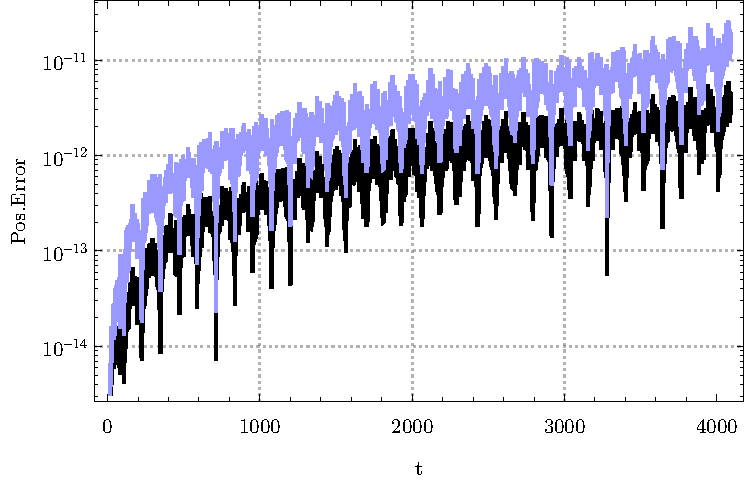
\includegraphics[width=.500\textwidth]{plot5a}
}
\subfloat[Non Chaotic: quality of estimation]{
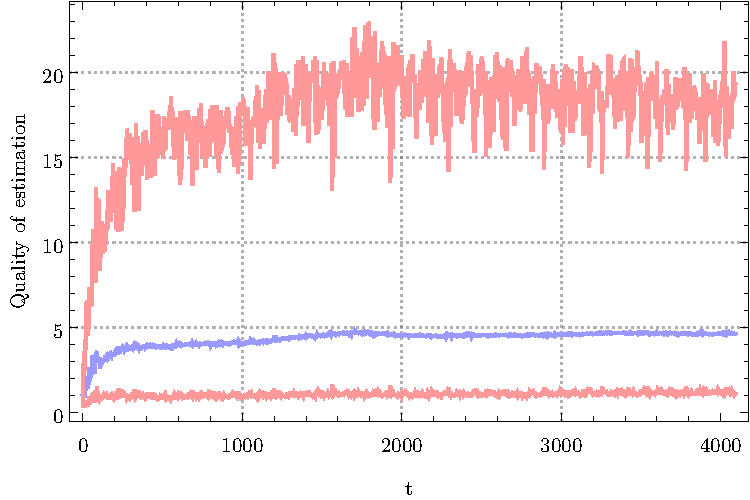
\includegraphics[width=.500\textwidth]{plot5b} 
}
\caption[Pendulu-bikoitza ez-kaotikoa: biribiltze errorearen estimazio.]

{\small Pendulu-bikoitza ez-kaotikoa: biribiltze errorearen estimazio. We compare evolution of our estimation error (blue) with evolution of global error (black). Estimation Quality. We show mean, $\bar{\mu Q_i}$ (blue) and  standard deviation, $\bar{\sigma Q_i}$ (red) of the quality according our definition of (\ref{eq:eq_Qi}).}
\label{fig:plotest}
\end{figure}

\clearpage
\subsection{Pendulu bikoitza kaotikoa.}

Problema honetan zehazki erabilitako integrazio tartea eta urratsa hauek izan dira,
\begin{align*}
& t_0=0, \ \ t_{end}=230, \\
& h=2.^{-12}, \\
& sampling=2^6. 
\end{align*} 


\begin{table} [h]
\caption{Summary of Chaotic case.}
\label{tab:3}       % Give a unique label
\begin{tabular}{c|c c c c c} 
 Arithmetic   &  $\bar{\triangle}0$  &  $\bar{MaxE}$ & $\bar{\mu}$  & $\bar{\sigma}$   & $\bar{MaxGe}$  \\
                           &   \%            &       &          &            &         \\
 \hline
                         &                 &         &       &             \\
 Quadruple prec          &   $93.6$        &  $2e10^{-19}$  & $7e10^{-22}$ & $1e10^{-20}$    &          \\	    
 Ideal Integrator        &   $98.3$        &  $3e10^{-16}$  & $1e10^{-18}$  & $9e10^{-18}$   & $0.18$    \\
 Double prec             &   $94.7$        &  $3e10^{-16}$  & $1e10^{-18}$  & $1e10^{-17}$   & $0.23$    \\
\end{tabular}
\end{table}


\subsubsection*{Energia eta kokapen erroreak.}


\subsubsection*{Brower legea.}

\begin{figure}[H]
\centering
\subfloat[Kaotikoa: Ideal.]{
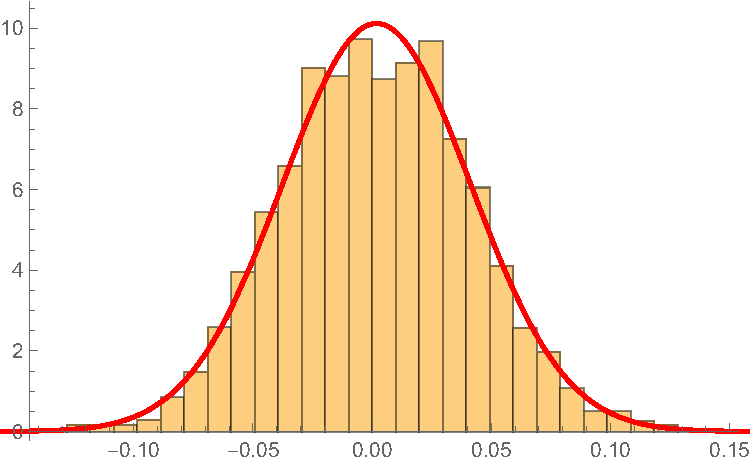
\includegraphics[width=.450\textwidth]{brouwer4c}
}
\subfloat[Kaotikoa: rdigits=0.]{
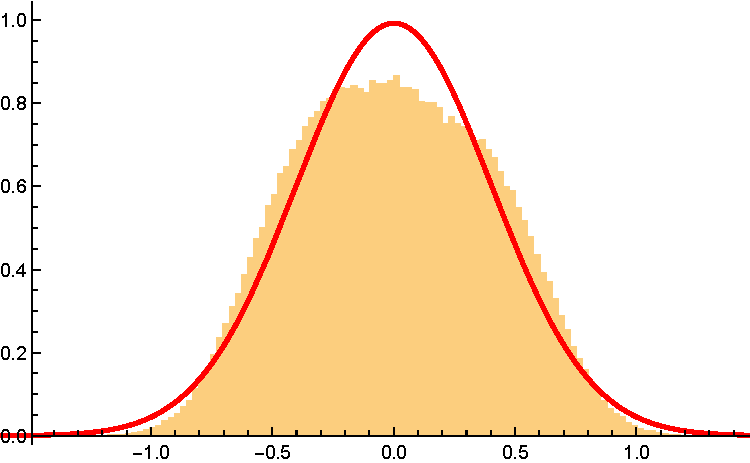
\includegraphics[width=.450\textwidth]{brouwer4d}
}
\caption{ \small Histogram of energy errors for Non-Chaotic case (a,b) and for Chaotic case (c,d).}
\label{fig:brouwer103}
\end{figure}

\subsubsection*{Errore estimazioa.}


\begin{figure}[h]
\centering
\subfloat[Non Chaotic: estimation]{
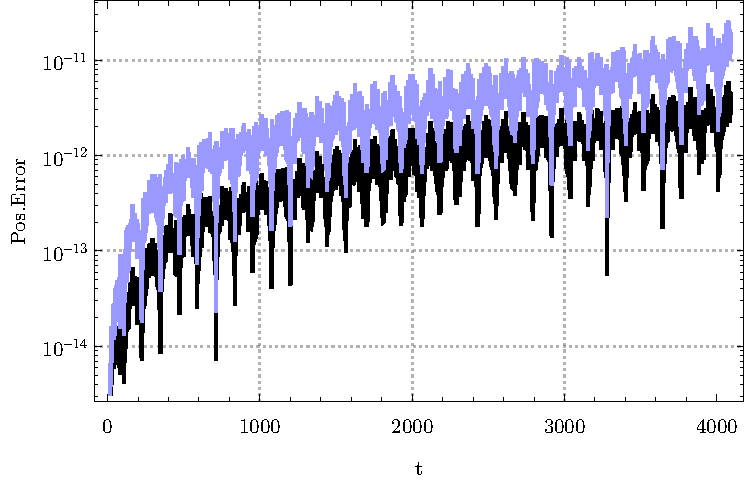
\includegraphics[width=.500\textwidth]{plot5a}
}
\subfloat[Non Chaotic: quality of estimation]{
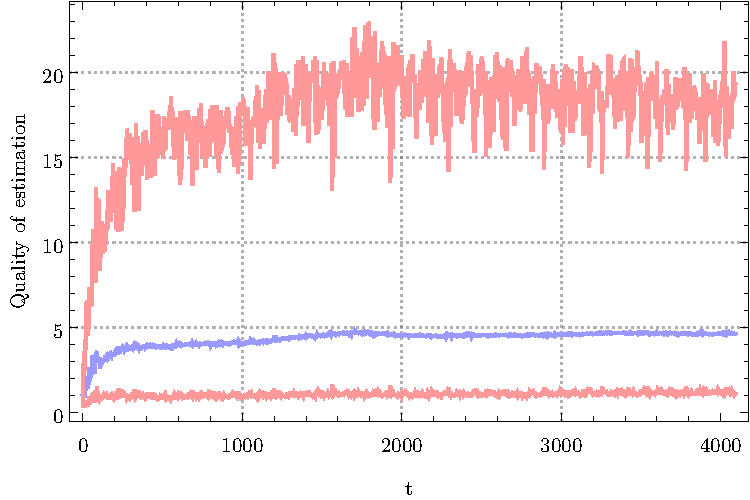
\includegraphics[width=.500\textwidth]{plot5b} 
}
\vskip\baselineskip
\subfloat[Chaotic: estimation]{
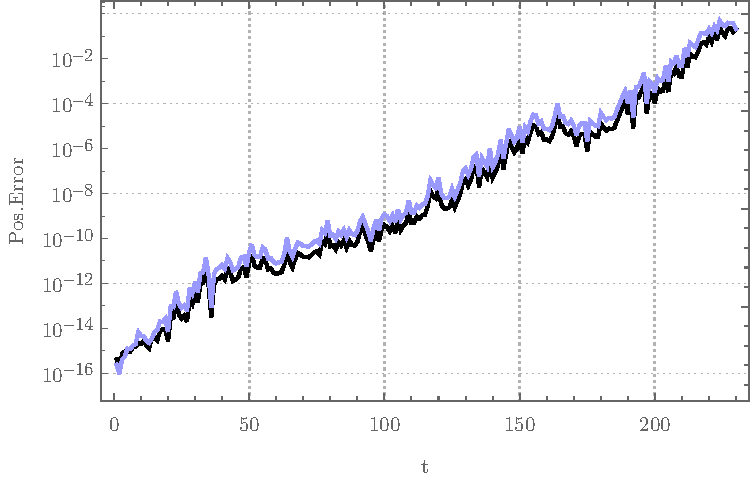
\includegraphics[width=.500\textwidth]{plot5c} 
}
\subfloat[Chaotic: quality of estimation]{
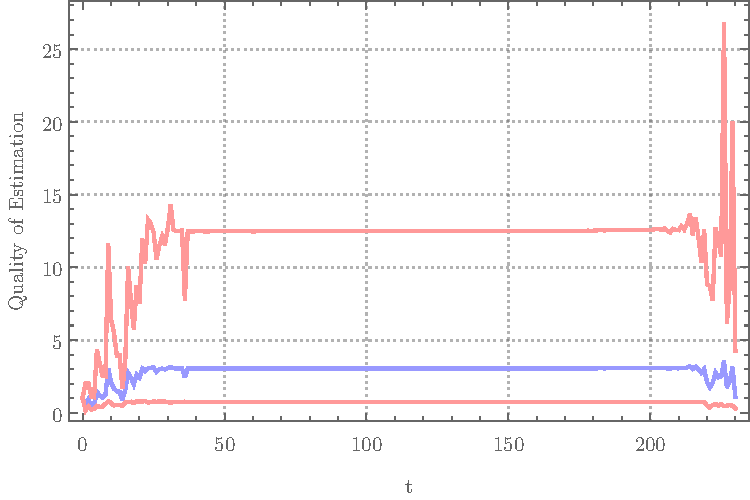
\includegraphics[width=.500\textwidth]{plot5d}
}

\caption[Pendulu-bikoitza: biribiltze errorearen estimazio.]{\small Estimation round-off error. We compare evolution of our estimation error (blue) with evolution of global error (black). Estimation Quality. We show mean (blue) and  standard deviation (red) of the quality according our definition of (\ref{eq:eq_Qi}).}
\label{fig:plotest}
\end{figure}

\clearpage
\subsection{N-Body problema.}


\begin{figure}[h]
\centering
\subfloat[Energy error.]{
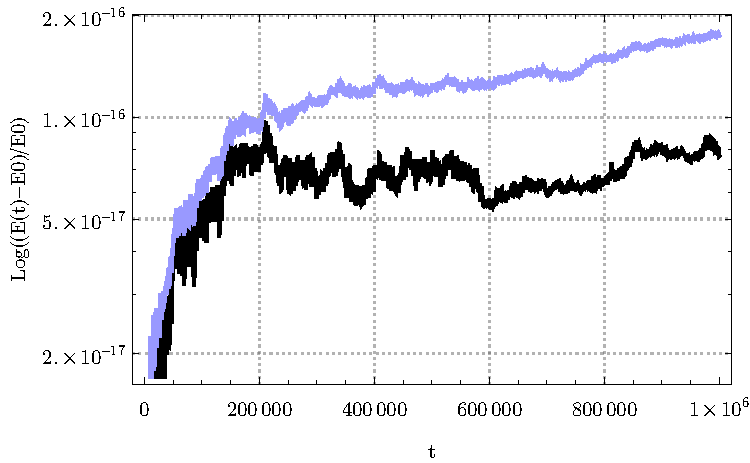
\includegraphics[width=.500\textwidth]{plot6a}
}
\subfloat[Global error.]{
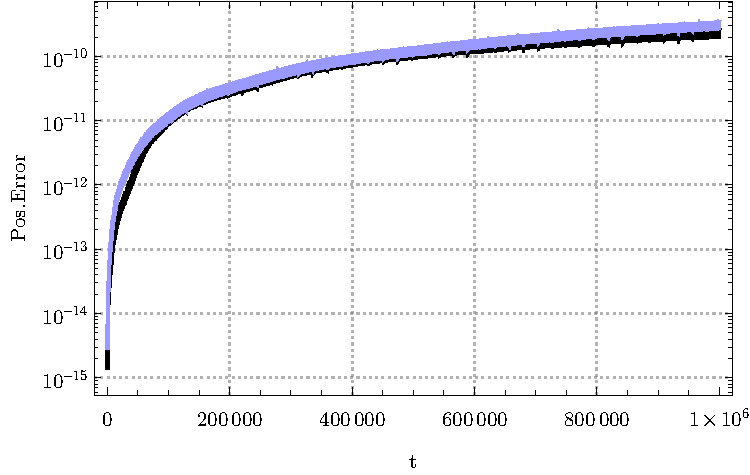
\includegraphics[width=.500\textwidth]{plot6b}
}
\caption[N-Body: energiaren errorearen eta errore globalaren eboluzioa.]{\small N-body: left figure mean energy error evolution $\bar{\triangle E_i}$ and right figure mean Global error evolution $\bar{Ge_i}$ of the 100 integrations for Ideal Integrator (black) and Double prec(blue).}
\label{fig:nbody1}
\end{figure}

\begin{figure}[h]
\centering
\subfloat[Estimation.]{
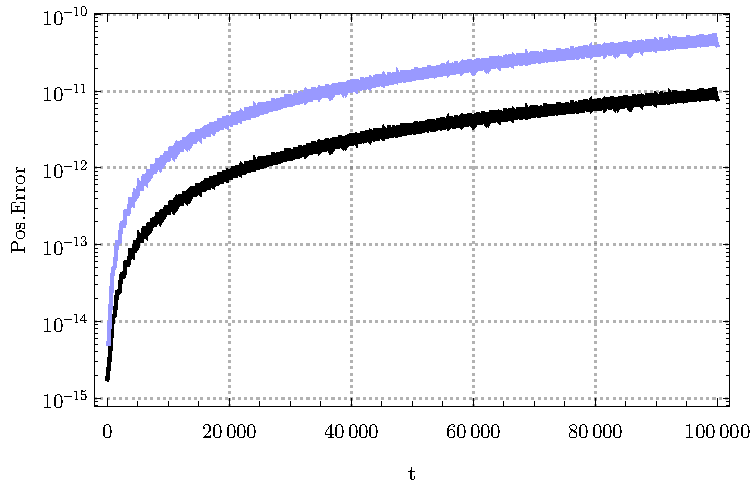
\includegraphics[width=.500\textwidth]{plot7a}
}
\subfloat[Quatlity.]{
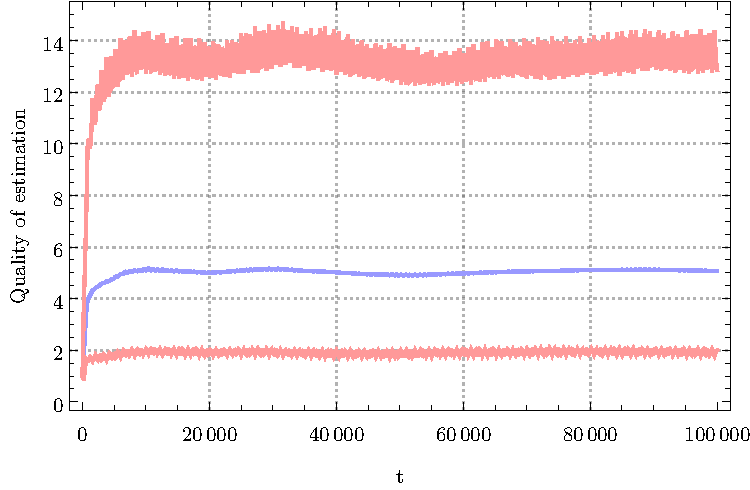
\includegraphics[width=.500\textwidth]{plot7b}
}
\caption[N-Body: birbiltze errorearen estimazioa.]{\small Left estimation round-off error, we compare evolution of our estimation error (blue) with evolution of global error (black). Right estimation Quality ,we show mean (blue) and  standard deviation (red) of the quality according our definition of (\ref{eq:eq_Qi}). We use rdigits1=0 and rdigits2=3.}
\label{fig:nbody2}
\end{figure}

\section{Laburpena.}

\chapter{IRK: Newtonen Iterazioa.}
\label{chap:IRK-NEW}
%\epigraph{The top 10 algorithms in Applied Mathematics: 1.Newton and quasi-Newton methods.}
%{\textit {Nick Higham (2016)}}

\section{Sarrera.}


Atal honetan, Newtonen iterazioan oinarritutako IRK metodoen inplementazio eraginkorra ikertuko dugu.
Problema zurruna denean, puntu-finkoaren iterazioa ez da eraginkorra eta Newtonen iterazioa aplikatu behar da. Gainera problema ez-zurruna izanik ere, Newtonen iterazioak interesgarriak izan daitezke; bereziki doitasun altuko (doitasun laukoitza) konputazioetan iterazio metodoaren konbergentzia ezaugarri onak direla-eta. 

Ikusiko dugunez, $d$-dimentsioko ekuazio diferentzialen sistema, Newtonen iterazioan oinarritutako $s$-ataletako IRK metodoaren bidez integratzeko, era honetako ekuazio-sistema lineala askatu behar da
\begin{equation}
\label{eq:syslin}
(I_d \otimes I_s- h \ A \otimes J) \in \mathbb{R}^{sd \times sd},
\end{equation} 
non $A \in \mathbb{R}^{s \times s}$ Runge-Kutta metodoaren koefizienteen den eta $J$ matrizea, ataletan ebaluatutako matrize Jacobiarraren  hurbilpen komuna den. Integrazioaren urrats bakoitzean, $sd \times sd$ tamainako ekuazio-sistema lineala askatu behar da.

Hainbat lanetan \cite{Butcher1976,Liniger1970,Bickart1977}, (\ref{eq:syslin}) matrizearen egitura berezia aprobetxatuz, ekuazio-sistema linealak modu eraginkorrean ebazteko proposamena egin zuten. Zehazki, ia blokeka diagonala den (\ref{eq:syslin})~matrizearen antzekoa era honetako $I_d-h \lambda_j J \in \mathbb{R}^{d \times d} \ (j=1,\dots,s)$ $s$-bloke duen matrizea, bloke bat $A$ matrizearen $\lambda_j$ balio propio  bakoitzeko. Normalean, ordena altuko IRK metodoaren koefizienteen $A$ matrizeak, $[s/2]$ balio propio konplexu pare ditu ($s$ bakoitia denean, balio propio erreal bat gehituta).

Gure ekarpenean, $sd$-dimentsioko (\ref{eq:syslin}) ekuazio-sistema, $(s+1)d$~dimentsioko sistema gisa 
berridatziko dugu, eta $d \times d$ tamainako $[s/2]+1$ matrizeren LU deskonposaketa (eta tamaina bereko matrize batzuen biderketa) kalkulatuz, askatuko dugu. Tamaina txikiko matrizeen LU deskonposaketa azkarra denez, konputazionalki eraginkorra izatea espero dugu. Inplementazioa, IRK metodo simetriko eta sinplektikoetarako garatu dugu. Dena den, bai IRK metodo ez-simetriko sinplektikoetarako, bai IRK metodo simetriko ez-sinplektikoetarako garatu daiteke.
 
Newtonen iterazio metodoaren bidez, $u\in \mathbb{R}^{n}$ eta $F: \mathbb{R}^n \ \longrightarrow {\mathbb{R}}^n$ emanik, $F(u)=0$ betetzen duen $u^{[*]}$ soluzioa aurkitu nahi dugu. Hasierako soluzioaren $u^{[0]}$ estimazioa  emanik,  Newtonen iterazio sinplifikatuaren definizioa \ref{alg:nssg}~algoritmoan ikus daiteke.

\begin{algorithm}[H]
  \BlankLine
  $ \text{Hasieratu} \ \ u^{[0]}   \quad \quad \quad \quad \quad \quad \quad \quad\quad \quad \quad \quad \quad \quad \quad \quad \quad    (64-bit)$\;
  $M=LU(J) \ \ \quad \quad \quad \quad \quad \quad \quad \quad\quad \quad \quad \quad \quad \quad \quad \quad \quad    (32-bit)$\;
  \For{ (k=1,2,\dots \text{konbergentzia lortu arte})}
  {
   \BlankLine
   $F^{[k]}=F(u^{[k-1]}) \  \quad \ \quad \quad \quad \quad \quad \quad \quad \quad \quad \quad \quad \quad \ \   (64-bit)$\;
   $\text{Askatu} \ \ M \ \Delta u^{[k]}=- F^{[k]} \ \quad \ \quad \quad \quad \quad \quad \quad \quad \quad \ \ \  (32-bit)$\;
   \BlankLine
   $u^{[k]}=u^{[k-1]}+\Delta u^{[k]}  \ \ \ \quad \quad \quad \quad\quad \quad \quad \quad \quad \quad \quad \ \     (64-bit)$\;
  }
 \caption{Newton sinplifikatua.}
 \label{alg:nssg}
\end{algorithm}
%
non $J \approx J(u^{[k]}) \in \mathbb{R}^{n \times n}$ matrize Jacobiarraren hurbilpena den,
\begin{equation*}
J(u^{[k]})=(J_{ij}(u^{[k]}))_{i,j}^n \ \text{non} \ J_{ij}(u^{[k]})=\partial F_i/\partial u_j (u^{[k]}), \ \ 1 \leq i,j \leq n. 
\end{equation*} 


Newton metodoaren eragiketa konplexuenak doitasun txikiagoan kalkula daitezke \cite{Baboulin20092526} eta honek, konputazionalki abantaila interesgarria suposatzen du. \ref{alg:nssg} algoritmoaren  eskuin aldean, inplementazioak erabilitako doitasuna $64$-biteko dela suposatuz, eragiketa bakoitzarentzat zein doitasun erabili beharko litzatekeen adierazi dugu; Jacobiarraren balioztapena eta aljebra linealeko eragiketak, doitasun arruntean ($32$-bit) kalkulatu daitezke. Horrela konputazio denbora azkartuko litzateke.

Newtonen iterazioan oinarritutako IRK metodoen azterketa, era honetan egituratu dugu. Lehenengo, (\ref{sec:7.2}) atalean, Newtonen iterazio estandarraren azalpenak eman ditugu eta notazioa finkatu dugu. (\ref{sec:7.3}) atalean, Newtonen iterazioen ekuazio-sistema modu eraginkorrean askatzeko teknika deskribatu dugu. Hurrengo, (\ref{sec:7.4})-(\ref{sec:7.5}) ataletan, Runge-Kutta metodoen formulazio berriarekin aplikatzeko zehaztasunak eman ditugu. (\ref{sec:7.6}) atalean, Newtonen iterazioan oinarritutako IRK metodoaren inplementazio berria aurkeztu dugu. Azkenik, (\ref{sec:7.7}) atalean, inplementazio berriarekin egindako zenbakizko esperimentuen emaitzak eman ditugu. 

\section{IRK-Newton estandarra.}
\label{sec:7.2}

Demagun honako hasierako baliodun problema,
\begin{equation}
\label{eq:hbp}
\dot{y}=f(t,y),\ \ \ y(t_0)=y_0, 
\end{equation}
non  $y_0 \in \mathbb{R}^{d}$  eta $f: \  {\mathbb{R}}^{d+1} \ \longrightarrow {\mathbb{R}}^d$ diren. 

Denbora diskretizazioa $t_0<t_1<t_2<\dots$ emanik, (\ref{eq:hbp}) hasierako baliodun problemaren $y(t)$ soluzioaren $y_n \approx y(t_n), (n=1,2,\dots)$ zenbakizko soluzioa, integrazio metodo bat aplikatuz lortuko dugu:
\begin{equation}
y_{n+1}=\Phi(y_n, t_n, t_{n+1}-t_n),
\end{equation}
non $\Phi:\mathbb{R}^{d+2} \rightarrow \mathbb{R}$ den.

S-ataletako IRK metodoaren kasuan,  $a_{ij}, b_i, \ \text{eta} \ c_i \ (1\leqslant i,j \leqslant s)$ koefizienteek definitzen dute $\Phi$ integrazio metodoa,
\begin{equation}  
\label{eq:irkn1}
\Phi(y,t,h)=y+h\sum^s_{i=1}{b_i \ f(t+c_ih,Y_{i})\ \ },\
\end{equation} 
%
non $c_i=\sum_{j=1}^{s} a_{ij}$ izan ohi den eta $Y_{i}$ atalak era honetan inplizituki  definitzen diren,
\begin{equation}
\label{eq:irkyi}
Y_{i}=y+\ h\ \sum^s_{j=1}{a_{ij}\ f(t+c_jh,Y_{j})}\ \ \ \ \ i=1 ,\dots, s.\
\end{equation} 

(\ref{eq:irkn1}) kalkulatu ahal izateko, $Y_{i} \in \mathbb{R}^d,\ i=1,\ldots,s$ ezezagunak lortu behar ditugu. Bakoitza $d$ dimentsiokoa denez, $sd$ tamainako ekuazio-sistema ez lineala adierazten du (\ref{eq:irkyi}) ekuazioak eta sistema hori askatzeko metodo iteratiboak erabil ditzakegu. Iterazio metodo sinpleena, puntu-finkoaren iterazioa da. Problema zurruna denean, puntu-finkoaren iterazioa ez da egokia eta orduan, Newtonen iterazioa aplikatu beharra dago. Problema ez-zurruna izanik ere, Newtonen iterazioak interesgarriak izan daitezke;
bereziki doitasun altuko (doitasun laukoitza) konputazioetan, doitasun ezberdinak nahasten \cite{Baboulin20092526} dituen teknikari esker (aljebra lienaleko eragiketak eta Jacobiarraren balioztapena doitasun txikiagoan kalkulatzea baitago).

Edozein kasutan, Newtonen iterazio bakoitzean, Jacobiarraren $s$ balioztapen eta $sd \times sd$ neurriko matrizearen LU deskonposaketa kalkulatu behar direnez, aldaera konputazionalki merkeagoak aplikatzen dira.

%Newton iterazio bakoitzean, $\partial f/ \partial y$ matrize jacobiarraren $s$ ebaluazio eta $sd \times sd$ tamaineko  matrizearen LU deskomposaketa kalkulatzea beharrezkoa da, eta beraz konputazionalki merkeagoak diren aldaerak erabili ohi dira.

\subsection*{Newton iterazioa.}

Newtonen iterazioan, (\ref{eq:irkyi}) ekuazio inplizituko $Y_i \ (i=1,\dots,s)$ atalentzako  $Y_i^{[k]}$ $k=1,2,\dots$ hurbilpenak kalkulatzeko algoritmoa, modu honetan defini daiteke,
\begin{align}
\label{eq:(1)Newton_iteration}
1) & \quad r_i^{[k]} := -Y_{i}^{[k-1]} + y + h \sum_{j=1}^{s}\, a_{ij}\, f(t + c_j h,Y_{j}^{[k-1]}), \quad  i=1 ,\ldots, s, \\
\label{eq:(2)Newton_iteration}
\begin{split}
2) & \quad \mathrm{Askatu \ } \Delta Y_{i}^{[k]},\\
& \quad \Delta Y_{i}^{[k]}  - h \sum_{j=1}^{s}\, a_{ij}\, J_j^{[k]} \Delta Y_{j}^{[k]} = r_i^{[k]} \quad  i=1 ,\ldots, s, \\
& \mbox{non} \quad  J_i^{[k]}=\frac{\partial f}{\partial y}(t + c_i h,Y_{i}^{[k-1]}) \quad \quad  i=1,\ldots, s, 
\end{split} \\
\label{eq:(3)Newton_iteration}
3)& \quad Y_i^{[k]} := Y_i^{[k-1]} + \Delta Y_i^{[k]}, \quad  i=1 ,\ldots, s,
\end{align}

Iterazio bakoitzeko,  $J_i^{[k]}$ Jacobiarraren $s$ ebaluazio eta $sd \times sd$ tamainako ekuazio-sistemaren LU deskonposaketa kalkulatu behar dugu. Eragiketa hauek konplexuak dira eta horregatik, Newton osoaren inplementazioa, konputazionalki garestia da. Aukera eraginkorragoen artean, bi aipatuko ditugu:

\begin{enumerate}
\item Newton sinplifikatuaren iterazioak aplikatzea. 
Aukera honetan, (\ref{eq:(2)Newton_iteration}) ekuazioaren $J_i^{[k]}$ Jacobiar matrizeak, $J_i^{[0]}=\frac{\partial f}{\partial y}(t+c_ih, Y_i^{[0]})$ matrizeekin ordezkatuko ditugu. Urrats bakoitzean, LU deskonposaketa behin bakarrik kalkulatu behar dugu.
\begin{equation*}
\Delta Y_{i}^{[k]}  - h \sum_{j=1}^{s}\, a_{ij}\, J_j^{[0]} \Delta Y_{j}^{[k]} = r_i^{[k]} \quad  i=1 ,\ldots, s.
\end{equation*}

Problema zurruna denean, atalen hasieraketa $Y i = y_n \ , \ i = 1, . . . , s$ erabili ohi da, eta orduan, $J_i^{[0]}=J:=\frac{\partial f}{\partial y}(y), \ i=1,\dots,s$ ordezkatuko dugu eta ekuazio-sistema lineala era honetan sinplifikatzen zaigu,
\begin{equation*}
(I_s \otimes I_d - h \ A \otimes J) \Delta Y^{[k]} = r^{[k]}.
\end{equation*} 

\item Jatorrizko Newtonen iterazioaren (\ref{eq:(2)Newton_iteration}) ekuazio-sistema, matrize honen,
\begin{equation}
\label{eq:irksys}
(I_s \otimes I_d - h \ A \otimes J)
\end{equation}
alderantzizkoarekin aurre-baldintzatuta, \cite{Saad2003} iterazio metodo  baten bidez ebaztea. Praktikan, (\ref{eq:(2)Newton_iteration}) ekuazio-sistemaren soluzioaren hurbilpen bat lortuko dugu, eta metodo hauek, Sasi-Newton (inexact Newton) izenarekin ezagutzen dira.    
\end{enumerate}

Aurreko bi aukeretan, era honetako ekuazio-sistemak askatu behar ditugu,
\begin{equation}
(I_d \otimes I_d - h \ A \otimes J) \ \Delta Y = r )
\end{equation} 
non $r \in R^{sd}$ den. Ekuazio-sistema $sd \times sd$ tamainako matrize osoaren LU deskonposaketa eginez ebatzi daiteke baina modu eraginkorragoan egiteko bideak aztertuko ditugu.

Modu estandarrean  \cite{Butcher1976,Liniger1970,Bickart1977} , $A$ matrizearen diagonalizazioa egiten da $\Lambda = S^{-1} A S=\mathrm{diag}(\lambda_1,\ldots,\lambda_s)$ eta ondorioz,
\begin{equation*}
I_s \otimes I_\dim  - h \, \Lambda \otimes J = (S^{-1} \otimes I_\dim) \left( I_s \otimes I_\dim  - h \, A \otimes J\right) (S \otimes I_\dim).
\end{equation*}
Beraz, ezker aldeko matrizearen LU deskonposaketa kalkulatuko da. Teknika honetan, $A$ matrizearen balio propio erreal (edo balio propio konplexu) bakoitzari dagokion $d \times d$ matrize errealen (edo konplexuen) LU deskonposaketak kalkulatu behar dira.

Beste autore batzuk \cite{Brugnano2014,Jay2009}, (\ref{eq:irksys}) ekuazio-sistema askatzeko, honako alderantzizko matrizea proposatzen dute:
\begin{equation}
I_d \otimes I_s -h \ \bar{A} \otimes J,
\end{equation}
non $\bar{A} \in \mathbb{R}^{s \times s}$ (LU deskonposaketa modu eraginkorragoan askatzeko aukeratua) aurre-baldintzatuta ebaztea proposatzen dute. 


\subsection*{Newton sinplifikatuaren iterazioa.}

Newton sinplifikatuaren iterazioan, $J_i^{[k]}$ Jacobiarrak,  $J_i^{[0]}=\partial f / \partial y \ (t+c_ih, Y_i^{[0]}) \ \ i=1,\cdots,s$ Jacobiarrez ordezkatzen dira eta orduan, askatu beharreko ekuazio-sistema honakoa da,
\begin{equation}
\label{eq:irks}
\Delta Y_{i}^{[k]}  - h \sum_{j=1}^{s}\, a_{ij}\, J_j^{[0]} \Delta Y_{j}^{[k]} = r_i^{[k]}, \quad  i=1 ,\ldots, s,
\end{equation}
non $\quad  J_i^{[0]}=\frac{\partial f}{\partial y}(t + c_i h,Y_{i}^{[0]}), \quad  i=1,\ldots,s \ $ den.

Lehen sinplifikazio honetan, integrazioaren urrats bakoitzeko,  $J_i^{[0]}$ Jacobiarraren s-ebaluazio eta $sd \times sd$ tamainako matrizearen LU deskonposaketa behin bakarrik kalkulatu behar dugu. Modu baliokidean, ekuazio lineala notazio matriziala erabiliz laburtu daiteke,
\begin{equation*}
\label{eq:805}
\left (I_s \otimes I_d - h  
\begin{bmatrix}
a_{11}  J_1^{[0]} & \dots & a_{1s}  J_s^{[0]} \\
a_{21}  J_1^{[0]} & \dots & a_{2s}  J_s^{[0]} \\
\vdots            & \ddots & \vdots \\
a_{s1}  J_1^{[0]} & \dots & a_{ss}  J_s^{[0]} \\ 
\end{bmatrix} \right) \Delta Y^{[k]} =r^{[k]}.
\end{equation*}

non,
\begin{equation*}
\label{eq:806}
Y^{[k]}=\begin{bmatrix}
Y_1^{[k]} \\
\vdots \\
Y_s^{[k]}
\end{bmatrix} \in \mathbb{R}^{sd}, \ \ \
r^{[k]}=\begin{bmatrix}
r_1^{[k]} \\
\vdots \\
r_s^{[k]}
\end{bmatrix} \in \mathbb{R}^{sd}.
\end{equation*}

%\begin{equation*}
%\label{eq:807}
%J_{is}(y)=\left(\partial f^i/\partial y^j (y)\right)_{i,j}^d=
%\begin{bmatrix}
%    \frac{\partial f^1}{\partial y^1} & \cdots & \frac{\partial f^1}{\partial y^d}\\    
%    \vdots & \ddots & \vdots \\    
%    \frac{\partial f^d}{\partial y^1} & \cdots & \frac{\partial f^d}{\partial y^d}\\    
%\end{bmatrix} \in \mathbb{R}^{d \times d},\ is=1,\cdots,s.
%\end{equation*}

\subsection*{Newton super-sinplifikatuaren iterazioa.}

Bigarren sinplifikazio bat aplika daiteke, $J_i^{[0]}=\partial f / \partial y \ (t+c_ih, Y_i^{[0]}), \ \  i=1,\dots,s \ $ matrizeak,  $J_i^{[0]} \approx J$ hurbilpen bakarrarekin ordezkatuz. Era honetako ekuazio-sistema lortuko dugu, 
\begin{equation}
\label{eq:irkss}
(I_s \otimes I_d - h \ A \otimes J) \Delta Y^{[k]} = r^{[k]}.
\end{equation}
non $I_s,I_d$ identitateak eta $A=(a_{ij})_{i,j}^s$ koefizienteen matrizeak diren.

Nahiz eta, $Y_i^{[0]}=y_n \ (i=1,\dots,s)$  ez den beste hasieraketa bat aplikatu, askotan gertatzen da (\ref{eq:irks}) sistema lineala, (\ref{eq:irkss}) sistemarekin ordezkatzea. Aukera egokia da ~\cite{Xie2009},  $J=  \frac{\partial f}{\partial y}(t+\bar c \, h,\bar y)$ aplikatzea, non $\bar c = \frac{1}{s} \sum_{i=1}^{s}c_i$ (metodo simetrikoetan $\bar c = \frac12$ da)  eta  $\bar y =  \frac{1}{s} \sum_{i=1}^{s}Y_i^{[0]}$ den. Maiz, $\partial f/\partial y$  konputazionalki merkeagoa den hurbilketa batez ordezkatzea, nahikoa izango da.      

Newtonen iterazioaren bertsio honi super-sinplifikatua deitu diogu. Iterazio bakoitzean $f$ funtzioaren $s$ ebaluazio eta $sd$ dimentsioko ekuazio-sistema lineala askatu behar da. $(I_s \otimes I_d - h \ A \otimes J)$ matrizea iterazio guztietarako berdina da,  bere LU deskonposaketa behin bakarrik egin behar da baina konputazionalki garestia da \cite{Butcher1976,Hairer1996}. Hau da aljebra linealari dagokion eragiketen konplexutasuna,
\begin{align*}
&\text{LU deskonposaketa}, \ \ 2s^3d^3/3+\mathcal{O}(d^2), \\
&\text{Back substitution}, \ \ 2s^2d^2+\mathcal{O}(d).
\end{align*}

Jarraian, Newton super-sinplifikatuaren inplementazioaren algoritmo orokorra laburtu dugu (\ref{alg:nss}~algoritmoa).

\subsection*{Algoritmoa.}

\begin{algorithm}[H]
 \BlankLine
  $\tilde{y}_0=fl(y_0)$\;
  $e_0=fl(y_0-\tilde{y}_0)$\;
  \For{$n\leftarrow 0$ \KwTo ($endstep-1$)}
  {
   \BlankLine
   $k=0$\;
   \text{Hasieratu} $Y_{n,i}^{[0]} \ \ , \ \ i=1,\dots,s $\;
   \BlankLine
   $J=\frac{\partial f}{\partial y}(t+h/2,y_n) $\; 
   $M=LU(I_s \otimes I_d - h \ A \otimes J)$\;
   \BlankLine
   \While{ (\text{not konbergentzia})}
   {
    \BlankLine 
    $k=k+1$\;
    $r_i^{[k]}=-Y_{n,i}^{[k-1]}+y_n+\big(e_n+h \sum\limits_{j=1}^{s} a_{ij} f(t+c_jh,Y_{n,j}^{[k-1]})\big) $\;
    \text{Askatu} $(M \Delta Y_n^{[k]}=r^{[k]})$\;
    $Y_n^{[k]}=Y_n^{[k-1]}+\Delta Y_n^{[k]}$\;
    $\text{konbergentzia} \leftarrow \text{GeratzeErizpidea}(Y_n^{[k]},Y_n^{[k-1]},\Delta_{min}) $\;
   }
   \BlankLine
   \If{($\exists j \ \text{non} \ \Delta_j^{[K]}\neq 0$)}
   {
    \If{$(NormalizeDistance(Y_n^{[k]},Y_n^{[k-1]})>1$}
     {$\text{fail convergence}$\;}
   }
   {$(\tilde y_{n+1},e_{n+1})\leftarrow \text{baturakonpensatua}(y_n,e_n,Y_n^{[k]})$\;}    
 }
 \caption{IRK (Newton super-sinplifikatua).}
 \label{alg:nss}
\end{algorithm}



\section{IRK-Newton eraginkorra.}
\label{sec:7.3}

\subsection{Ekuazio-sistema.}

Atal honetan, honako ekuazio-sistema lineala modu eraginkorrean askatzeko inplementazioa proposatuko dugu,
\begin{equation}
\label{eq:linsys}
(I_s \otimes I_d - h \ A \otimes J) \ \Delta Y = r,
\end{equation}
non $J \in \mathbb{R}^{d \times d}$  eta $r \in \mathbb{R}^{sd}$ diren.

$S$-ataletako IRK metodoa, Newton iterazioaren bidez $d$-dimentsioko ekuazio diferentzialen sistemari aplikatzeko, urrats bakoitzean $sd \times sd$ tamainako hainbat ekuazio-sistema (iterazio bakoitzeko bat) askatu behar dira. Atal honetan, jatorrizko $sd$-dimentsioko ekuazio-sistema, $(s+1)d$ dimentsioko ekuazio-sistema baliokide moduan berridatziko dugu. Ekuazio-sistema baliokide hau,  $d \times d$ tamainako $[s/2]+1$ matrize errealen LU deskonposaketa bidez askatuko dugu. Tamaina txikiko matrizeen LU deskonposaketa azkarra denez, konputazionalki eraginkorragoa izatea espero dugu.      

Gauss nodoetan oinarritutako Runge-Kutta kolokazio metodoak, sinplektikoak eta simetrikoak \cite{Sanz-Serna1992} dira. 
\begin{enumerate}
\item Sinplektikoa.

Runge-Kutta metodoa sinplektikoa izateko baldintza,
\begin{equation} 
\label{eq:sympl}
b_{i}a_{ij}+b_{j}a_{ji}-b_{i}b_{j}=0, \ \ 1 \leqslant i,j \leqslant s.
\end{equation} 
\item Simetrikoa.

Runge-Kutta metodoa simetrikoa izateko baldintza,
\begin{align}
\label{eq:simm}
\begin{split}
b_{s+1-i}=b_i, \ \ {c}_{s+1-i}=1-{c}_i,& \quad \ 1\leqslant i,j \leqslant s, \\
b_j={a}_{s+1-i,s+1-j}+a_{i,j},& \quad 1\leqslant i,j \leqslant s. 
\end{split}
\end{align} 
\end{enumerate}

Inplementazio eraginkorra garatzeko, goiko bi propietate hauetan oinarrituko gara.
S-ataletako IRK metodoaren (\ref{eq:irkn1}) formulazioa, modu baliokide honetan berridatzi daiteke,
\begin{equation}
\Phi(y,t,h):=y+z,
\end{equation}
non $Y_i \in \mathbb{R}^d$ atalak eta $z \in \mathbb{R}^d$ gehikuntza, inplizituki era honetan definitzen diren,
\begin{align}
&Y_{i}=y+\frac{z}{2}+ h\ \sum^s_{j=1}{\bar{a}_{ij}\ f(t+c_jh,Y_{j})}\ \ \ \ \ i=1 ,\dots, s,\\
&z=h \sum_{i=1}^{s} {b_i \ f(t+c_ih,Y_{i})},
\end{align} 
non
\begin{equation}
\bar{a}_{ij}=a_{ij}-\frac{b_j}{2}, \quad 1\leqslant i,j \leqslant s \ \ \text{den}.
\end{equation} 

Ekuazio inplizitua ebazteko Newtonen iterazio sinplifikatua aplikatzen badugu, $(s+1) \times d$ dimentsioko ekuazio-sistema askatu behar dugu,
\begin{align}
\label{eq:linsys2}
\begin{split}
(I_s \otimes I_d- h \ \bar{A} \otimes J) \ \Delta Y - \frac{1}{2}(e_s \otimes I_d) \ \Delta z =r,\\
(-h e_s^T B \otimes J) \ \Delta Y+  \Delta z=0,
\end{split}
\end{align}
non $e_s=(1,\dots,1)^T \in \mathbb{R}^{s}, \ \text{eta} \ \bar{A}=(\bar{a}_{ij})_{i,j=1}^s$ den. $(\Delta Y, \Delta z)$ (\ref{eq:linsys2}) ekuazio-sistemaren soluzioa bada, orduan $\Delta Y$ gure jatorrizko (\ref{eq:linsys}) ekuazio-sistemaren soluzioa da.

Ekuazio-sistemaren adierazpen matriziala lagungarria izan daiteke,
\begin{equation*}
\begin{bmatrix}
    &      &      &  & \ \ -I_d/2 \\
    &      &      &  & \ \ -I_d/2 \\
    &      &      &  & \ \      \\    
    &  & I_s \otimes I_d- h \ \bar{A} \otimes J & & \ \ \vdots \\
    &      &      &  & \ \      \\
    &      &      &  & \ \ \ \ -I_d/2    \\
-hb_1 J & -hb_2 J & \dots & -hb_s J &  I_d\\ 
\end{bmatrix}
\begin{bmatrix}
\Delta Y_1 \\
\Delta Y_2 \\
\vdots \\
\Delta Y_s \\
\Delta z\\
\end{bmatrix}=
\begin{bmatrix}
r_1 \\
r_2 \\
\vdots \\
r_s \\
0\\
\end{bmatrix}
\end{equation*} 

Aldi berean, koefiziente notazio berri hau finkatuta,
\begin{equation*}
\bar{c}_i=c_i-\frac{1}{2}, \quad \bar{a}_{ij}=a_{ij}-\frac{b_j}{2}, \quad 1\leqslant i,j \leqslant s,
\end{equation*}
dagokion propietate sinplektikoa (\ref{eq:sympl}) eta simetrikoa (\ref{eq:simm}) berridatziko ditugu,
\begin{enumerate}
\item {Sinplektikoa.}

Runge-Kutta metodoa sinplektikoa da,
\begin{equation}
\label{eq:eqlineala}
(B \bar{A}) \ \ \mbox{antisimetrikoa bada},
\end{equation}
non $\bar{A}=(\bar{a}_{ij})_{i,j=1}^s$ eta $B$, ($b_1,b_2,\dots,b_s$) balioen matrize diagonala diren.

\item {Simetrikoa.}

Runge-Kutta metodoa simetrikoa izango da, koefizienteek baldintza hauek betetzen dituztenean,
\begin{align}
\label{eq:simm2}
\begin{split}
b_{s+1-i}=b_i, \ \ \bar{c}_{s+1-i}=-\bar{c}_i,& \quad 1\leq i \leq s, \\
\bar{a}_{s+1-i,s+1-j}=-\bar{a}_{ij},& \quad 1\leq i,j \leq s. 
\end{split}
\end{align} 

\end{enumerate}

Inplementazio berrian, matrizeen dimentsioak zehazteko, parametro berri hauetan oinarrituko gara,
$m=[(s+1)/2]$, eta $s-m =[s/2]$. Metodoaren $s$-atalen kopurua bikoiti ala bakoiti izan, bi kasu bereiziko ditugu:
\begin{itemize}
\item $s$ bikoitia (Adibidea $s=6 \rightarrow m=3,\ s-m=3$).
\item $s$ bakoitia (Adibidea $s=7 \rightarrow m=4,\ s-m=3$).
\end{itemize}

\subsection{IRK metodo sinplektikoen garapena.}
\label{ss:733}

Lehenengo, IRK metodo sinplektikoak kontsideratuko ditugu. $(B \bar{A})$ antisimetrikoa bada, orduan $B^{1/2}\bar{A}B^{-1/2}$ antisimetrikoa da. Hori dela-eta, $\bar{A}$ diagonalizagarria da eta  balio propio irudikari puruak ditu. Beraz,  $Q, \ s \times s$ tamainako matrize ortogonala existitzen da,
\begin{align}
\label{eq:syb}
Q^{-1}\bar{A}Q=
\left(
\begin{matrix}
0 & D \\
-D^T & 0
\end{matrix}
\right)
\end{align}
non $D$,  balio erreal positiboen matrize diagonala eta $m \times (s-m)$ tamainakoa den. 

(\ref{eq:linsys2}) ekuazio-sistemari, aldagai aldaketa hau aplikatuz,
\begin{equation*}
 \Delta Y = (Q \otimes I_d) \ W,
\end{equation*}
%
honako ekuazio-sistema baliokidea lortuko dugu (garapenean (\ref{eq:syb}) erabili dugu),
\begin{equation}
\label{eq:linsys3}
\begin{split}
  \left(
  \begin{matrix}
    I_m \otimes I_\dim \ & \  -h \, D \otimes J  \\
    h \, D^T \otimes J \ & \ I_{s-m} \otimes I_\dim 
  \end{matrix}
\right) W -  \half\, (Q^{-1} e_s \otimes I_\dim) \, \Delta z &=  (Q^{-1} \otimes I_\dim )\, r, \\
- h \, (e_s^T  B Q \otimes J) \, W + \Delta z &= 0,
\end{split}
\end{equation}

(\ref{serans:B31}) eranskinean, ekuazio baliokideak lortzeko eman diren urratsen zehaztapenak eman ditugu. 

(\ref{eq:linsys3}) sistemaren  bloke bakanen egiturari esker, LU deskonposaketaren konputazioa, $d \times d$ tamainako matrizeen biderkaduren eta $[s/2]+1$ matrize errealen ($d \times d$) LU deskonposaketen bidez kalkulatuko dugu:
\begin{enumerate}
\item $I_\dim + h^2 \sigma_i^2 J^2 \in \mathbb{R}^{d \times d}, \quad i=1,\ldots,[s/2]$ matrizeen LU deskonposaketa,

non $\sigma_1,\ldots,\sigma_{[s/2]} \geq 0 , \ D$ matrizearen diagonaleko balioak diren.
\item Aurreko matrizeen espresiotik, lortutako $\dim \times \dim$ dimentsioko matrizearen LU deskonposaketa.
\end{enumerate} 


\subsection{IRK metodo simetriko sinplektikoen garapena.}
\label{ss:734}

Atal honetan, (\ref{eq:sympl}) propietate sinplektikoaz gain, (\ref{eq:simm}) simetria propietatea  ere betetzen duten IRK metodoak kontsideratuko ditugu. Lehenengo, garapenean erabiliko ditugun matrize laguntzaileak definituko ditugu.

\begin{enumerate}
\item P matrizea.

Kontsideratu $P=(P_1 \ P_2) \in \mathbb{R}^{s \times s}$ matrize ortogonala, non $P_1 \in \mathbb{R}^{s \times m}$ eta $P_2 \in \mathbb{R}^{s \times (s-m)}$ diren. Era honetan definituko dugu,  $x=(x_1,\dots,x_s)^T \in \mathbb{R}^s$, $P_1^Tx=(y_1,\dots,y_m)^T$, eta $P_2^Tx=(y_{m+1},\dots,y_s)^T$ non,
\begin{align*}
&y_i = \frac{\sqrt{2}}{2} (x_{s+1-i}+x_i), \ \ i=1,\dots,[s/2], \\
&y_i =\frac{\sqrt{2}}{2} (x_{s+1-i}-x_{i}), \ \ i=m+1,\dots,s, \\
&y_{m} = x_{m}, \ \ s \ \ \mbox{bakoitia bada}.
\end{align*}  

\item K matrizea.

Batetik, (\ref{eq:simm2}) simetria propietateak ,  $P_i^TB^{\frac{1}{2}}\bar{A}B^{-\frac{1}{2}}P_i=0, \ i=1,2$ dela eta bestetik, propietate sinplektikoak $B^{1/2}\bar{A}B^{-1/2}$ antisimetrikoa dela ziurtatzen dutenez, $\bar{A}$ matrizea honako matrizearen antzekoa dela ondorioztatu daiteke,
\begin{align}
P^TB^{\frac{1}{2}}\bar{A}B^{-\frac{1}{2}}P=
\left(
\begin{matrix}
0 & K \\
-K^T & 0
\end{matrix}
\right)
\end{align}
non $K=P_1^TB^{\frac{1}{2}}\bar{A}B^{-\frac{1}{2}}P_2 \ \in \mathbb{R}^{m \times (s-m)}$ den.

\item D matrizea.

$K=UDV^T$ balio singularren deskonposaketa izanik, non $U \in \mathbb{R}^{m \times m}$, eta $V \in \mathbb{R}^{(s-m) \times (s-m)}$ matrize ortonormalak diren eta $D \in \mathbb{R}^{m \times (s-m)}$, $K$ matrizearen balio singularren ($\sigma_1, \dots, \sigma_{s-m}$) matrize diagonala den,
\begin{align}
\label{eq:Dmat}
D=
\left(
\begin{matrix}
\sigma_1 & 0 & \dots & 0 \\
0 & \sigma_2 & \dots & 0 \\
0 & 0 & \dots & 0 \\
0 & 0 & \dots & \sigma_{s-m}
\end{matrix}
\right), \ \ \
D=
\left(
\begin{matrix}
\sigma_1 & 0 & \dots & 0 \\
0 & \sigma_2 & \dots & 0 \\
0 & 0 & \dots & 0 \\
0 & 0 & \dots & \sigma_{s-m} \\
0 & 0 & \dots & 0
\end{matrix}
\right).
\end{align}
s bikoitia bada, $D$ matrizea ezkerrekoa eta s bakoitia bada, $D$ matrizea eskuinekoa ($\sigma_m=0$) da. 

\item Q matrizea.

(\ref{eq:syb}) simetrikoa izategatik, berdintza hauek baieztatu daitezke,
\begin{align}
&Q=(Q_1 \ Q_2)=
B^{-1/2}(P_1 \ P_2)
\left(
\begin{matrix}
U & 0 \\
0 & V
\end{matrix}
\right)=
B^{-1/2} (P_1U \ P_2V), \\
&Q^{-1}=Q^TB.
\end{align}  

Matrizearen dimentsioak laburtuz, $Q=(Q_1 \ Q_2) \in \mathbb{R}^{s \times s}$, $Q_1 \in \mathbb{R}^{s \times m}$ eta $Q_2 \in \mathbb{R}^{s \times (s-m)}$ ditugu.

\end{enumerate}

(\ref{eq:linsys2}) ekuazio-sistemari, aldagai aldaketa hau aplikatuz,
\begin{equation}
\label{eq:DeltaYChVar}
 \Delta Y = (Q \otimes I_d) W= (Q_1 \otimes I_d) W'+ (Q_2 \otimes I_d) W'',
\end{equation}
\begin{align*}
\text{non}  \ \ W=\left(
\begin{matrix}
W^{'} \\
W^{''} 
\end{matrix}
\right),\ \ W^{'} \in \mathbb{R}^{m \times d}, \ \ W^{''} \in \mathbb{R}^{(s-m) \times d} \ \text{diren},
\end{align*}
%
eta metodoa simetrikoa denez, (\ref{eq:simm2}) baldintzetako lehenagatik , $e_s^TBP_2=0$ eta $\ e_s^TBQ_2=e_s^TBP_2V=0$~berdintasunak aplikatuz, honako ekuazio-sistema baliokidea lortuko dugu,
\begin{equation}
\label{eq:linsys4}
  \begin{split}
       W' -h \, (D \otimes J)\,  W'' - \half\, (Q_1^T B e_s \otimes I_\dim) \, \Delta z &= (Q_1^T B \otimes I_\dim )\, r, \\
    h \, (D^T \otimes J)\, W'  + W'' \phantom{+\half\, (Q_2^T B e_s \otimes I_\dim) \, \Delta z  }
    &= (Q_2^T B \otimes I_\dim )\, r,\\
-h \, (e_s^T  B  Q_1 \otimes J) \, W' + \Delta z &= 0.
  \end{split}
\end{equation}

(\ref{serans:B32}) eranskinean , ekuazioak lortzeko urratsen zehaztapenak eman ditugu.

\subsubsection*{Matrizearen egitura.}

 Aldagai aldaketarekin lortutako ekuazio-sistema, blokeka diagonala da eta hau aprobetxatuz, Newton iterazioaren inplementazio eraginkorra lortuko dugu. $S=6$ ataletako IRK metodoari dagokion ekuazio-sistemaren matrizearen egitura berezia hau da.    
\begin{equation*}
\label{eq:sysmat}
\begin{bmatrix}
 I_d        &             &                     & \multicolumn{1}{|c}{-h\sigma_1 J} &            &                  &\multicolumn{1}{|c}{-\frac{\alpha_1}{2} I_d}\\
            & I_d         &                     & \multicolumn{1}{|c}{}           & -h\sigma_2 J &                
 &\multicolumn{1}{|c}{-\frac{\alpha_2}{2} I_d}\\
            &             & I_d                 & \multicolumn{1}{|c}{}           &            & -h\sigma_3 J  
 &\multicolumn{1}{|c}{-\frac{\alpha_3}{2} I_d}\\\cline{1-7}    
h\sigma_1 J &             &                     & \multicolumn{1}{|c}{I_d}        &            &            
 &\multicolumn{1}{|c}{0}\\
            & h\sigma_2 J &                     & \multicolumn{1}{|c}{}           &  I_d       &             
 &\multicolumn{1}{|c}{0}\\
            &             &  h\sigma_3 J        & \multicolumn{1}{|c}{}           &            &  I_d        
 &\multicolumn{1}{|c}{0}\\\cline{1-7}
 -h\alpha_1 J       & -h\alpha_2 J              &  -h\alpha_3 J                    & \multicolumn{1}{|c}{$0$}        &  $0$       &  $0$         
 &\multicolumn{1}{|c}{ I_d}\\
\end{bmatrix}
\begin{bmatrix}
         \\
 W^{'} \\
    \\
\cline{1-1} \\
    \\
 W^{''}   \\
    \\
    \cline{1-1} \\
 \Delta z  \\
\end{bmatrix}=
\begin{bmatrix}
         \\
 R^{'} \\
    \\
\cline{1-1} \\
    \\
 R^{''}   \\
    \\
    \cline{1-1} \\
 0  \\
\end{bmatrix}
\end{equation*} 
non 
\begin{equation*}
\begin{bmatrix}
 R^{'}=(Q_1^{T}B^{1/2} \otimes I_d) \ r \\
 R^{''}=(Q_2^{T}B^{1/2} \otimes I_d) \ r
\end{bmatrix}, \ \
\left(
\begin{matrix}
\alpha_1 \\
\vdots \\
\alpha_m
\end{matrix}
\right)=Q_1^TB \ e_s.
\end{equation*}

Jarraian, ekuazio-sistemaren ezezagunak ($\Delta z,W^{'},W^{''}$) askatzeko aplikatuko ditugun espresioak laburtuko ditugu.

\paragraph*{$W^{''}$ kalkulatzeko ekuazioak.}

(\ref{eq:linsys4}) sistemaren  bigarren ekuaziotik $W^{''}$ askatu,
\begin{equation}
\label{eq:W''}
W^{''}= -h \ (D^T \otimes J) \ W^{'}+(Q_2^T B \otimes I_d) \ r.
\end{equation}

\paragraph*{$W^{'}$ kalkulatzeko ekuazioak.}

(\ref{eq:linsys4}) sistemako lehen ekuazioan $W^{''}$ ordezkatuz, honako ekuazio-sistema lortuko dugu,
\begin{align*}
(I_m \otimes I_d+ h^2DD^T \otimes J^2) \ W^{'}- \frac{1}{2}(Q_1^T B \ e_s \otimes I_d)\ \Delta z&=R, \\
- h \ (e_s^T B \ Q_1 \otimes J) \ W^{'} + \Delta z &=0,
\end{align*}
\begin{equation}
\label{eq:R}
\text{non} \ R=(Q_1^T B \otimes I_d) \ r + h \  ( D Q_2^T B \otimes J)\,  r \in \mathbb{R}^{md}.
\end{equation}

\paragraph*{}Goiko ekuazio-sistema honako notazioaren arabera,  
\begin{equation*}
R=\begin{bmatrix}
R_1 \\
\vdots \\
R_m
\end{bmatrix}, \ \ \
W^{'}=\begin{bmatrix}
W_1 \\
\vdots \\
W_m
\end{bmatrix}, 
\ \ R_i,W_i \in \mathbb{R}^d, \ \ i=1,\dots,m  
\end{equation*}

era honetan berridatziko dugu,
\begin{align}
\label{eq:linsys4a}
(I_d+h^2\sigma_i^2J^2) \ W_i- \frac{\alpha_i}{2}\ \Delta z &=R_i, \ i=1,\dots,m,\\
\label{eq:linsys4b}
-h \ J \sum\limits_{i=1}^{m} \alpha_i W_i+\Delta z &=0,
\end{align}
non,
\begin{align*}
\left(
\begin{matrix}
\alpha_1 \\
\vdots \\
\alpha_m
\end{matrix}
\right)=Q_1^TB \ e_s,
\end{align*}
eta $\sigma_1 \geqslant \cdots \geqslant \sigma_{s/2}, \ K$ matrizearen balio singularrak diren; $s$ bakoitia denean $\sigma_m=0$ dela gogoratu (\ref{eq:Dmat}). 

\paragraph*{$\Delta z$ kalkulatzeko ekuazioak.}

Aurreko (\ref{eq:linsys4a}) ekuaziotik, $W_i$ askatuz, 
\begin{equation*}
W_i=(I_d+h^2\sigma_i^2J^2)^{-1} (R_i+\frac{\alpha_i}{2} \ \Delta z),
\end{equation*}
%
eta (\ref{eq:linsys4b}) ekuazioan ordezkatuz, $\Delta z \in \mathbb{R}^d$ askatzeko ekuazioak lortuko ditugu,
\begin{equation}
\label{eq:linsys4c}
M\ \Delta z=h \ J\sum\limits_{i=1}^{m}\alpha_i (I_d+h^2\sigma_i^2J^2)^{-1}R_i,
\end{equation}
non
\begin{equation}M=I_d+ J \ \frac{h}{2}\ \sum\limits_{i=1}^{m} \alpha_i^2 (I_d+h^2 \sigma_i^2 J^2)^{-1} \in \mathbb{R}^{d \times d}.
\end{equation}

\paragraph*{Ezezagunak askatzeko laburpena.}

Sistemaren ezezagunak askatzeko ekuazioak eta ordena laburtuko dugu: lehenengo, $\Delta z \in \mathbb{R}^{d}$  (\ref{eq:linsys4c}) ekuaziotik askatuko dugu; bigarren,  $W^{'} \in \mathbb{R}^{md}$ (\ref{eq:linsys4a}) ekuaziotik askatuko dugu; hirugarren, $W^{''} \in \mathbb{R}^{(s-m)d}$ (\ref{eq:W''}) ekuaziotik askatuko dugu; eta azkenik, $\Delta Y$ (\ref{eq:DeltaYChVar}) ekuaziotik askatuko dugu.

\subsection{IRK Newton: konplexutasun analisia.}

$(I_s \otimes I_d - h \ A \otimes J) \Delta Y = r$ ekuazio sistema modu eraginkorrean askatzeko, inplementazio estandarraren eta gure inplementazioen konplexutasunak konparatuko ditugu.

\subsubsection*{Inplementazio estandarra.}

Butcher edota Hairer-en inplementazio estandarraren konputazioa bi modutan egin daiteke:

\begin{enumerate}
\item Zenbaki konplexuak.

$A$ matrizearen diagonalizazioak balio propio konplexuak ditu, 
\begin{equation*}
P^{-1}AP=\begin{bmatrix}
  \gamma_1 &                &          &                &           &                 \\
           & \bar{\gamma_1} &          &                &           &                 \\
           &                & \gamma_2 &                &           &                 \\
           &                &          & \bar{\gamma_2} &           &                 \\ 
           &                &          &                & \gamma_3   &                 \\
           &                &          &                &            & \bar{\gamma_3} \\  
\end{bmatrix},
\end{equation*}

eta ekuazio-sistema, zenbaki konplexuen aritmetika erabiliz ebatzi daiteke.
\begin{align*}
&(I-h \gamma_j J) \ X = b, \ \ j=1,\dots,3, \\
&(I-h \bar{\gamma}_j J) \ X = \bar{b}. 
\end{align*}

\item Zenbaki errealak.

Zenbaki konplexuekin ez bada lana egin nahi, zenbaki errealeko deskonposaketa baliokidea,
\begin{align*}
&\gamma_j=\alpha_j + i \ \beta_j,\\
&P^{-1}AP=\begin{bmatrix}
\alpha_{1} & -\beta_{1}   &  0            &  0            &  0           &    0       \\
\beta_{1}  & \alpha_{1}   & 0             &  0            &  0           &    0       \\
 0          & 0             & \alpha_{2}  & -\beta_{2}    &  0           &    0       \\
 0          & 0             & \beta_{2}   & \alpha_{2}    &  0           &    0       \\
 0          & 0             &  0          & 0             & \alpha_{3}  & -\beta_{3}  \\
 0          & 0             &  0          & 0             & \beta_{3}   & \alpha_{3}  \\
\end{bmatrix}
\end{align*}

\end{enumerate}

Hairer-en inplementazioan,
\begin{itemize}
\item $s$ bikoitia bada $\rightarrow$ $(2d \times 2d)$ tamainako $[s/2]$  LU deskonposaketa.
\item $s$ bakoitia bada $\rightarrow$ $(2d \times 2d)$ tamainako $(s+1)/2$  LU deskonposaketa.
\end{itemize}

\subsubsection*{Gure inplementazio berria.}

$\bar{A}$ matrizea, $\bar{A}=P^{-1}DP$ diagonalizatzen dugu eta $D$ matrizeak, irudikari puruak ditu,
\begin{equation*}
\bar{A}=Q^{-1}RQ, \ \,
R=\begin{bmatrix}
0           & -\gamma_{1}   &            &               &             &           \\
 \gamma_{1} & 0             &            &               &             &           \\
            &               & 0           & -\gamma_{2}  &             &           \\
            &               & \gamma_{2}  & 0              &           &           \\
            &               &             &                & 0            & -\gamma_{3} \\
            &               &             &                & \gamma_{3}   & 0            \\
\end{bmatrix}
\end{equation*}

Gure inplementazioan,
\begin{itemize}
\item $s$ bikoitia bada $\rightarrow$ $(d \times d)$ tamainako $[s/2]+1$  LU deskonposaketa.
\item $s$ bakoitia bada $\rightarrow$ $(d \times d)$ tamainako $(s+1)/2$  LU deskonposaketa.
\end{itemize}

\subsubsection*{Konplexutasun konparaketa}

Lehenengo eragiketa aljebraikoen konplexutasunak gogoratuko ditugu,
\begin{align*}
&\text{LU deskonposaketa}:  \ \ 2s^3d^3/3+\mathcal{O}(d^2), \\
&\text{Back substitution}:  \ \ 2s^2d^2+\mathcal{O}(d), \\
&\text{inv}: \ \ 2s^3d^3
\end{align*}

Bi inplementazioen konplexutasunen laburpena \ref{tab:Olu}~taulan ikus daiteke.
\begin{table}[h!]
\caption[LU deskonposaketak] 
{\small{}}
\label{tab:Olu}       
\centering
{%
\begin{tabular}{ l l l l l } 
 \hline
\\
                 &  \multicolumn{2}{c}{LU}  & \multicolumn{2}{c}{Back Substitution}  \\
 s               & Estandarra  & Berria     &  Estandarra  &              Berria     \\
\\
 \hline
\\
 $2m$            &   $\frac{8m}{3} d^3$                              &  $\frac{2}{3} (2m+1) d^3$ 
                 &   $4m (2d^2)$      &     $(6m+4)d^2$                                             \\
 \\
 $2m+1$          &   $\left(\frac{8m}{3} + \frac{2}{3}\right) d^3$   &  $\left(\frac{4m}{3}+\frac{2}{3}\right) d^3$
                 &   $(8m+2)d^2$      &     $(6m+4)d^2$\\  
 \\  
   \hline
 \end{tabular}}
\end{table}

\section{IRK-Newton estandarra (formulazio berria).}
\label{sec:7.4}

\ref{chap:IRK-PF}~atalean IRK puntu-finkoaren inplementazioan erabilitako  birformulazioa, IRK-Newton inplementazioan ere aplikatuko dugu. Horrela, IRK metodoa sinplektikoa izatea ziurtatzen dugu. IRK Newtonen iterazioaren inplementazioan ordea, $L_i$ ($i=1,\dots,s$) aldagai ezezagunak eta $Y_i$ ($i=1,\dots,s$) aldagai laguntzaileak kontsideratuko ditugu, biribiltze errorea gutxitzeko helburuarekin \cite{Olsson2000}.

IRK metodoaren formulazio estandarra (\ref{eq:irkn1}), era honetan berridatziko dugu,
\begin{equation}
\label{eq:PhiIRK2}
\Phi(y,t,h) :=y + \sum_{i=1}^s L_{i},
\end{equation}
%
non $L_{i} \in \R^d$, $i=1,\ldots,s$ inplizituki era honetan definitzen diren,
%
\begin{equation}
\label{eq:L}
 L_{i} = h \, b_i \, f(t+c_i h, y+ \sum_{j=1}^s \mu_{ij}\,L_{j}), \quad  i=1 ,\ldots, s, 
\end{equation}
%
eta
%
\begin{equation*} 
\mu_{ij}=a_{ij}/b_j,  \quad 1 \leq i,j \leq s.
\end{equation*}
%
\subsection*{Newton sinplifikatuaren iterazioa.}

Newtonen iterazioa formulazio berriarekin honakoa izango da; $L_i^{[0]}$ hasieratu eta  $k=1,2,\dots$ iterazioetarako, $L_i^{[k]}$ hurbilpenak era honetan kalkulatuko ditugu,
\begin{equation}
\label{eq:Newton_iteration2}
\begin{split}
1) 
   & \quad Y_i^{[k]} := y+\sum_{j=1}^{s}\, \mu_{ij}\, L_{j}^{[k-1]}, \quad  i=1 ,\ldots, s. \\
   & \quad g_i^{[k]} := -L_{i}^{[k-1]}  + h \, b_i\, f(t+c_i h,  Y_i^{[k]}), \quad  i=1 ,\ldots, s, \\   
2) & \quad \mathrm{Askatu \ } \Delta L_{i}^{[k]}  \\
   & \quad \Delta L_{i}^{[k]}  - h b_i J_i^{[k]} \sum_{j=1}^{s}\, \mu_{ij} \, \Delta L_{j}^{[k]}=g_i^{[k]}, \quad  i=1 ,\ldots, s,  \\
& \mbox{non} \quad  J_i^{[k]}=\frac{\partial f}{\partial y}(t + c_i h,Y_{i}^{[k-1]}),\quad \quad  i=1,\ldots, s,  \\
3) 
   & \quad   L^{[k]} := L^{[k-1]}  + \Delta L^{[k]}.
   \end{split}
\end{equation}

Newton sinplifikatuaren iterazioan, $J_i^{[k]}$ Jacobiarra $J_i^{[0]}=\partial f / \partial y \ (t+c_ih, Y_i^{[0]}) \ \ i=1,\cdots,s$ Jacobiarraz ordezkatzen da eta askatu beharreko ekuazio-sistema honakoa da,
\begin{equation*}
\Delta L_{i}^{[k]}  - h b_i J_i^{[0]} \sum_{j=1}^{s}\, \mu_{ij} \, \Delta L_{j}^{[k]}=g_i^{[k]}, \quad  i=1 ,\ldots, s.
\end{equation*}

Modu baliokidean, ekuazio lineala notazio matriziala erabiliz laburtu daiteke,
\begin{equation*}
\left (I_s \otimes I_d - h  
\begin{bmatrix}
b_1 \mu_{11} J_1^{[0]} & \dots & b_1 \mu_{1s} J_1^{[0]} \\
b_2 \mu_{21} J_2^{[0]} & \dots & b_2 \mu_{2s} J_2^{[0]} \\
\dots          & \ddots & \dots \\
b_s \mu_{s1} J_s^{[0]} & \dots & b_s \mu_{ss} J_s^{[0]} \\ 
\end{bmatrix} \right) \Delta L^{[k]} =g^{[k]},
\end{equation*}

non,
\begin{equation*}
L^{[k]}=\begin{bmatrix}
L_1^{[k]} \\
\vdots \\
L_s^{[k]}
\end{bmatrix} \in \mathbb{R}^{sd}, \ \ \
g^{[k]}=\begin{bmatrix}
g_1^{[k]} \\
\vdots \\
g_s^{[k]}
\end{bmatrix} \in \mathbb{R}^{sd},  
\end{equation*}

%\begin{equation*}
%\label{eq:907}
%J_{is}(y)=\left(\partial f^i/\partial y^j (y)\right)_{i,j}^d=
%\begin{bmatrix}
%    \frac{\partial f^1}{\partial y^1} & \cdots & \frac{\partial f^1}{\partial y^d}\\    
%    \vdots & \ddots & \vdots \\    
%    \frac{\partial f^d}{\partial y^1} & \cdots & \frac{\partial f^d}{\partial y^d}\\    
%\end{bmatrix} \in \mathbb{R}^{d \times d}, \ is=1,\cdots,s.
%\end{equation*}

\subsection*{Newton super-sinplifikatuaren iterazioa.}

Honako bigarren sinplifikazioarekin, $J_i^{[0]}=\partial f / \partial y \ (t+c_ih, Y_i^{[0]}), \ \  i=1,\dots,s$ matrizeak,  $J_i^{[0]} \approx J, \ i=0,\cdots,s$ hurbilpenaz ordezkatuz, ekuazio-sistema lineal hau lortuko dugu,
\begin{equation}
\label{eq:nsseq2}
(I_s \otimes I_d - h \ BAB^{-1} \otimes J) \ \Delta L = g. 
\end{equation}
non $I_d, I_s$ identitate matrizeak eta $B, \ (b_1,b_2,\dots,b_s)$ koefizienteen matrize diagonala diren.  

\subsection*{Algoritmoa.}

Formulazio berriari dagokion Newton super-sinplifikatuaren inplementazioa, (\ref{alg:nssli}) algoritmoan laburtu dugu.

\begin{algorithm}[H]
 \BlankLine
  $\tilde{y}_0=fl(y_0)$\;
  $e_0=fl(y_0-\tilde{y}_0)$\;
  \For{$n\leftarrow 0$ \KwTo ($endstep-1$)}
  {
   \BlankLine
   $k=0$\;
   $\text{Hasieratu} \ L_{n,i}^{[0]} \ , \ \ i=1,\dots,s $\;
   \BlankLine
   $J=\frac{\partial f}{\partial y}(y_n) $\; 
   $M=LU(I_s \otimes I_d - h \ BAB^{-1} \otimes J)$\;
   \BlankLine
   \While{ (\text{not konbergentzia})}
   {
    \BlankLine 
    $k=k+1$\;
    $Y_{n,i}^{[k]}=y_{n} + \ \big(e_n+\sum\limits_{j=1}^{s} \mu_{ij} L_{n,j}^{[k-1]}\big)  $\;
    $g_i^{[k]}=-L_{n,i}^{[k-1]}+h b_i f(t+c_ih,\ Y_{n,i}^{[k]})$\;
    \text{Askatu} $(M \Delta L_n^{[k]}=g^{[k]})$\;
    $L_n^{[k]}=L_n^{[k-1]}+\Delta L_n^{[k]}$\;
    $\text{konbergentzia} \leftarrow \text{GeratzeErizpidea}(L_n^{[k]},L_n^{[k-1]},\Delta_{min}) $\;
   }
   \BlankLine
   \If{($\exists j \ \text{non} \ \Delta_j^{[K]}\neq 0$)}
   {
    \If{$(NormalizeDistance(Y_n^{[k]},Y_n^{[k-1]})>1$}
    {$\text{fail convergence}$\;}
   }
   $\beta_{n}={e}_{n} + \sum\limits_{j=1}^{s}\Delta L_{n,j}^{[k]}$\;
   $(\tilde y_{n+1}, e_{n+1})\leftarrow \text{baturakonpensatua}(\tilde y_{n},\beta_{n},L_{n}^{[k-1]})$\;
 }
 \caption{IRK (Newton super-sinplifikatua).}
 \label{alg:nssli}
\end{algorithm}


\paragraph*{Interpolazio koefizienteak.} $L_{n,i}^{[0]}$ atalen hasieraketarentzat dagokien koefizienteak era honetan definituko ditugu: IRK puntu-finkoaren inplementazioan finkatu genituen (\ref{eq: interpLi}) interpolazio koefizienteetatik abiatuta  modu errazean definituko ditugu formulazio honi dagozkion interpolazio koefizienteak.
\begin{align}
\begin{split}
&\left \{ \begin{array}{c}
  Y_{n,i}^{[0]}=y_n+\sum_{j=1}^{s} \mu_{ij} L_{n,j}^{[0]} \\[.25cm]
  Y_{n,i}^{[0]}=y_n+\sum_{j=1}^{s} \nu_{ij} L_{n-1,j} \\
          \end{array} \right. 
\Rightarrow \ \ L_n^{{[0]}}=(Mu^{-1} Nu) L_{n-1},\\
\\
&\Rightarrow  \ \ (Mu^{-1} Nu)_{i,j}^{s}=\lambda_{ij}/a_{ij}.
\end{split}
\end{align}

\paragraph*{Geratze irizpidea.} Puntu-finkoaren iterazioan oinarritutako inplementazioarentzat definitutako geratze irizpide berdina (\ref{eq:not_stopping}) erabiliko dugu baina $L_{n,i}, \ i=1,\cdots,s$ aldagaiei aplikatuta.
\begin{equation*}
\Delta^{[k]}=(L_{n,1}^{[k]}-L_{n,1}^{[k-1]},\dots,L_{n,s}^{[k]}-L_{n,s}^{[k-1]}) \in \mathbb{F}^{sd},
\end{equation*}

Honako notazioa finkatuko dugu,
\begin{equation*}
\Delta_j^{[k]}, \ \text{non} \ \Delta^{[k]} \in \mathbb{F}^{sd}  \ (1\leqslant j \leqslant sd).
\end{equation*}
 Iterazioak  $k=1,2,\ldots$ jarraitzea , $ \Delta^{[k]} =0$ bete arte edo honako baldintza bi iterazio jarraietan bete arte,
\begin{equation}
\label{eq:not_stoppingLi}
\forall j \in \{1,\ldots,s d\},  \quad
\min \left(\{|\Delta_j^{[1]}|,\cdots ,|\Delta_j^{[k-1]}|\} \ /\{0\} \right) \leqslant |\Delta_j^{[k]}|.
\end{equation}


\paragraph*{Batura konpensatua.}

$\tilde{y}_{n+1}, e_{n+1} \in \mathbb{F}^d$, non $\tilde{y}_{n+1}+e_{n+1}\approx y(t_{n+1})$ era honetan kalkulatuko dugu:
\begin{enumerate}

\item $\Delta L^{[k]}$ gaiak gehitu.
\begin{equation*}
\delta_{n}={e}_{n} + \sum\limits_{j=1}^{s}\Delta L_{n,j}^{[k]}
\end{equation*}

\item Batura konpensatua.

Azkenik, batura konpensatua aplikatuko dugu,
\begin{equation}
\label{eq:bkLi2}
(\tilde y_{n+1}, e_{n+1}) = S_{s,d}(\tilde y_n, \delta_n, L_{n,1}^{[k-1]}, \dots,L_{n,s}^{[k-1]})
\end{equation}
 
\begin{algorithm}[H]
  \SetAlgoLined\DontPrintSemicolon
  \SetKwFunction{algo}{algo}\SetKwFunction{BaturaKonpensatua}{BaturaKonpensatua}
  \SetKwProg{myalg}{Algorithm}{}{}
  \SetKwProg{myproc}{Function}{}{}
  \myproc{\BaturaKonpensatua {$y_n$,\ $\delta_n$,\ $L_n^{[k-1]}$}}{
     \BlankLine
     $s_0=y_n$\;
     $ee=\delta_n$\;
     \For{$i\leftarrow 1$ \KwTo ($s$)}
      {
        $s_1=s_0$\;
        $inc= L_{n,i}^{[k-1]} +ee$\;
        $s_0=s_1+inc$\;
        $ee=(s_1 - s_0)+ inc$\;   
      }
     $y_{n+1}=s_0$\;
     $e_{n+1}=ee$\;    
    \KwRet ($y_{n+1}$,$e_{n+1}$) \;}
  \caption{BaturaKonpensatua $S_{s,d}(\tilde y_n, \delta_n, L_{n,1}^{[k-1]}, \dots,L_{n,s}^{[k-1]})$ funtzioaren inplementazioa da}
\end{algorithm} 

\end{enumerate}

\section{IRK-Newton eraginkorra (formulazio berria).}
\label{sec:7.5}

Formulazio berrian, modu eraginkorrean askatu behar dugun ekuazio-lineala honakoa da, 
\begin{equation}
\label{eq:linsysZG}
(I_s \otimes I_d - h \ BAB^{-1} \otimes J) \ \Delta L = g, 
\end{equation}
$J \in \mathbb{R}^{d \times d}$  eta ~$g \in \mathbb{R}^{s \times d}$ matrizeak izanik. 

(\ref{eq:linsysZG}) ekuazio-lineala  ebazteko, aurreko  \ref{ss:733}~atalean (\ref{eq:linsys}) moduko sistemak askatzeko deskribatutako teknika egokituko dugu. Jarraian, IRK metodo simetriko sinplektikoetarako (\ref{ss:734}~atala) garatutako teknika, formulazio berriko (\ref{eq:linsysZG}) sistema ebazteko nola aplikatu daitekeen deskribatuko dugu.

\subsection*{Formulazio estandarretik formulazio berrirako urratsa.}

Formulazio berriaren inplementazio eraginkorra, (\ref{ss:734}~atala) formulazio estandarrean emandako ekuazioak  moldatuz zehaztuko dugu.
Aurreko ataleko ekuazioetan, bi formulazioen aldagaien arteko erlazioak ordezkatuz,
\begin{align}
\label{eq:er1}
%&\Delta L =(B \otimes I_d) \ \Delta Y,\\
&\Delta Y = \Delta L \ (B \otimes I_d)^{-1} \\ 
\label{eq:er2}
&r=(B^{-1} \otimes I_d) \ g,
\end{align}

formulazio berrirako  ekuazio baliokideak lortuko ditugu.
\begin{enumerate}

\item Aldagai aldaketa.
Formulazio estandarraren (\ref{eq:DeltaYChVar}) aldagai aldaketari, (\ref{eq:er1}) ekuazioa ordezkatuz,
\begin{align}
\Delta L &=(B Q_1 \otimes I_d) \ W^{'}+(B Q_2 \otimes I_d) \ W^{''}.
\end{align}

\item $R\in \mathbb{R}^{md}$ matrizea.
Formulazio estandarreko $R$ matrizearen (\ref{eq:R}) ekuazioan, (\ref{eq:er2}) ekuazioa ordezkatuz,
\begin{align}
\begin{split}
R=&(Q_1^T \otimes I_d) \ g + h \ (D Q_2^T \otimes J) \ g,  \\
R=& Q_1^T \ g  + h D Q_2^T \ g \ J^T.
\end{split}
\end{align}

\item $W^{''}\in \mathbb{R}^{(s-m)d}$ matrizea.
Formulazio estandarraren $W^{''}$ matrizearen (\ref{eq:W''}) ekuazioan, (\ref{eq:er2}) ekuazioa ordezkatuz,
\begin{align}
W^{''}&= -h \ (D^T \otimes J) \ W^{'}+ (Q_2^T \otimes I_d) \ g.
\end{align}


\end{enumerate}


Formulazio berrian, IRK Newton sinplifikatuaren inplementazioaren urratsak hauek dira,
\begin{enumerate}

\item LU deskonposaketak.
    \begin{enumerate}
     \item $\mathbb{R}^{d \times d}$ matrizeen LU deskonposaketa,
         \begin{equation*}
         I_d+h^2 \sigma_i^2 J^2, \ i=1,\dots,[s/2].
         \end{equation*}
     \item $M \in \mathbb{R}^{d \times d}$ matrizea kalkulatu,
         \begin{equation*}
          M=I_d+J \ \frac{h}{2}\sum\limits_{i=1}^{m} \alpha_i^2 (I_d+h^2 \sigma_i^2 J^2)^{-1} \in \mathbb{R}^{d \times d}.
         \end{equation*}
      \item $M$ matrizearen LU deskonposaketa
         \begin{equation*}
          M \ \Delta z=h \ J\sum\limits_{i=1}^{m}\alpha_i (I_d+h^2\sigma_i^2J^2)^{-1}R_i.
         \end{equation*}
    \end{enumerate}


\item (\ref{eq:linsysZG}) ekuazio-sistemaren soluzioa ebatzi.
    \begin{itemize}
    %
    \item $R \in \mathbb{R}^{md}$ kalkulatu,
    \begin{equation*}
     R=(Q_1^T  \otimes I_\dim) \, g + h \,  ( D Q_2^T \otimes J)\, g.
    \end{equation*}
    %
    \item $d$ kalkulatu,
    \begin{equation*}
    d= h\, J \sum_{i=1}^{m} \alpha_i  (I_\dim +  h^2 \sigma_i^2 J^2)^{-1} R_i,
    \end{equation*}
    %
    \item $\Delta z \in \mathbb{R}^d$, ekuazio-sistematik askatu,
    \begin{equation*}
    M \ \Delta z=d.
    \end{equation*} 
    %
    \item $W_1, \dots, W_m \in \mathbb{R}^d$ kalkulatu,
    \begin{equation*}
    (I_\dim +  h^2 \sigma_i^2 J^2) \, W_i - \frac{\alpha_i}{2}\, J \, \Delta z = R_i, \quad i=1,\ldots,m.
    \end{equation*}
    %
    \item $W^{''} \in \R^{s\dim}$ kalkulatu,
    \begin{equation*}
     W^{''} = (-hD^T) \ W^{`} \ J^T+Q_2^T \ g.
    \end{equation*}
     %
     \item $\Delta L \in \mathbb{R}^{sd}$ kalkulatu,
     \begin{align*}
     \Delta L &=(B Q_1 \otimes I_d) W^{'}+(B Q_2 \otimes I_d) W^{''}, \\
     \end{align*}
    \end{itemize}

\end{enumerate}


IRK Newton sinlifikatuaren inplementazioa, \ref{alg:IRK-Newton-Li}~algoritmoan laburtu dugu. 

\begin{algorithm}[h!]
 \BlankLine
  $\tilde{y}_0=fl(y_0)$\;
  $e_0=fl(y_0-\tilde{y}_0)$\;
  \For{$n\leftarrow 0$ \KwTo ($endstep-1$)}
  {
   \BlankLine
   $k=0$\;
   \text{Hasieratu}  $L_{n,i}^{[0]} \ \ , \ \ i=1,\dots,s $\;
   \BlankLine
   $J=\frac{\partial f}{\partial y}(y_n) $\; 
   \BlankLine
   $ M=I_d+ \ J \ \frac{h}{2}\ \sum\limits_{i=1}^{m} \alpha_i^2 (I_d+h^2 \sigma_i^2 J^2)^{-1} $\;
   $ \mathrm{lum}=LU(M)$\;
   \BlankLine  
   \While{ (\text{not konbergentzia})}
   {
    \BlankLine 
    $k=k+1$\;
    $Y_{n,i}^{[k]}=y_{n} + \ \big(e_n+\sum\limits_{j=1}^{s} \mu_{ij} L_{n,j}^{[k-1]}\big)  $\;  
    \BlankLine
    $g_i^{[k]}= -L_{n,i}^{[k-1]}+ hb_i \ f(t+c_ih, Y_{n,i}^{[k]}) $\;
    \BlankLine
    $R=Q_1^T \ g  + (h D Q_2^T) \ g \ J^T $\;
    $d=h \ J \sum\limits_{i=1}^{m}\alpha_i (I_d+h^2\sigma_i^2J^2)^{-1}R_i$\;
    $\text{Solve}(\mathrm{lum} \ \Delta z = d)$\;
    \BlankLine 
    $W_i=(I_d+h^2\sigma_i^2J^2)^{-1} (R_i+\frac{\alpha_i}{2} \ \Delta z), \ i=1,\dots,m$\;
    \BlankLine
    $W^{``}= (-hD^T) \ W^{`} \ J^T+Q_2^T \ g$\;
    \BlankLine
    $\Delta L =B Q_1 \ W^{`}+B Q_2 \ W^{``} $\;
    $L_n^{[k]}=L_n^{[k-1]}+\Delta L_n^{[k]}$\;
    $\text{konbergentzia} \leftarrow \text{GeratzeErizpidea}(L_n^{[k]},L_n^{[k-1]},\Delta_{min}) $\;
   }
 \BlankLine
   \If{($\exists j \ \text{non} \ \Delta_j^{[K]}\neq 0$)}
   {
    \If{$(NormalizeDistance(Y_n^{[k]},Y_n^{[k-1]})>1$}
    {$\text{fail convergence}$\;}
   }
   $\delta_{n}={e}_{n} + \sum\limits_{j=1}^{s}\Delta L_{n,j}^{[k]}$\;
   $(\tilde y_{n+1}, e_{n+1})\leftarrow \text{baturakonpensatua}(\tilde y_{n},\delta_{n},L_{n}^{[k-1]})$\;
 }
 \caption{IRK (NSS-Eraginkorra).}
 \label{alg:IRK-Newton-Li}
\end{algorithm}


\clearpage


\section{IRK Newtonen iterazio mistoa.}
\label{sec:7.6}

\subsection{Sasi-Newton iterazioa.}

%Josebaren zuzenketa 22-05-2017
%Hurrengo  \ref{ss:ss762}~ataleko IRK metodoaren inplementazio berrirako, Newton iterazio metodoaren (\ref{eq:Newton_iteration2}) aldaera bat kontsideratuko dugu. Newtonen iterazio bakoitzaren ekuazio-sistema hau, 

Newton iterazio bakoitza, (\ref{eq:Newton_iteration2}) eskema jarraituz konputatzea da, eta egin beharretako bat ekuazio-sistema askatzea da. IRK metodoaren inplementazio berria ekuazio-sistema hori askatzeko metodoa aldatuko dugu, hau da, honako sistema,
\begin{equation}
\label{eq:linsysZ}
 \Delta L_{i}^{[k]}  - h b_i \ J_i \sum_{j=1}^{s}\, \mu_{ij} \, \Delta L_{j}^{[k]} = g_i^{[k]}, \quad  i=1 ,\ldots, s, 
\end{equation}
non
\begin{equation}
\label{eq:gk}
g_i^{[k]} = -L_{i}^{[k-1]}  + h \, b_i\, f\Big(t+c_i h,  y+\sum_{j=1}^{s}\, \mu_{ij}\, L_{j}^{[k-1]}\Big), \quad  i=1 ,\ldots, s, \\
\end{equation}
eta
\begin{equation*}
\Delta L^{[k]}= \left(
\begin{matrix}
\Delta L_1^{[k]}\\
\vdots\\
\Delta L_s^{[k]}
\end{matrix}
\right) \in \mathbb{R}^{sd}, \ \
g^{[k]}= \left(
\begin{matrix}
g_1^{[k]} \\
\vdots\\
g_s^{[k]}
\end{matrix}
\right) \in \mathbb{R}^{sd},
\end{equation*}
%
zehazki askatu beharrean, modu iteratiboan askatuko dugu. Horretarako,  \ref{alg:InexactNw}~algoritmoa aplikatuko dugu eta ~$\Delta L^{[k]} \in \mathbb{R}^{sd}$ soluzioaren  $ \Delta L_{i}^{[k,0]},  \Delta L_{i}^{[k,1]},  \Delta L_{i}^{[k,2]}, \ldots$ hurbilpenak kalkulatuko ditugu. 

\begin{algorithm}[H]
  $ \Delta L^{[k,0]} = (I_s \otimes I_d - h \ BAB^{-1} \otimes J)^{-1} \ g^{[k]}$\;
  \BlankLine
   \While{ $ \mathrm{GeratzeErizpidea}~(fl_{32}(\Delta L^{[k,0]}), \cdots,fl_{32}(\Delta L^{[k,l]}))  $ }
  {
   \BlankLine
   $l=l+1$\;
   $G_i^{[k,l]} = g_i^{[k]} - \Delta L_{i}^{[k,l-1]}  + h b_i \ J_i \sum_{j=1}^{s}\, \mu_{ij} \, \Delta L_{j}^{[k,l-1]},  \quad  i=1 ,\ldots, s$\;
   \BlankLine
   $\Delta L^{[k,l]}=\Delta L^{[k,l-1]}+ (I_s \otimes I_d - h \ BAB^{-1} \otimes J)^{-1} \ G^{[k,l]}$\;
  }
 \caption{Barne iterazioa.}
 \label{alg:InexactNw}
\end{algorithm}

non $fl_{32}(x), \ x \in \mathbb{R}$ zenbakitik gertuen dagoen $32$-biteko IEEE doitasun arrunteko balioa den.

IRK inplementazio berri honen \ref{alg:IRKstep}~algoritmoan, (\ref{eq:linsysZ})~ekuazio-sistema linealaren  $J_i$ Jacobiar matrizeen ebaluazioak, doitasun arrunta duten $Y_i$ atalekin kalkulatuko ditugu. Beraz, \ref{alg:InexactNw}~algoritmoaren iterazioen geratze irizpidea, $fl_{32}(\Delta L^{[k,l]})=fl_{32}(\Delta L^{[k,l-1]})$ doitasun arruntean betetzen dela aztertzea nahikoa izango dugu.  

\subsection{IRK Newton Mistoa}
\label{ss:ss762}

Zenbakizko soluzioa $y_n \approx y(t_n) \in \R^{d}, \ n=1,2,\dots$, bi bektoreen batura gisa, $ \ \tilde{y}_n+e_n \in \F^{d}$ lortuko dugu. Hasierako balioa $y_0 \in \R^{d}$, \ $\tilde{y}_0+e_0$ batura moduan adieraziko dugu, non $\tilde{y}_0=fl(y_0)$~ eta $e_0=fl(y_n-\tilde{y}_0)$ diren. 

Zehazki, $(\tilde{y}_{n+1}, e_{n+1})=\tilde{\Phi}(\tilde{y}_n, e_n, t_n, h)$  IRK metodoaren urrats berriaren zenbakizko soluzioa, bost faseetan kalkulatuko dugu:
 \begin{enumerate}
\item
$L^{[0]}=0 \in \R^{s\dim}$ atalak hasieratu, eta Newton super-sinplifikatuaren iterazioak aplikatu ((\ref{eq:Newton_iteration2}) iterazioaren ekuazio-sistema, (\ref{eq:nsseq2}) sistemarekin ordezkatuz), 
\[
L^{[1]}=L^{[0]} +\Delta L^{[1]}, \quad  L^{[2]}=L^{[1]} +\Delta L^{[2]} , \ldots
\]
geratze irizpidean, $ \fl_{32}(L^{[k]}) = \fl_{32}(L^{[k-1]})$ bete arte.

\item
$L^{[k]}$ berriari dagokion Jacobiarrak ebaluatu 
\begin{equation*}
J_i= \frac{\partial f}{\partial y}\left(t +c_i\,  h,  \ \tilde y+  \sum_{j=1}^{s}\, \mu_{ij}\, L_{j}^{[k]}\right), \quad i=1,\ldots,s.
\end{equation*}
%
\item
Lehen fasean lortutako $\Delta L^{[k]} \in \R^{s\dim}$ balioa,~(\ref{eq:linsysZ}) ekuazio-sistema linealaren $\Delta L^{[k]}$ soluzio zehatzaren $\Delta L^{[k,0]}$ hurbilpena kontsideratu eta 
\ref{alg:InexactNw}~algoritmoa aplikatu, $\Delta L^{[k]}$ soluzioaren $\Delta L^{[k,\ell]}$ hurbilpena (gutxienez doitasun arruntarekin) lortzeko.

\item 
$L^{[k]} = L^{[k-1]} + \Delta L^{[k,\ell]}$, eta $k=k+1$ eguneratu ondoren, Sasi-Newton iterazio bat aplikatuko dugu bigarren urratsean kalkulatutako $J_i$ Jacobiarren balioak erabiliz. Ekuazio-sistema linealaren (\ref{eq:linsysZ})-(\ref{eq:gk}), $ \ \Delta L^{[k]}$ soluzioaren  $\Delta L^{[k,\ell]}$ hurbilpenak (berriz ere doitasun arruntean)  \ref{alg:InexactNw}~algoritmoa aplikatuz kalkulatuko ditugu.

\item 
Azkenik, $(\tilde{y}_{n+1}, e_{n+1})=\tilde \Phi(\tilde{y}_n, e_n, t_n, h)$  urrats berriaren zenbakizko soluzioa kalkulatuko dugu,
\begin{equation*}
\tilde \Phi(\tilde{y}_n, e_n, t_n, h)=(\tilde y_n + e_n) + \sum_{i=1}^{s}(L_{n,i}^{[k-1]} + \Delta L_{n,i}^{[k,\ell]}).
\end{equation*}

Horretarako, Kahan-en batura konpensatua (\ref{alg:KahanBK}~algoritmoa) modu honetan aplikatuko dugu:
\begin{enumerate}
\item $\Delta L^{[k]}$ gaien batura (magnitude txikiko bektoreen batura).
\begin{equation*}
\delta_n :=  e_n + \sum_{i=1}^{s} \Delta L_{n,i}^{[k,\ell]})
\end{equation*}

\item Batura konpensatua.
\begin{equation*}
(\tilde y_{n+1},e_{n+1}) = S_{s,d}(\tilde y, \delta_n, L_{n,1}^{[k-1]}, \ldots, L_{n,s}^{[k-1]}).
\end{equation*}

\end{enumerate}

\end{enumerate}

 
Inplementazio honen hainbat zehaztasun azpimarratuko ditugu:
\begin{itemize}

\item Algoritmoaren era honetako sistema linealak $(I_s \otimes I_\dim  - h \, B A B^{-1} \otimes J )$, ~7.5.ataleko Newton inplementazio eraginkorrarekin  (\ref{alg:IRK-Newton-Li}~algoritmoa) askatuko ditugu.

\item $\mu_{i j} \in \F$ koefizienteek, zehazki (\ref{eq:simplektik2}) propietate sinplektikoa  eta simetria propietatea $\mu_{j, i} = \mu_{s+1-i,s+1-j}$  betetzen dituzte.

\item (\ref{eq:gk}) ekuazioaren $g_i^{[k]}$  ($i=1,\dots,s$) hondarren  konputaziorako, $y\in \R^\dim$~balioaren ordez, $\tilde y + e$ ($\tilde y, e \in \F^\dim$) espresioa erabili beharko litzateke. Hala ere, hori horrela egitearen eragina, oso txikia izango litzateke, eta azken Sasi-Newton iterazioan  bakarrik (4.fasea) kontutan hartzea erabaki dugu.  Gainera, azken Sasi-Newtonen iterazioan, (\ref{eq:gk}) ekuazioan $y$-ren ordez $\tilde{y}+e$ erabili beharrean, $J_i$ Jacobiarrak erabili ditugu honako hurbilketa egiteko:

\begin{gather*}
 h \, b_i\, f\left(t+c_i h, \ \tilde y + e +\sum_{j=1}^{s}\, \mu_{ij}\, L_{j}^{[k-1]}\right)  -L_{i}^{[k-1]} \approx \\
\left(h \, b_i\, f_i^{[k]} -L_{i}^{[k-1]} \right) + h\, b_i \, J_i \, e,
\end{gather*}
%
non $f_i^{[k]}=f\left(t+c_i h,  \tilde y +\sum_{j=1}^{s}\, \mu_{ij}\, L_{j}^{[k-1]}\right)$.

\end{itemize}

Inplementazioaren algoritmo osoa, \ref{alg:IRKstep}~algoritmoan laburtu dugu. 

 \begin{algorithm}[H]
  \BlankLine
    $L^{[0]} = 0$\;
    $J= \frac{\partial f}{\partial y}(t +h/2,\tilde y)$\;
    $M = I_\dim + J\, \frac{h}{2} \, \sum_{i=1}^m \alpha_i^2 (I_\dim +  h^2 \sigma_i^2 J^2)^{-1}$\;
    \BlankLine
    $\text{Compute the LU decomposition of M}$\;
    \BlankLine
    $\text{/************************** 1-Fasea **************************/}$\;
    \BlankLine
    $k=0$\;
   \While{ $\mathrm{ContFcn}(fl_{32}(L^{[0]}), \ldots, fl_{32}(L^{[k]}))$}
   {
    \BlankLine
    $k=k+1$\;        
    $Y_{i}^{[k]} = \tilde y+\sum_{j=1}^{s}\, \mu_{ij}\, L_{j}^{[k-1]}, \ i=1,\dots,s$\; 
    $f_{i}^{[k]} =  f\left(t+c_i h, Y_{i}^{[k]} \right), \ i=1,\dots,s$\;
    $g_i^{[k]} =h \, b_i\,f_i^{[k]} -L_i^{[k-1]}, \ i=1,\dots,s$\;
    $\Delta L^{[k]} =\left(I_s \otimes I_\dim  - h \, B A B^{-1} \otimes J \right)^{-1} g^{[k]}$\;
    $L^{[k]} = L^{[k-1]} + \Delta L^{[k]}$\;    
    %    $z^{[k]} = z^{[k-1]} + \Delta z^{[k]}$\;
            \BlankLine
   }
   \BlankLine
    $\text{/************************** 2-Fasea **************************/}$\;
   \BlankLine 
    $J_i= \frac{\partial f}{\partial y}\left(t + c_i h, \ \tilde y+\sum_{j=1}^{s}\, \mu_{ij}\, L_{j}^{[k]}\right), \ i=1,\dots,s$\;
   \BlankLine 
    $\text{/************************** 3-Fasea **************************/}$\;
   \BlankLine
    $ \ell=0$\;
    $\Delta L^{[k,0]} =  \Delta L^{[k]}$\;
    \While{$ \mathrm{ContFcn}(fl_{32}(\Delta L^{[k,0]}), \ldots, fl_{32}(\Delta L^{[k,\ell]}))$}
    {
    \BlankLine
    $\ell=\ell+1$\;
    $ G_i^{[k,\ell]} = g_i^{[k]} - \Delta L_{i}^{[k,\ell-1]}  + h b_i J_i \sum_{j=1}^{s}\, \mu_{ij} \, \Delta L_{j}^{[k,\ell-1]}, \ i=1,\dots,s$\;
    $\Delta L^{[k,\ell]} =\Delta L^{[k,\ell-1]} + \left(
         I_s \otimes I_\dim  - h \, B  A B^{-1} \otimes J \right)^{-1} 
          G^{[k,\ell]}$\;       
     \BlankLine
   }
    $L^{[k]} = L^{[k-1]} + \Delta L^{[k,\ell]}$\;    
    \BlankLine 
    $\text{/************************** 4-Fasea **************************/}$\;
    \BlankLine
    $k=k+1$\;
    $Y_{i}^{[k]} = \tilde y+ \sum_{j=1}^{s}\, \mu_{ij}\, L_{j}^{[k-1]}, \ i=1,\dots,s$\;
    $f_{i}^{[k]} =  f\left(t+c_i h, Y_{i}^{[k]} \right), \ i=1,\dots,s$\;
    $g_i^{[k]} = \left(h \, b_i\,f_i^{[k]} -L_i^{[k-1]} \right) + h \, b_i \, J_i \, e, \ i=1,\dots,s$\;
    \BlankLine
    $ \ell=0$\;
    $\Delta L^{[k,0]} =\left(
    I_s \otimes I_\dim  - h \, B A B^{-1} \otimes J \right)^{-1} g^{[k]}$\;
    \While{$ \mathrm{ContFcn}(fl_{32}(\Delta L^{[k,0]}), \ldots, \fl_{32}(\Delta L^{[k,\ell]}))$}
    {
    \BlankLine
    $\ell=\ell+1$\;
    $ G_i^{[k,\ell]} = g_i^{[k]} - \Delta L_{i}^{[k,\ell-1]}  + h b_i J_i \sum_{j=1}^{s}\, \mu_{ij} \, \Delta L_{j}^{[k,\ell-1]}, \ i=1,\dots,s$\;
    $\Delta L^{[k,\ell]} =\Delta L^{[k,\ell-1]} + \left(
         I_s \otimes I_\dim  - h \, B A B^{-1} \otimes J \right)^{-1} 
          G^{[k,\ell]}$\;       
    \BlankLine
    }
   \BlankLine 
    $\text{/************************** 5-Fasea **************************/}$\;
    \BlankLine
     $\delta = e + \sum_{i=1}^{s} \Delta L_i^{[k,\ell]}$\;
     $(\tilde y^*,e^*) = S_{s,d}(\tilde y, \delta, L_1^{[k-1]}, \ldots, L_s^{[k-1]})$\;
    \BlankLine
  \caption{IRK  Newtonen iterazio mistoa}
  \label{alg:IRKstep}
 \end{algorithm}

\clearpage

\section{Zenbakizko esperimentuak.}
\label{sec:7.7}

\label{s:ne}

Newton iterazioan oinarritutako $6$-ataletako Gauss kolokazio metodoaren inplementazioarekin egindako zenbakizko esperimentuak azalduko ditugu. Esperimentu hauen konputaziorako, $64$-biteko doitasuneko IEEE koma-higikorreko aritmetika erabili dugu.

\subsection{Problemak}

\subsubsection*{Pendulu bikiotz zurruna}

Pendulu bikoitz zurrunaren problemaren Hamiltondarra eta parametroak, \ref{ss:322}~atalean definitu ditugu. $k$ parametroak malgukiaren zurruntasun maila finkatzen du: $k=0$ balioarentzat, problema ez da zurruna eta problemaren zurruntasuna, $k$ balioarekin batera handitzen da. 

Hasierako balioak, era honetan aukeratu ditugu: $k=0$ problema ez zurrunarentzat, \cite{Dumitru} artikulutik izaera ez-kaotikoa duen hasierako balioa hartu dugu: $q(0)=(1.1, -1.1)$ eta $p(0)=(2.7746,2.7746)$. $k\neq 0$ problemen hasierako balioak,
\begin{equation*}
q(0)=\left(1.1, \frac{-1.1}{\sqrt{1+100k}}\right), \ \ 
p(0)=(2.7746,2.7746),
\end{equation*}
espresioen bidez finkatu  ditugu, horrela sistemaren energia $k \rightarrow \infty$ handitzen den heinean, bornatua dago.

Integrazio guztiak, $h=2^{-7}$ urrats luzera erabiliz egin ditugu; problema ez zurrunarentzat ($k=0$) trunkatze errorea biribiltze errorea baino txikiago izan dadin aukeratu dugu. Trunkatze errorea, biribiltze errorea baino handiagoa izango da $k>0$ zurruntasun balio handietarako. $T_{end}=2^{12}$ segundoko integrazioak egin ditugu eta zenbakizko soluzioa, $m=2^{10}$ urratsero itzuli dugu. 

\subsection{Biribiltze errorearen azterketa.}

Lehenengo, Newtonen iterazioan oinarritutako IRK inplementazio berriaren biribiltze errorearen hedapena egokia dela aztertuko dugu. Aurreko artikuluan \cite{Antonana2017},  biribiltze errorearen hedapena gutxitzeko ahalegin berezia eginez,  puntu-finkoaren iterazioan oinarritutako IRK inplementazioa proposatu genuen. Bi inplementazioen, 6-ataleko Gauss kolokazio metodoaren  biribiltze erroreak konparatuko ditugu.

Pendulu bikoitzaren $k$ parametroaren hiru balioetarako, energia errorearen azterketa zehatza egin dugu: $k=0$ , non biribiltze errorea trunkatze erroreari nagusitzen zaion; $k=2^{10}$, non bi erroreak tamaina berekoak diren; eta $k=2^{12}$, non trunkatze errorea birbiltze erroreari nagusitzen zaion. Biribiltze errorearen konparaketa sendoago izan dadin (\cite{Hairer2008}~lanean bezala), azterketa estatistikoa egin dugu. Problema bakoitzarentzat, hasierako balioak $\mathcal{O}(10^{-6})$ errore tamainako ausaz perturbatutako $P=1000$ integrazio konputatu ditugu. 

\ref{fig:plot3}~irudian, zenbakizko integrazioek gure inplementazio berriaren biribiltze errorearen propagazio ona erakusten dute. Alde batetik, $k=0$ eta $k=2^{10}$ balioetarako, puntu-finkoaren iterazioan oinarritutako inplementazioak energiaren grapenaren batezbestekoak, drift lineala agertzen du eta Newton iterazioan oinarritutako inplementazioak, ordea ez du energia driftarik agertzen. Beste alde batetik, bi inplementazioetan, energiaren desbideratze estandarrak antzekoak dira eta $t^{1/2}$ espresioaren proportzionalak dira.   

\begin{figure}[h!]
\centering
\begin{tabular}{c c}
\subfloat[$k=0$ energia errorrearen batezbestekoa ]
{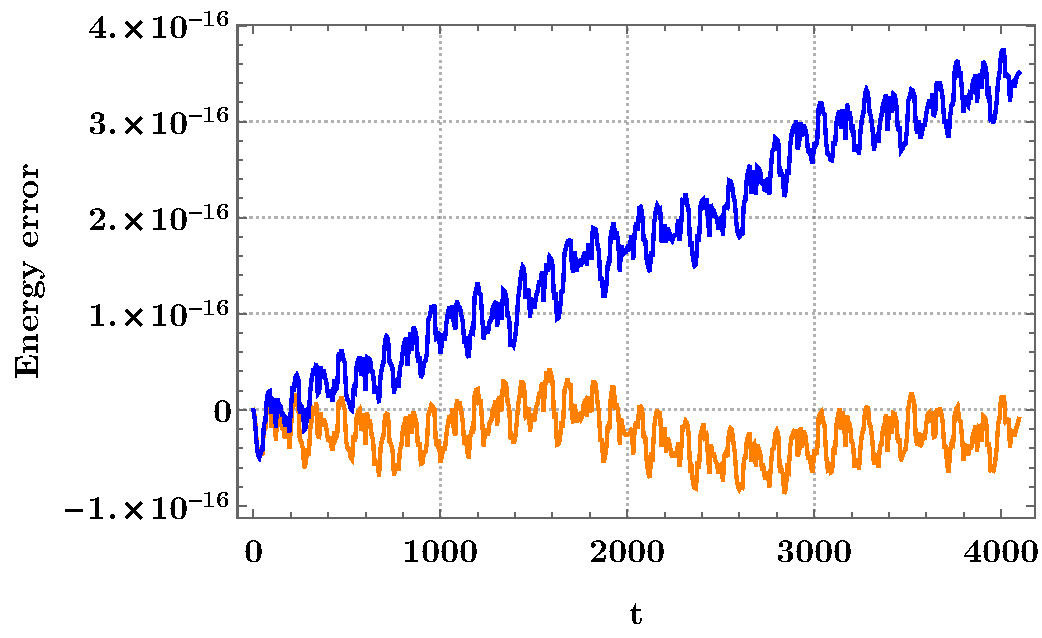
\includegraphics[width=.4\textwidth]{Fig2N}}
&
\subfloat[$k=0$ energia errorearen desbideratze estandarra]
{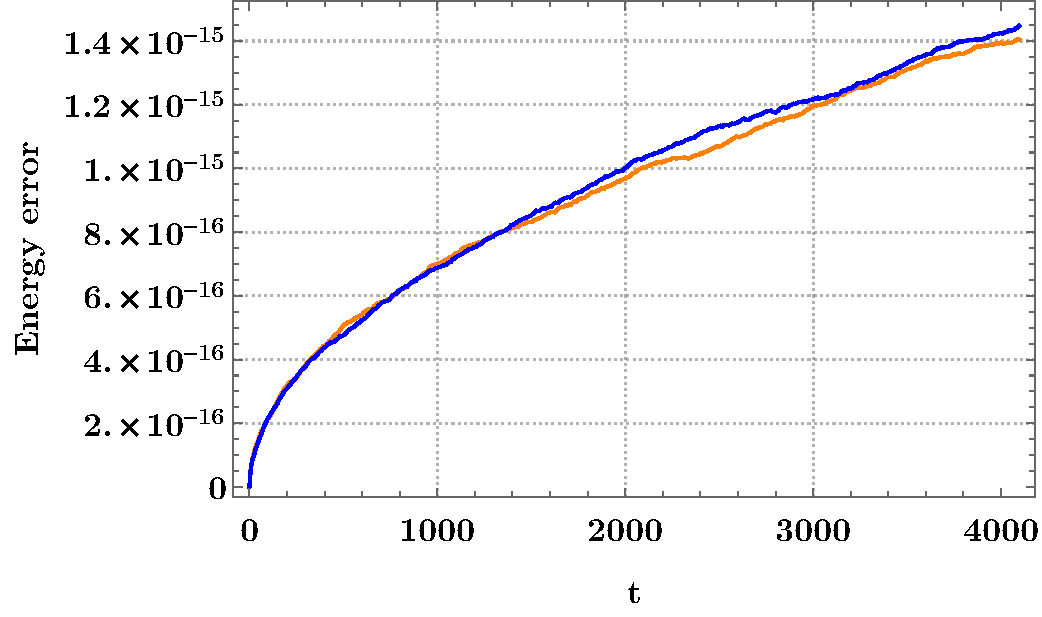
\includegraphics[width=.4\textwidth]{Fig3N}}
\\
\subfloat[$k=2^{10}$ energia errorrearen batezbestekoa]
{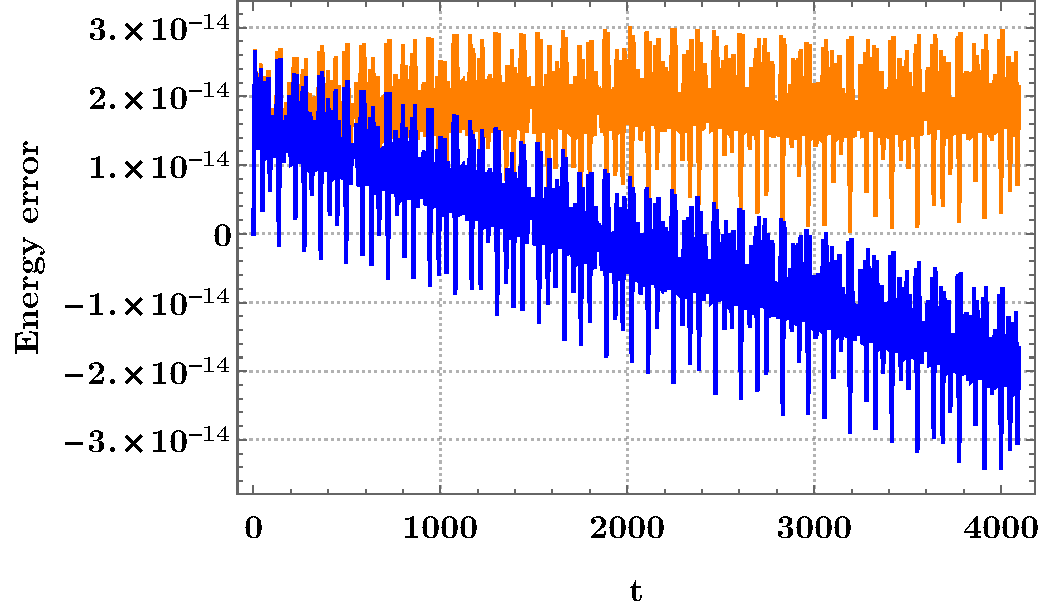
\includegraphics[width=.4\textwidth]{Fig4N}}
&
\subfloat[$k=2^{10}$ energia errorearen desbideratze estandarra]
{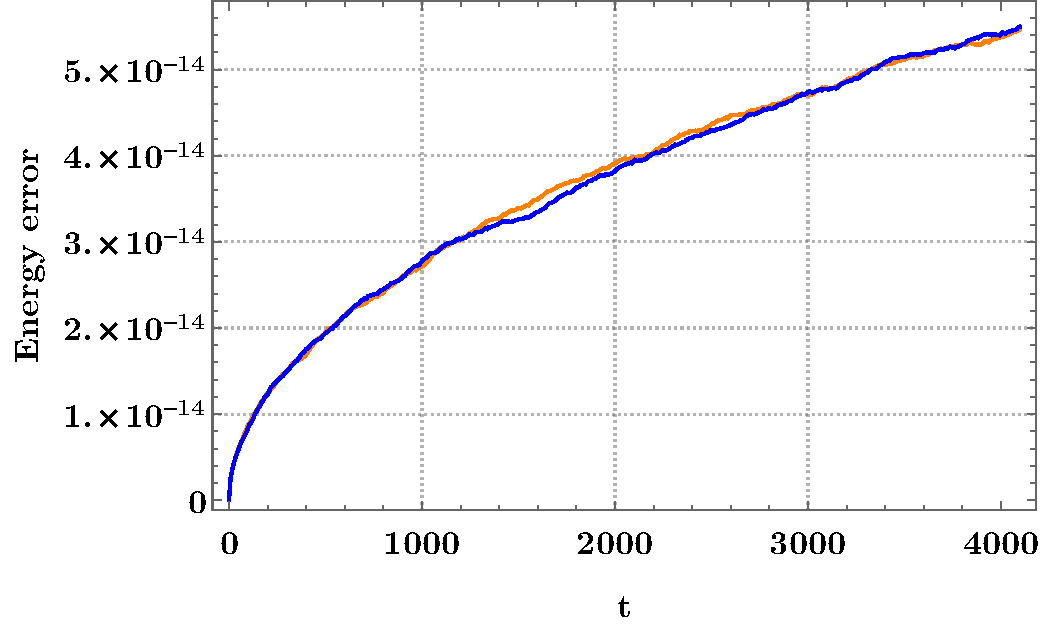
\includegraphics[width=.4\textwidth]{Fig5N}}
\\
\subfloat[$k=2^{12}$ energia errorrearen batezbestekoa]
{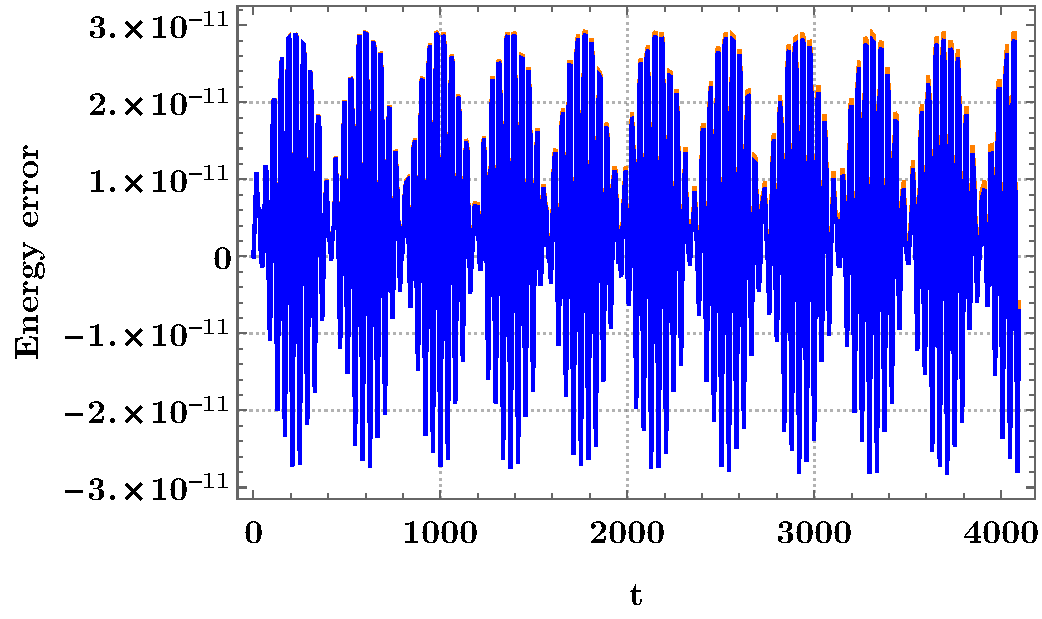
\includegraphics[width=.4\textwidth]{Fig6N}}
&
\subfloat[$k=2^{12}$ energia errorearen desbideratze estandarra]
{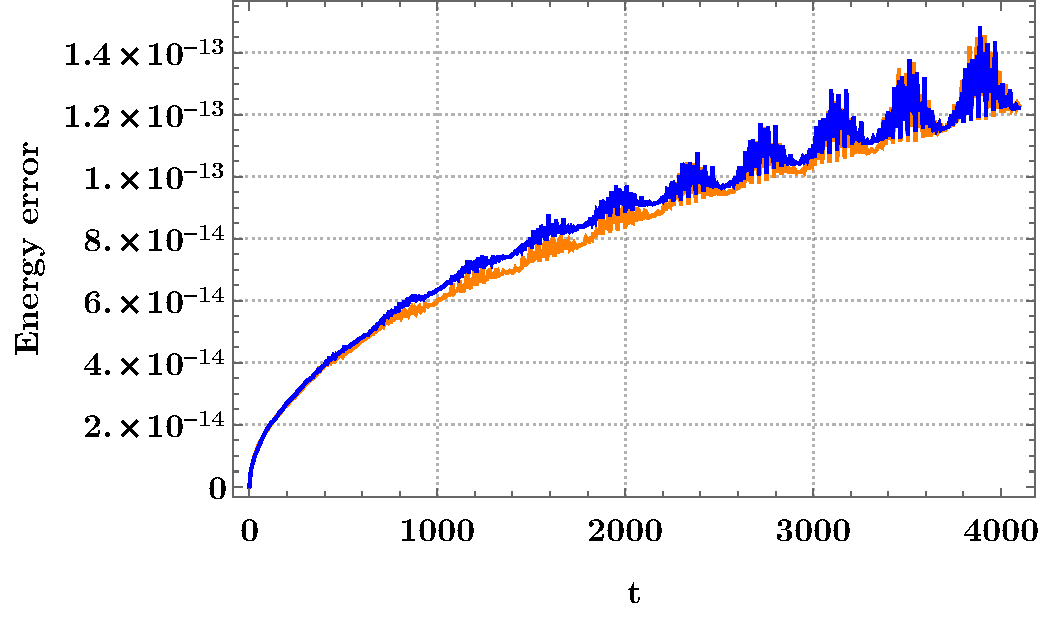
\includegraphics[width=.4\textwidth]{Fig7N}}
\end{tabular}
\caption{\small Energia errorearen batezbestekoaren (ezkerrean) eta desbideratze estandarraren  eboluzioa (eskubian), puntu-finkoaren inplementazioa (urdinez), eta  Newton inplementazioa (laranjaz). $k=0$ problema ez-zurruna (a,b), $k=2^{10}$ lehen problema zurruna (c,d) eta $k=2^{12}$ bigarren problema zurruna (e,f)}
\label{fig:plot3}
\end{figure}


\subsection{Puntu-finkoa versus Newton iterazioa}


\ref{tab:fp1} taulan, $k$ parametroaren lau balioetarako, bi inplementazioen eraginkortasunaren adierazle nagusienak laburtu ditugu.

\begin{table}[h!]
\caption[Fixed-point percentage of steps and mean iterations.] 
{}
\label{tab:fp1}       % Give a unique label
\centering
{%
\begin{tabular}{ l l l l l } 
 \hline
%                 &  \multicolumn{2}{c}{FPIEA}  & \multicolumn{2}{c}{DP} & \multicolumn{2}{c}{Hairer} \\
\\
 $k$               & $0$  & $2^3$ & $2^6$ & $2^8$ \\
 $E_0$           & $-14.39$  & $-5.75$ & $-5.64$ & $-5.64$ \\ 
\\
 \hline
\\
 Fixed-points it.&           &         &         &         \\
 \cline{1-1}     &           &         &         &         \\
 Elapsed-time (sec.)    & $10$      & $12$    & $19$    & $51$    \\ 
 It. per step    & $8.58$    & $11.1$  & $22.$  & $64.2$  \\
 Energy          & $2.96\times 10^{-15}$ & $1.81\times 10^{-14}$ & $2.94\times 10^{-11}$ & $6.33\times 10^{-5}$ \\
 \\
 Newton it.            &           &         &         &         \\
 \cline{1-1}           &           &         &         &         \\
 Elapsed-time (sec.)   & $18$      & $20$    & $19$    & $18$     \\
 It. per step          & $5.09$    & $5.53$  & $5.58$  & $5.01$   \\
 L. solves per step    & $11.37$   & $12.92$  & $12.72$  & $11.04$ \\
 Energy                & $1.6\times 10^{-15}$ & $1.74\times 10^{-14}$ & $2.94\times 10^{-11}$ & $6.33\times 10^{-5}$ \\   
 \\  
   \hline
 \end{tabular}}
\end{table}

Eraginkortasuna neurtzeko, bi inplementazioen exekuzio sekuentzialen cpu-denborak  konparatu ditugu. Horrez gain, bi inplementazioen urratseko iterazioen batezbestekoak (It. per step) alderatu ditugu eta Newton inplementazioan, urratseko sistema linealen ebazpenen batezbestekoa (L.solves per step) eman dugu. Zenbakizko soluzioaren doitasuna neurtzeko, energiaren errore erlatiboaren maximoa eman dugu,
\begin{equation*}
\max | \frac{E(t_n)-E(t_0)}{E(t_0)}|, \ \  t_n=t_0+nh, \ \ n=1,2,\dots
\end{equation*} 

$k$ balio txikienetarako, puntu-finkoaren inplementazioa Newton inplementazioa baino eraginkorragoa da. Baina, pendulu bikoitzaren zurruntasun maila handitzen dugunean, puntu-finkoaren iterazio kopurua gero eta handiagoa den bitartean, Newton inplementazioaren iterazio kopurua mantendu egiten den, eta $k$ handietan txikitu ere bai. Beraz, zurruntasuna handitzen dugunean, Newton inplementazioa gero eta eraginkorragoa bilakatzen da. $k=2^{18}$ baliotik aurrera, puntu-finkoak ez du konbergitzen eta Newton inplementazioak, antzeko iterazio kopuruarekin konbergitzen du.

 
%\small{Percentage of steps that reach a computational fixed-point and the number of fixed-point iterations per step for the computations of  double pendulum stiff problem}



\section{Laburpena.}

IRK metodoen Newton sinplifikatuaren iterazioen ekuazio-sistema, modu eraginkorrean askatzeko inplementazioa proposatu dugu. Newtonen iterazioan oinarritutako IRK metodoaren inplementazio berria aurkeztu dugu eta inplementazio honen biribiltze errorearen hedapena egokia dela baieztatu dugu. Problema zurrunetarako, Newton sinplifikatuaren iterazioa, puntu-finkoaren iterazioa baino eraginkorragoa dela ikusi dugu.

Newtonen iterazioan oinarritutako IRK metodoen inplementazioen inguruko lan hauek aipatuko ditugu: "On the implementation of implicit Runge-Kutta methods", J.C. Butcher \cite{Butcher1976}, "Geometric numerical integration: structure-preserving algorithms for ordinary differential equations", E.Hairer et al \cite{Hairer2006}.

Azkenik, aipatu nahi dugu, atal honen edukiak \href{http://link.springer.com/journal/11075}{Numerical Algorithms} aldizkarian publikatutako \cite{Antonana2017a} artikuluan aurki daitezkeela eta inplementazioaren \href{https://github.com/mikelehu/IRK-Newton}{kodea} eskuragarri jarri dugula.

\chapter{IRK: Eguzki-sistema.}


\section{Sarrera.}
  

Kapitulu honetan, eguzki-sistemaren ekuazio diferentzialei Kepler-en fluxuan oinarritutako aldagai aldaketa aplikatzea proposatuko dugu. \ref{chap:IRK-PF}. kapituluan puntu-finkoaren iterazioan oinarrituz eta \ref{chap:IRK-NEW}. kapituluan Newton sinplifikatuaren iterazioan oinarrituz IRK inplementazioak garatu ditugu; eguzki-sistemaren problemaren integraziorako, bi inplementazioen artean, puntu-finkoarena eraginkorragoa dela baieztatu dugu. Hortaz, puntu-finkoaren iterazioan oinarritutako IRK inplementazioa erabiliko dugu eta  ekuazio diferentzialetako aldagaiei eragingo diegun aldagai aldaketaren bidez, integrazio eraginkorra lortzea espero dugu.  

Aplikatzen dugun integrazio metodoa sinplektikoa eta simetrikoa da: neurri batean, Splitting metodoen baliokidea. Aldagai berriekiko ekuazio diferentzialak, magnitude txikiko balioak hartzen dituzte eta honek, hiru abantaila eragingo ditu. Lehenik, eguzki-sistemaren problemaren trunkatze errore nagusiena ezabatzen dugunez, urrats luzera handiagoak erabili ahal izango ditugu. Bigarrenik, batura konpensatuaren konputazioan, informazio gutxiago galduko dugu. Jacobiarraren balioa txikia denez, puntu-finkoaren iterazioek konbergentzia azkarra izango dute. 

Lehenengo, Kepler-en fluxuaren inplementazioa azalduko dugu. Bigarrenik, aldagai aldaketa definitu eta metodoa integratzeko zehaztapenak emango ditugu. Hirugarrenik, eguzki-sistemaren problemaren zenbakizko integrazioak egingo ditugu: inplementazio honen eta doitasun altuko beste metodo sinplektikoen eraginkortasunak, alderatuko ditugu.     

 

\section{Kepler-en fluxua.}
   
   
Kepler problema bi gorputzen problemaren kasu partikularra da eta  honako Hamiltondarra dagokio,
\begin{equation}
\label{eq: hamkepler}
H(q,p)=\frac{p^2}{2m}-\frac{\mu}{\|q\|},
\end{equation}
non $m$ eta $\mu$ konstanteen balioak, formulazioaren araberakoak diren.

Koordenatu sistema $q=q_2-q_1$ duen formulazioa aukeratzen badugu, konstanteen balioak hauek dira,  
\begin{equation*}
m=(1/m_1+1/m_2)^{-1},\ \ \mu=Gm_1m_2,
\end{equation*} 
%
eta ekuazio diferentzialak era honetan definitzen dira,
\begin{equation}
\label{eq:kode}
\dot{q}=p, \ \ \dot{p}= - \frac{k \ q}{\|q\|^3} ,
\end{equation}
non $k= \mu / m$ eta  $q,p \in \mathbb{R}^3$.

Kepler problemaren soluzio zehatza kalkula daiteke: une bateko kokapen eta abiadurak emanik, $\Delta t$ denbora tarte bat igarotakoan (positiboa ala negatiboa), kokapen eta abiadura zehatzak konputatu daitezke. Eguzki-sistemaren integrazio metodoentzat, Kepler problema doitasun handian eta era eraginkorrean kalkulatzea, funtsezkoa da. Kepler problemaren erreferentziazko inplementazioak, Danby \cite{Danby1992} eta J.Wisdom-enak  \cite{Wisdom2015} ditugu. 

Kepler-en fluxua, era honetan kalkulatzen da. Lehenik, koordenatu cartesiarretatik ($q,p\in \mathbb{R}^3$), koordenatu eliptikoetara $(a,e,i,\Omega,E)$ itzulpena egingo dugu. Koordenatu eliptikoetan, $E$ (\emph{eccentric anomaly}) aldagaia izan ezik, beste aldagaiak konstante mantentzen dira: beraz $E_0$ balioa emanda, $\Delta t$ denbora tartea aurrera egin eta $E_1$ balio berria kalkulatuko dugu. Azkenik, koordenatu eliptikoetatik koordenatu cartesiarretara itzulpena eginez, kokapen eta abiadura berriak eskuratuko ditugu. 

\begin{equation*}
(q_0,v_0) \in \mathbb{R}^6 \ \ \ \longrightarrow \ \ \  (a,e,i,\Omega,E_0) \in \mathbb{R}^6 
\end{equation*}
\begin{equation*}
\quad \quad \quad \quad \quad \quad \quad \quad \downarrow \Delta t
\end{equation*}
\begin{equation*}
(q_1,v_1) \in \mathbb{R}^6 \ \ \ \longleftarrow \ \ \  (a,e,i,\Omega,E_1) \in \mathbb{R}^6 
\end{equation*}

Gorputz baten orbita Kepleriarra hiru motakoa izan daiteke: $H(q_0,p_0)<0$ denean orbita eliptikoa da, $H(q_0,p_0)>0$ orbita hiperbolikoa eta $H(q_0,p_0)=0$ orbita  parabolikoa. Kepler fluxuaren C inplementazioa, orbita eliptikoetarako garatu dugu eta zehaztasunak, \ref{erans:B1} eranskinean eman ditugu. (\ref{eq:kode}) problemari dagokion fluxua, era honetan defini daiteke,
\begin{align*}
\varphi_{\Delta t}^k:&  \quad \mathbb{R}^{6} \quad  \longrightarrow \quad \mathbb{R}^6,  \\
&  \quad u_0 \ \  \rightsquigarrow \ \ u_1. 
\end{align*} 
non $u=(q,v) \in \mathbb{R}^6$  den.

\section{Kepler Perturbatuaren problema.}

Kepler problemaren Hamiltondarra perturbatzen badugu ezingo dugu aurreko atalean erabili dugun fluxua erabili problema ebazteko. Kasu honetan Hamiltondarra  bi zatitan banatuta egongo da;
\begin{align}
\begin{split}
\label{eq: hamkeplerpert}
&H(q,p,t)=H_K(q,p)+H_I(q,p,t)
\end{split}
\end{align} 
non $H_K$ mugimendu Kepleriarrari dagokion Hamiltondarraren aldea den, hau da, (\ref{eq: hamkepler}) ekuazioko eskuin aldea, eta $H_I$ perturbazioei dagokien Hamiltondarraren aldea den.

Problema berri honetan aldagai aldaketa bat egingo dugu, aldaketaren helburua da keplerren fluxua eabili ahal izatea problemaren ebazpenean. 

\subsection*{Aldagai aldaketa.}

%Kontutan hartuko ditugun sistemak Hamiltondarrak dira, $H: \mathbb{R} \times \mathbb{R}^{2d} \longrightarrow \mathbb{R}$, gainera, Hamiltondarra bi zatitan bana dakieken sistemak hartuko ditugu kontuan:


(\ref{eq: hamkeplerpert}) problemari dagozkion ekuazioetan Keplerren fluxuan oinarritutako aldagai aldaketa bat egingo dugu, baina horretarako notazioa finkatuko dugu: jatorrizko aldagaiak $u=(q,p) \in \mathbb{R}^{2d}$ izango dira eta aldagai berriak $U=(Q,P) \in \mathbb{R}^{2d}$ letra larriz adieraziko ditugu. Jatorrizko aldagaien bidez adierazitako problema, alegia, ebatzi beharreko hasierako baliodun problema, honakoa da:

\begin{align}
\begin{split}
\label{eq: HamEDA}
&\frac{du}{dt} = k(u) + g(u,t),\ \ \ u(0) = u_0
\end{split}
\end{align} 
non $k(u)$ alde kepleriarrari dagokion eta $g(u,t)$ perturbazioari. 
Problema horretan honako aldagai aldaketa egingo dugu, kontuan izan urrats bakoitzean egingo dugula aldagai aldaketa, hau da $j=0, 1, 2 \ldots$ indizeak $j$. urratsean aplikatu beharreko aldaketa adierazten du:

\begin{align}
\begin{split}
\label{eq: uUaldaketa}
&u(t) = \varphi_{t-(j+\frac{1}{2})h}^k\left(U_j^{j+\frac{1}{2}}(t)\right)
\end{split}
\end{align} 
$\varphi_{\Delta t}^k$ fluxua $\Delta t>0$ eta $\Delta t <0$ balioentzat definitzen da, eta  $u= \varphi_{-t}(\varphi_{t}(u))$ betetzen dela kontutan hartuz honako alderantzizko aldaketa ere egin dezakegu:
\begin{align}
\begin{split}
\label{eq: Uualdaketa}
U^{j+\frac{1}{2}}(t) = \varphi^k_{-t+(j+\frac{1}{2})h} \left( u(t) \right)
\end{split}
\end{align} 

Aldaketa hauekin asmoa da $i+1$ urratsa emateko $u_i \approx u(hi)$ zenbakizko soluzioan oinarrituz, aldagai aldaketaren bidez $U_i^{i+\frac{1}{2}}=\varphi^k_{\frac{h}{2}}(u_i)$ lortu, hau da, fluxuan $\frac{h}{2}$ aurrera egin aldagai berriak lortzeko, aldagai berri hauetan ebatzi jatorrizko problemaren urrats bati dagokion zenbakizko soluzioa (ikusiko dugun bezala, aldagai berrietan alde kepleriarrari dagokion espresioak ez du eraginik eta, azken finean perturbazioari dgokion aldaketa da hemen kalkulatuko dena) eta azkenik, aldagai berri hauen balio berriak jatorrizko aldagaietara itzuli behar dira, baina $i+1$ urratsari dagozkion unera pasa behar dira aldagaiak, hau da, fluxuan aurrera $\frac{h}{2}$ egin behar da. Atzera egingo bagenu urratsaren hasierako balioei perturbazioak zein aldaketa eragiten dien kalkulatuko baikenuke, baina guk urratsaren bukaerako balioak nahi ditugu. Laburbilduz:


\begin{align*}
   &   \quad U_0^{\frac{1}{2}} \quad \quad \quad \quad \Longrightarrow  & U_1^{\frac{1}{2}}&  &\\
  & \nearrow \varphi_{\frac{h}{2}}(u_0) &            & \searrow \varphi_{\frac{h}{2}}(U_1)& \\
u_0 &                  &    &\quad \quad \quad  u_1
\end{align*}

Aldagai aldaketak fluxuan aurrera egiten du urratsaren luzeraren erdia. Hori horrela egiteak badu arrazoi bat: urratsa bere osotasunean simetrikoa da. Aurrera $h$ luzerako urratsa ematea $-h$ luzerako urratsa ematearekin desegiten baita. 

%\begin{figure}[h!]
%\centering
%\subfloat[Aldagai aldaketa.]{
%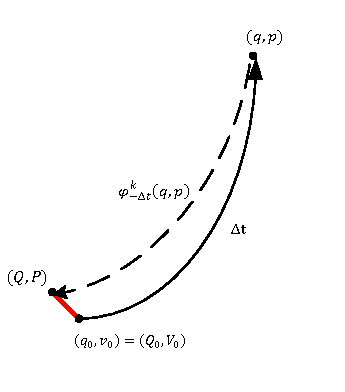
\includegraphics[width=.400\textwidth]{Aldagaialdaketa1}
%}
%\subfloat[Aldagai berrien integrazioa.]{
%\includegraphics[width=.400\textwidth]{Aldagaialdaketa2}
%}
%\caption[Atalen hasieraketa.]
%        {\small (a)irudian, aldagai aldaketa irudikatu dugu eta (b) irudian, perturbatutako gorputza baten orbitaren integrazioak erakutsi ditugu. Bi irudietan, $(Q,P)$ balioen aldaketa txikiak gorriz nabarmendu ditugu          
%        }
%\label{fig:Aldg}
%\end{figure}   

\subsection*{Aldagai berrietan ekuazio diferentzialak.}

(\ref{eq: uUaldaketa}) aldagai aldaketa abiapuntutzat hartuz, aldagai berriei dagozkien ekuazio diferentzialak lortu behar ditugu. Horrela, problemaren integrazioa aldagai berrien arabera egin ahal iango dugu. Irakur erraztasunagatik (\ref{eq: uUaldaketa}) ekuazioko $\varphi(U)$ indizerik gabe idatziko dugu, eta $\dot{U}$ri dagozkion ekuazioak lortze aldera bi aldeak $t$ aldagaiarekiko deribatuko ditugu:  
\begin{align}
\begin{split}
&\frac{d}{dt}u = \frac{d}{dt}\left(\varphi(U)\right),
\end{split}
\end{align}
Eskuin aldeari katearen erregla aplikatuz, 
\begin{align}
\begin{split}
&\dot{u} = \dot{\varphi}(U) + \varphi'(U) \frac{d}{dt}U.
\end{split}
\end{align}
$\varphi$ Kepler problemaren fluxua da, hau da, $\dot{u} = k(u)$ problemaren fluxua da, eta fluxuaren definizioz $\dot{\varphi}(U) = k(\varphi(U))$ da. Aldaketa horrekin,  eta (\ref{eq: HamEDA}) ekuazioarekin berdinduz,
\begin{align}
\begin{split}
&k(u) + g(u,t) = k(u) + \varphi'(U) \dot{U}.
\end{split}
\end{align}
Bi aldeetan $k(u)$  kenduz, $U$ aldagaiekiko ebatzi beharreko ekuazio diferentziala lortuko dugu:
\begin{align}
\begin{split}
\label{eq:hamEDAU}
&\dot{U} = \left(\varphi'(U)\right)^{-1} g(u,t).
\end{split}
\end{align}
Alderantzizko matrizeak kalkulatu beharrik gabe idatz ditzakegu (\ref{eq:hamEDAU}) ekuazioak. Horretarako $\varphi$ fluxuaren izaera sinplektikoa erabiliko dugu, hau da, $(\varphi')^tJ\varphi'= J$ propietatea betetzen du fluxuak, ondorioz,
%
\begin{align}
\begin{split}
\label{eq:hamEDAU2}
&\dot{U} = J^{-1}(\varphi')^{t}(U)J g(u,t).
\end{split}
\end{align}
(\ref{eq:hamEDAU2}) ekuazioak $\varphi'(U)$ kalkulatzea eskatzen du, eta horretarako deribazio automatikoko teknikak erabil ditzakegu


\paragraph*{Algoritmoa.}
$U$ aldagaietan oinarritutako ekuazio diferentzialen integraziorako (\ref{eq:hamEDAU2}) espresioaren konputazioa hiru urratsetan egingo dugu:
\begin{enumerate}
\item $\{u,aux\} \leftarrow KeplerFlowGen (t,U,mu)$.

Kepler-en fluxua $(q,v)= \varphi_t(U)$ aplikatuko dugu eta fluxuaren kalkulutarako erabilitako tarteko balioak, ~$aux\in \mathbb{R}^{16}$ aldagaian itzuliko ditugu. 

\item $g \leftarrow g(u,t)$.

Jatorrizko problemako ekuazio diferentzialetan perturbazioei dagokien espresioa kalkulatuko dugu.

\item $KeplerFlowGFcnaux(aux,U,t,g)$.

Urrats honetan $\varphi'_t())$ kalkulatu behar da. Deribazio automatikoaren tekniken bidez, Kepler fluxuaren $U$ aldagaiekiko deribatuaren konputazio eraginkorra definitu dugu. 

Hirugarren urratsak (\ref{eq:hamEDAU2}) espresioa konputatzeko behar dugun azken zatia kalkultzen du, beraz, bere emaitza $\dot{U}$ren konputazioa izango da: 
\begin{align*}
\dot{U}&\leftarrow KeplerFlowGFcnaux(aux,U,t,g) \left(= ( \varphi'(U))^{-1} \ g\right).
\end{align*}

\end{enumerate} 



\section{Alde Kepleriar bat baino gehiagoko sistemak.}

Alde Kepleriar bat baino gehiago dituzten problemetan ere Kepler perturbatuan egindako aldagai aldaketa egin dezakegu. Hainbat gorputzeko sisteman gorputz bakoitzari eragingo diogu aldagai aldaketa, bakoitzak bere fluxu kepleriar perturbatua izango du, eta horretan oinarrituz egingo diogu aldaketa. Problemaren alde Kepleriarren kopurua $k$ bada, era honetako ekuazio diferentzialak ditugu,
\begin{equation}
\label{eq: n-pertEDA}
\frac{d}{dt}\left(\begin{array}{c}
                u  \\
                w  \\
\end{array}\right)=
\left(\begin{array}{c}
                \dot{u}_1  \\
                \dot{u}_2  \\
                \vdots \\
                \dot{u}_k    \\
                \dot{w}      \\
\end{array}\right)=
\left(\begin{array}{c}
                k(u_1)  \\
                k(u_2)  \\
                \vdots \\
                k(u_k)  \\
                0      \\
\end{array}\right)+
\left(\begin{array}{c}
      g_1(u_1, u_2\dots, u_k,w,t) \\
      g_2(u_1, u_2\dots, u_k,w,t) \\
                \vdots \\
      g_k(u_1, u_2\dots, u_k,w,t)\\
      g_{k+1}(u_1, u_2\dots, u_k,w,t)
\end{array}\right)
\end{equation} 

Gorputz bakoitzari dagokion aldagai aldaketa bere fluxu kepleriarraren arabaerakoa da,
\begin{align}
\label{eq:aldfl2}
\begin{split}
u_j&= \varphi_t^{k_j}(U_j), \ \ \ j=1,\dots,k.
\end{split}
\end{align}
Bi aldeak $t$ aldagaiarekiko deribatuz eta katearen erregla aplikatuz,
\begin{equation*}
\left(\begin{array}{c}
                \dot{u}_1  \\
                \dot{u}_2  \\
                \vdots \\
                \dot{u}_k    \\
                \dot{w}      \\
\end{array}\right)=
\left(\begin{array}{c}
                \dot{\varphi}^1(U_1)  \\
                \dot{\varphi}^2(U_2)   \\
                \vdots \\
                \dot{\varphi}^k(U_k)   \\
                0      \\
\end{array}\right)+
\left(\begin{array}{c}
      \varphi'^1(U_1) \frac{d}{dt}U_1 \\
      \varphi'^2(U_2) \frac{d}{dt}U_2 \\
                \vdots \\
     \varphi'^k(U_k) \frac{d}{dt}U_k\\
      g_{k+1}(u_1, u_2\dots, u_k,w,t)
\end{array}\right),
\end{equation*}
ekuazioetan fluxuen propietate eta definizioak erabiliz,
\begin{equation*}
\left(\begin{array}{c}
                \dot{u}_1  \\
                \dot{u}_2  \\
                \vdots \\
                \dot{u}_k    \\
                \dot{w}      \\
\end{array}\right)=
\left(\begin{array}{c}
                k(u_1)  \\
                k(u_2)   \\
                \vdots \\
                k(u_k))   \\
                0      \\
\end{array}\right)+
\left(\begin{array}{c}
      \varphi'^1(U_1) \dot{U}_1 \\
      \varphi'^2(U_2) \dot{U}_2 \\
                \vdots \\
     \varphi'^k(U_k) \dot{U}_k\\
      g_{k+1}(u_1, u_2\dots, u_k,w,t)
\end{array}\right),
\end{equation*}
eta, azkenik, (\ref{eq: n-pertEDA}) ekuazioarekin berdinduz eta sinplifikatuz,
\begin{equation*}
\left(\begin{array}{c}
                \dot{U}_1  \\
                \dot{U}_2  \\
                \vdots \\
                \dot{U}_k    \\
                \dot{w}      \\
\end{array}\right)=
\left(\begin{array}{c}
      \left((\varphi'^1(U_1)\right)^{-1} g_1 \\
      \left(\varphi'^2(U_2)\right)^{-1} g_2 \\
                \vdots \\
     \left(\varphi'^k(U_k)\right)^{-1} g_k\\
      g_{k+1}
\end{array}\right),
\end{equation*}

Aldagai berriekiko ekuazio diferentzialak balioztatzeko, fluxuen propietateei esker,$(\varphi')^{-1}=J^{-1}(\varphi')^tJ$ kalkula dezakegu eta, Kepler perturbatuan bezalaxe, alderantzizko matrizerik kalkulatu beharrik ez dugu izango. Deribazio automatikoko teknikei esker, kalkulatu ahal izango ditugu. Bestalde, $\dot{w}$ aldagaien ekuazioak balioztatzeko $u_i$ aldagaiak behar ditugu, baina $U_i$ aldagaietatik lor ditzakegu, gainra, $g_i$ funtzioetarako ere behar ditugu. Ondorioz, Kepler perturbatuaren probleman bezala hiru urratsetan balioztatu ahal izango ditugu ekuazioak.



\subsection*{Metodo simetrikoa.}

Azpimarratu behar dugu aldagai aldaketa urratsero egiten dugula, eta ekuazio diferentziala aldagai berriekiko ebazten dugula. Aldagai berriak eta jatorrizko aldagaiak fluxuak erlazionatzen ditu: jatorrizko aldagaiak fluxuan $\frac{h}{2}$ aurrera eginez aldagai berriak lor ditzakegu. Ebatzi beharreko problema aldagai berrietan ebatziko dugu, eta $h$ luzerako urratsa emanez aldagai berriak aldatuko ditugu. Jatorrizko aldagaietara igarotzeko fluxuaren bidez mugitu behar ditugu balio horiek: $\frac{h}{2}$ atzera egiten badugu jatorrizko aldagaiak urratsaren hasieran kokatuko ditugu, baina perturbazioari dagokion aldaketa bere baitan daramate, izan ere, aldagai berriei metodoaren urratsa kalkulatu diegu, hau da, perturbazioari dagokion $h$ luzerako urratsa eman dugu. Bestalde, fluxuan $\frac{h}{2}$ aurrera egiten badugu hurrengo urratsaren hasierako egoerara eramango ditugu balioak.

Ondorioz integrazioko urrats bat hiru azpiurratsen konbinazioa da:
\begin{enumerate}
\item $U_i^{i+\frac{1}{2}}=\varphi_{\frac{h}{2}}(u_i)$: fluxuaren arabera $\frac{h}{2}$ aurreratu.
\item Gauss metodoaren $h$ luzerako urratsa: $U_i^{i+\frac{1}{2}}$ aldagaietatik  $U_{i+1}^{i+\frac{1}{2}}$ balioetara pasako gara.
\item $u_{i+1}=\varphi_{\frac{h}{2}}(U_{i+1}^{i+\frac{1}{2}})$ fluxuaren araberako $\frac{h}{2}$ aurreratu.
\end{enumerate}

Hiru azpiurratsak simetrikoak dira, eta ondorioz, $u_{i+1}$ abiapuntutzat hartuz, $-h$ luzerako urratsa ematen badugu $u_i$ lortuko dugu:
\begin{enumerate}
\item $\varphi_{\frac{-h}{2}}(u_{i+1})$ kalkulatu behar da, baina $u_{i+1}$ hirugarren azpiurratsaren emaitza denez, bere espresioa jarriko dugu, eta ikusiko dugu $U_{i+1}^{i+\frac{1}{2}}$ aldagaietatik hasi eta fluxuan aurrera eta atzera egitearen parekoa dela, alegia, ez aldatzearen parekoa:
\[
U_{i+1}^{i+1+\frac{1}{2}}=\varphi_{\frac{-h}{2}}(u_{i+1})=\varphi_{\frac{-h}{2}}\left(\varphi_{\frac{h}{2}}(U_{i+1}^{i+\frac{1}{2}}) \right)
= U_{i+1}^{i+\frac{1}{2}}
\] 
\item Gauss metodoaren $-h$ luzerako urratsa: Gaussen metodoa simetrikoa denez, aurreko urratsean bukaerako egoera zenari $-h$ luzerako urratsa eragiteak hasierako egoera itzultzen du, beraz, $(U_{i+1}^{i+\frac{1}{2}}$ balioetatik abiatuz $U_i^{i+\frac{1}{2}}$ balioetara itzuliko gara.
\item Fluxuan urrats luzeraren erdia egin behar da: lehenengo azpiurratsean bezala, fluxuan $\frac{-h}{2}$ mugitu behar gara, baina fluxuan $\frac{h}{2}$ mugitutako balioekin egin behar dugu, hau da:
\[
\varphi_{\frac{-h}{2}}(U_i^{i+\frac{1}{2}}) = \varphi_{\frac{-h}{2}}\left(\varphi_{\frac{h}{2}}{u_i}) \right) = u_i
\]
\end{enumerate}

Metodoa integrazio eskema orokorra \ref{fig:proiekzioa0}~irudian laburtu dugu, bere simetria ere bertan ikus daiteke,
\begin{figure} [h!]
\centerline{\includegraphics [width=16cm, height=4cm] {proiekzioa11}}
\caption{}
\label{fig:proiekzioa0}
\end{figure} 

Integrazioaren urrats guztietan ez baditugu emaitzak itzuli behar, bi urratsen arteko, $\varphi_{h/2}$ fluxuaren bi konputazioak, $\varphi_{h}$ fluxuaren konputazio bakarrarekin konputatuko dugu. Horretarako, proiekzio kontzeptua sortuko dugu (\ref{fig:proiekzioa2}~irudia).

\begin{figure} [h!]
\centerline{\includegraphics [width=14cm, height=4cm] {proiekzioa12}}
\caption{\small Proiekzioa: bi urratsen arteko, $\varphi_{h/2}$ fluxuaren bi konputazioak, $\varphi_{h}$ fluxuaren konputazio bakarrarekin konputatuko dugu}
\label{fig:proiekzioa2}
\end{figure} 


 Azkenik, emaitzak behar ditugun urratsetarako fluxua $\varphi_{-h/2}$ aplikatuko dugu (\ref{fig:proiekzioa1}~irudia). 

\begin{figure} [h!]
\centerline{\includegraphics [width=14cm, height=4cm] {proiekzioa1}}
\caption{\small $u_i$ jatorrizko aldagaiak eta $U_i$ aldagai berriak adierazten dute. Lehenengo, $u_0$ jatorrizko aldagaien hasierako baliotik abiatuta, aldagai berriei dagokion hasierako balioa finkatuko dugu $(U_0,-h/2)$. Urrats bakoitza, integrazio eta proiekzioaren konposaketa da eta \ref{fig:proiekzioa2} irudian zehaztu dugu. Erabiltzaileak definitutako urratsetarako, $u_n$ jatorrizko aldagaietann zenbakizko soluzioa itzuliko dugu}
\label{fig:proiekzioa1}
\end{figure} 


$u_i$ jatorrizko aldagaiak eta $U_i$ aldagai berriak adierazten duten notazioa erabiliko dugu. Hauek dira, integratzeko emango ditugun urratsak:
\begin{enumerate}
\item \emph{Startfun} funtzioa.

Lehenengo, $u_0$ jatorrizko aldagaien hasierako baliotik abiatuta, $\varphi_{h/2}$ fluxuaren konputazioaren bidez, aldagai berrietan dagokion hasierako balioa lortuko dugu.
\begin{align*}
u_0 \ \rightarrow \ U_0^{\frac{1}{2}}.
\end{align*}

\item \emph{Urratsa}.

Urratsa bi azpiurratxen konbinazio bezala ikusiko dugu: aldagai berriei Gaussen metodoaren bidezko integrazioaren urrats bat eta lortutemaitzei $\varphi_{h}$ bidez fluxuan $h$ aurrera egitea. Bigarren azpiurratsa fluxuaren bidez proiektatzea da. \ref{fig:proiekzioa2} irudian zehaztapenak eman ditugu. 
\begin{align*}
 U_0^{\frac{1}{2}} \ \rightarrow \ U_1^{\frac{1}{2}} \rightarrow \ U_1^{1+\frac{1}{2}}.
\end{align*}

Biribiltze errorea txikitzeko, proiekzioa doitasun altuan konputatzea garrantzitsua da. Modu honetan, batura konpensatua aplikatzerakoan zifra batzuk irabaziko ditugu. 

\item \emph{Outputfun} funtzioa.

Erabiltzaileak $t$ren balio jakin batzuetan $u(t)$ balioen zenbakizko soluzioak nahiko ditu, kasu horietan $\varphi_{-h/2}$ fluxuaren konputazioaren bidez, $U_i^{i+\frac{1}{2}}$ balioetatik $u_i$ jatorrizko aldagaien balioak lortu beharko dira:
\begin{align*}
U_n^{n+\frac{1}{2}} \ \rightarrow \ u_n.
\end{align*}


\end{enumerate}


Gauss metodoa, neurri batean  Splitting eta konposizio metodoen baliokideak dira. 
\begin{align*}
&\text{Konposizio metodoa} \ \ \Leftrightarrow \ \ \text{Gauss metodoa aldagai aldaketa gabe}.\\
&\text{Splitting metodoa}  \ \ \Leftrightarrow \ \  \text{Gauss metodoa aldagai aldaketarekin}.
\end{align*}

Splitting metodoekiko antzekotasuna azaltzeko, (\ref{eq:stverlet})~\emph{Störmer-Verlet} Splitting metodoarekin konparatuko dugu. \emph{Störmer-Verlet} metodoa, era honetan aplikatzen da: $h/2$ fluxua aplikatu, perturbazioak kalkulatu eta berriz  $h/2$ fluxua aplikatu. Fluxuaren aldagai aldaketarekin, gauza bera egiten ari gara: $h/2$ fluxua aurreratu, perturbazioak kalkulatu (aldagai berrietan eta beraz, hobeto kalkulatzen dugu), $h/2$ fluxua aurreratu. 


\section{Zenbakizko esperimentuak.}
\label{s:7espmt}

Zenbakizko esperimentuetarako, puntu-finkoaren iterazioan oinarritutako Gauss metodoaren inplementazioa (\ref{chap:IRK-PF}~kapitulua) erabili dugu eta eguzki-sistemaren ekuazio diferentzialei, Kepler-en fluxuan oinarritutako aldagai aldaketa aplikatu diegu. $s=6,8,9,16$ ataletako Gauss metodoak exekutatu ditugu eta metodo eraginkorrena aukeratu dugu, \emph{CO1035} konposizio eta \emph{ABAH1064} Splitting  metodoekin konparatzeko.

Esperimentu hauen konputaziorako, $64$-biteko (bikoitza) eta $80$-biteko (\emph{long double}) doitasunak nahasi ditugu. Konputazioaren zati nagusiena, $64$-biteko doitasunean egin dugu eta proiekzioa kalkulatzeko, $80$-biteko doitasuna aplikatu dugu. Era honetan, modu merkean soluzioaren doitasuna hobetzea lortu dugu.

Gauss metodoaren exekuzio sekuentziala eta paraleloak egin ditugu. $s$ atalen funtzioen balioztapena, 
\begin{align*}
F_{n,i}=f(Y_{n,i}), \ i=1,\dots,s,
\end{align*}      
independenteak dira eta paraleloan kalkula daitezke. Exekuzio paraleloak $s=8$ metodoarentzat egin ditugu, eta bi kasu aztertu ditugu: hari kopuruak $2$ eta $4$. 

\subsection{Problemak.}


9-planeten problema (\ref{sss:9body}~atala) erabili dugu integrazioetarako. Hasierako balioak \emph{DE-430} efemerideen artikulutik hartu ditugu: planeten masak  \ref{tab:9bodymas}~taulan laburtu ditugu; eta hasierako kokapen eta abiadurak \ref{tab:9bodyhas}~taulan aurki daitezke.

Koordenatu heliozentrikoei dagokien  Hamiltondar sistema (\ref{eq:nbodyHel}),
\begin{align*}
&H(q,p)=H_K(q,p)+H_I(q,p),
%&H(q,p)=\sum\limits_{i=1}^{N}\bigg(\frac{\|P_i\|^2}{2 \mu_i} -\frac{G m_0 m_i}{\|Q_i\|}\bigg)+H_I(q,p)
\end{align*}
integratu dugu. $H_K(q,p)$ mugimendu Kepleriarrari dagokion Hamiltondarraren aldea da  eta $H_I(q,p)$, perturbazioei dagokien Hamiltondarraren aldea da. 
%Kepler-en fluxuan oinarritutako aldagai aldaketaren bidez, alde Kepleriarra ekuazioetatik desagerrarazten dugu.    

Integrazioaren tartea, $t_{end}=10^6$ egunetakoa da eta zenbakizko integrazioetan, $h$-ren balio ezberdinak erabili ditugu. $s=6$ metodoarentzat urrats luzerak aukeratu ditugu eta gainontzeko metodoentzat, $s$-atalen araberako urrats luzera proportzionalak finkatu ditugu:
\begin{align*}
&s=6: \quad  \ \ h=2^{k/4}, \ k=4,\dots,28, \\
&s=8: \quad  \ \ (8/6)h, \\
&s=9: \quad  \ \ (9/6)h, \\
&s=16: \quad (16/6)h. \\
\end{align*} 

Zenbakizko esperimentuetarako, aldagai aldaketa planeta guziei aplikatzea erabaki dugu. $9$-planeten probleman, gorputz kopurua txikia denez,  Kepler fluxuaren gainkarga esanguratsua da eta  barne-planetei bakarrik aplikatzea, eraginkorragoa izan daiteke. Baina, gorputz gehiago kontsideratzen baditugu (esaterako ilargia eta asteroide nagusienak) edo eguzki-sistemaren eredu konplexuagoetan (esaterako erlatibitate efektua gehitzerakoan), perturbazio aldearen konputazioa nagusituko da eta Kepler fluxuaren kalkuluak pisua galduko luke. 


\subsection*{Lehen esperimentua.}


\ref{fig:esp81s}~irudian, $s=6,8,9,16$ ataletako metodoen eraginkortasun grafikoak irudikatu ditugu. Eraginkortasuna, energia errore erlatibo maximoaren arabera neurtu dugu: lehen kasuan, \emph{CPU}-denborarekiko (exekuzio paralelotan \emph{Wall time}) eta bigarren kasuan, ekuazio diferentzialen ebaluazio kopuruarekiko (\emph{FCN}). Eraginkortasuna \emph{CPU}-rekiko, problema zehatz honetarako gertatzen dena azaltzen digu eta eraginkortasuna \emph{FCN}-rekiko, metodoak problema erreal batean nola jokatuko luke erakusten digu. 


\begin{figure}[h!]
\centering
\begin{tabular}{c c}
\subfloat[ Exekuzioa sekuentziala: CPU Time.]
{\includegraphics[width=.5\textwidth]{esperimentua811}}
&
\subfloat[ Exekuzioa sekuentziala: FCN.]
{\includegraphics[width=.5\textwidth]{esperimentua812}}\\
\subfloat[Exekuzio paraleloa (hariak=$2$):Wall Time.]
{\includegraphics[width=.5\textwidth]{esperimentua813}}
&
\subfloat[Exekuzio paraleloa (hariak=$4$): Wall Time.]
{\includegraphics[width=.5\textwidth]{esperimentua814}}
\end{tabular}
\caption{\small 
Eraginkortasun grafikoak eskala logaritmiko bikoitzean irudikatu ditugu. Batetik, ardatz bertikalean, energiaren errore erlatibo maximoa eman dugu. Bestetik, ardatz horizontalean, (a),(c),(d) irudietan CPU denbora (exekuzio paralelotan Wall-Time) eta (b) irudian, ekuazio diferentzialen ebaluazio kopurua (FCN) erakutsi dugu. (a) eta (b) konputazioak modu sekuentzialean egin ditugu. (c) eta (d) modu paraleloan:  (c) kasuaren exekuzioa hari kopurua $2$ da eta (d) kasuan hari kopurua $4$. Irudi bakoitzean, Gauss metodoaren $s$ ataletako lau integrazio konparatu ditugu: $s=6$  urdinez, $s=8$ gorriz, $s=9$ berdez, eta $s=16$ grisez. }
\label{fig:esp81s}
\end{figure}

Exekuzio sekuentzialak eta exekuzio paraleloak aztertuz,  Gauss metodo eraginkorrena aukeratu nahi dugu. Horretarako, biribiltze errorea nagusitzen hasten den inguruko unean gertatutakoa aztertu dugu: $s=8,9,16$ metodoak, $s=6$ metodoa baino eraginkorragoak azaldu zaizkigu. $s=6,8,9$ metodoak oso antzekoak izanik, $s=8$ ataleko Gauss metodoa aukeratu dugu. Bestalde, exekuzio paraleloa, sekuentziala baino eraginkorragoa da eta $4$ hari erabili dugun integrazioa, eraginkorrena azaldu zaigu.  

\subsection*{Bigarren esperimentua.}


%$s=8$ metodoarentzat, birbiltze errorea hasten den uneko urrats luzera hartu dut: $k=12, \ h=10,667$. Kokapen errore erlatiboaren estimazioa, $h/2$ integrazioarekiko diferentzia gisa kalkulatu ditugu.


\subsubsection*{Energiaren eboluzioa}

\begin{figure}[h!]
\centering
\begin{tabular}{c c}
\subfloat[$s=8$ Gauss metodoa,  $h=10,667$. Double-Double (urdinez) eta Double-Long Double (laranjaz)]
{\includegraphics[width=.5\textwidth]{esperimentua831}}
&
\subfloat[$h=4.7$ . ABAH1064 (laranjaz) eta CO1035(urdinez).]
{\includegraphics[width=.5\textwidth]{esperimentua832}}
\end{tabular}
\caption{\small Energia errorearen eboluzioa. }
\label{fig:esp83}
\end{figure}


\subsubsection*{Errore globalak}

\begin{figure}[h!]
\centering
\begin{tabular}{c c}
\subfloat[Kokapen errorea $s=8$ eta $h=10.667$.]
{\includegraphics[width=.5\textwidth]{esperimentua841}}
&
\subfloat[Abiadura errorea $s=8$ eta $h=10.667$..]
{\includegraphics[width=.5\textwidth]{esperimentua842}}
\\
\subfloat[Kokapen errorea.ABAH1064 $h=4.7$]
{\includegraphics[width=.5\textwidth]{esperimentua843}}
&
\subfloat[Abiadura errorea.ABAH1064 $h=4.7$]
{\includegraphics[width=.5\textwidth]{esperimentua844}}
\end{tabular}
\caption{\small Gauss metodoa $s=8$ eta urratsa $h=10.667$}
\label{fig:esp84}
\end{figure}


\subsection*{Hirugarren esperimentua.}


Biribiltze errorearen azterketa (momentu angeluarra). $s=8$ metodoa eta urrats luzera handiak ($h=42.667$ eta $h=42.667/2$) erabiliz egindako integrazioak. Momentu angeluarraren trunkatze errorea beti zero da, metodo sinplektikoek inbariante koadratikoak zehazki mantentzen dituzte.

\begin{figure}[h!]
\centering
\begin{tabular}{c c}
\subfloat[Momentu angeluarra $h=42.667$.]
{\includegraphics[width=.5\textwidth]{esperimentua851}}
&
\subfloat[Momentu angeluarra $h=42.667/2$]
{\includegraphics[width=.5\textwidth]{esperimentua852}}
\end{tabular}
\caption{\small }
\label{fig:esp85}
\end{figure}



\subsection*{Laugarren esperimentua.}


Beste metodo sinplektikoekiko konparaketa. Gauss metodoa modu paraleloan exekutatu dugu: $s=16$ eta $s=8$ metodoak, splitting/konposizio metodoekin konparatu ditugu.

\begin{figure}[h!]
\centering
\begin{tabular}{c c}
\subfloat[$s=8$ Exekuzio sekuentziala: CPU-denbora.]
{\includegraphics[width=.4\textwidth]{esperimentua821}}
&
\subfloat[$s=8$ Exekuzio sekuentziala:: FCN.]
{\includegraphics[width=.4\textwidth]{esperimentua822}}\\
\subfloat[$s=8$ Exekuzio paraleloa: hariak=$2$.]
{\includegraphics[width=.4\textwidth]{esperimentua823}}
&
\subfloat[$s=8$ Exekuzio paraleloa: hariak=$4$.]
{\includegraphics[width=.4\textwidth]{esperimentua824}}
\end{tabular}
\caption{\small 
Eraginkortasun grafikoak irudikatu ditugu: ezkerrean energiaren errore maximoa, CPU denborarekiko; eskuinean ekuazio diferentzialen ebaluazio kopuruarekiko (FCN). Lau integrazio metodo konparatu ditugu: $ABAH1064$  urdinez, $CO1035$ gorriz,  eta \emph{IRKFLUXU} grisez}
\label{fig:esp82}
\end{figure}

\begin{figure}[h!]
\centering
\begin{tabular}{c c}
\subfloat[$s=16$ Exekuzio sekuentziala: CPU-denbora.]
{\includegraphics[width=.5\textwidth]{esperimentua861}}
&
\subfloat[$s=16$ Exekuzio sekuentziala:: FCN.]
{\includegraphics[width=.5\textwidth]{esperimentua862}}\\
\subfloat[$s=16$ Exekuzio paraleloa: hariak=$2$.]
{\includegraphics[width=.5\textwidth]{esperimentua863}}
&
\subfloat[$s=16$ Exekuzio paraleloa: hariak=$4$.]
{\includegraphics[width=.5\textwidth]{esperimentua864}}
\end{tabular}
\caption{\small 
Eraginkortasun grafikoak irudikatu ditugu: ezkerrean energiaren errore maximoa, CPU denborarekiko; eskuinean ekuazio diferentzialen ebaluazio kopuruarekiko (FCN). Lau integrazio metodo konparatu ditugu: $ABAH1064$  urdinez, $CO1035$ gorriz,  eta \emph{IRKFLUXU} grisez}
\label{fig:esp82}
\end{figure}


\section{Laburpena.}

\part{Ondorioak.}
\chapter{Eztabaida.}




Kapitulu honetan, ikerketan bildutako informazio baliagarria azaldu dugu. 


\section{Eguzki-sistemaren integrazio luzeak.}


Gure helburua eguzki-sistemaren epe luzeko eta doitasun handiko inplementazio eraginkorra proposatzea da. Atal honetan, egungo eguzki-sistemaren simulazioetarako erabiltzen diren metodo eta inplementazioen laburpena egingo dugu. 

\subsection*{Inplementazioen garapena.} 

Astronomi arloaren ikerketetan, eguzki-sistemaren eredu errealisten integrazio luzeak konputatzen dituzte. A. Morbidellik \cite{Morbidelli2002}, eguzki-sistemaren zenbakizko integrazioen inplementazioen azterketa egin zuen: urteak aurrera joan ahala, eguzki-sistemaren ereduak gero eta konplexuagoak bilakatzen dira, eta integrazio tartea handiago da. Garai hauek bereizten ditu:
\begin{enumerate}

\item Garai klasikoa.

$90$. hamarkada arte, urrats luzera aldakorreko integratzaileak erabiltzen dira: Runge-Kutta (Dormand et al. $1987$), Bulirsch and Stoer ($1966$), Radau (Everharht, $1985$), eta Störmer ($1990$). Garai honetan, integrazio tarteak ($10^4-10^6$) urte artekoak dira.  

\item Garai sinplektikoa.

Wisdom eta Holman-en \cite[1991]{Sussman1992} lanarekin, eguzki-sistemaren azterketarako integratzaile sinpletikoen erabilera zabaldu zen. Garai honetan, ($10^8-10^9$) urte arteko eguzki-sistemaren integrazioak egin ziren.  

\item Garai estatistikoa.

Planeten, eta asteroideen edota meteoritoen moduko gorputz txikien  arteko kolisiotik gertuko egoerak kalkulatzen dituzten algoritmoak garatu ziren. Inplementazio berri hauetan, milaka gorputzen integrazio azkarra egin daiteke. Asteroide eta meteoritoen orbiten distribuzio azterketa estatistikoak egin zituzten.

\item Planeten sorrera garaiko azterketak.

Garai honetan, eguzki-sistemaren sorrerari buruzko simulazioak nagusi dira; masa handiko gorputzen arteko kolisiotik gertuko egoerak gertatzen diren problemak konputatzen dira. 
 
\end{enumerate}

Astronomi arloko eguzki-sistemaren integrazioetarako, nagusiki bi integratzaile famili bereiz daitezke \cite{Ito2007}; metodo simetrikoak eta sinplektikoak. Bestalde, integrazio metodo orokorrak, efemerideen konputazioetarako aplikatzen dira. 
\begin{enumerate}
\item Metodo simetrikoak.

Metodo simetrikoen artean nagusiena, 4 ordenako \emph{Hermite}  integratzailea \cite{Aarseth2008} dugu.
Urrats luzera tamaina aldakorreko integratzaile da, eta modu errazean inplementatu daiteke.  \emph{Hermite} integratzailea konputazionalki garestia da eta gorputz kopuru handia duten eta kolisiotik gertuko egoerak maiz gertatzen diren problemetan aplikatzen da; esate baterako, eguzki-sistemaren sorreraren azterketarako.  

\item Metodo sinplektikoak.

Egungo eguzki-sistemaren epe luzeko integrazioetarako, integratzaile sinplektikoak nagusitu dira. 

\item Metodo orokorrak.

Efemerideen doitasun altuko integrazioetarako, metodo orokorrak erabiltzen dituzte: \emph{Multistep Adams} metodoa (NASA), \emph{Adams-Cowel} metodoa (IMCCE,Paris Observatory) eta \emph{Radau} (IAA, St. Petersburg) metodoa. 

\end{enumerate}


\subsection*{Metodo sinplektikoak.}

Wisdom eta Holman-en \cite[1991]{Sussman1992} eguzki-sistemaren epe luzeko simulazioetarako integratzaile  sinplektikoak (\emph{WH}), arrakasta izan zuen. Eguzki-sistema, mugimendu perturbatua duen sistema dinamikoa da eta ezaugarri honi egokitutako integratzaile eraginkorra garatu zuten. Jacobi koordenatuak  aplikatuz, N-gorputzen problemaren Hamiltondarra, bi zatitan banatu zuten,
\begin{equation*}
H(q,p)=H_K(p)+H_I(q) \ \ \ , \ \ H_K\gg H_I,
\end{equation*}
non $H_K$, Hamiltondarraren alde Kepleriarra (planeten eguzkiarekiko mugimendu Kleperiarra) eta $H_I$, Hamiltondarraren perturbazioa (planeten arteko interakzioak) diren. Integrazioaren urrats bakoitzean, Hamiltondar bakoitzaren soluzioa tartekatuz, problema osoaren soluzioa lortzen da.  

%inplementazio askoren aurrekaria kontsideratu bada ere, bere aplikagarritasuna mugatua da. 
\emph{WH} inplementazioaren erabilgarritasuna mugatua da. Batetik, izar anitzeko planeten sistemak edo planeta-ilargiak sistemak integratzeko ez da egokia. Bestetik, \emph{WH} metodo sinplektikoa denez, urrats luzera finkoa aplikatu behar da eta hau, gorputzen arteko kolisiotik gertuko egoerak dituzten problemak modu eraginkorrean integratzeko eragozpen bat da. Arazo hauek gainditzeko, hurrengo urteetan  algoritmo honen aldaerak proposatu dira. 

Levinson eta Duncan-ek \cite[1994]{Levison1994}, \emph{WH} inplementazioa, integratzaile ez sinplektiko batekin konbinatu zuten, kolisiotik gertuko egoeren kalkulua hobetzeko. \emph{SWIFT} paketean, \emph{RMVS3} izeneko integratzailea inplementatu zuten. Duncan, Levinson eta Lee-k \cite[1998]{Duncan1998}, koordenatu heliozentrikoak erabiliz, Hamiltondarra beste modu honetan banatu zuten,  
\begin{equation*}
H(q,p)=H_K(p)+(H_C(p)+H_I(q))
\end{equation*}
eta kolisiotik gertuko egoerei, urrats luzera txikituz aurre egin zioten. Inplementazio honek, \emph{SYMBA} izena du. Chambers \cite{Chambers1999}, koordenatu heliozentrikoetan oinarritu zen eta kolisiotik gertuko egoerak gertatzen diren uneetan, \emph{WH} inplementazioa, beste integrazio metodo batekin (Bulirsch-Stoer metodoa) konbinatu zuen. Inplementazio honek, \emph{MERCURY} izena du. %Levinson eta Duncan-ek ($2000$), aurreko inplementazioaren arazo batzuk konponduz, \emph{Modified SYMBA} izeneko garapen berria burutu zuten.
Kvaerno eta Leimkuhler \cite{Kvaerno2000} eta beste autore batzuk ere, antzeko ideiak landu dituzte.

Exzentrizitate handiko orbitadun sistementzako hainbat “erregularizazio simpletiko integratzaileak“ aztertu dira:
Levison and Duncan (1994). “RMVS”: Regularized mixed variable sympletic integrator”, Mikkola (1997), Fukushima (2001), Beus(2003).
Erregularizazioa aplikatzen dituzte metodo simpletiko ezbedinen “review” honakoa dugu: “Rauch
and Holman (1999). Dynamical chaos in the Wisdom-Holman integrator”.

Wisdom eta Holmanek proposatutako Hamiltondarraren banaketa, (\ref{eq:stverlet})~\emph{Leapfrog} metodoaren bidez integratzen da eta beraz, $p=2$ ordenako da. Ordena altuagoko ($p>2$) metodo sinplektikoak definitzeko, koefiziente negatiboak erabili behar zirela uste zen \cite{Yoshida1993,Laskar2001} eta modu honetan definitutako metodoak, ez dira \emph{Leapfrog} metodoa baino eraginkorragoak.

McLachlan-ek \cite[1995]{McLachlan1995} eta Laskar-ek  \cite[2001]{Laskar2001} koefiziente negatiboen arazoa gainditu zuten eta koefiziente positiboekin definitutako ordena altuko Splitting eskemak aurkitu zituzten. Berriki, Blanes-ek \cite[2012]{Blanes2013} ordena altuko Splitting eskema  eraginkorrak aurkitu ditu. 

Hernandez eta Bertschinger-ek \cite[2015]{Hernandez2015} N-gorputzen problema grabitazionala eta kolisiotik gertuko egoerak integratzeko, $2$ ordenako metodo sinplektiko berri bat proposatu dute. Hernandez eta Bertschinger-ek \cite{Hernandez2015} koordenatu cartesiarretan oinarrituz, N-gorputzen problema, 2-gorputzen azpiproblemetan banatzen dute.


\subsection*{Konposizio eta Splitting metodoak.}


Konposizio metodoak, era honetako Hamiltondar sistemak integratzeko aplika daitezke,
\begin{equation*}
H(q,p)=T(p)+Uq).
\end{equation*}

Konposizio metodoa, eguzki-sistemaren eredu grabitazionalari aplikatzerakoan oso eraginkorra da, baina eredu konplexuagoetarako bere abantaila galtzen du. Batetik, gorputzen kopurua handitzen bada bere eraginkortasuna gutxitzen da eta bestetik, beste indar ez grabitazionalak (erlatibitate efektua,\dots) ezin daitezke erabili.

Splitting metodoak, era honetako Hamiltondar sistemak integratzeko aplika daitezke, 
\begin{equation}
\label{eq:Hban}
H=H_A+\epsilon H_B,
\end{equation}
non $H_A$ eta $H_B$ independenteki integratu daitezkeen. Eguzki-sistemaren eredu errealistetan, hainbat indar ez grabitazional modu honetan gehitzeko, zailtasunak izan ditzakegu.  

Laskar-ek \cite[2011]{Laskar2011}, epe luzeko zenbakizko integraziorako, $1/c^2$ ordenako eguzkiaren erlatibitate efektua   kontsideratu zuen, Saha eta Tremain-ek \cite{Saha1994} finkatutako teknikan oinarrituz. Teknika honen bidez, Hamiltondar banagarriei egokitzen zaien erlatibitate efektuaren espresioa lortzen da eta gainera modu eraginkorrean kalkulatzen da. Baina Splitting metodoetan, beste planeten erlatibitate efektuak ezin daitezke erabili. Adibidez, bi planeta handienen (Jupiter eta Saturno) erlatibitate efektua ere kontutan hartuko balira, ekuazioak ez dira gehiegi konplikatzen eta integrazio hobea lor daiteke, errorea txikituz. 
 
Eguzki-sistemaren integrazioetarako, (\ref{eq:Hban}) Hamiltondarraren banaketa, Jacobi koordenatuak edo heliozentrikoak aplikatuz lortzen da.
Koordenatu cartesiarrak, ezin daitezke erabili.

IRK metodoekin lan egiteko ordea, ez daukagu halako mugarik. Ekuazio diferentzial orokorrei aplika dakizkienez, askatasun osoa dugu behar diren ekuazioak erabiltzeko eta interesatzen zaigun koordenatu sistema aplikatzeko.  


\section{Eredu deskonposaketa.}


IRK metodoen inplementazio eraginkorraren azterketaren hasieran, eredu deskonposaketan oinarritutako ideia ikertu dugu. Atal honen bukaeran emango ditugun arrazoiengatik, beste bide batzuk ikertzea zuzenago dela ikusi dugu eta planteamendu hau alde batera utzi dugu. Dena den, planteamendu honen laburpen bat emango dugu eta inplementazio bide honetan sortutako hainbat ideia interesgarri jaso ditugu.

Eguzki-sistemaren eredua bi zatitan bana daiteke: problema sinplea (konputazionalki merkea) eta problema konplexua (konputazionalki garestia). Newton sinplifikatuaren iterazio berezi bat aplikatu dugu, problema konplexuaren balioztapen kopurua txikitzeko eta era honetan, inplementazio eraginkorra lortzeko. Newton sinplifikatuaren iterazio berezi honetan, ekuazio-sistema lineala LU deskonposaketaren bidez askatu beharrean, puntu-finkoaren bidez ebatzi dugu.



\subsection*{Inplementazioa.}
Eguzki-sistema, perturbatutako mugimendu Kepleriar gisa har daiteke,  
\begin{align}
\label{eq:fkg}
 f(y)=  k(y) + \epsilon \ g (y), \ \ g\ll k.   
\end{align}
 
$k(y)$ sistema dinamikoaren alde sinplifikatua da eta konputazio kostu txikia du. $g(y)$, ordea, sistemaren alde konplexua da eta konputazio kostu handia du. (\ref{eq:fkg}) motako ekuazio diferentzialen sistema, IRK metodoen bidez integratzeko, atalen ekuazio ekuazio-sistema inplizitua ebatzi behar da: 
\begin{equation*}
Y_i=y_n+h\ \ \sum^s_{j=1}{a_{ij} \ f({Y_j}) }. 
\end{equation*} 
%
Ekuazio inplizituaren sistema hau, honako iterazioaren bidez ebaztea proposatzen dugu:
\begin{align}
\begin{split}
&k=1,2,\dots \\
&Y_i^{[k]}=y_n+h\ \ \sum^s_{j=1}{a_{ij}(\ k({Y_j}^{[k]})+g({Y_j}^{[k-1]})) }
\end{split}
\end{align}

Iterazio hau aplikatzea, Jacobiarraren hurbilpentzat, $J_i=\partial k/ \partial y (Y_i), \ i=1,\dots,s$ hartzen duen Newton sinplifikatua aplikatzearen baliokidea da. \ref{alg:metalg} algoritmoan, iterazioa aplikatzeko zehaztasun gehiago ematen ditugu,
 
\begin{algorithm}[H]
 \For{$n\leftarrow 1$ \KwTo $endstep$}{
  \BlankLine
  \text{Hasieraketa}\ $Y^{[0]}_i, W^{[0]}_i$\;
  k=1\;
  \text{Askatu} \ ${Y_i}^{[k]}=y_n+h\  \sum^s_{j=1}{a_{ij}\ k({Y_j}^{[k]})+W^{[k-1]}_i\ \ \ }$\;
  \BlankLine
  \While{(\text{konbergentzia ez lortu})}{
     \BlankLine
     k++\;
     $W^{[k-1]}_i= h\ \sum^s_{j=1}{a_{ij}\ g({Y_j}^{[k-1]})}$\; 
     \text{Askatu} \ ${Y_i}^{[k]}=y_n+h\  \sum^s_{j=1}{a_{ij}\ k({Y_j}^{[k]})+W^{[k-1]}_i\ \ \ }$\;
     \BlankLine
  }  
  $y_{n+1}=y_n+h\ \sum^s_{j=1}{b_{i}\ f({Y_j}^{[k]}) \ }$\;
  \BlankLine
 }
 \caption{Meta-algoritmoa}
 \label{alg:metalg}
\end{algorithm}

%Meta-algoritmoaren barne ekuazio-sistema askatzeko, 
Urrats bakoitzean, hainbat aldiz $k=2,3,\dots$ balioentzat ekuazio-sistema inplizitua askatu behar da eta horretarako, 
metodo egokiena aplikatzeko askatasuna dugu. Pentsa liteke,  problema zurruna ez bada puntu-finkoaren bidez askatzea eta problema zurruna bada, berriz,  Newton sinplifikatuaren iterazioaren bidez.

Barne ekuazio-sistema,
\begin{equation*}
 Y_i^{[k]}=y_n+h\  \sum^s_{j=1}{a_{ij}\ k({Y_j}^{[k]})+W^{[k-1]}_i},
\end{equation*}
puntu-finkoaren iterazioaren bidez askatzeko, \ref{alg:bpf} barne-iterazioa era honetan aplikatuko dugu: 

\begin{algorithm}[H]
 \BlankLine
  $l=0$\;
  $Y_{i}^{[k,0]}=Y_{i}^{[k-1]}$\;
  \While{ (\text{konbergentzia ez lortu})}
  {
   \BlankLine
   $l=l+1$\;  
   \BlankLine
   $K_{i}^{[k,l]}=k(Y_{i}^{[k,l-1]})$\;
   $Y_{i}^{[k,l]}=y_{n} + h \sum\limits_{j=1}^{s} \ a_{ij} \ K_{j}^{[k,l]}  +  W_{i}^{[k-1]} $\;
  }
 \caption{Barne-iterazioa: puntu-finkoaren iterazioa}
 \label{alg:bpf}
\end{algorithm}


\subsection*{Orokorpena.}

\subsubsection*{Eredu konplexuak.}
Aurreko atalean, maila bakarreko ereduen deskonposaketa aztertu dugu. Ideia orokortuz, eredu deskonposaketa maila ezberdinetan aplika daiteke.  $\dot{y} =f(y)$ problema emanik, 
\begin{align*}
&\mbox{1. maila} \ \
\left \{ \begin{array}{c}
  \mbox{Eredu osoa.   } f(y) \\[.25cm]
  \mbox{Eredu sinplea.    } \tilde{f}(y)  \\
\end{array} \right.
\ \Rightarrow \ \
f =\tilde{f}+(f-\tilde{f})  
\end{align*}

\begin{align*}
&\mbox{2. maila} \ \
\left \{ \begin{array}{c}
  \mbox{Eredu osoa.   }\tilde{f}(y) \\[.25cm]
  \mbox{Eredu sinplea.    }\tilde{\tilde{f}}(y)  \\
\end{array} \right.
\ \Rightarrow \ \
\tilde{f} =\tilde{\tilde{f}}+({\tilde{f}}-\tilde{\tilde{f}})\\
&\dots  
\end{align*}

\paragraph*{Adibidea.}
Eguzki-sistemaren eredu konplexuaren ekuazio-sisteman, alde Kepleriarra eta perturbazio maila ezberdinak bereiz daitezke. Meta-algoritmoa, deskonposaketaren maila bakoitzari modu errekurtsiboan aplika daiteke. Demagun, eguzki-sistemaren problemaren ekuazio diferentzial hauek ditugula,
\begin{equation*}
\dot{y}=f(y), \ f(y)=k(y)+g(y)+r(y),
\end{equation*}
non
\begin{align*}
&k(y): \ \text{kepleriarra.}\\
&g(y): \ \text{planeten arteko grabitazio interakzioak.}\\
&r(y): \ \text{planeten eguzkiarekiko erlatibitate efektua.}
\end{align*}

Meta-algoritmoa modu honetan aplika daiteke,
\begin{align*}
&\mbox{1. maila}\\ 
&Y_i=y_n+h \ \sum^s_{j=1}{a_{ij} \ f(Y_j)}.\\
&\mbox{2. maila}, \ k=1,2,\dots\\
&Y_i^{[k]}=y_n+h\  \sum^s_{j=1}{a_{ij} \ k({Y_j}^{[k]})}+ \delta_1^{[k-1]},\\
& \text{non} \ \ \delta_1^{[k-1]}= h\  \sum^s_{j=1}{a_{ij} (g({Y_j}^{[k-1]})+r({Y_j}^{[k-1]}))}. \\
&\mbox{3. maila}, , \ l=1,2,\dots\\
&Y_i^{[k,l]}=y_n+h\ \ \sum^s_{j=1}{a_{ij} \left(k({Y_j}^{[k,l]})+g({Y_j}^{[k-1,l]})\right)}+\delta_2^{[l-1]}, \\
& \text{non} \ \ \delta_2^{[l-1]}= h \ \sum^s_{j=1}{a_{ij} \ r({Y_j}^{[k-1,l-1]})}.
\end{align*}


\subsubsection*{Problema independenteak.}

Batzuetan, problemaren eredu sinplifikatua, azpiproblema independentetan bana daiteke,
\begin{align*}
f\left ( \begin{array}{c}
   y_1 \\
   y_2 \\
\end{array} \right)=
\left ( \begin{array}{c}
   k_1(y_1) \\
   k_2(y_2) \\
\end{array} \right)+
\left ( \begin{array}{c}
   g_1(y_1,y_2) \\
   g_2(y_1,y_2) \\
\end{array} \right).
\end{align*}
%
Azpiproblema bakoitzari dagokion barne-iterazioak independenteak dira eta paraleloan kalkula daitezke. Eguzki-sistema eredu grabitazionala, azaldutakoaren adibide argia da; planeta bakoitzaren $k(y)$ eguzkiarekiko interakzioa, azpiproblema independentea da. Zenbakizko esperimentuetarako aukera eraginkorrena, eredu sinplifikatua bi azpiproblemetan banatzea dela konprobatu dugu: alde batetik, barne-planeten eredu sinplifikatuak osatutako azpiproblema eta beste aldetik, kanpo-planeten eredu sinplifikatua osatutakoa.    

\subsubsection*{Tolerantzia aldakorra.}

Kanpo eta barne-iterazioetarako geratze irizpide berdinak definitu ditugu. Kanpo-iterazioetarako, tolerantzia finkoa erabili dugu eta barne-iterazioetarako, ordea, tolerantzia aldakorra. Tolerantzia aldakorra, kanpo-iterazio (konputazionalki garestia) bakoitzarentzat, barne-iterazio (konputazionalki merkea) kopuru nahikoak eta beharrezkoak eman daitezen, definitu dugu.     
 

\subsection*{Eragozpenak.}
Esan dugunez, planteamendu honetan Newton sinplifikatua aplikatu dugu eta ekuazio-sistema lineala LU deskonposaketaren bidez askatu beharrean, puntu-finkoaren iterazioaren bidez askatu dugu. Planteamendu honi IRK-Newton sinplifikatuaren inplementazio estandarrarekiko, hiru desabantaila aurkitu dizkiogu: 
\begin{enumerate}
\item Barne kalkuluen doitasuna. 

Planteamendu honen barne-iterazioak, inplementazioaren oinarrizko doitasunean kalkulatu behar dira.
IRK-Newton sinplifikatuaren inplementazioaren eragiketa konplexuenak, doitasun txikiagoan kalkula daitezke \cite{Baboulin20092526}. 

\item Jacobiarraren balioztapena.

Planteamendu honetan, Jacobiarra iterazio bakoitzean aldatzen denez, iterazio guztietan balioztatu behar da.
IRK-Newton sinplifikatu estandarrean, Jacobiarra urrats bakoitzean behin bakarrik kalkulatu behar da. 

\item Ereduen deskonposaketa.\\
Ereduen deskonposaketak, nolabaiteko konplexutasuna gehitzen du. Hiru eredu ezberdin bereizi behar ditugu: eredu osoa $f(y)$, eredu sinplifikatua $\tilde{f}(y)$ eta perturbazioa  $g=f(y)-\tilde{f}(y)$. 
\end{enumerate}

\section{IRK inplementazioaren oinarriak.}


\emph{IRK} inplementazioan, ekuazio-sistema iterazio metodo bat aplikatuz askatu behar da. Funtsezkoa da, iterazioaren atalen hasieraketa eta geratze irizpide sendoak aplikatzea. Laburki, gure lanean aztertutako aukera ezberdinak deskribatuko ditugu.  

\subsection*{Atalen hasieraketa.}

Iterazio metodoetan  atalen hasieraketa kalkulatzeko teknika ezberdinak ikertu ditugu. 
\begin{enumerate}
\item Metodo esplizituak.

Atalen hasieraketa metodo esplizitu bat aplikatuz lor daiteke. Hurbilpen merkea lortze aldera, ordena txikiko metodoak aplikatu ditugu: 
Euler  $\mathcal{O}(h)$ eta Euler hobetuaren $\mathcal{O}(h^2)$ metodoa. Atalen hasieraketa metodo hauetan, ekuazio diferentzialaren balioztapena beharrezkoa da eta era honetan aplikatu ditugu:
\begin{align*}
&\text{Euler}:\\
& \quad Y_i=Y_{i-1}+h (c_i-c_{i-1}) f(Y_{i-1}).\\
&\text{Euler hobetua}: \\
& \quad Y_i=Y_{i-1}+h (c_i-c_{i-1}) f(k_i),\\
& \quad \text{non} \ k_i=Y_{i-1}+\frac{h}{2} (c_i-c_{i-1}) f(Y_{i-1}).
\end{align*} 


\item Kepler-en fluxua.

Eguzki-sistema, perturbatutako sistema Kepleriarra denez, atalak Kepler fluxuaren bidez hasieratu daitezke. Kepler fluxuaren funtzioak, $y(t_n)$ une bateko kokapen eta abiadurak emanik, $\Delta t_n$ denbora igarotakoan kokapen eta abiadura zehatzak itzultzen ditu,
\begin{equation*}
\text{Keplerflow}(\Delta t_n, y(t_n)) \rightarrow y(t_n+\Delta t_n).
\end{equation*}

Beraz, $y_n$ egoeratik abiatuta, atal bakoitzari dagokion hasieraketa,
\begin{equation*}
Y_{n,i}^{[0]}=y(t_n+hc_i), \ i=1,\dots,s,
\end{equation*}
Kepler fluxua $\Delta t_n=hc_i$ denbora aurrera eginez lortuko dugu.  

\item Interpolazio polinomioak.

Aurreko urratseko ataletako informazioa erabiliz, urrats berriaren atalen hasieraketa lortzen dugu. Problema ez-zurrunetarako interesgarria da. Era honetako hasieraketa merkea da, ez baita funtzio balioztapen berririk egiten. Era honetan aplikatzen da,
\begin{equation*}
Y_{n,i}^{[0]}=y_n+h \sum_{j=1}^{s} \lambda_{ij} \ f(Y_{n-1,j}),
\end{equation*}
non $\lambda_{ij}$ aurre-kalkulatutako interpolazio koefizienteak diren. 


Bide honetatik, teknika aurreratuagoak ere aztertu ditugu (maila txikiko polinomioen bidezko hasieraketak). Era berean, B-Serieak teknikan \cite{Chartier2010} oinarrituz, interpolazio estandarra \cite{Laburta1998} hobetzeko saiakera egin dugu baina ez dugu arrakastarik izan. Interpolazio metodo estandarrarekin, urrutien dagoen ataletarako hasieraketa txarra lortzen da eta atal askotako metodoentzat, arazo hau, eragozpen handia izan daiteke.  

\end{enumerate}

Problema ez-zurrunetarako, interpolazio polinomioen bidezko hasieraketa ona eta merkea lortzen da. Problema zurrunetarako, ordea, atalak aurreko urratseko soluzioarekin hasieratuko ditugu,
\begin{align*}
Y_{n,i}^{[0]}=y_n, \ i=1,\dots,s.  
\end{align*}
    

\subsection*{Geratze irizpidea.}

Iterazio metodo bat aplikatzeko, geratze irizpide sendoa finkatzea funtsezkoa da.  Iterazioak, biribiltze errorearen eragina azaltzen denean geratu behar dira. Batetik, iterazioak beranduegi geratzen baditugu, alferrikako iterazioak emango ditugu, eraginkortasunaren kalterako. Bestetik, iterazioak goizegi geratzen baditugu, biribiltze errorea handitu edota trunkatze errorea eragin ditzake.  

Geratze irizpide estandarrak aplikatzerakoan, hainbat arazo aurkitu ditugu eta ondorioz, geratze irizpide berri bat definitzeko beharra ikusi dugu. Geratze irizpide berria definitzeko, aukera ezberdinak aztertu ditugu eta eskuartean ibili ditugun bertsio nagusienak azalduko ditugu.      

\subsubsection*{Norma.}
Iterazio bakoitzaren hobekuntza ($\Delta^{[k]}$) neurtzeko, norma ezberdinak aplikatzen dira. Honakoa da, Hairer-ek puntu-finkoaren iterazioan oinarritutako IRK inplementazioaren geratze irizpidean aplikatzen duen norma,
\begin{equation*}
\Delta^{[k]}= \max_{i=1,\dots,s} \|Y_i^{[k]}-Y_i^{[k-1]}\|_{\infty}.
\end{equation*}

Norma hau zalantzan jarri dugu eta iterazioaren hobekuntza hobeto neurtzen duen norma finkatzen saiatu gara. Honako aukerak aztertu ditugu:
\begin{enumerate}
\item Lehen bertsioa.

Diferentziak, modu erlatiboan neurtzeko beharrak bultzatuta, norma era honetan definitu dugu,
\begin{align*}
\Delta=\max_{1 \leqslant j \leqslant d} \frac{\max_{1 \leqslant i \leqslant s} |\Delta Y_i^j|}
                                                {(\max_{1 \leqslant i \leqslant s}|Y_i^j|)+\delta},
\end{align*}
non $\delta \approx 10^{-20}$, zatitzailea zero ez izateko finkatzen dugun balio txikia  eta $y=(y^1,\dots,y^d)$ den.

\item Bigarren bertsioa.

Kokapenen ($Q_i \in \mathbb{R}^d$) eta abiaduren ($V_i \in \mathbb{R}^d$) izaera ezberdina dela jabetuta, norman bi kontzeptu hauek banatu ditugu. $Y=Y^{[k]}, \ \text{eta} \ \tilde Y=Y^{[k-1]}$ notazioa finkatuta,
\begin{align*}
 & \Delta =\\
 & max\left({\  {\max_{1\le j\le d} \frac{{\max_{1\le i\le s} {\left\|Q^{j}_i-{\tilde{Q}}^{j}_i\right\|}^2\ }}{{\max_{1\le i\le s} {\left\|Q^{j}_i\right\|}^2\ }}\ }\ },\ {\max_{1\le j\le d} \frac{{\max_{1\le i\le s} {\left\|V^{j}_i-{\tilde{V}}^{j}_i\right\|}^2\ }}{{\max_{1\le i\le s} {\left\|V^{j}_i\right\|}^2\ }}\ }\right),
\end{align*}
non, 
\begin{align*}
Y=\left( \begin{array}{cccccc}
Q^{1}_1 & \dots  & Q^{d}_1 & V^{1}_1 & \dots  & V^{d}_1 \\ 
Q^{1}_2 & \dots  & Q^{d}_2 & V^{1}_2 & \dots  & V^{d}_2 \\ 
\vdots  & \ddots  & \vdots  & \vdots  & \ddots  & \vdots  \\ 
Q^{1}_s & \dots  & Q^{d}_s & V^{1}_s & \dots  & V^{d}_s \end{array}
\right)\ \  
\tilde Y=\left( \begin{array}{cccccc}
\tilde Q^{1}_1 & \dots  & \tilde Q^{d}_1 & \tilde V^{1}_1 & \dots  & \tilde V^{d}_1 \\ 
\tilde Q^{1}_2 & \dots  & \tilde Q^{d}_2 & \tilde V^{1}_2 & \dots  & \tilde V^{d}_2 \\ 
\vdots  & \ddots  & \vdots  & \vdots  & \ddots  & \vdots  \\ 
\tilde Q^{1}_s & \dots  & \tilde Q^{d}_s & \tilde V^{1}_s & \dots  & \tilde V^{d}_s \end{array}
\right). 
\end{align*}

\item Hirugarren bertsioa.

Iterazioaren hobekuntza, norma jakin bat aplikatuz zenbaki eskalar bakarrarekin neurtu beharrean,
\begin{equation}
\label{eq:DD3}
\Delta^{[k]}=|Y^{[k]}-Y^{[k-1]}| \in \mathbb{R}^{sd}
\end{equation}
matrizea erabiliko dugu. Modu honetan, geratze irizpidea normaren independentea izango da eta gainera, geratze irizpide segurua eraikitzeko aukera emango digu.

\end{enumerate} 


\subsubsection*{Geratze irizpidea.}

Geratze irizpidearen abiapuntua Hairer-en geratze irizpidea izan da,
\begin{equation*}
\Delta ^{[k]}=0 \ \text{edo} \ \Delta^{[k]} \geqslant \Delta^{[k-1]}.
\end{equation*}

Geratze irizpide hau hobetzeko proposamen batzuk garatu ditugu,
\begin{enumerate}
\item Lehen bertsioa.

Hairer-ek definitutako geratze irizpidea, batzuetan goizegi geratzen da eta ziurtasuna handitu beharra dago.  Horregatik, geratze irizpidean, $k-2.$ iterazioaren informazioa erabiltzea aztertu dugu, 
\begin{align*}
(\Delta^{[k]} = 0) \ \text{edo} \ ( \Delta^{[k]}\geqslant \Delta^{[k-1]} \ \ \text{eta} \ \ \Delta^{[k]}\geqslant 0.81*\Delta^{[k-2]}).
\end{align*}

\item Bigarren bertsioa.

Bertsio honetan, $k-3.$ iterazioaren informazioa ere erabiliz saiakera berria proposatu dugu:
\begin{align*}
\left(\Delta^{[k]} \leqslant tol \right) \ \text{edo} \ \left( zat^{[k]} \geqslant koef*\max(zat^{[k-1]},zat^{[k-2]}) \right),
\end{align*}
non $zat^{[k]}={\Delta^{[k]}}/{\Delta^{[k-1]}}, \ tol\approx10^{-16}$ eta $koef=10$ den.

\item Hirugarren bertsioa.
\begin{align*}
\left(\Delta^{[k]} \leqslant tol\right) \ \text{edo} \ \left(\frac{zat^2}{(1-zat)} \Delta^{[k-1]} \leqslant tol\right) \ \text{edo} \ \left(\frac{zat}{(1-zat)}\Delta^{[k-2]} \leqslant tol\right),
\end{align*}
non $zat=\max(zat^{[k-1]},zat^{[k-2]})$, $tol\approx10^{-16}$ den.

Geratze irizpide honetan, iteraziotik irteten denean, $z\geqslant1$ betetzen bada,
\begin{align*}
&(1). \ \Delta {[k]} > c \ tol \rightarrow \text{konbergentzia arazoak (exekuzioa geratu)},\\
&(2). \ \Delta {[k]} \leqslant c \ tol \rightarrow \text{birbiltze errorea (exekuzioa jarraitu)},
\end{align*}   
non $c\approx 10^{4}$ konbergentzia koefizientea den. 

\item Laugarren bertsioa.

Azkenik, honakoa proposatu dugu: (\ref{eq:DD3}) $\Delta ^{[k]} \in \mathbb{R}^{sd}$ izanik, iterazioak  $k=1,2,\ldots$ jarraitzea , $ \Delta^{[k]} =0$ bete arte edo honako baldintza bi iterazio jarraietan betetzen den artean,
\begin{equation*}
\forall j \in \{1,\ldots,s d\},  \quad
\min \left(\{|\Delta_j^{[1]}|,\cdots ,|\Delta_j^{[k-1]}|\} \ /\{0\} \right) \leqslant |\Delta_j^{[k]}|.
\end{equation*}

Geratze irizpide honetan, iterazioak bukatu ondoren $\exists j,  \ \Delta_{j}^{[K]} \neq 0$ betetzen bada, orduan urratsa onargarria den ala ez erabaki behar dugu. 


\end{enumerate}

 
\section{Doitasun altuko konputazioak.}


Zientzia-konputazioan, nagusiki doitasun bikoitzeko aritmetika (64-bit) aplikatzen da baina eguzki-sistemaren epe luzeko integraziorako, doitasun bikoitza ez da nahikoa. Jarraian, zenbakizko integrazio hauetan \cite{Laskar2015}, doitasuna hobetzeko bi bide azalduko ditugu. 

\subsection*{$80$-biteko doitasuna.}

Egungo \emph{IEEE-754} ($2008$) estandarrak , koma-higikorreko hiru formatu definitzen ditu: arrunta ($32$-bit), bikoitza ($64$-bit) eta laukoitza ($128$-bit).  \emph{IEEE-754} ($1985$) estandar zaharrak , $80$-biteko formatuaren (\emph{double-extended} izenekoa) inplementazioa aholkatzen zuen \cite{Overton2001} baina egungo estandarretik kanpo utzi dute. $80$-biteko doitasunak, $19$ zifra hamartarreko doitasuna eskaintzen du.   

C lengoaiaren \emph{long double} datu motak, $80$-biteko koma-higikorreko aritmetika sustatzen du.  \emph{IA-32} koma-higikorreko eragiketa multzoak \cite{Muller2009}, $80$-biteko zenbaki formatua onartzen du; $64$-biteko mantisa eta $15$-biteko esponentearekin. \emph{IA-64} eragiketa multzoak, $82$-biteko formatu onartzen du; $64$-biteko mantisa eta $17$-biteko esponentearekin. 

Intel $x86$  prozesadoreek, esaterako Intel Xeon Phi \cite{IntelXeon2013}, doitasun arrunta eta bikoitza hardwarez inplementatzen dute; laukoitza, softwarez; eta $80$-biteko doitasuna ere hardwarez.

Laskar-ek \cite{Laskar2011,Laskar2015}, eguzki-sistemaren epe luzeko zenbakizko integraziorako, batura konpensatua eta $80$-biteko koma-higikorra erabili zituen. Integratzaile sinplektikoa C lengoaian berridatzi zuen, Intel-en $80$-biteko aritmetika erabili ahal izateko.
Era berean, efemerideen kalkuluetarako antzekoa gertatu da: EPM \cite{Pitjeva2014} (aplikazioa berridatzi zuten) eta INPOP \cite{Fienga2008} efemerideen kalkulutarako, $80$-biteko aritmetika erabiltzen dute.

Honek, astronomoentzat, soluzioen doitasuna hobetzeak duen garrantzia erakusten digu. $128$-biteko aritmetikaren inplementazioa software bidezkoa da eta erabiltzeko garestiegia. $80$-biteko aritmetikarekin eta batura konpensatuarekin, zifra hamartar batzuk irabazten dituzte, konputazio kostu nahiko txikiarekin. 
%baina inplementazioen eraginkortasunarekiko eragin txikiarekin.

%Gure IRK metodoen inplementazioak, doitasun bikoitzarekin garatu ditugu. 
$80$-biteko doitasuna abantailak ditu baina doitasun hau erabiltzeak, hainbat errezelo sortzen ditu. 
 \emph{IEEE-754} estandarretik kanpo dago eta hardwarearen menpekoa da. Gainera, Laskar-en \cite{Laskar2011} zenbakizko integrazioen arabera, konputazioak $x2$ garestitu zaizkio. 


\subsection*{Doitasun nahasia.}


Azken urteetan, beharrezko doitasuna lortzeko, koma-higikorreko doitasun ezberdinak nahasteko joera dago. 

Doitasun arrunteko aritmetikak ($32$-bit), doitasun bikoitzarekiko ($64$-bit) $x2$ aldeko eraginkortasun erratioa  du \cite{Dongarra2017}. Aplikazio batzuetarako, doitasun arrunteko doitasuna nahikoa da eta beste batzuetarako, konputazioaren funtsa doitasun arruntean egin daiteke eta galdutako digituak modu merkean berreskuratu.

Doitasun laukoitza ($128$-bit), software bidez modu errazean  inplementatu daiteke. Doitasun laukoitzeko zenbaki bat, doitasun bikoitzeko bi zenbakiren bidez adieraz daiteke. Ideia da, konputazioa doitasun bikoitzean egitea eta doitasun laukoitzean integrazioaren kalkulu zehatz batzuk egitea. Zenbakizko integrazioetarako batura konpensatua, era honetan interpretatu daiteke. 

Batura konpensatua merkea da. Eguzki-sistemaren gure inplementazioan batura konpensatua aplikatzeak abantaila berezia dakar: urrats bakoitzean gehitzen dugun balioa txikia denez, batura konpensatuarekin zifra hamartar asko mantentzen ditugu.            


\section{Aldagai aldaketa.}


\subsection*{Atalen hasieraketa.}
Kepler-en fluxuan oinarritutako aldagai aldaketa, atalen hasieraketa ona lortzeko aplika daiteke. Honako ekuazio diferentziala badugu,
\begin{equation*}
\dot{y}=k(y)+\epsilon \ g(y,t),
\end{equation*}
non $k(y)$ alde Kepleriarrari dagokion eta $g(y,t)$ perturbazioari. Alde Kepleriarraren fluxua ezaguna dugu,
\begin{align*}
\varphi_{\Delta t}^k:&  \ \mathbb{R}^d \ \longrightarrow \mathbb{R}^d  \\
&  y_0 \ \ \rightsquigarrow \ \ y_1. 
\end{align*}

Kepler-en fluxuan oinarritutako aldagai aldaketa aplikatzen badugu,
\begin{align*}
y(t_0+\Delta t) &= \varphi _{\Delta t}^k(z(t_0+\Delta t)), \ \ y(t_0)=z(t_0), \\
z(t_0+\Delta t) &= \varphi _{-\Delta t}^k(y(t_0+\Delta t)),
\end{align*}
%
aldagai berriarekiko ekuazio diferentziala mantso aldatzen den funtzioa da,
\begin{align*}
\dot{z}=\epsilon \ r(z,t).
\end{align*} 


$z$ aldagai berria erabiliz, atalen hasieraketa era honetan egin daiteke (\ref{fig:aldflx}~irudia):
\begin{enumerate}
\item $Y_{n-1}$ atalei, Kepler-en fluxuan oinarritutako aldagai aldaketa aplikatu. $Z_{n-1}$ aldagai berriarekiko atalak lortuko ditugu.
\begin{align*}
Z_{n-1,i}=\varphi_{-\Delta t}^k(Y_{n-1,i}), \ \ i=1,\dots,s.
\end{align*}
\item $Z_{n-1}$ atalak interpolatuz, $Z_{n}^{[0]}$ hasieraketak lortuko ditugu.
\begin{align*}
Z_n^{[0]}=G(Z_{n-1},h)
\end{align*}

\item $Z_{n}^{[0]}$ ataletatik abiatuta aldagai aldaketa deseginez, $Y_{n}^{[0]}$ hasieraketak lortuko ditugu.
\begin{align*}
Y_{n,i}^{[0]}=\varphi_{\Delta t}^k(Z_{n,i}^{[0]}), \ \ i=1,\dots,s.
\end{align*}

\end{enumerate}

\begin{figure}[h]
\centerline{\includegraphics[width=12cm, height=6cm] {AtalenHasieraketa3}}
\caption{Atalen hasieraketa3.}
\label{fig:aldflx}
\end{figure} 

Ohiko polinomio interpolatzailearen bidez hasieraketa ona izateko, urratsa txikia izan behar du. Teknika hau erabiliz, interpolazioaren errorea $\mathcal{O}(\epsilon)$ mailakoa izango da eta urratsa handiagoarekin hasieraketa ona izango dugu.


\section{Paralelizazioa.}


Hasierako baliodun problemen,
\begin{equation}
 \label{eq:eztivp}
\dot{y}(t)=f(t,y(t)), \ f: \mathbb{R}^{d+1} \longrightarrow \mathbb{R}^d, \ \ y(t_0)=y_0,
\end{equation} 
integrazioetan, denboran zehar zenbakizko soluzioa sekuentzialki lortzen goaz eta beraz, ez dago  paralelizazioa modu zuzenean aplikatzerik. Hala ere, hainbat teknika proposatu dira \cite{Burrage1993}, eta etorkizunean, paralelizazio garapen berriak espero dira.   

Saha eta Tremainek \cite{Saha1996}, eguzki-sistemaren epe luzeko integrazioetarako, metodo paraleloa proposatu zuten. Konputazio paraleloa lortzeko, integrazio tarteen (1-astea, 2-astea,\dots) integrazioak prozesadoreen artean banatzen dituzte. Ondoren, teknika hau garatuz, Laskar-ek \cite{Jimenez-Perez2011} bere proposamen berria egin zuen. Hairer-ek \cite{Gander2014}, Hamiltondar sistemetan inplementazio hauen  analisia egin zuen eta aplikatzeko, hainbat eragozpen zeudela ondorioztatu zuen.

Ebatzi nahi den problemaren ekuazio diferentzialen balioztapena, konputazionalki garestia bada edota dimentsio handikoa, paralelizazioa beste maila batean aplika daiteke. Paralelizazioa aplikatzeko bide bat, dimentsio handiko ekuazio-sistemaren balioztapena, osagai independentetan banatzea eta hauen konputazioa, prozesadore batzuen artean modu paraleloan kalkulatzea da. Problema zurruna denean, metodo inplizituak aplikatzen direnez, urrats bakoitzean, dimentsio handiko ekuazio-sistemak ebatzi behar dira eta horretarako, paralelizazioan oinarritutako inplementazio (\emph{LAPACK}) eraginkorrak ditugu. Era berean, N-gorputzeko problemetan, $N$ handia denean, gorputzen arteko interakzioak ($\mathcal{O}(N^2)$) kalkulatzeko         
paralelizazioan oinarritutako hainbat inplementazio \cite{Barnes1986,Carrier1988,Driscoll2013} aplika daiteke. 

IRK metodoei dagokienez, $f(Y_i), \ i=1,\dots,s$ ataletako funtzio balioztapena paraleloan exekuta daiteke. Eguzki-sistemaren eredu errealistetan, $f$ funtzioa konplexua izango da eta beraz, paralelizazioa aplikatzeak abantaila izango du. Bestalde, doitasun bikoitzeko integrazioetarako, Gauss metodoaren inplementazio estandar eraginkorrena, $s=6$ atalekoa kontsideratzen da \cite{Hairer2006}. Eguzki-sistemaren integraziorako gure inplementazioa, ordea, $s=8$ ataletako metodoa eraginkorra da eta honek, paralelizioak abantaila handiago suposatzen du.    


\section{Inplementazioaren aplikagarritasuna.}


Inplementazioa, eguzki-sistemaren doitasun altuko epe luzeko integrazioetan aplikatzeaz gain, beste N-gorputzeko problema batzuetan aplikatzeko eraginkorra izan daitekeen hausnartuko dugu. 

\subsection*{Efemerideak.}

Eguzki-sistemaren  efemerideak, eguzki-sistemaren eredu konplexuak eta epe tarte txikietarako (ehunka urtekoak) integrazioak konputatzen dituzte. Konputagailuen aurreko garaian, efemerideak teoria analitikoetan oinarritutako serie funtzioen bidez kalkulatzen ziren. Soluzio hauetan, Fourier-en serie trigonometriko luzeen ebaluazioa egin behar zen. $1960$ hamarkadan, eguzki-sistemaren ezagutza hobetu zenean (espazio bidaiak eta behatoki astronomikoen aurrerapenak medio), serie oso luzeak kalkulatu behar zituzten, eta orduan zenbakizko integrazioen metodoak, eraginkorragoak bilakatu ziren \cite{Kaplan2015}.   
   
Eguzki-sistemaren gorputzen efemeride modernoak, aldaketa adierazten duten (\ref{eq:nbody})  ekuazio diferentzialen  zenbakizko integrazioaren bidez kalkulatzen dira. Integrazioaren hasierako balioak eta ereduaren parametroak, sateliteen bidez jasotako datuekin kontrastatu egiten dira.

Efemerideak, \emph{Chebyshev} polinomio moduan adierazten dira. Zenbakizko integrazio hauetan, biribiltze errorea gai garrantzitsua da. $128$-biteko aritmetikaren aukera baztertzen da, konputazioa oso garestia delako eta $64$-biteko doitasuneko aritmetika hobetzen dituzten teknika konputazionalki merkeagoak, aplikatzen dira. 

Efemerideetarako, eguzki-sistemaren eredu konplexua aplikatzen da. Gorputz nagusien arteko indar grabitazionalez gain, erlatibitate efektua, asteroideek eragindako grabitazio indarrak, gorputzen formen eragina eta beste hainbat indar ez grabitazionalak kontutan hartzen dituzte. Mugimenduaren ekuazio diferentzialak, era honetakoak izaten dira \cite{Feinga2015},      
      \begin{equation*}
      \ddot{x}_{Planet}= \sum_{A \neq B} \mu_B \frac{r_{AB}}{\|r_{AB}\|^3}+\ddot{x}_{GR} (\beta,\gamma,c^{-4})+ \ddot{x}_{AST,300}+ \ddot{x}_{J_2}.
      \end{equation*}

Hauek dira, ekuazio hauen konplexutasuna erakusten duten ezaugarri batzuk:      
      \begin{itemize}
      \item Gorputz kopurua: $8$ planetak, ilargia, Pluton eta 300 asteroide. Asteroideek, bereziki Marte planetaren mugimenduarengan dute eragina (\ref{fig:asteroideak} irudia) eta kontutan hartzekoak dira, barne-planeten mugimenduaren doitasun handiko emaitzak behar ditugunean . Bost asteroide nagusiren masak (Ceres, Pallas, Vesta, Iris eta Bamberga) Merkurio eta Pluton planeten mailakoak direnez, integrazioetan gehitzen dira. Gainontzeko asteroide txikien talde handiak, estimazioen bidez simulatzen dira.
      \item Erlatibitate efektua (GR): Einstein-Imfeld-Hoffmann, $c^{-4}$ PPN hurbilketa.
      \item $J_2$: eguzkia esferikoa ez izatearen eragina. 
      \item Integrazioaren urrats luzera, $h=0.055$ egunekoa da.
      \end{itemize}   


\begin{figure} [h]
\centerline{\includegraphics [width=6cm, height=4cm] {Asteroideak}}
\caption{Asteroideak.}
\label{fig:asteroideak}
\end{figure} 

  
\subsubsection*{Hiru efemerideak.}

Gaur-egun, eguzki-sistemaren planeten hiru efemeride kalkulatzen dira.
\begin{enumerate}
\item Jet Propulsion Laboratory (\emph{EEBB}) \emph{NASA}-ko erakundeak DE (Development Ephemerides) izeneko efemerideak konputatzen ditu.

      $1984$.urtean kalkulatu zen lehen efemeridea (DE-200) eta $2.014$.urteko \emph{DE-430} \cite{Folkner2014} efemeridea publikatutako azkena da. Azken efemeride honen integrazio tartea, $1550-2650$ artekoa izan da.

      Zenbakizko integrazio metodoa, urrats luzera eta  ordena aldakorreko \emph{Multistep Adams} metodoa \cite{Krogh1997} (\emph{DIVA}/\emph{QIVA}) da. \emph{QIVA} doitasun laukoitzeko ($128$-bit) bertsioari deitzen zaio: mugimenduaren ekuazioen Newton zatia, doitasun laukoitzean kalkulatzen da eta ekuazioaren gainontzeko zatia, doitasun bikoitzean.

\item Institut de Méchanique Céleste et de Calcul des Ephémérides (IMCCE, Paris Observatory) INPOP (Intégrateur Númerique Planétaire de l'Observatoire de Paris) izeneko efemerideak.
      
      $2.000$.urteraino, efemerideen kalkulua teori analitikoetan oinarritzen zituzten. $2.003$.urtean, zenbakizko integrazioaren bidezko lehen efemeridea kalkulatu zuten eta \emph{INPOP13c} efemeridea \cite[$2.014$]{Fienga2008} publikatutako azkena da.
           
	  Zenbakizko integrazio metodoa: $12$ ordenako \emph{Adams-Cowell} metodoa da eta urrats finkoa aplikatzen dute.
	  
	  Doitasuna: C lengoaian inplementatuta dago eta \emph{Intel} makinetako $80$-biteko doitasuna erabiltzen du \cite{Fienga2008}.  
	  
  
\item Institute of Applied Astronomy (\emph{IAA}, St. Petersburg), EPM (Ephemerides Planets-Moon) izeneko efemerideak.
      
      $1.980$.urtetik aurrera, zenbakizko integrazioen bidezko efemerideak kalkulatu dituzte eta  \emph{EPM2013} efemeridea \cite[2.014]{Pitjeva2014} publikatutako azkena  da.
      
      Zenbakizko integrazio metodoa, \emph{Everhart} izeneko \emph{IRK} metodoa (Gauss-Radau) da. $23$ ordenako metodoa eta urrats luzera finkoa aplikatzen dute.
            
      Doitasuna. Inplementazioak (ERA izeneko softwarea), \emph{Intel} makinetako $80$-biteko doitasuna erabiltzen du.
      
\end{enumerate}

\subsection*{Satelite artifizialen problemak.}
    
Satelite artifizialen problemak,  gure inplementazioaren aplikagarritasunaren adibide argia dira. Problema hauetan, eredu matematiko konplexuak erabiltzen dira, konputazionalki garestiak, eta sateliteen kokapenaren eboluzioa, zehaztasun handiarekin ezagutu behar da. Ondorioz, integrazio metodo eraginkorrak eta  ordena altuko metodoak aplikatu behar dira \cite{Beylkin2014}.    

\subsection*{Exoplanetak.}

Eguzki-sistemari egokitutako splitting metodo sinplektikoak \cite{Wisdom1991,Laskar2001}, eguzki-sistemaren problemaren bi ezaugarriei abantaila atereaz diseinatzen dira. Lehenik, planeten eguzkiarekiko orbitak ia Kepleriarrak dira. Bigarrenik, N-gorputzen problemaren formulazio Hamiltondarrean oinarritzen dira eta sinplektikoak direnez, Hamiltondarra zehazki mantentzen dute. 

Exoplaneta sistemak integratzeko metodo berriak behar dira \cite{Fabrycky2010}. Exoplaneten planeta-sistemen mugimenduak ez dira eguzki-sistemarenak bezain egonkorrak. Exoplaneta sistemetan, eszentrikotasun handiko orbitak, periodo txikikoak, eta izar anitzeko planeta-sistemak aurkituko ditugu. Splitting metodo sinplektikoak, ez dira ondo egokitzen era honetako sistemak integratzeko.
IRK Gauss kolokazio metodo orokorrean oinarritutako gure inplementazioa, edozein sistemarako egokia da. Eguzki-sistemaren ekuazioei aldagai aldaketa modu egokian aplikatuz metodoa lehiakorra da gurea eta exoplaneta-sistemak integratzeko ere,  baliagarria izan daitekeela pentsatzen dugu. Dena den, exoplaneta sistemen datuen doitasuna txikia da  eta beraz, ez du zentzu handirik doitasun handiko integrazioak egitea.         
 
\subsection*{Molekulen sistema dinamikoak.}

Molekulen dinamikaren problema, Hamiltondarra da eta ekuazio diferentzialak era honetan idatzi daitezke,
\begin{align*}
&\dot{q}_i=v_i, \\
&\dot{v}_i=g(q_i), \ i=1,\dots,N,
\end{align*}
non $N$ partikulen kopurua eta $q_i,v_i \in \mathbb{R}^3$ diren.

Molekulen sistema dinamikoen integrazioak konputazionalki garestiak dira, $N$ balioa handia delako, $g$ funtzioaren konplexutasunagatik eta integrazioa epea luzea izaten delako. Molekulen sistema dinamikoen integrazioetarako, \emph{Störmer-Verlet} (\ref{eq:stverlet}) da metodo nagusienetakoa. Sanz Sernak \cite{sserna1996}, molekulen sistema dinamikoen integraziorako Gauss metodoen eraginkortasuna aztertu zuen, eta \emph{Störmer-Verlet} metodoa eraginkorragoa zela ondorioztatu zuen.
Molekulen sistema dinamikoen integrazioetarako gure planteamenduak, ez duela ekarpenik egiten dirudi. 




\chapter{Ondorioak.}


\section*{Ideiak}


Lehenengo puntu-finkoaren iterazioan oinarritutako eta Newton sinplifikatuaren iterazioan oinarritutako IRK inplementazioak jorratu dugu. Bi inplementazio hauetan, biribiltze errorearen ikuspegitik optimoa izatea lehenetsi dugu. Newton sinplifikatuaren IRK inplementazio estandarra konplexua eta konputazionalki garestia denez, modu eraginkorrean kalkulatzeko proposamen egin dugu.

Eguzki-sistema integratzeko, IRK metodo partizionatuak Newton sinplifikatuaren IRK metodoak baino egokiagoak direla baieztatu dugu. Dena den, puntu-finkoaren inplementazioak energia drift-a azaltzen du eta hau garrantzitsua balitz, Newton-en inplementazioa aplikatu beharko litzateke.        

\section*{Laburpena}

Discovery Through the Power of Mathematics, Physics, and the Imagination
'New Worlds, New Horizons in Astronomy and Astrophysics' liburuko, ondorio hau lapurtu dugu,
ISBN 978-0-309-15802-2 | DOI 10.17226/12951

\begin{displayquote}
\textbf{Discovery Through the Power of Mathematics, Physics, and the Imagination.}

Finally, it is important to remember that many of the most far-reaching and revolutionary discoveries in astronomy were not solely the direct result of observations with telescopes or numerical simulations with computers. Rather, they also sprang from the imagination of inspired theorists thinking in deep and original ways about how to understand the data, and making testable predictions about new ideas.

In the coming decade, major challenges loom that require the development of fundamental new theories. Observations and computer simulations are necessary components, but to complete the path from discovery to understanding, theorists will need to freely exercise their imaginations.
\end{displayquote}


\section{Etorkizuneko lanak.}

\subsection*{Kepler fluxuaren aldagai aldaketa.}

Orain Fluxuaren aldagai aldaketa aplikatu dugunean, IRK puntu-finkoan oinarritu gara. Esperimentuetan, oso azkar konbergitzen duela ikusi dugu . Bestalde, guzki-sistemaren eredutan kepleriarrak ez diren hainbat perturbazio izan daitezkeeela; aldagai hauen (W), konbergentzia
azkartzeko, Newton sinplifikatua erabiltzea komeniko zaigula uste dugu.

\subsection*{Zenbakizko integrazio metodo inplizituak.}

Gauss, Chebichev, \dots 

\subsection*{Denbora birparametrizazioa.}

Exzentrizitate handiko orbitadun sistementzako hainbat “erregularizazio simpletiko integratzaileak“ aztertu dira:
Levison and Duncan (1994). “RMVS”: Regularized mixed variable sympletic integrator”, Mikkola (1997), Fukushima (2001), Beus(2003).

Erregularizazioa aplikatzen dituzte metodo simpletiko ezbedinen “review” honakoa dugu: “Rauch
and Holman (1999). Dynamical chaos in the Wisdom-Holman integrator”.





% --------------------------------------------------------------
%:                  BACK MATTER: appendices, refs,..
% --------------------------------------------------------------

\part{Eranskinak}
\appendix
\chapter{Ekuazio garapenak.}
\label{eranskin:A}

\section{Kepler hasierako baliodun problema.}
\label{erans:A1}

Keplerren ekuazioa, kokapen eta abiadura berriak kalkulatzeko oinarrizkoa da eta era honetan definitzen da,
\begin{equation*}
E-e \ \sin E = M,
\end{equation*}
non $M=n \ (t-T)$ (\emph{mean anomaly}), $n=k \ a^{-3/2}$ (\emph{mean motion}) eta $T$, $M=0$ deneko integrazio konstantea da. $E$ (\emph{eccentric anomaly}) eta $t$-ren arteko erlazio hau erabiliz kalkulatzen da mugimendua. Mugimendu eliptikoaren kasura mugatuko gara ($0\leq e < 1)$ eta Keplerren ekuazioa transendentala denez, zenbakizko metodo baten bidez ebatziko dugu.

\subsection*{Garapena.}

Gure abiapuntua, honakoa da,
\begin{align*}
E_0-e \ \sin E_0 & =n \ (t_0-t_p), \\
E_1-e \ \sin E_1 & =n \ (t_1-t_p)
\end{align*}
non $n=2\pi/P$ eta $P$ periodoa diren.

\paragraph*{} Bi ekuazioen arteko kendura eginez,
\begin{equation*}
E_1-E_0-e \ (\sin(E_1)-\sin(E_0))=n \triangle t \ \ \ \longrightarrow \ \triangle E - e \ (\sin(E_0+\triangle E)-\sin(E_0))=n \triangle t
\end{equation*}
non $E_1=E_0+\triangle E$ den.  

\paragraph*{} Honako notazioa erabiliz adieraziko dugu,
\begin{equation*}
\triangle E - ce \ \sin(\triangle E- se \ (\cos(\triangle E)-1)=n \triangle t,
\end{equation*}
non $ce=e \ \cos(E_0)$ eta $se=e \ \sin(E_0)$ den.

\paragraph*{Newton metodoa.}Ekuazio ebazteko, Newton metodoa aplikatuko dugu,

\begin{enumerate}
\item $f(\triangle E)=\triangle E - ce \sin(\triangle E)- se (\cos(\triangle E)-1)-n \triangle t=0$.

\item $f'(\triangle E)=1-ce \cos(\triangle E)+ se \sin(\triangle E)$.

\item $\triangle E^{[k+1]}=\triangle E^{[k]}- \frac{f(\triangle E^{[k]})}{f'(\triangle E^{[k]})}$.

\end{enumerate}

\paragraph*{Hasierako balioa.} $\triangle E^{[0]}$ hasierako balioa, finkatzea da dugun zailtasun handiena. Horretarako honako garapena egingo dugu,
\begin{align*}
\triangle E - ce& \ \sin(\triangle E- se \ (\cos(\triangle E)-1)=n \triangle t, \\
x= \triangle E &- n \triangle t,
\end{align*}

eta beraz,
\begin{equation*}
x-ce \sin(n\triangle t+x)-se(cos(n \triangle t+x)-1)=0.
\end{equation*}

Honako baliokidetasun trigonometrikoak ordezkatuz,
\begin{align*}
& \cos(A+B) =\cos(A)\cos(B)-\sin(A)\cos(B),\\
& \sin(A+b) =\cos(A)\sin(B)+\sin(A)\cos(B),
\end{align*}
berdintza hau lortzen dugu,
\begin{multline*}
x- (se \ \cos(n \triangle t)+ ce \ \sin(n \triangle t)) \cos(x) \\
    + (se \ \sin(n \triangle t)-ce \ \cos(n \triangle t)) \sin(x)+se =0.
\end{multline*}

\paragraph*{}$x$ txikia dela suposatuz, honako hurbilpenak ordezkatuko dugu,
\begin{equation*}
x \approx \sin(x), \ \cos(x) \approx 1- \frac{x^2}{2}
\end{equation*}

eta honako berdintza lortuko dugu,
\begin{multline*}
(se \ \cos(n \triangle t)+ce \ \sin(n \triangle t)) \frac{x^2}{2} \\
+ (1+se \ \sin(n \triangle t)-ce \cos(n \triangle t))x-(se )=0.
\end{multline*}

\paragraph*{} Azkenik, goiko ekuazio hau askatuz ($Ax^2+Bx+C=0 \ \rightarrow x={-B\pm \sqrt{B^2-4AC}}/{2A}$) lortuko dugu,
\begin{equation*}
\triangle E^{[0]}=x+n\triangle t.
\end{equation*}

\paragraph*{Koordenatu kartesiarren} kalkulua ekuazio hauen bidez egingo dugu,

\begin{equation*}
(q_1,v_1)=(q_0,v_0)+ (q_0,v_0) \left(\begin{array}{cc}
                                       b_{11} & b_{12} \\
                                       b_{21} & b_{22} \\
                                \end{array}\right)
\end{equation*}

\begin{align*}
b_{11} &=(C-1) \frac{a}{\|q\|}, \\
b_{21} &=\triangle t+(S-\triangle E) \frac{a^{\frac{3}{2}}}{\mu^{\frac{1}{2}}} \\
b_{12} &=\frac{s}{\|q\| \sqrt{a} (1-ce \ C +se \ S)}, \\
b_{22} &=\frac{C-1}{1-ce \ C+ se \ S}. 
\end{align*}

Non osagai bakoitzaren definizioa,
\begin{align*}
C &=\cos(\triangle E), \ S=\sin(\triangle E), \\
ce &=e \ \cos(E_0) = \|q\| \|v\|^2-1, \\
se &= e \ \sin(E_0)=\frac{(q \cdot v)}{\sqrt{\mu \ a}}, \\
a &= \frac{\mu \|q\|}{2\mu-\|q\|\|v\|^2}, \\
n &= \frac{\mu^{\frac{1}{2}}}{a^{\frac{3}{2}}}.
\end{align*}

\paragraph*{Ezabapen arazoa.} $\triangle E$ txikia denean, $\cos(\triangle E)-1$ espresioaren kalkuluaren ezabapen arazoak biribiltze errore handia eragin dezake. Hori konpontzeko baliokidetasun trigonometriko hau erabiliko dugu,
\begin{equation*}
\cos(\triangle E)-1=-\frac{(\sin^2(\triangle E)}{1+\cos(\triangle E)}.
\end{equation*}  

Eta beraz, Keplerren ekuazioak hauek izango dira,
\begin{equation*}
f(\triangle E)=\triangle E - ce \sin(\triangle E)+ se \bigg(\frac{(\sin^2(\triangle E)}{1+\cos(\triangle E)}\bigg)-n \triangle t=0
\end{equation*}

Eta $(q_1,v_1)$ balioak kalkulatzeko,
\begin{equation*}
b_{11}=(C-1) \frac{a}{\|q\|}, \longrightarrow b_{11}=-\frac{(\sin^2(\triangle E)}{1+\cos(\triangle E)} \frac{a}{\|q\|}
\end{equation*}

\section{Koordenatu sistemak.}
\label{erans:A2}

\subsection*{Sarrera.}

Lehenik koordenatu barizentrikoei $q_i, p_i \in \mathbb{R}^3, \ i=0,\dots,N$ dagokien Hamiltondarra gogoratuko dugu,
\begin{equation}
H(q,p)=\frac{1}{2}\ \sum^N_{i=0}{\ \frac{{\|p_i\|}^2}{m_i}}-G\ \sum^N_{0\le i<j\le N}{\frac{m_im_j}{\|q_i-q_j\|}}.
\end{equation}

\subsection*{Koordenatu Heliozentrikoak.}

Koordenatu barizentrikoetatik abiatuta eta aldagai aldaketa bat aplikatuz ekuazio koordenatu heliozentrikoen $Q_i,P_i \in \mathbb{R}^3, \ i=0,\dots,N$ 
arabera berridatziko ditugu. 

\subsubsection*{Aldagai aldaketa.}
Lehenik honako aldagai aldaketa aplikatuko dugu,
\begin{align*}
Q_0 &=q_0, \ \ Q_i=q_i-q_0, \\ 
P_0 &=\sum\limits_{i=0}^{N}p_i, \ \ P_i=p_i, \ \ i=1,\dots{,N}.
\end{align*}

Hamiltondarra era honetan deskonposatu daiteke
\begin{equation*}
H=H_K+T_1+U_1.
\end{equation*}

\begin{enumerate}
\item $H_K$.
\begin{equation*}
H_K=\sum\limits_{i=1}^{N}\bigg(\frac{\|P_i\|^2}{2 \mu_i} -\frac{G m_0 m_i}{\|Q_i\|}\bigg), \ \ \mu_i=\frac{m_0m_i}{(m_0+m_i)}.
\end{equation*} 

\item $T_1$.
\begin{equation*}
T_1=\frac{1}{m_0} \left(\sum\limits_{0<i<j\le N}^{N} P_i\ P_j \right).
\end{equation*}

\item $U_1$.
\begin{equation*}
U_1= -\sum\limits_{0< i<j\le N}^{N} \frac{G m_i m_j}{\|Q_i-Q_j\|}.
\end{equation*}
\end{enumerate}

\subsubsection*{Ekuazio diferentzialak.}

\paragraph*{}Hamiltondar bakoitza independienteki kontsideratuta dagokio ekuazio diferentzialak lortzen ditugu:
\begin{enumerate}
\item $H_K$.
\begin{align*}
&\dot{Q_i} = \triangledown_p H_k \ \ \Rightarrow \ \  \dot{Q_i}=P_i\left(\frac{m_0+m_i}{m_0m_i}\right), \\
&\dot{P_i} = -\triangledown_q H_k \ \ \Rightarrow \ \  \dot{P_i}= - \frac{G m_0m_i}{\|Q_i\|^3 }\ Q_i, \ \ i=1,\dots, N.
\end{align*}

\item $T_1$.
\begin{align*}
&\dot{Q_i} = \triangledown_p T_1 \ \ \Rightarrow \ \  \dot{Q_i}=\sum\limits_{j\ne i,\ j=1}^{N} \frac{P_i}{m_0}, \\
&\dot{P_i} = -\triangledown_q T_1 \ \ \Rightarrow \ \  \dot{P_i}= 0, \ \ i=1,\dots, N.
\end{align*}

\item $U_1$.
\begin{align*}
&\dot{Q_i} = \triangledown_p U_1 \ \ \Rightarrow \ \  \dot{Q_i}=0, \\
&\dot{P_i} = -\triangledown_q U_1 \ \ \Rightarrow \ \ 
 \dot{P_i}= \sum\limits_{j \ne i , \ j=1}^{N} \bigg(\frac{-Gm_im_j}{\|Q_i-Q_j\|^3} \ (Q_i-Q_j) \bigg), \ \ i=1,\dots, N.
\end{align*}

\end{enumerate}

\paragraph*{}Azkenik, $V_i=P_i/\mu_i$ aplikatuta integrazioan erabiliko ditugun ekuazioak laburtuko ditugu.
\begin{enumerate}
\item $H_k$.
\begin{align*}
\dot{Q_i} &=V_i \\
\dot{V_i} &= - \frac{G(m_0+m_i)}{\|Q_i\|^3 }\ Q_i,  \ \ i=1,\dots, N.
\end{align*}

\item $T_1$.
\begin{align*}
\dot{Q_i} &=\sum\limits_{j\ne i,\ j=1}^{N} \frac{V_j \ m_j}{(m_0+m_j)}, \\ 
\dot{V_i} &= 0, \ \ i=1,\dots, N.
\end{align*}

\item $U_1$.
\begin{align*}
\dot{Q_i} &=0, \\ 
\dot{V_i} &= - \frac{G(m_0+m_i)}{m_0}
                    \sum\limits_{j \ne i , \ j=1}^{N} \bigg( \frac{m_j}{\|Q_i-Q_j\|^3} (Q_i-Q_j)     \bigg), \ \ i=1,\dots, N.
\end{align*}

\end{enumerate}

\subsubsection*{Energia.}

Koordenatu heliozentrikoetan integrazioak egiten ditugunean, sistemaren energia kalkulatzeko, soluzioa koordenatu barizentrikoetara bihurtuko dugu .  Hauek dira koordenatu heliozentrikoetatik abiatuta ($Q_i,V_i$) , koordenatu barizentrikoak ($q_i,v_i$) kalkulatzeko ekuazioak,

\begin{enumerate}

\item $q_i, \ \ i=0,\dots,N$. 
\begin{align*}
q_0 &=-\sum\limits_{i=1}^{M} \frac{m_i Q_i}{M}, \ \ M= \sum\limits_{i=0}^{N} m_i, \\
q_i &=q_0+Q_i, \ \ i=1,\dots,N.
\end{align*}

\item $v_i, \ \ i=0,\dots,N$. 
\begin{align*}
v_i &=\frac{m_0}{m_0+m_i} \ V_i, \ \ i=1,\dots,N \\
P_0 &=\sum\limits_{i=0}^{N} p_i=\sum\limits_{i=0}^{N} m_i v_i=0 \Rightarrow \ \  m_0v_0+ \sum\limits_{i=1}^{N} m_i v_i=0 \Rightarrow v_0=-\frac{1}{m_0} \sum\limits_{i=1}^{N} m_i v_i. 
\end{align*}

\end{enumerate}


\subsection*{Koordenatu Jacobiarrak.}

Koordenatu barizentrikoetatik abiatuta eta aldagai aldaketa bat aplikatuz ekuazioak koordenatu Jacobiarren  $Q_i,P_i \in \mathbb{R}^3, \ i=0,\dots,N$ arabera berridatziko ditugu. 

\subsubsection*{Aldagai aldaketa.}
Lehenik honako aldagai aldaketa aplikatuko dugu,
\begin{align*}
Q_0 &=(m_0 q_0+\cdots+m_n q_n)/\eta_N,\ \ \ Q_i  =q_i-\left(\sum_{j=0}^{i-1}m_j q_j \right)/\eta_{i-1} \\
P_0 &=\sum\limits_{i=0}^{N}p_i, \ \ \ P_i =\left(\eta_{i-1} \ p_i- m_i \sum_{j=0}^{i-1} p_j\right)/\eta_i, \ \ \ \ i=1,\dots{,N}.
\end{align*}
non $\eta_i=\sum_{j=0}^{i} m_j$ den.

\paragraph*{}Era berean, jacobi masak $m'_i=(\eta_{i-1} m_i)/\eta_i$ eta $\mu'_i=m_i \eta_{i-1}$ ekuazioetan ordezkatuko ditugu. Hamiltondarra era honetan deskonposatu daiteke,
\begin{equation*}
H=H_K+H_I.
\end{equation*} 

\begin{enumerate}
\item $H_K$.
\begin{equation*}
H_K=\sum\limits_{i=1}^{N}\bigg(\frac{\|P_i\|^2}{2 m'_i} -\frac{\mu'_i}{\|Q_i\|}\bigg).
\end{equation*} 
\item $H_I$.
\begin{equation*}
H_I=\left(\frac{\mu'_i}{Q_i}-\frac{Gm_0m_i}{q_i} \right) -\sum\limits_{0< i<j\le N}^{N} \frac{G m_i m_j}{\|Q_i-Q_j\|}.
\end{equation*} 
\end{enumerate} 

\section{Newton eraginkorraren garapena.}
\label{erans:A3}

Formulazio estandarrean honako ekuazio sistema askatzeko metodoa proposatzen da,
\begin{equation}
\label{eqA3:1}
(I_s \otimes I_d- h \ A \otimes J) \triangle Y =r.
\end{equation}

Lehenengo modu orokorrean eta ondoren, metodoa simetrikoa dela kontutan harturik garapenaren zehaztasunak emango ditugu.

\subsection*{Kasu orokorra}
\label{serans:A31}

Honako ekuazio sistemari,
\begin{align}
\label{eqA3:2}
(I_s \otimes I_d- h \ \bar{A} \otimes J) \ \Delta Y - \frac{1}{2}(e_s \otimes I_d) \ \Delta z =r,\\
(-h e_s^T B \otimes J) \ \Delta Y+  \Delta z=0,
\end{align}

aldagai aldaketa hau,  aplikatuko doigu.
\begin{equation}
\label{eqA3:3}
 \triangle Y = (Q \otimes I_d) \ W.
\end{equation}

\begin{enumerate}

\item Lehen urratsa.

Ekuazioa sistemaren lehen ekuazioari (\ref{eqA3:2}), aldagai aldaketa (\ref{eqA3:3}) aplikatu eta $(Q^{-1} \otimes I_d)$ gaia ezkerretik biderkatuz,
\begin{multline*}
(Q^{-1} \otimes I_d) \ (I_s \otimes I_d- h \ \bar{A} \otimes J) \ (Q \otimes I_d) \ W \\
  - (Q^{-1} \otimes I_d) \ (\frac{1}{2} \ e_s \otimes I_d) \Delta z = (Q^{-1} \otimes I_d) r.
\end{multline*}

Eta garatuz,
\begin{multline*}
(I_s \otimes I_d- h Q^{-1} \bar{A} Q \otimes J) \ W 
- \frac{1}{2}(Q^{-1}  e_s \otimes I_d) \Delta z = (Q^{-1} \otimes I_d) r.
\end{multline*}

\item Bigarren urratsa.

Metodoa simetrikoa bada,
\begin{equation}
\label{eq:DD}
Q^{-1} \bar A  Q = 
\left(
\begin{matrix}
0 & D \\
-D^T & 0 
\end{matrix}
\right)
\end{equation}

eta beraz,
\begin{multline*}
(I_s \otimes I_d- h
\left(
\begin{matrix}
0 & D \\
-D^T & 0 
\end{matrix}  
\right) \otimes J) \ W 
- \frac{1}{2}(Q^{-1}  e_s \otimes I_d) \Delta z = (Q^{-1} \otimes I_d) r.
\end{multline*}

Eta $I_s \otimes I_d$ bloke moduan idatzia,
\begin{equation}
\label{eq:xx}
I_s \otimes I_d =
\left(
\begin{matrix}
I_m \otimes I_d & 0 \\
0  & I_{s-m} \otimes I_d 
\end{matrix}
\right)
\end{equation}

\begin{multline*}
\left(
\begin{matrix}
I_m \otimes I_d & \ \ -h D \otimes J \\
hD^T \otimes J &  \ \ I_{s-m} \otimes I_d 
\end{matrix}
\right)
 W- \frac{1}{2}(Q^{-1}  e_s \otimes I_d) \Delta z = (Q^{-1} \otimes I_d) r.
\end{multline*}

\item Hirugarren urratsa.

Bigarren ekuazioari (\ref{eqA3:2}) aldagai aldaketa (\ref{eqA3:3}) aplikatuz,
\begin{equation*}
(- h e_s^T B \otimes J) (Q \otimes I_d) W + \Delta z =0, 
\end{equation*}

eta garatuz,
\begin{equation*}
- h (e_s^T 
B \ Q \otimes J) W +\Delta z =0.
\end{equation*}

\end{enumerate}

\subsection*{Kasu simetrikoa}
\label{serans:A32}

Kasu orokorraren emaitzan, kasu simetrikoa ordezkatuz 
\begin{align*}
W=\left(
\begin{matrix}
W^{`} \\
W^{``} 
\end{matrix}
\right), \ \ Q=(Q_1 \ \ Q_2)
\end{align*}

dagokion ekuazioak lortuko ditugu ekuazioak.

Honako berdintza hauek kontutan hartuz, $Q^{-1}=Q^TB, \ \ es^TBQ_2=0, \ \ Q_2^TBes=0$ honako ekuazioak lortuko ditugu,
\begin{align*}
 W^{'}-h \ (D \otimes J) \ W^{''} -\frac{1}{2}\ (Q_1^T B \ e_s \otimes I_d) \ \Delta z &= (Q_1^T B \otimes I_d) \ r,\\
 h \ (D^T \otimes J) \ W^{'}+W^{''} &= (Q_2^T B \otimes I_d) \ r, \\
  - h \ (e_s^T B \ Q_1 \otimes J) \ W^{'} + \Delta z &=0. 
\end{align*}





\chapter{Kodea}.

Kodeari buruzko hainbat ohar emateko.

\section{Gauss metodoa}
\label{sec:B1}

\subsection*{Metodoaren koefizienteak.}
GaussCollocationCoefficients.nb funtzioa.

\begin{figure}[h!]
\centerline{\includegraphics[width=14cm, height=18cm] {Code_Gauss}}
\caption{Code Gauss.}
\label{fig:bost}
\end{figure}

\subsection*{Atalen hasieraketa koefizienteak.}

\section{Zientzia konputazioa.}

\subsection*{FMA.}

Nola jakin gure \emph{linux} konputagailu batek \emph{FMA} instrukzioak dituen ala ez ? Honako agindua exekutatu eta \emph{fma} flaga azaltzen den ala ez begiratu behar dugu.
\begin{lstlisting}
$ grep fma < /proc/cpuinfo
\end{lstlisting}
eta konpilatzeko \emph{-mfma} flag-a zehaztu behar da,
\begin{lstlisting}
$ gcc -O2 -Wall -std=c99 -fno-common -mfma adibidea.c
\end{lstlisting}

\subsection*{OpenMP}

\paragraph*{\textbf{Adibidea2.}} \emph{Reduction} direktiba $+,-,*,min,max$ funtzioekin erabili daiteke. Direktiba honen adibidea emateko, trapezio erregelaren bidezko zenbakizko integrazioaren inplementazioa erakutsiko dugu.
\begin{align*}
approx=h*(f(x_0)/2+f(x_1)+f(x_2)+\dots+f(x_{n-1})+f(x_{n}))
\end{align*} 

\begin{lstlisting}[language=C]
#    include <omp.h>

     int thread_count=2;
     
     h= (b-a)/n;
     approx = (f(a)+f(b))/2.0;
     
#    pragma omp parallel for num_threads(thread_count) \
     reduction(+: approx)
      for (i = 0; i<n; i++) approx+= f(a+i*h);
      
     approx=h*approx;
\end{lstlisting}

\subsection*{Makefile adibideak.}

 
\paragraph*{Adibidea1.}
Adibide sinple baten bidez azalduko dugu bere erabilpena. Hauxe da, \emph{Makefile}-aren oinarrizko elementua,
\begin{lstlisting}
helburua: dependentziak
>TAB>  helburua lortzeko aginduak
\end{lstlisting}

Demagun aplikazioa bat hiru fitxategietan banatuta dugula,
\begin{lstlisting}[language=C]
/*file: main.c*/
void main()
{
    printf("Main program");
    sub1();
    sub2();
}
\end{lstlisting}

\begin{lstlisting}[language=C]
/*file: sub1.c*/
void sub1()
{
    printf("sub1");
}
\end{lstlisting}

\begin{lstlisting}[language=C]
/*file: sub2.c*/
void sub2()
{
    printf("sub2");
}
\end{lstlisting}

Konpilazioa automatizatzeko \emph{make} fitxategia,

\begin{lstlisting} [language=C]
main.exe: main.o sub1.o sub2.o
	      gcc main.o sub1.o sub2.o -o main.exe
main.o: main.c
        gcc -c main.c
sub1.o: sub1.c
        gcc -c sub1.c        
sub2.o: sub2.c
        gcc -c sub2.c        
\end{lstlisting}

Eta erabilpena,

\begin{lstlisting}
$ make main.exe
  gcc -c main.c
  gcc -c sub1.c
  gcc -c sub2.c
  gcc main.o sub1.o sub2.o -o main.exe
\end{lstlisting} 

\paragraph*{Adibidea2.} 
Aurreko adibidea, modu egokiagoan idatzitako \emph{make} fitxategia,

\begin{lstlisting} [language=C]

CC = /usr/bin/gcc
FLAGS=-O2 -Wall -std=c99 -fno-common 
OBJECTS=  main.o sub1.o sub2.o
.PHONY: clean help

main.exe: $(OBJECTS)
	      ${CC} $(OBJECTS) -o main.exe
	      
%.o: %.c
     ${CC} ${FLAGS} -c $<	      
	      
clean:
     rm -f $(OBJECTS) main.exe

help:
    @echo "Valid targets;"
    @echo " main.exe"
    @echo " main.o"
    @echo " sub1.o"
    @echo " sub2.o"
    @echo " clean"
             
\end{lstlisting}



\section{Problemak}

\subsection*{Pendulu bikoitza}

Mathematican,  DoublePendulum.m eta DoublePendulumSTIFF.m paketetan, hurrenez-hurren pendulu bikoitz arruntaren eta pendulu bikoitz zurrunaren honako funtzioen inplementazioak garatu ditugu:
\begin{enumerate}
   \item Hamiltondarra: DoublePendulumHam eta DoublePendulumSTIFFHam.
   \item EDA: DoublePendulumODE eta DoublePendulumSTIFFODE.
   \item Jakobiarra: DoublePendulumJAC eta DoublePendulumSTIFFJAC.
\end{enumerate}

\paragraph*{}C-lengoaiako inplementazio baliokidea, GaussUserProblem.c fitxategian inplementatu ditugu. Pendulu bikoitz arruntaren problema $problem=5$ gisa  (ode5, jac5, ham5) eta pendulu bikoitz zurrunaren problema $problem=6$ gisa (ode6, jac6, ham6) izendatu dugu.

\subsection*{N-body problema}

\paragraph*{} Mathematicako NBodyProblem.m paketean honako funtzioak garatu ditugu.

\begin{enumerate}
   \item Hamiltondarra: NBodyHAM.
   \item EDA: NBodyODE.
   \item Jakobiarra: Ez dut garatu.
\end{enumerate}

-\paragraph*{} C-lengoaiako inplementazioa:

\begin{enumerate}
   \item Hamiltondarra: HamNBody().
   \item EDA: OdeNbody().
   \item Jakobiarra: JacNBody().
\end{enumerate}

\section{Fortran kodeak}.

\paragraph*{} Haireren konposizio metodoaren Fortran kodearen  C-lengoaiako itzulpena egin dugu. Konposizio metodoaren azalpenak liburuko \cite{Hairer2006}  \emph{II.4} eta \emph{V.3} ataletan ematen dira. \emph{GNI-Comp} izeneko kodea eskuragarri dago \cite{HairerGniComp} helbidean.  

\section{IRK-Puntu finkoa}

\section{IRK-Newton}


\subsection{IRK-Newton koefizienteak.}

GaussCoefficients(s).nb mathematicako fntzioaren bidez aurrekalkulatzen ditugu koefizienteak.

\subsection{IRK-Newton eraginkorra.}

\paragraph*{} Algoritmoaren hainbat zehaztapen emango ditugu,

\begin{enumerate}

\item LAPACK.

\emph{LU deskonposaketa} egiteko funtzioa,
\begin{lstlisting} [language=C]
GETRF(LAPACK_ROW_MAJOR, n, m, MM, lda, ipiv);
\end{lstlisting}

Ekuazio sistemaren ebazpena (\emph{Solve}) egiteko,
\begin{lstlisting} [language=C]
GETRS(LAPACK_ROW_MAJOR,trans,n,nrhs,MM,lda,ipiv,fl,ldb);
\end{lstlisting}

\end{enumerate}

\section{Eguzki-sistema}

   
%\chapter{Inplementazioak.}

Lan honetan, ekarpen bakoitzari dagokion C lengoaiako inplementazio bat garatu dugu eta \href{https://github.com/mikelehu/}{kode bilgunean} eskuragarri jarri dugu. Kodea eskuragarri jartzeari, lehentasuna eman diogu \cite{Atmanspacher2016,Wilson2014}. Batetik, garapenak modu argian dokumentatzea behartu gaitu; bertan zehaztasun guztiak aztertu daitezke eta gure lanaren baliagarritasuna baieztatu daiteke. Bestetik, ikerlariei gure lana erabiltzeko eta hobetzeko aukera eskaintzen diegu.

Konputazio zientzian, idatzitako kodearen $200$ lerro oro, errore bat izaten dela \cite{Frenkel2001} estimatzen da. Gure inplementazioak ondo frogatu baditugu ere, errorerik ez denik izango ezin dugu ziurtatu. Akatsen bat izatekotan, larria ez izatea espero dugu eta edozein kasutan  erabiltzaileak jakinaraztea eskertu genuke.   

Inplementazioen kodea antolatzeko, irizpide berdinak erabili ditugu. Lehenengo, inplementazioen egitura orokorra azaldu dugu eta ondoren, garapen bakoitzaren argibideak emango ditugu.      

\section{Egitura orokorra.}

Inplementazioen edukia, direktorio hauetan banatu dugu:
\begin{enumerate}

\item CoefficcientsData.

Mathematican, IRK Gauss kolokazio metodoaren koefizienteak sortzeko aplikazio bat garatu dugu. Gure esperimentuetarako $s=6,s=8$ eta $s=16$ ataletako Gaussen metodoak aplikatu ditugu eta metodo bakoitzari dagokien doitasun bikoitzeko ($64$-bit) koefizienteak, azpidirektorio batean bildu ditugu.

\item PerturbationsData.

Errorearen azterketa estatistikoak egiteko, hasierako balio ezagun baten $P=1000$ hasierako balio perturbatuak sortu ditugu; hasierako balio originalaren osagai bakoitza ausaz perturbatu dugu ($\mathcal{O}(10^{-6})$ tamainako errore erlatiboarekin). Problema bakoitzari dagokion, $P=1000$ hasierako balio perturbatuak, fitxategi bitar batean idatzi dugu eta horrela, fitxategi hauetatik hasierako balioak  irakurrita, esperimentu bera errepikatu daiteke.

\item Packages.

Esperimentuak, Mathematica ingurunetik exekutatu ditugu eta direktorio honetan, soluzioen azterketak egiteko hainbat funtzio garatu ditugu. Batetik, problema bakoitzari dagokion ekuazio diferentzialak eta Hamiltondarra inplementatu ditugu. Bestetik, esperimentuen grafikoak irudikatzeko funtzioak garatu ditugu. 

\item Examples.

Mathematica erabiliz egindako zenbakizko integrazioen adibideak eman ditugu. Adibide bakoitza, azpidirektorio batean bildu dugu: zenbakizko integrazioa eta honen analisia, modu independentean exekutatu daitezke. Horretarako, integrazioaren soluzioak fitxategi bitarretan idazten dira eta analisiak, fitxategi hauek irakurriko ditu.       

\item Code.

C lengoaian garatutako gure inplementazioa. 

\end{enumerate}

\subsection*{Exekuzioa.}

Code/Readme.txt fitxategian, inplementazioaren argibideak eman ditugu. Inplementazioa bi modutan exekutatu daiteke.

\begin{enumerate}
\item Linux terminala.

Exekuzioa Linux terminaletik exekutatu daiteke eta exekutatzeko adibidea bat  "terminal.c" fitxategian eman dugu. 

\item Mathematica ingurunetik.

Bestalde, inplementazioa Mathematicatik exekutatzeko prest dago eta "Examples" direktorioan hainbat adibide eman ditugu. Mathematicatik gure C inplementazioaren funtzio nagusia deitu ahal izateko, 'math-IRK.tm' eta 'math-IRK.c' fitxategiak definitu ditugu. Exekutagarria, Mathematicatik bateragarria izan dadin, konpilazio eta esteka egiteko moduak \emph{makefile} fitxategian kontsultatu daitezke.    

\end{enumerate}

Erabiltzaileak, bere problemaren ekuazio diferentzialak eta integrazioen emaitzak definituko dituela espero da. 

\subsection*{Paralelizazioa.}

IRK metodoen s-ataletako funtzioen konputazioak ($f(Y_i), \ i=1,\dots,s$), paraleloan exekutatu daitezke. Gure inplementazioan, OpenMP erabili dugu:  \emph{PARALLEL} konpilazio parametroarekin aktibatu daiteke eta orduan, prozesadore kopurua 'threadcount' aldagaian, zehaztu behar da. 


\section{IRK puntu-finkoa.}

Puntu-finkoaren iterazioan oinarritutako IRK metodoaren inplementazioa, \href{https://github.com/mikelehu/IRK-FixedPoint}{kodea} helbidean eskuragarri dago. Bi modutara exekutatu daiteke: puntu-finkoaren iterazio estandarra edo puntu-finkoaren iterazio partizionatua. 

Code/Readme.txt fitxategian, IRK puntu-finkoaren inplementazioaren argibide guztiak eman ditugu. Integrazioaren funtzio nagusiaren deia honakoa da:   
\begin{lstlisting}
IRKFP (t0,t1,h,&method,&u,&system,&options,&thestat);
\end{lstlisting}

Exekuzioa Linux terminaletik exekutatu daiteke eta exekutatzeko adibidea bat  "terminal.c" fitxategian eman dugu. 
Bestalde, inplementazioa Mathematicatik exekutatzeko prest dago eta "Examples" direktorioan hainbat adibide eman ditugu.    

Inplementazio honetan, ez dugu \emph{BLAS} liburutegia erabili. 

\section{IRK Newton.}

Newton sinplifikatuaren iterazioan oinarritutako IRK metodoaren inplementazioa, \href{https://github.com/mikelehu/IRK-Newton}{kodea} helbidean eskuragarri dago. Bi inplementazio exekutatu daitezke: Newton sinplifikatuaren inplementazio eraginkorra eta artikuluan, proposatutako Newton iterazioan oinarritutako IRK inplementazio berria.

Code/Readme.txt fitxategian, IRK puntu-finkoaren inplementazioaren argibide guztiak eman ditugu. Integrazioaren funtzio nagusiaren deia honakoa da:   
\begin{lstlisting}
IRKNEWTON (t0,t1,h,&method,&u,&system,&options,&thestat);
\end{lstlisting}

Exekuzioa Linux terminaletik exekutatu daiteke eta exekutatzeko adibidea bat  "terminal.c" fitxategian eman dugu. 
Bestalde, inplementazioa Mathematicatik exekutatzeko prest dago eta "Examples" direktorioan hainbat adibide eman ditugu. 

Inplementazio honetan, \emph{BLAS} eta \emph{LAPACK} liburutegiak erabili ditugu.

\section{IRK Eguzki-sistema.}

\section{Konposizio-Splitting metodoak.}

Newton sinplifikatuaren iterazioan oinarritutako IRK metodoaren inplementazioa, \href{https://github.com/mikelehu/Composition}{kodea} helbidean eskuragarri dago. Bi inplementazio exekutatu daitezke: konposizio metodoak (CO1035) eta splitting metodoak (ABAH1064).

Code/Readme.txt fitxategian, konposizio/Splitting inplementazioaren argibide guztiak eman ditugu. Integrazioaren funtzio nagusiaren deia honakoa da:   
\begin{lstlisting}
Solve_Comp (t0,t1,h,&method,basic,&system,&options,&u,&thestat);
\end{lstlisting}

Exekuzioa Linux terminaletik exekutatu daiteke eta exekutatzeko adibidea bat  "terminal.c" fitxategian eman dugu. 
Bestalde, inplementazioa Mathematicatik exekutatzeko prest dago eta "Examples" direktorioan hainbat adibide eman ditugu. 

Eguzki-sistemari egokitutako Splitting metodoak aplikatzeko, Kepler fluxuaren inplementazio berri bat garatu dugu. Inplementazio honen C kodean, 'Kepler.c' fitxategian aurkitzen da. 
  
\chapter{Nire-Argibideak}.

Niretzako dokumentatutako argibide batzuk. Ez ditut tesian sartu behar.

\section{IRK-Newton.}

\subsection*{Newton sinplifikatuaren iterazioa.}
Newton sinplifikatuaren iterazioan formulazio berrian ekuazio honen jatorria:

\begin{align*}
\mbox{Askatu} \ \ & \triangle L_i^{[k]} \\
\ \ &\triangle L_i^{[k]} - h b_i \ J_i \sum_{j=1}^{s} \mu_{ij}  \ \triangle L_j^{[k]} = g_i^{[k]}  , \ \ i=1,\dots,s.
\end{align*}

\subsubsection*{Frogapena.}

Abiapuntua.
\begin{align*}
& \triangle L_i=L_i-L_i^{[k]},\\
& L_i-h b_i f(y_n+\sum_{j=1}^{s} \mu_{ij}L_j)=0
\end{align*}

Honako garapena egingo dugu.
\begin{align*}
L_i-h b_i f(y_n+\sum_{j=1}^{s} \mu_{ij}L_j)= L_i^{[k]}+\triangle L_i-h b_i f(y_n+\sum_{j=1}^{s} \mu_{ij} (L_j^{[k]}+\triangle L_j)).
\end{align*}
Eta $f(y_n+\sum_{j=1}^{s} \mu_{ij} (L_j^{[k]}+\triangle L_j))$ linealizatuz,
\begin{align*}
& \approxeq L_i^{[k]}+\triangle L_i-h b_i f(y_n+\sum_{j=1}^{s} \mu_{ij}L_j^{[k]})-h b_i f'(y_n+\sum_{j=1}^{s} \mu_{ij} L_j^{[k]}) (\sum_{j=1}^{s} \mu_{ij} \triangle L_j))= \\
& \triangle L_i- hb_i J_i \ (\sum_{j=1}^{s} \mu_{ij} \triangle L_j))= -L_i^{[k]}+h b_i f(y_n+\sum_{j=1}^{s} \mu_{ij}L_j)
\end{align*}
non $J_i=f'(y_n+\sum_{j=1}^{s} \mu_{ij} L_j^{[k]})=f'(Y_i)$.

\section{FMA.}

Nola jakin gure \emph{linux} konputagailu batek \emph{FMA} instrukzioak dituen ala ez ? Honako agindua exekutatu eta \emph{fma} flaga azaltzen den ala ez begiratu behar dugu.
\begin{lstlisting}
$ grep fma < /proc/cpuinfo
\end{lstlisting}
eta konpilatzeko \emph{-mfma} flag-a zehaztu behar da,
\begin{lstlisting}
$ gcc -O2 -Wall -std=c99 -fno-common -mfma adibidea.c
\end{lstlisting}

\section{Hitz-zerrenda.}

\begin{table}
\caption{Hitz-zerrenda.}
\label{tab:21}       % Give a unique label
\begin{tabular}{ l l c c c } 
 \hline
 Euskaraz                                &  Ingelesez                           & Laburdura    & Adibidea \\
 \hline
 Ekuazio diferentzial arrunta            &  Ordinary Differential equation      & \emph{ODE}   & $\dot{y}=f(t,y)$ \\
 Hasierako baliodun problema             &  Initial value problem               & \emph{IVP}   &                  \\
 Zurruna								 &  Stiff                               &              &                  \\
 Sinplektikoa                            &  Symplectic                          &              &                  \\
 Desplazamendu                           &  Drift                               &              &                  \\
                                         &  Splitting methods                   &              &                  \\
                                         &  Conposition methods                 &              &                  \\
 Runge-Kutta Esplizitua                  &  Explicit Runge-Kutta                &  \emph{ERK}  &                  \\
 Runge-Kutta Inplizitua                  &  Inplicit Runge-Kutta                &  \emph{IRK}  &                  \\
                                         &  A-stability, B-stability            &              &                  \\
                                         &  Implicit Midpoint method            &              &                  \\
                                         &  Adjoint                             &              &                  \\
                                         &  bias                                &              &                  \\
                                         &  compensated summation               &              &                  \\
 Biribiltzea                             &  roundoff                            &              &                  \\
 Portabilitate                           &  portable                            &              &                  \\
 Doitasun arrunta                        &  Single precision                    &              &                  \\
 Doitasun bikoitza                       &  Double precision                    &              &                  \\
 Doitasun laukoitza                      &  Quadruple precision                 &              &                  \\
 Multiple-digit representation           &  Digito-anitzeko adierazpena         &              &                  \\
 Multiple-term representation            &  Termino-anitzeko adierazpena        &              &                  \\  
 Haria                                   &  Thread                              &              &                  \\
                                         &  Graphical Processor Unit            &  \emph{GPU}  &                  \\
                                         &  Least Square                        &              &                  \\
                                         &  Least Eigenvalues problems          &              &                  \\
 Balio singularren deskonposaketa        &  Singular values descomposition      & \emph{SVD}   &                  \\
 Ezentrizidadea                          &  Eccentricity                        &              &                  \\
                                         &  Eccentric anomaly                   &              &                  \\
 Astronomical unit (AU)                  &  Unitate astronomikoa                &              &                  \\
 Julian date                             &  Data juliotar                       &              &                  \\
 LU Decomposition  (low, up)             &  LU-deskonposaketa                   &              &                  \\ 
 Flops                                   &  Koma-higikorreko eragiketa segunduko &             &                  \\   
 Peak                                    &  Exekuzio gaitasuna                   &             &                  \\
 Wall-time, elapsed-time                 &                                       &             &                  \\
 CPU-time                                &                                       &             &                  \\
 Cache memoria                           &                                       &             &                  \\ 
 spatial/data locality                   &                                       &             &                  \\
 Single Instruction Multiple Data        &                                       & SIMD        &                  \\
 Fork-join                               &                                       &             &                  \\
 Application programming interface       & Interfaze aplikazio programa          & API         &                  \\
 Eraginkortasun altuko konputazioa       & High performance computing            & HPC         &                  \\
 Problem solving enviroments             & Problemak ebazteko inguruneak         & PSE         &                  \\
 Portable                                &                                       &             &                  \\
 Linear least square problems            &                                       &             &                  \\
 Eigenvalues problems                    &                                       &             &                  \\
 Sparse matrices                         & Matrize bakanak                       &             &                  \\
                                                            
 
                                
 \hline
 \end{tabular}
\end{table}


%\include{Appendix}


%\begin{acknowledgements}
%If you'd like to thank anyone, place your comments here
%and remove the percent signs.
%\end{acknowledgements}

\backmatter
\nocite{*}
\addcontentsline{toc}{chapter}{Bibliografia}
\bibliography{./bibliografia/mybib}
\bibliographystyle{myplain2-doi}

\printindex

\end{document}


